\chapter{Classical ciphers}

\section{Classical ciphers: instructions}

\begin{enumerate}
\item
  At my website, in the Tutorials section, you'll find \verb!latex.pdf!.
  Post \LaTeX\ questions in CCCS discord.
\item
  In \verb!thispreamble.tex!, change \verb!AUTHOR! and \verb!SHORTAUTHOR!
  to your name.
\item
  To speed up compilation, in \verb!chap-classical-ciphers.tex!, you
  might want to comment out some sections using \verb!%!.
\item
  Rewrite the contents of this chapter in your own words, otherwise your book
  is considered plagiarized.
  (You probably want to make a copy of this directory.)
  Note that you need not rewrite the questions in the exercises.
  You may retain the chapter and section organization (and their titles).
\item
  Every cipher in my notes must be present in your notes.
  You can add extra ciphers not found in my notes.
  (Example: enigma, playfair, etc.)
\item
  For each cipher, have a complete definition of each cipher
  and then have at least one example on encryption and decryption.
  Include definitions of terms.
  Your example(s) must be different from the examples in my notes.
\item
  You must write in proper English and using proper mathematical style.
\item
  Think of your notes as the only notes you can use in an open-book test or
  open-book final exam.
  Therefore you need not include historical or pedagogical remarks
  (but that's up to you).
\item
  Solve as many exercises as you can.
  The exercises are stored in directory \verb!exercises!.
  For instance if you see \verb!
\begin{ex} 
  \label{ex:semigroup-associativity-0}
  \tinysidebar{\debug{exercises/{exercise-12/question.tex}}}
\mbox{}
  \begin{myenum}
  \item
    Solve
    \[
      5x^2 + y^2 = 3
    \]
    % mod 5, squares = 0^2=0, 1^2=1, 2^2=4, 3^2=4, 4^2=1
    (HINT: You don't really need number theory for this one. Why?
    But if you want to, imitate the solution for the previous
    problem.)
  \item
    Solve
    \[
      11y^2 - 5x^2 = 3
    \]
    % mod 5, squares = 0,1,4
    (HINT: This is just a slight change from the
    previous problem. \textit{But} now you need number theory. Try mod 4.
    If it does not work, try mod 5. Repeat.)
    % 3x^2 + y^2 = 3
    % {0,3} + {0,1} = 3
    % 0, 1, 3, 0 = 3
    % So x = 1, y = 0 (4)
    %
    % y^2=3 (5)
  \item
    Solve
    \[
      y^2 - 5x^2 = 2
    \]
    % mod 5, squares = 0^2=0, 1^2=1, 2^2=4, 3^2=4, 4^2=1    

  \item
    What about this one:
    \[
      x^2 - 5y^2 = 1
    \]    
  \end{myenum}
  {\scriptsize
[\textsc{Aside.}
Integer solutions to $x^2 - dy^2 = 1$ has been studied since at least 400BC.
This equation appear the Cattle Problem of Archimedes:

\begin{itemize}
  \item[]
If thou art diligent and wise, O stranger, compute the number of
cattle of the Sun, who once upon a time grazed on the fields of the
Thrinacian isle of Sicily, divided into four herds of different colours,
one milk white, another a glossy black, the third yellow and the last
dappled. In each herd were bulls, mighty in number according to these
proportions: Understand, stranger, that the white bulls were equal to
a half and a third of the black together with the whole of the yellow,
while the black were equal to the fourth part of the dappled and
a fifth, together with, once more, the whole of the yellow. Observe
further that the remaining bulls, the dappled, were equal to a sixth
part of the white and a seventh, together with all the yellow. These
were the proportions of the cows: The white were precisely equal to the
third part and a fourth of the whole herd of the black; while the black
were equal to the fourth part once more of the dappled and with it a
fifth part, when all, including the bulls went to pasture together. Now
the dappled in four parts8 were equal in number to a fifth part and a
sixth of the yellow herd. Finally the yellow were in number equal to
a sixth part and a seventh of the white herd. If thou canst accurately
tell, O stranger, the number of cattle of the Sun, giving separately the
number of well-fed bulls and again the number of females according
to each colour, thou wouldst not be called unskilled or ignorant of
numbers, but not yet shall thou be numbered among the wise. But
come, understand also all these conditions regarding the cows of the
Sun. When the white bulls mingled their number with the black, they
stood firm, equal in depth and breadth, and the plains of Thrinacia,
stretching far in all ways, were filled with their multitude. Again,
when the yellow and the dappled bulls were gathered into one herd
they stood in such a manner that their number, beginning from one,
grew slowly greater till it completed a triangular figure, there being
no bulls of other colours in their midst nor none of them lacking.
If thou art able, O stranger, to find out all these things and gather
them together in your mind, giving all the relations, thou shalt depart
crowned with glory and knowing that thou hast been adjudged perfect
in this species of wisdom.
\end{itemize}

If $W,X,Y,Z$ represents the number of white, black, yellow,
dappled bulls, you will get 
a systems of 7 linear equations, the first two being 
\begin{align*}
  W &= (1/2 + 1/3)X + Z \\
  X &= (1/4 + 1/5)Y + Z
\end{align*}
together with some constraints such as $W + X$ must be a square.
After some manipulations, it can be shown that the equation to solve looks like
\[
  x^2 - 410286423278424 y^2 = 1
\]
What was Archimedes thinking? You are find information on the Archimedes Cattle Problem on the web.]
}


  \solutionlink{sol:semigroup-associativity-0}
  \qed
\end{ex} 
\begin{python0}
from solutions import *
add(label="ex:semigroup-associativity-0",
    srcfilename='exercises/semigroup-associativity-0/answer.tex') 
\end{python0}
!, this means
  the question of this exercise is stored in
  \verb!\tinysidebar{\debug{exercises/{exercise-12/question.tex}}}
\mbox{}
  \begin{myenum}
  \item
    Solve
    \[
      5x^2 + y^2 = 3
    \]
    % mod 5, squares = 0^2=0, 1^2=1, 2^2=4, 3^2=4, 4^2=1
    (HINT: You don't really need number theory for this one. Why?
    But if you want to, imitate the solution for the previous
    problem.)
  \item
    Solve
    \[
      11y^2 - 5x^2 = 3
    \]
    % mod 5, squares = 0,1,4
    (HINT: This is just a slight change from the
    previous problem. \textit{But} now you need number theory. Try mod 4.
    If it does not work, try mod 5. Repeat.)
    % 3x^2 + y^2 = 3
    % {0,3} + {0,1} = 3
    % 0, 1, 3, 0 = 3
    % So x = 1, y = 0 (4)
    %
    % y^2=3 (5)
  \item
    Solve
    \[
      y^2 - 5x^2 = 2
    \]
    % mod 5, squares = 0^2=0, 1^2=1, 2^2=4, 3^2=4, 4^2=1    

  \item
    What about this one:
    \[
      x^2 - 5y^2 = 1
    \]    
  \end{myenum}
  {\scriptsize
[\textsc{Aside.}
Integer solutions to $x^2 - dy^2 = 1$ has been studied since at least 400BC.
This equation appear the Cattle Problem of Archimedes:

\begin{itemize}
  \item[]
If thou art diligent and wise, O stranger, compute the number of
cattle of the Sun, who once upon a time grazed on the fields of the
Thrinacian isle of Sicily, divided into four herds of different colours,
one milk white, another a glossy black, the third yellow and the last
dappled. In each herd were bulls, mighty in number according to these
proportions: Understand, stranger, that the white bulls were equal to
a half and a third of the black together with the whole of the yellow,
while the black were equal to the fourth part of the dappled and
a fifth, together with, once more, the whole of the yellow. Observe
further that the remaining bulls, the dappled, were equal to a sixth
part of the white and a seventh, together with all the yellow. These
were the proportions of the cows: The white were precisely equal to the
third part and a fourth of the whole herd of the black; while the black
were equal to the fourth part once more of the dappled and with it a
fifth part, when all, including the bulls went to pasture together. Now
the dappled in four parts8 were equal in number to a fifth part and a
sixth of the yellow herd. Finally the yellow were in number equal to
a sixth part and a seventh of the white herd. If thou canst accurately
tell, O stranger, the number of cattle of the Sun, giving separately the
number of well-fed bulls and again the number of females according
to each colour, thou wouldst not be called unskilled or ignorant of
numbers, but not yet shall thou be numbered among the wise. But
come, understand also all these conditions regarding the cows of the
Sun. When the white bulls mingled their number with the black, they
stood firm, equal in depth and breadth, and the plains of Thrinacia,
stretching far in all ways, were filled with their multitude. Again,
when the yellow and the dappled bulls were gathered into one herd
they stood in such a manner that their number, beginning from one,
grew slowly greater till it completed a triangular figure, there being
no bulls of other colours in their midst nor none of them lacking.
If thou art able, O stranger, to find out all these things and gather
them together in your mind, giving all the relations, thou shalt depart
crowned with glory and knowing that thou hast been adjudged perfect
in this species of wisdom.
\end{itemize}

If $W,X,Y,Z$ represents the number of white, black, yellow,
dappled bulls, you will get 
a systems of 7 linear equations, the first two being 
\begin{align*}
  W &= (1/2 + 1/3)X + Z \\
  X &= (1/4 + 1/5)Y + Z
\end{align*}
together with some constraints such as $W + X$ must be a square.
After some manipulations, it can be shown that the equation to solve looks like
\[
  x^2 - 410286423278424 y^2 = 1
\]
What was Archimedes thinking? You are find information on the Archimedes Cattle Problem on the web.]
}

!
  and the answer should be written in
  \verb!\tinysidebar{\debug{exercises/{exercise-30/answer.tex}}}

    Solution not provided.
    !
\item
  In terms of writing style, technically speaking, in formal
  writings, you should not use personal noun like \lq\lq I".
  Instead, \lq\lq we" should be used.
  For instance instead of saying
  \[
  \text{\lq\lq I will now prove my theorem."}
  \]
  you should write
  \[
  \text{\lq\lq We will now prove the (or our) theorem."}
  \]
  I use \lq\lq I" just to make my notes informal.
  For your book, you should use the formal writing style.
\item
  When you are done with this chapter, comment out this section of
  instructions.
\end{enumerate}
 % comment out this line when not nec

\newpage
The subtitle: Stuff that you should not use anymore.

However some of these old stuff is important because
their ideas are used in modern-day cryptography.

Here we go ... 

\newpage\sectionthree{Shift cipher}
\begin{python0}
from solutions import *; clear()
\end{python0}

This is one of the earliest cryptosystems and apparently Julius Caesar used it 
(high tech, eh?).
To encrypt a message, you simply do the following:
\[
\alpha \mapsto \delta, \ ...
\]
or in our alphabet system:
\begin{align*}
a &\mapsto d \\
b &\mapsto e \\
c &\mapsto f \\
\vdots &\textwhite{\mapsto d} \vdots 
\end{align*}
i.e. $a$ is replaced by $d$, $b$ is replaced by $e$, etc.
And of course you \lq\lq go around in a circle'': $x$ is replaced by $a$,
$y$ is replaced by $b$, $z$ is replaced by $c$.
\begin{align*}
a &\mapsto d \\
b &\mapsto e \\
c &\mapsto f \\
\vdots &\textwhite{\mapsto d} \vdots \\
x &\mapsto a \\
y &\mapsto b \\
z &\mapsto c
\end{align*}
This is known as the
\defone{Caesar cipher}.

Here's a simple Python code to encrypt a character:
\begin{console}[fontsize=\footnotesize]
def E(x):
    i = ord(x) - ord('a')
    i = (i + 3) % 26
    return chr(ord('a') + i)
\end{console}
and for \cpp:
\begin{console}[fontsize=\footnotesize]
char E(char x)
{
    return (x - 'a' + 3) % 26 + 'a';
}
\end{console}

Of course there's no reason why you must \lq\lq shift by 3''.
You can also shift by 7.
Right?
Note that the encryption input is only a single character.
Of course for a string, you just encrypt character-by-character.
Also, uppercase is replaced by lowercase.
Furthermore, 
anything not $a$-$z$ (example: punctuations, spaces) is thrown away.

Easy, right?
OK. Break the following the code:

\begin{center}
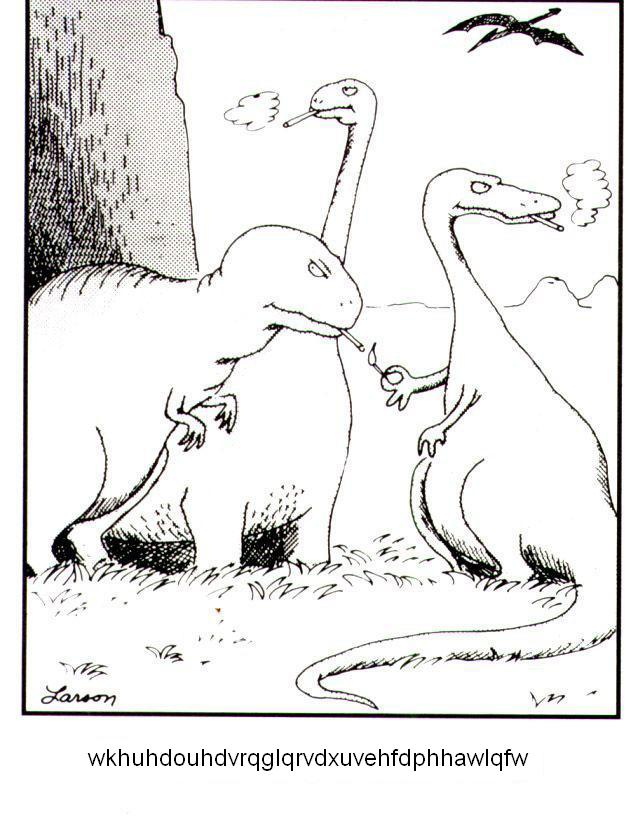
\includegraphics[width=5in]{dino-ciphertext.jpg}
\end{center}

\begin{center}
*** WARNING: SPOILERS ON THE NEXT PAGE *** 
\end{center}

\newpage
\begin{center}
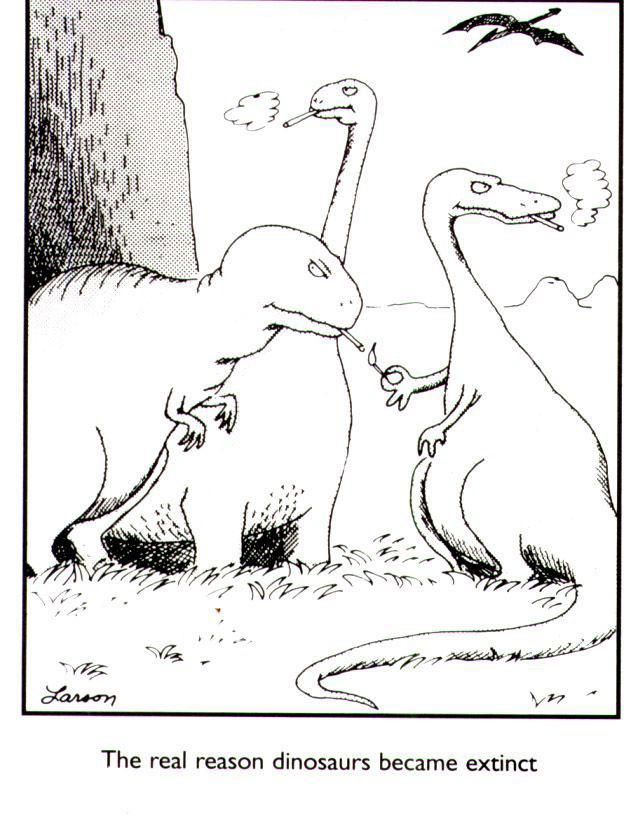
\includegraphics[width=5in]{dino-plaintext.jpg}
\end{center}


\begin{ex} 
  \label{ex:semigroup-associativity-0}
  \tinysidebar{\debug{exercises/{exercise-12/question.tex}}}
\mbox{}
  \begin{myenum}
  \item
    Solve
    \[
      5x^2 + y^2 = 3
    \]
    % mod 5, squares = 0^2=0, 1^2=1, 2^2=4, 3^2=4, 4^2=1
    (HINT: You don't really need number theory for this one. Why?
    But if you want to, imitate the solution for the previous
    problem.)
  \item
    Solve
    \[
      11y^2 - 5x^2 = 3
    \]
    % mod 5, squares = 0,1,4
    (HINT: This is just a slight change from the
    previous problem. \textit{But} now you need number theory. Try mod 4.
    If it does not work, try mod 5. Repeat.)
    % 3x^2 + y^2 = 3
    % {0,3} + {0,1} = 3
    % 0, 1, 3, 0 = 3
    % So x = 1, y = 0 (4)
    %
    % y^2=3 (5)
  \item
    Solve
    \[
      y^2 - 5x^2 = 2
    \]
    % mod 5, squares = 0^2=0, 1^2=1, 2^2=4, 3^2=4, 4^2=1    

  \item
    What about this one:
    \[
      x^2 - 5y^2 = 1
    \]    
  \end{myenum}
  {\scriptsize
[\textsc{Aside.}
Integer solutions to $x^2 - dy^2 = 1$ has been studied since at least 400BC.
This equation appear the Cattle Problem of Archimedes:

\begin{itemize}
  \item[]
If thou art diligent and wise, O stranger, compute the number of
cattle of the Sun, who once upon a time grazed on the fields of the
Thrinacian isle of Sicily, divided into four herds of different colours,
one milk white, another a glossy black, the third yellow and the last
dappled. In each herd were bulls, mighty in number according to these
proportions: Understand, stranger, that the white bulls were equal to
a half and a third of the black together with the whole of the yellow,
while the black were equal to the fourth part of the dappled and
a fifth, together with, once more, the whole of the yellow. Observe
further that the remaining bulls, the dappled, were equal to a sixth
part of the white and a seventh, together with all the yellow. These
were the proportions of the cows: The white were precisely equal to the
third part and a fourth of the whole herd of the black; while the black
were equal to the fourth part once more of the dappled and with it a
fifth part, when all, including the bulls went to pasture together. Now
the dappled in four parts8 were equal in number to a fifth part and a
sixth of the yellow herd. Finally the yellow were in number equal to
a sixth part and a seventh of the white herd. If thou canst accurately
tell, O stranger, the number of cattle of the Sun, giving separately the
number of well-fed bulls and again the number of females according
to each colour, thou wouldst not be called unskilled or ignorant of
numbers, but not yet shall thou be numbered among the wise. But
come, understand also all these conditions regarding the cows of the
Sun. When the white bulls mingled their number with the black, they
stood firm, equal in depth and breadth, and the plains of Thrinacia,
stretching far in all ways, were filled with their multitude. Again,
when the yellow and the dappled bulls were gathered into one herd
they stood in such a manner that their number, beginning from one,
grew slowly greater till it completed a triangular figure, there being
no bulls of other colours in their midst nor none of them lacking.
If thou art able, O stranger, to find out all these things and gather
them together in your mind, giving all the relations, thou shalt depart
crowned with glory and knowing that thou hast been adjudged perfect
in this species of wisdom.
\end{itemize}

If $W,X,Y,Z$ represents the number of white, black, yellow,
dappled bulls, you will get 
a systems of 7 linear equations, the first two being 
\begin{align*}
  W &= (1/2 + 1/3)X + Z \\
  X &= (1/4 + 1/5)Y + Z
\end{align*}
together with some constraints such as $W + X$ must be a square.
After some manipulations, it can be shown that the equation to solve looks like
\[
  x^2 - 410286423278424 y^2 = 1
\]
What was Archimedes thinking? You are find information on the Archimedes Cattle Problem on the web.]
}


  \solutionlink{sol:semigroup-associativity-0}
  \qed
\end{ex} 
\begin{python0}
from solutions import *
add(label="ex:semigroup-associativity-0",
    srcfilename='exercises/semigroup-associativity-0/answer.tex') 
\end{python0}


Let $P$ and $C$ be two sets.
A
\defone{cipher}
is just a pair of functions
$E: P \rightarrow C$ and $D: C \rightarrow P$
where $E$ is called the
\defone{encryption}
and $D$ is called the
\defone{decryption}
such that
\[
D(E(x)) = x \,\,\, \text{ for all } x \in P
\]
In other words
if you decrypt what you have encrypted, you get back the same data.
(It'd better be so!)
An element of $P$ is called a
\defone{plaintext} --
it's what you encrypt.
An element of $C$ is called a
\defone{ciphertext}
--
it's what you get when you encrypt.

Caesar cipher is an example of a cipher.
For Caesar cipher $P = C = \{a, b, c, ..., z\}$.
Also, although the encryption function maps one character to another,
it's understood that if you want to encrypt a string, you
simply encrypt each character of the string and join them up into
a string.

But if you allow the shift amount in the Caesar cipher to change,
then the encryption and decryption depends on the shift amount -- the key.
A general principle in cryptography is the following
concept due to
\href{https://en.wikipedia.org/wiki/Auguste_Kerckhoffs}{Auguste Kerckhoffs}:

\defone{Kerckhoffs' principle} (1883):
A secure cipher should not depend on the secrecy of the encryption
and decryption algorithm, but rather on the secrecy of the key.


The opposite and a really bad idea is called 
\defone{security through obscurity},
i.e., it's the hope that your
encrypted messages are safe as long as the encryption and decryption
algorithm are kept secret.

Why is this important?
Because it's easy to change the key while changing the encryption
and decryption algorithm might not be that easy.
If a worker who performs the encryption or decryption process is captured,
then he/she can be made (tortured?) to reveal the algorithm.
On the other hand, if the key is stolen, then we can simply change the key.
So in cryptography, it is always assumed that the algorithms (the cipher)
cannot be kept secret for long.

In fact in modern cryptography, once a cipher is designed,
the cryptography researcher(s) is expected to publish the cipher
so that other researchers can check if the cipher is actually secure.

So we just need to modify the definition of our cipher:

\begin{defn}
A
\defone{cipher}
is
a pair of functions
$E: K \times P \rightarrow C$ and
$D: K \times C \rightarrow P$ such that
if $k \in K$,
\[
D(k, E(k, x)) = x \,\,\, \text{ for all } x \in P
\]
$P$ is the set of plaintexts, $C$ is the set of ciphertexts,
and $K$ is the set of keys.
Notice that in the above the key used for encryption $k$
is the same as the key used for decryption.
\end{defn}

Instead of writing $E(k, x)$ and $D(k, x)$,
it's also common to write $E_{k}(x)$ and $D_{k}(x)$.
Depending on which book you read, the encryption and decryption functions
can also be written $e$ instead of $E$ and $d$ instead of $D$.

Humans have used ciphers for thousands of years.
The early ciphers always use the same key for encryption and decryption.
It was only very recently in 1970 that
\href{https://en.wikipedia.org/wiki/James_H._Ellis}{James H.~Ellis},
asked if it's possible to have a cipher that uses two distinct keys,
one for encryption and one for decryption.
Ellis was a British cryptographer at the
\href{https://en.wikipedia.org/wiki/GCHQ}{GCHQ }
(UK Government Communications
Headquarters).
If this is possible, then only the decyption key has to be kept secret.
Why do you want to a use such a cipher?

Well, I can publish the encryption key for such a cipher on a
website, you encrypt with the encryption key and send me the ciphertext by
email.
On receiving the ciphertext, I decrypt it using the decryption key.
Note that I can make the encryption key public, but I must keep
the decryption key a secret.
On the other hand for a symmetric key cipher, we would have to meet secretly
and decide on the common key.

Surprisingly such a cipher exists.

So now I have to modify our definition of ciphers ...

\begin{defn}
A
\defone{symmetric cipher}
is
a pair of functions
$E: K \times P \rightarrow C$ and
$D: K \times C \rightarrow P$ such that
if $k \in K$,
\[
D_k(E_k(x)) = x \,\,\, \text{ for all } x \in P
\]
$P$ is the set of plaintexts, $C$ is the set of ciphertexts,
and $K$ is the set of keys.
A symmetric cipher is also called a \defone{private key cipher}
because the key used must be kept private.
\end{defn}

And of course we also must have 

\begin{defn}
An
\defone{asymmetric cipher}
is a cipher where there are two distinct keys,
one for encryption and one for decryption.
An asymmetric cipher is also called a
\defone{public key cipher}
because the encryption key can be
made public (but the decryption key has to kept secret).
In this case, if $k,k'$ are the encryption and decryption keys,
then the cipher must satisfy
\[
D_{k'}(E_k(x)) = x
\]
for $x \in P$.
The encryption key $k$ is called the \defone{public key} (because it can be
made public)
while the decryption key is called the \defone{private key}.
\end{defn}


\begin{ex} 
  \label{ex:semigroup-associativity-0}
  \tinysidebar{\debug{exercises/{exercise-12/question.tex}}}
\mbox{}
  \begin{myenum}
  \item
    Solve
    \[
      5x^2 + y^2 = 3
    \]
    % mod 5, squares = 0^2=0, 1^2=1, 2^2=4, 3^2=4, 4^2=1
    (HINT: You don't really need number theory for this one. Why?
    But if you want to, imitate the solution for the previous
    problem.)
  \item
    Solve
    \[
      11y^2 - 5x^2 = 3
    \]
    % mod 5, squares = 0,1,4
    (HINT: This is just a slight change from the
    previous problem. \textit{But} now you need number theory. Try mod 4.
    If it does not work, try mod 5. Repeat.)
    % 3x^2 + y^2 = 3
    % {0,3} + {0,1} = 3
    % 0, 1, 3, 0 = 3
    % So x = 1, y = 0 (4)
    %
    % y^2=3 (5)
  \item
    Solve
    \[
      y^2 - 5x^2 = 2
    \]
    % mod 5, squares = 0^2=0, 1^2=1, 2^2=4, 3^2=4, 4^2=1    

  \item
    What about this one:
    \[
      x^2 - 5y^2 = 1
    \]    
  \end{myenum}
  {\scriptsize
[\textsc{Aside.}
Integer solutions to $x^2 - dy^2 = 1$ has been studied since at least 400BC.
This equation appear the Cattle Problem of Archimedes:

\begin{itemize}
  \item[]
If thou art diligent and wise, O stranger, compute the number of
cattle of the Sun, who once upon a time grazed on the fields of the
Thrinacian isle of Sicily, divided into four herds of different colours,
one milk white, another a glossy black, the third yellow and the last
dappled. In each herd were bulls, mighty in number according to these
proportions: Understand, stranger, that the white bulls were equal to
a half and a third of the black together with the whole of the yellow,
while the black were equal to the fourth part of the dappled and
a fifth, together with, once more, the whole of the yellow. Observe
further that the remaining bulls, the dappled, were equal to a sixth
part of the white and a seventh, together with all the yellow. These
were the proportions of the cows: The white were precisely equal to the
third part and a fourth of the whole herd of the black; while the black
were equal to the fourth part once more of the dappled and with it a
fifth part, when all, including the bulls went to pasture together. Now
the dappled in four parts8 were equal in number to a fifth part and a
sixth of the yellow herd. Finally the yellow were in number equal to
a sixth part and a seventh of the white herd. If thou canst accurately
tell, O stranger, the number of cattle of the Sun, giving separately the
number of well-fed bulls and again the number of females according
to each colour, thou wouldst not be called unskilled or ignorant of
numbers, but not yet shall thou be numbered among the wise. But
come, understand also all these conditions regarding the cows of the
Sun. When the white bulls mingled their number with the black, they
stood firm, equal in depth and breadth, and the plains of Thrinacia,
stretching far in all ways, were filled with their multitude. Again,
when the yellow and the dappled bulls were gathered into one herd
they stood in such a manner that their number, beginning from one,
grew slowly greater till it completed a triangular figure, there being
no bulls of other colours in their midst nor none of them lacking.
If thou art able, O stranger, to find out all these things and gather
them together in your mind, giving all the relations, thou shalt depart
crowned with glory and knowing that thou hast been adjudged perfect
in this species of wisdom.
\end{itemize}

If $W,X,Y,Z$ represents the number of white, black, yellow,
dappled bulls, you will get 
a systems of 7 linear equations, the first two being 
\begin{align*}
  W &= (1/2 + 1/3)X + Z \\
  X &= (1/4 + 1/5)Y + Z
\end{align*}
together with some constraints such as $W + X$ must be a square.
After some manipulations, it can be shown that the equation to solve looks like
\[
  x^2 - 410286423278424 y^2 = 1
\]
What was Archimedes thinking? You are find information on the Archimedes Cattle Problem on the web.]
}


  \solutionlink{sol:semigroup-associativity-0}
  \qed
\end{ex} 
\begin{python0}
from solutions import *
add(label="ex:semigroup-associativity-0",
    srcfilename='exercises/semigroup-associativity-0/answer.tex') 
\end{python0}


Public key ciphers use quite a bit of math.
So we won't see public key ciphers for a while.

Let's go back to our Caesar cipher.
You can think of the Caesar cipher as a special case of a symmetric cipher that
uses the key 3:
\begin{myenum}
\li encryption is \lq\lq shift forward by 3''
\li decryption is \lq\lq shift backward by 3''.
\end{myenum}
In other words, generalizing the Caesar cipher, we get the shift cipher:
\begin{myenum}
\li encryption is \lq\lq shift forward by $k$''
\li decryption is \lq\lq shift backward by $k$''.
\end{myenum}
where $k$ is the key.
I hope it's clear that the shift cipher with key 27 is
the same as the shift cipher with key 1.
Effectively speaking there are only 26 shifts, including
the very bad key of 0.
Hence for the shift cipher, $K = \{0, 1, 2, ..., 25\}$.

For classical ciphers, assuming we're only interested in English,
the plaintexts are
strings involving $a$-$z$.
I will write $\{a,b,c,...,z\}^*$ for the set of all strings with
characters from $\{a,b,c,...,z\}$.
If $n$ is a positive integer, I will also write $\{a,b,c,...,z\}^n$
for the set of strings with length $n$ and with characters
from the set $\{a,b,c,...,z\}$.
For instance
\[
\{a,b,c,...,z\}^2 = \{aa, ab, ac, ..., zx, zy, zz\}
\]


\begin{ex} 
  \label{ex:semigroup-associativity-0}
  \tinysidebar{\debug{exercises/{exercise-12/question.tex}}}
\mbox{}
  \begin{myenum}
  \item
    Solve
    \[
      5x^2 + y^2 = 3
    \]
    % mod 5, squares = 0^2=0, 1^2=1, 2^2=4, 3^2=4, 4^2=1
    (HINT: You don't really need number theory for this one. Why?
    But if you want to, imitate the solution for the previous
    problem.)
  \item
    Solve
    \[
      11y^2 - 5x^2 = 3
    \]
    % mod 5, squares = 0,1,4
    (HINT: This is just a slight change from the
    previous problem. \textit{But} now you need number theory. Try mod 4.
    If it does not work, try mod 5. Repeat.)
    % 3x^2 + y^2 = 3
    % {0,3} + {0,1} = 3
    % 0, 1, 3, 0 = 3
    % So x = 1, y = 0 (4)
    %
    % y^2=3 (5)
  \item
    Solve
    \[
      y^2 - 5x^2 = 2
    \]
    % mod 5, squares = 0^2=0, 1^2=1, 2^2=4, 3^2=4, 4^2=1    

  \item
    What about this one:
    \[
      x^2 - 5y^2 = 1
    \]    
  \end{myenum}
  {\scriptsize
[\textsc{Aside.}
Integer solutions to $x^2 - dy^2 = 1$ has been studied since at least 400BC.
This equation appear the Cattle Problem of Archimedes:

\begin{itemize}
  \item[]
If thou art diligent and wise, O stranger, compute the number of
cattle of the Sun, who once upon a time grazed on the fields of the
Thrinacian isle of Sicily, divided into four herds of different colours,
one milk white, another a glossy black, the third yellow and the last
dappled. In each herd were bulls, mighty in number according to these
proportions: Understand, stranger, that the white bulls were equal to
a half and a third of the black together with the whole of the yellow,
while the black were equal to the fourth part of the dappled and
a fifth, together with, once more, the whole of the yellow. Observe
further that the remaining bulls, the dappled, were equal to a sixth
part of the white and a seventh, together with all the yellow. These
were the proportions of the cows: The white were precisely equal to the
third part and a fourth of the whole herd of the black; while the black
were equal to the fourth part once more of the dappled and with it a
fifth part, when all, including the bulls went to pasture together. Now
the dappled in four parts8 were equal in number to a fifth part and a
sixth of the yellow herd. Finally the yellow were in number equal to
a sixth part and a seventh of the white herd. If thou canst accurately
tell, O stranger, the number of cattle of the Sun, giving separately the
number of well-fed bulls and again the number of females according
to each colour, thou wouldst not be called unskilled or ignorant of
numbers, but not yet shall thou be numbered among the wise. But
come, understand also all these conditions regarding the cows of the
Sun. When the white bulls mingled their number with the black, they
stood firm, equal in depth and breadth, and the plains of Thrinacia,
stretching far in all ways, were filled with their multitude. Again,
when the yellow and the dappled bulls were gathered into one herd
they stood in such a manner that their number, beginning from one,
grew slowly greater till it completed a triangular figure, there being
no bulls of other colours in their midst nor none of them lacking.
If thou art able, O stranger, to find out all these things and gather
them together in your mind, giving all the relations, thou shalt depart
crowned with glory and knowing that thou hast been adjudged perfect
in this species of wisdom.
\end{itemize}

If $W,X,Y,Z$ represents the number of white, black, yellow,
dappled bulls, you will get 
a systems of 7 linear equations, the first two being 
\begin{align*}
  W &= (1/2 + 1/3)X + Z \\
  X &= (1/4 + 1/5)Y + Z
\end{align*}
together with some constraints such as $W + X$ must be a square.
After some manipulations, it can be shown that the equation to solve looks like
\[
  x^2 - 410286423278424 y^2 = 1
\]
What was Archimedes thinking? You are find information on the Archimedes Cattle Problem on the web.]
}


  \solutionlink{sol:semigroup-associativity-0}
  \qed
\end{ex} 
\begin{python0}
from solutions import *
add(label="ex:semigroup-associativity-0",
    srcfilename='exercises/semigroup-associativity-0/answer.tex') 
\end{python0}


In modern day cryptography, we frequently work with bit strings.
The set of all bit strings is denoted by $\{0,1\}^*$.
Bit strings of length exactly 8 is denoted by $\{0,1\}^8$ --
these would be bytes.
For instance you might have heard of the SHA2 family of hash function.
SHA256 takes in bit strings and spits out bit strings of length 256.
So SHA256 is a function of type
\[
\{0,1\}^* \rightarrow \{0,1\}^8
\]
(Technically speaking SHA256 inputs do have a maximum limit in length,
but it's so huge that for practical purposes it's as good as all possible bit
strings.)

You know this is coming ... we'll be using
\textit{lots} of math to do 
encryption and decryption.
In particular, for this notes, we associate letters $a$ to $z$ with numbers.
The encryption and decryption function will work with either numbers of 
letters.
Specifically we have the following correspondence:
\sidebar{
In math, \lq\lq correspondence'' is the same as 
\lq\lq 1-1 correspondence'' which is the same as
\lq\lq bijection''.
Remember bijection?
It's time to check your discrete math notes}
\begin{align*}
a &\leftrightarrow 0 \\
b &\leftrightarrow 1 \\
c &\leftrightarrow 2 \\
\vdots  &\textwhite{\leftarrow 2} \vdots \\
z &\leftrightarrow 25
\end{align*}

if $E$ encrypts $a$ to $c$, I will say either 
\[
E(a) = c
\]
or 
\[
E(0) = 2
\]

Now you might say ... \lq\lq so what's the big deal? 
Why rewrite $a$ as $0$,  $b$ as $1$, etc.
I can also come up with some secret encoding for instance
why can't I rewrite $a$ as a square, $b$ as a triangle, etc.?''

Well ... the reason is because $0, 1, 2, ...$ are numbers ... and ...
\textit{they have operations (addition, subtraction, multiplication, division).}

With the above in mind, instead of describing the shift cipher as
functions on $a$-$z$, I'll describe it as function on $\Z/26$:

\begin{defn}
The \defone{shift cipher} $(E, D)$ is given by
\[
  E_k(x) = x + k \pmod{26}
\]
and
\[
  D_k(x) = x - k \pmod{26}
\]
\end{defn}

It's clear that for the shift cipher $(E, D)$,
\[
D_k(E_k(x)) \equiv x \pmod{26}
\]

And of course the shift cipher with key $k = 3$ is the \defone{Caesar cipher}.

\newpage\sectionthree{Modular arithmetic}
\begin{python0}
from solutions import *; clear()
\end{python0}

Number theory is basically the study of whole numbers.
That however is an over-simplification.
The study of number theory involves almost all areas of mathematics.
In fact many areas of mathematics were created just to study 
certain problems in number theory.

Number theory is an extremely huge area of study in Mathematics and Computer
Science. It is also extremely fascinating. Many problems is number theory can
be stated very simply so that even a high school student can understand the
statement of the problem. And yet the techniques used to solve some of these
problems require the mathematical tools from almost every area of Math. Gauss
once said that ``Mathematics is the queen of sciences and number theory is the
queen of mathematics".

Although there are many branches within Number Theory, right now
we only need to know a little bit about Elementary Number Theory.
``Elementary" here does not mean simple (although it will be for
us since you're only seeing a small part of Elementary Number
Theory). It means we are studying Number Theory using only
properties of whole numbers (integers). Research in Number Theory
requires real numbers, complex numbers, calculus, geometry,
complex analysis, etc.

This will be a very short introduction to the vast area of Number
Theory. In fact this is only a tiny fraction of Elementary Number
Theory. This is one of the oldest area of Mathematics and one of
the fascinating because of its history. If you want to learn more
about number theory, just let me know. I can easily find a project
for you to work on.

For now, we will look at modular arithmetic.
Besides cryptography,
modular arithmetic is also used in
data compression and error correction codes.

The set of integers $\{..., -3, -2, -1, 0, 1, 2, 3, ...\}$
denoted $\Z$ has two operations $+$ and $\cdot$.
In terms of the algebraic structure (i.e. the operations), $\Z$ is known as
a \textbf{commutative ring}.
Basically a commutative ring is a set of \lq\lq things'' with
two operations, addition and multiplication, with rules that
look like the addition and multiplication rules for $\Z$.
For instance one such rule in $\Z$ is
\[
  a (b + c) = ab + ac
\]
This same rule holds true for $\Q$, $\R$, $\C$ and polynomials with coefficients in $\Z$.

The reason why mathematicians even bother defining this concept
of \lq\lq commutative ring"
is more or less
the same reason why we write functions in programs: for re-use.
There are \textit{many} naturally occurring rings.
So if while developing the theory for 
$\token{\operatorname{blah_1}}$
and
$\token{\operatorname{blah_2}}$
and they are both rings, then it's enough to prove a general fact that applies
to both and quote the fact.
This is also related to the concept of inheritance and abstract base classes.
You can think of $\Z, \Q, \R, \C$ as subclasses of \verb!CommutativeRing!.
Therefore if you have a function
\begin{console}
void f(CommutativeRing & r)
{
  ...
}
\end{console}
then \verb!f! can work with \verb!x! if \verb!x! is a object of $\Z, \Q, \R, \C$.

The mathematician develop  general results while the programmer
write general functions working on abstract base class objects.
The idea is the same.
The reason for generality is efficiency.

Here's a very important advice on studying rings, groups, fields, math, etc.
(in fact this applies to any area of study where there is a great deal of 
generalization):
Although the definition and theorems are general, you
\textit{always} keep a
couple of standard examples in your mind as you read the statements.
While reading them, mentally substitute your examples into the facts so that 
you can associate it to something more concrete.
This is not just a learn technique for undergraduate students.
Even researchers do that when they read research papers.
For the definition of ring below, think of the ring of integers.

I will try to be as informal as possible for now
so that you can develop some feel/intuition for what we need for now.
Later I'm going to come back to this topic and redo the whole thing rigorously.
The focus for now is to understand modulo 26 arithmetic.

Anyway, a \textbf{commutatative ring} $R$ 
\sidenote{
Example: the integer $\Z$,...$+$ and $\cdot$ of $\Z$ ...
}
is a set of \lq\lq things''
with two operations abstractly denoted by 
$\oplus$ and $\odot$ (\lq\lq addition'' and \lq\lq multiplication'')
Furthermore there are two special \lq\lq things'' in $R$ which we will call
$0_R$ and $1_R$.
The properties satisfied by $R,0_R,1_R,\oplus,\odot$ 
\sidebar{
0 and 1 of $\Z$ ...
}
(of course there must be
something satisfied by them!) are as follows.
For $\oplus$ the properties are:
\begin{myenum}
\item $r \oplus s$ is in $R$ for all $r,s$ in $R$
\sidebar{$i + j$ is in $\Z$ for integers $i$, $j$, ...}
\item 
$(r \oplus s) \oplus t
=
r \oplus (s \oplus t)$
for all $r,s,t$ in $R$
\sidebar{
$(i + j) + k = i + (j + k)$
for integers $i,j,k$ ...
}
\item
$r \oplus 0_R = r = 0_R \oplus r$ 
for all
$r$ in $R$
\sidebar{
$i + 0 = i = 0 + i$
for integer $i$ ...
}
\item For 
\sidebar{
If $i$ is an integer, then $-i$ is also an integer and 
$i + (-i)= 0 =$
$(-i)+ i$.
}
all $r$ in $R$ there is something in $R$ which we will call $r'$
such that $r \oplus r' =$ $0_R = r' \oplus r$
\end{myenum}
For $\odot$ the properties are:
\begin{myenum}
\item $r \odot s$ is in $R$ for all $r, s$ in $R$
\sidebar{$ij = ji$ for integer $i,j$,...}
\item $(r \odot s) \odot t = r \odot (s \odot t)$ for all $r,s,t$ in $R$
\sidebar{
$(ij)k = i(jk)$ for integers $i,j,k$
}
\item $r \odot 1_R = r = 1_R \odot r$ for all $r$ in $R$
\sidebar{
$i1 = i = 1i$ for integer $i$ ...
}
\item $r \odot s = s \odot r$ for all $r,s$ in $R$ 
\sidebar{
$ij = ji$ for integers $i,j$
}
\end{myenum}
The property involving both $\oplus$ and $\odot$ is
\begin{myenum}
\item 
$r \odot (s \oplus t) =$
$r \odot s \oplus r\odot t$
\sidebar{
$i(j + k) = ij + ik$ for integers $i,j,k$.
Phew! So $\Z$ is a commutative ring.
}
\end{myenum}

Just remember this: 
A ring is a set of things with addition and multiplication.
And when you're lost just think of the set of integers and its operations.

Now we'll be working with the alphabet a,b,...,z.
We'll call them by their new identities: $0,1,...,25$.
This is not exactly all of $\Z$.
The formulas for the encryption and decryption of Caesar's cipher
involves addition and
substraction.
What if we go beyond? 
What is 3 + 25 (i.e., d + z)?
No problem, we will take remainders mod 26.
\sidebar{In C\texttt{++}-speak, we take $\% 26$.}
So instead of 3 + 25 we think of (3 + 25) mod 26 instead.
Of course the remainders are 0, 1, ..., 25 which is exactly what we want. 

To indicate that we're only interested in remainders or more accurately, we ignore multiples of 26, we write
\begin{align*}
3 + 25 
&= 28 \\
&\equiv 2 \pmod{26}
\end{align*}
In general, if $x$ and $y$ are integers, we write
\[
x \equiv y \pmod{26}
\]
if 26 divides $x - y$.
It does not mean that $x$ is equal to $y$.
It means that $x$ and $y$ are the same if you ignore additive multiples of 26, i.e.,
\[
x \equiv y \pmod{26}
\]
is the same as saying
\[
  x = y + (\text{... some multiple of 26 ...})
\]
This is the same as saying the remainder when $x$ is divided by 26
is the same as the remainder when $y$ is divided by 26.

If two numbers differ by a multiple of 26, we say that they are
\defone{congruent} mod 26.

Note that
\begin{align*}
26 &\equiv 0 \pmod{26} \\   
27 &\equiv 1 \pmod{26} \\
  28 &\equiv 2 \pmod{26} \\
  ...
\end{align*}
and
\begin{align*}
-1 &\equiv 25 \pmod{26} \\   
-2 &\equiv 24 \pmod{26} \\
-3 &\equiv 23 \pmod{26} \\
  ...
\end{align*}
So in the mod 26 world, since you are ignoring multiples of 26,
\textit{in some sense} there are only 26 numbers:
\[
  0, 1, 2, 3, ..., 25
\]
I'll write $\Z/26$ for this world of 26 values.
Remember that in this world, you can write the symbol
\[
  28
\]
but this is the same as 2 in $\Z/26$:
\[
  28 \equiv 2 \pmod{26}
\]
Of course in $\Z$, these symbols, i.e. $28$ and $2$, are different.

Most of the algebraic rules involving $+, -, *, 0, 1$ applies when
working with integers mod 26.
For instance suppose 
\[
  x \equiv y \pmod{26}
\]
where $x$ and $y$ are integers
(i.e., $x$ differs from $y$ by a multiple of 26), then
\[
  x + z \equiv y + z\pmod{26}
\]
where $z$ is an integer.
Likewise
from
\[
  x \equiv y \pmod{26}
\]
we get
\[
  x z \equiv y z \pmod{26}
\]
It's also true that
\[
  0 + x \equiv x \pmod{26}
\]
and 
\[
  1 \cdot x \equiv x \pmod{26}
\]

To be more precise, $\Z/26$ is a commutative ring.
It's a finite commutative ring with 26 values.
Let me rewrite the axioms for a commutative ring for $\Z/26$.

For $+$ on $\Z/26$, the properties are:
\begin{myenum}
\item $(r + s) \pmod{26}$ is in $\Z/26$ for all $r,s$ in $\Z/26$
\item 
  $(r + s) + t
  \equiv
  r + (s + t) \pmod{26}$
for all $r,s,t$ in $\Z/26$
\item
$r + 0 \equiv r \equiv 0 + r \pmod{26}$ 
for all
$r$ in $\Z/26$.
In fact $r'$ is just $(26 - r) \pmod{26}$.
For instance for $r = 2 \pmod{26}$, $r' = 26 - 2 = 24 \pmod{26}$.
\item For 
all $r$ in $\Z/26$ there is something in $\Z/26$ which we will call $r'$
such that $r + r' \equiv 0 \equiv r' \oplus r \pmod{26}$
\end{myenum}

For $\cdot$ the properties are:
\begin{myenum}
\item $r \cdot s \pmod{26}$ is in $\Z/26$ for all $r, s$ in $\Z/26$
\item $(r \cdot s) \cdot t \equiv r \cdot (s \cdot t) \pmod{26}$ for all $r,s,t$ in $\Z/26$
\item $r \cdot 1 \equiv r \equiv 1 \cdot r \pmod{26}$ for all $r$ in $\Z/26$
\item $r \cdot s \equiv s \cdot r \pmod{26}$ for all $r,s$ in $\Z/26$ 
\end{myenum}
The property involving both $+$ and $\cdot$ is
\begin{myenum}
\item 
$r \cdot (s + t) \equiv$
$r \cdot s + r \cdot t \pmod{26}$
\end{myenum}

It's also not too surprising that you can talk about mod $n$ for any
positive integer $n$.

If I don't say so, when I want you write some $x \pmod{26}$, I mean the $x$
such that $0 \leq x < 26$.
Of course there's no difference in mod 26 between 2 and 28.
But in mod 26, the values in $[0, 26)$ is the preferred range.
Also, when I say simplify $27 \pmod{26}$, I mean $1 \pmod{26}$.

Note that since $\Z/26$ is \textit{finite}, you can always solve
any equation in mod 26.
This is similar to boolean values: there are only two.
To solve a boolean equation, you just try all possible boolean values.
So to solve a $\Z/26$ equation, you just try all the 26 possible
values on all the variables that appear in the equation.


\begin{ex} 
  \label{ex:semigroup-associativity-0}
  \tinysidebar{\debug{exercises/{exercise-12/question.tex}}}
\mbox{}
  \begin{myenum}
  \item
    Solve
    \[
      5x^2 + y^2 = 3
    \]
    % mod 5, squares = 0^2=0, 1^2=1, 2^2=4, 3^2=4, 4^2=1
    (HINT: You don't really need number theory for this one. Why?
    But if you want to, imitate the solution for the previous
    problem.)
  \item
    Solve
    \[
      11y^2 - 5x^2 = 3
    \]
    % mod 5, squares = 0,1,4
    (HINT: This is just a slight change from the
    previous problem. \textit{But} now you need number theory. Try mod 4.
    If it does not work, try mod 5. Repeat.)
    % 3x^2 + y^2 = 3
    % {0,3} + {0,1} = 3
    % 0, 1, 3, 0 = 3
    % So x = 1, y = 0 (4)
    %
    % y^2=3 (5)
  \item
    Solve
    \[
      y^2 - 5x^2 = 2
    \]
    % mod 5, squares = 0^2=0, 1^2=1, 2^2=4, 3^2=4, 4^2=1    

  \item
    What about this one:
    \[
      x^2 - 5y^2 = 1
    \]    
  \end{myenum}
  {\scriptsize
[\textsc{Aside.}
Integer solutions to $x^2 - dy^2 = 1$ has been studied since at least 400BC.
This equation appear the Cattle Problem of Archimedes:

\begin{itemize}
  \item[]
If thou art diligent and wise, O stranger, compute the number of
cattle of the Sun, who once upon a time grazed on the fields of the
Thrinacian isle of Sicily, divided into four herds of different colours,
one milk white, another a glossy black, the third yellow and the last
dappled. In each herd were bulls, mighty in number according to these
proportions: Understand, stranger, that the white bulls were equal to
a half and a third of the black together with the whole of the yellow,
while the black were equal to the fourth part of the dappled and
a fifth, together with, once more, the whole of the yellow. Observe
further that the remaining bulls, the dappled, were equal to a sixth
part of the white and a seventh, together with all the yellow. These
were the proportions of the cows: The white were precisely equal to the
third part and a fourth of the whole herd of the black; while the black
were equal to the fourth part once more of the dappled and with it a
fifth part, when all, including the bulls went to pasture together. Now
the dappled in four parts8 were equal in number to a fifth part and a
sixth of the yellow herd. Finally the yellow were in number equal to
a sixth part and a seventh of the white herd. If thou canst accurately
tell, O stranger, the number of cattle of the Sun, giving separately the
number of well-fed bulls and again the number of females according
to each colour, thou wouldst not be called unskilled or ignorant of
numbers, but not yet shall thou be numbered among the wise. But
come, understand also all these conditions regarding the cows of the
Sun. When the white bulls mingled their number with the black, they
stood firm, equal in depth and breadth, and the plains of Thrinacia,
stretching far in all ways, were filled with their multitude. Again,
when the yellow and the dappled bulls were gathered into one herd
they stood in such a manner that their number, beginning from one,
grew slowly greater till it completed a triangular figure, there being
no bulls of other colours in their midst nor none of them lacking.
If thou art able, O stranger, to find out all these things and gather
them together in your mind, giving all the relations, thou shalt depart
crowned with glory and knowing that thou hast been adjudged perfect
in this species of wisdom.
\end{itemize}

If $W,X,Y,Z$ represents the number of white, black, yellow,
dappled bulls, you will get 
a systems of 7 linear equations, the first two being 
\begin{align*}
  W &= (1/2 + 1/3)X + Z \\
  X &= (1/4 + 1/5)Y + Z
\end{align*}
together with some constraints such as $W + X$ must be a square.
After some manipulations, it can be shown that the equation to solve looks like
\[
  x^2 - 410286423278424 y^2 = 1
\]
What was Archimedes thinking? You are find information on the Archimedes Cattle Problem on the web.]
}


  \solutionlink{sol:semigroup-associativity-0}
  \qed
\end{ex} 
\begin{python0}
from solutions import *
add(label="ex:semigroup-associativity-0",
    srcfilename='exercises/semigroup-associativity-0/answer.tex') 
\end{python0}


\begin{ex} 
  \label{ex:semigroup-associativity-0}
  \tinysidebar{\debug{exercises/{exercise-12/question.tex}}}
\mbox{}
  \begin{myenum}
  \item
    Solve
    \[
      5x^2 + y^2 = 3
    \]
    % mod 5, squares = 0^2=0, 1^2=1, 2^2=4, 3^2=4, 4^2=1
    (HINT: You don't really need number theory for this one. Why?
    But if you want to, imitate the solution for the previous
    problem.)
  \item
    Solve
    \[
      11y^2 - 5x^2 = 3
    \]
    % mod 5, squares = 0,1,4
    (HINT: This is just a slight change from the
    previous problem. \textit{But} now you need number theory. Try mod 4.
    If it does not work, try mod 5. Repeat.)
    % 3x^2 + y^2 = 3
    % {0,3} + {0,1} = 3
    % 0, 1, 3, 0 = 3
    % So x = 1, y = 0 (4)
    %
    % y^2=3 (5)
  \item
    Solve
    \[
      y^2 - 5x^2 = 2
    \]
    % mod 5, squares = 0^2=0, 1^2=1, 2^2=4, 3^2=4, 4^2=1    

  \item
    What about this one:
    \[
      x^2 - 5y^2 = 1
    \]    
  \end{myenum}
  {\scriptsize
[\textsc{Aside.}
Integer solutions to $x^2 - dy^2 = 1$ has been studied since at least 400BC.
This equation appear the Cattle Problem of Archimedes:

\begin{itemize}
  \item[]
If thou art diligent and wise, O stranger, compute the number of
cattle of the Sun, who once upon a time grazed on the fields of the
Thrinacian isle of Sicily, divided into four herds of different colours,
one milk white, another a glossy black, the third yellow and the last
dappled. In each herd were bulls, mighty in number according to these
proportions: Understand, stranger, that the white bulls were equal to
a half and a third of the black together with the whole of the yellow,
while the black were equal to the fourth part of the dappled and
a fifth, together with, once more, the whole of the yellow. Observe
further that the remaining bulls, the dappled, were equal to a sixth
part of the white and a seventh, together with all the yellow. These
were the proportions of the cows: The white were precisely equal to the
third part and a fourth of the whole herd of the black; while the black
were equal to the fourth part once more of the dappled and with it a
fifth part, when all, including the bulls went to pasture together. Now
the dappled in four parts8 were equal in number to a fifth part and a
sixth of the yellow herd. Finally the yellow were in number equal to
a sixth part and a seventh of the white herd. If thou canst accurately
tell, O stranger, the number of cattle of the Sun, giving separately the
number of well-fed bulls and again the number of females according
to each colour, thou wouldst not be called unskilled or ignorant of
numbers, but not yet shall thou be numbered among the wise. But
come, understand also all these conditions regarding the cows of the
Sun. When the white bulls mingled their number with the black, they
stood firm, equal in depth and breadth, and the plains of Thrinacia,
stretching far in all ways, were filled with their multitude. Again,
when the yellow and the dappled bulls were gathered into one herd
they stood in such a manner that their number, beginning from one,
grew slowly greater till it completed a triangular figure, there being
no bulls of other colours in their midst nor none of them lacking.
If thou art able, O stranger, to find out all these things and gather
them together in your mind, giving all the relations, thou shalt depart
crowned with glory and knowing that thou hast been adjudged perfect
in this species of wisdom.
\end{itemize}

If $W,X,Y,Z$ represents the number of white, black, yellow,
dappled bulls, you will get 
a systems of 7 linear equations, the first two being 
\begin{align*}
  W &= (1/2 + 1/3)X + Z \\
  X &= (1/4 + 1/5)Y + Z
\end{align*}
together with some constraints such as $W + X$ must be a square.
After some manipulations, it can be shown that the equation to solve looks like
\[
  x^2 - 410286423278424 y^2 = 1
\]
What was Archimedes thinking? You are find information on the Archimedes Cattle Problem on the web.]
}


  \solutionlink{sol:semigroup-associativity-0}
  \qed
\end{ex} 
\begin{python0}
from solutions import *
add(label="ex:semigroup-associativity-0",
    srcfilename='exercises/semigroup-associativity-0/answer.tex') 
\end{python0}


\begin{ex} 
  \label{ex:semigroup-associativity-0}
  \tinysidebar{\debug{exercises/{exercise-12/question.tex}}}
\mbox{}
  \begin{myenum}
  \item
    Solve
    \[
      5x^2 + y^2 = 3
    \]
    % mod 5, squares = 0^2=0, 1^2=1, 2^2=4, 3^2=4, 4^2=1
    (HINT: You don't really need number theory for this one. Why?
    But if you want to, imitate the solution for the previous
    problem.)
  \item
    Solve
    \[
      11y^2 - 5x^2 = 3
    \]
    % mod 5, squares = 0,1,4
    (HINT: This is just a slight change from the
    previous problem. \textit{But} now you need number theory. Try mod 4.
    If it does not work, try mod 5. Repeat.)
    % 3x^2 + y^2 = 3
    % {0,3} + {0,1} = 3
    % 0, 1, 3, 0 = 3
    % So x = 1, y = 0 (4)
    %
    % y^2=3 (5)
  \item
    Solve
    \[
      y^2 - 5x^2 = 2
    \]
    % mod 5, squares = 0^2=0, 1^2=1, 2^2=4, 3^2=4, 4^2=1    

  \item
    What about this one:
    \[
      x^2 - 5y^2 = 1
    \]    
  \end{myenum}
  {\scriptsize
[\textsc{Aside.}
Integer solutions to $x^2 - dy^2 = 1$ has been studied since at least 400BC.
This equation appear the Cattle Problem of Archimedes:

\begin{itemize}
  \item[]
If thou art diligent and wise, O stranger, compute the number of
cattle of the Sun, who once upon a time grazed on the fields of the
Thrinacian isle of Sicily, divided into four herds of different colours,
one milk white, another a glossy black, the third yellow and the last
dappled. In each herd were bulls, mighty in number according to these
proportions: Understand, stranger, that the white bulls were equal to
a half and a third of the black together with the whole of the yellow,
while the black were equal to the fourth part of the dappled and
a fifth, together with, once more, the whole of the yellow. Observe
further that the remaining bulls, the dappled, were equal to a sixth
part of the white and a seventh, together with all the yellow. These
were the proportions of the cows: The white were precisely equal to the
third part and a fourth of the whole herd of the black; while the black
were equal to the fourth part once more of the dappled and with it a
fifth part, when all, including the bulls went to pasture together. Now
the dappled in four parts8 were equal in number to a fifth part and a
sixth of the yellow herd. Finally the yellow were in number equal to
a sixth part and a seventh of the white herd. If thou canst accurately
tell, O stranger, the number of cattle of the Sun, giving separately the
number of well-fed bulls and again the number of females according
to each colour, thou wouldst not be called unskilled or ignorant of
numbers, but not yet shall thou be numbered among the wise. But
come, understand also all these conditions regarding the cows of the
Sun. When the white bulls mingled their number with the black, they
stood firm, equal in depth and breadth, and the plains of Thrinacia,
stretching far in all ways, were filled with their multitude. Again,
when the yellow and the dappled bulls were gathered into one herd
they stood in such a manner that their number, beginning from one,
grew slowly greater till it completed a triangular figure, there being
no bulls of other colours in their midst nor none of them lacking.
If thou art able, O stranger, to find out all these things and gather
them together in your mind, giving all the relations, thou shalt depart
crowned with glory and knowing that thou hast been adjudged perfect
in this species of wisdom.
\end{itemize}

If $W,X,Y,Z$ represents the number of white, black, yellow,
dappled bulls, you will get 
a systems of 7 linear equations, the first two being 
\begin{align*}
  W &= (1/2 + 1/3)X + Z \\
  X &= (1/4 + 1/5)Y + Z
\end{align*}
together with some constraints such as $W + X$ must be a square.
After some manipulations, it can be shown that the equation to solve looks like
\[
  x^2 - 410286423278424 y^2 = 1
\]
What was Archimedes thinking? You are find information on the Archimedes Cattle Problem on the web.]
}


  \solutionlink{sol:semigroup-associativity-0}
  \qed
\end{ex} 
\begin{python0}
from solutions import *
add(label="ex:semigroup-associativity-0",
    srcfilename='exercises/semigroup-associativity-0/answer.tex') 
\end{python0}


\begin{ex} 
  \label{ex:semigroup-associativity-0}
  \tinysidebar{\debug{exercises/{exercise-12/question.tex}}}
\mbox{}
  \begin{myenum}
  \item
    Solve
    \[
      5x^2 + y^2 = 3
    \]
    % mod 5, squares = 0^2=0, 1^2=1, 2^2=4, 3^2=4, 4^2=1
    (HINT: You don't really need number theory for this one. Why?
    But if you want to, imitate the solution for the previous
    problem.)
  \item
    Solve
    \[
      11y^2 - 5x^2 = 3
    \]
    % mod 5, squares = 0,1,4
    (HINT: This is just a slight change from the
    previous problem. \textit{But} now you need number theory. Try mod 4.
    If it does not work, try mod 5. Repeat.)
    % 3x^2 + y^2 = 3
    % {0,3} + {0,1} = 3
    % 0, 1, 3, 0 = 3
    % So x = 1, y = 0 (4)
    %
    % y^2=3 (5)
  \item
    Solve
    \[
      y^2 - 5x^2 = 2
    \]
    % mod 5, squares = 0^2=0, 1^2=1, 2^2=4, 3^2=4, 4^2=1    

  \item
    What about this one:
    \[
      x^2 - 5y^2 = 1
    \]    
  \end{myenum}
  {\scriptsize
[\textsc{Aside.}
Integer solutions to $x^2 - dy^2 = 1$ has been studied since at least 400BC.
This equation appear the Cattle Problem of Archimedes:

\begin{itemize}
  \item[]
If thou art diligent and wise, O stranger, compute the number of
cattle of the Sun, who once upon a time grazed on the fields of the
Thrinacian isle of Sicily, divided into four herds of different colours,
one milk white, another a glossy black, the third yellow and the last
dappled. In each herd were bulls, mighty in number according to these
proportions: Understand, stranger, that the white bulls were equal to
a half and a third of the black together with the whole of the yellow,
while the black were equal to the fourth part of the dappled and
a fifth, together with, once more, the whole of the yellow. Observe
further that the remaining bulls, the dappled, were equal to a sixth
part of the white and a seventh, together with all the yellow. These
were the proportions of the cows: The white were precisely equal to the
third part and a fourth of the whole herd of the black; while the black
were equal to the fourth part once more of the dappled and with it a
fifth part, when all, including the bulls went to pasture together. Now
the dappled in four parts8 were equal in number to a fifth part and a
sixth of the yellow herd. Finally the yellow were in number equal to
a sixth part and a seventh of the white herd. If thou canst accurately
tell, O stranger, the number of cattle of the Sun, giving separately the
number of well-fed bulls and again the number of females according
to each colour, thou wouldst not be called unskilled or ignorant of
numbers, but not yet shall thou be numbered among the wise. But
come, understand also all these conditions regarding the cows of the
Sun. When the white bulls mingled their number with the black, they
stood firm, equal in depth and breadth, and the plains of Thrinacia,
stretching far in all ways, were filled with their multitude. Again,
when the yellow and the dappled bulls were gathered into one herd
they stood in such a manner that their number, beginning from one,
grew slowly greater till it completed a triangular figure, there being
no bulls of other colours in their midst nor none of them lacking.
If thou art able, O stranger, to find out all these things and gather
them together in your mind, giving all the relations, thou shalt depart
crowned with glory and knowing that thou hast been adjudged perfect
in this species of wisdom.
\end{itemize}

If $W,X,Y,Z$ represents the number of white, black, yellow,
dappled bulls, you will get 
a systems of 7 linear equations, the first two being 
\begin{align*}
  W &= (1/2 + 1/3)X + Z \\
  X &= (1/4 + 1/5)Y + Z
\end{align*}
together with some constraints such as $W + X$ must be a square.
After some manipulations, it can be shown that the equation to solve looks like
\[
  x^2 - 410286423278424 y^2 = 1
\]
What was Archimedes thinking? You are find information on the Archimedes Cattle Problem on the web.]
}


  \solutionlink{sol:semigroup-associativity-0}
  \qed
\end{ex} 
\begin{python0}
from solutions import *
add(label="ex:semigroup-associativity-0",
    srcfilename='exercises/semigroup-associativity-0/answer.tex') 
\end{python0}


\begin{ex} 
  \label{ex:semigroup-associativity-0}
  \tinysidebar{\debug{exercises/{exercise-12/question.tex}}}
\mbox{}
  \begin{myenum}
  \item
    Solve
    \[
      5x^2 + y^2 = 3
    \]
    % mod 5, squares = 0^2=0, 1^2=1, 2^2=4, 3^2=4, 4^2=1
    (HINT: You don't really need number theory for this one. Why?
    But if you want to, imitate the solution for the previous
    problem.)
  \item
    Solve
    \[
      11y^2 - 5x^2 = 3
    \]
    % mod 5, squares = 0,1,4
    (HINT: This is just a slight change from the
    previous problem. \textit{But} now you need number theory. Try mod 4.
    If it does not work, try mod 5. Repeat.)
    % 3x^2 + y^2 = 3
    % {0,3} + {0,1} = 3
    % 0, 1, 3, 0 = 3
    % So x = 1, y = 0 (4)
    %
    % y^2=3 (5)
  \item
    Solve
    \[
      y^2 - 5x^2 = 2
    \]
    % mod 5, squares = 0^2=0, 1^2=1, 2^2=4, 3^2=4, 4^2=1    

  \item
    What about this one:
    \[
      x^2 - 5y^2 = 1
    \]    
  \end{myenum}
  {\scriptsize
[\textsc{Aside.}
Integer solutions to $x^2 - dy^2 = 1$ has been studied since at least 400BC.
This equation appear the Cattle Problem of Archimedes:

\begin{itemize}
  \item[]
If thou art diligent and wise, O stranger, compute the number of
cattle of the Sun, who once upon a time grazed on the fields of the
Thrinacian isle of Sicily, divided into four herds of different colours,
one milk white, another a glossy black, the third yellow and the last
dappled. In each herd were bulls, mighty in number according to these
proportions: Understand, stranger, that the white bulls were equal to
a half and a third of the black together with the whole of the yellow,
while the black were equal to the fourth part of the dappled and
a fifth, together with, once more, the whole of the yellow. Observe
further that the remaining bulls, the dappled, were equal to a sixth
part of the white and a seventh, together with all the yellow. These
were the proportions of the cows: The white were precisely equal to the
third part and a fourth of the whole herd of the black; while the black
were equal to the fourth part once more of the dappled and with it a
fifth part, when all, including the bulls went to pasture together. Now
the dappled in four parts8 were equal in number to a fifth part and a
sixth of the yellow herd. Finally the yellow were in number equal to
a sixth part and a seventh of the white herd. If thou canst accurately
tell, O stranger, the number of cattle of the Sun, giving separately the
number of well-fed bulls and again the number of females according
to each colour, thou wouldst not be called unskilled or ignorant of
numbers, but not yet shall thou be numbered among the wise. But
come, understand also all these conditions regarding the cows of the
Sun. When the white bulls mingled their number with the black, they
stood firm, equal in depth and breadth, and the plains of Thrinacia,
stretching far in all ways, were filled with their multitude. Again,
when the yellow and the dappled bulls were gathered into one herd
they stood in such a manner that their number, beginning from one,
grew slowly greater till it completed a triangular figure, there being
no bulls of other colours in their midst nor none of them lacking.
If thou art able, O stranger, to find out all these things and gather
them together in your mind, giving all the relations, thou shalt depart
crowned with glory and knowing that thou hast been adjudged perfect
in this species of wisdom.
\end{itemize}

If $W,X,Y,Z$ represents the number of white, black, yellow,
dappled bulls, you will get 
a systems of 7 linear equations, the first two being 
\begin{align*}
  W &= (1/2 + 1/3)X + Z \\
  X &= (1/4 + 1/5)Y + Z
\end{align*}
together with some constraints such as $W + X$ must be a square.
After some manipulations, it can be shown that the equation to solve looks like
\[
  x^2 - 410286423278424 y^2 = 1
\]
What was Archimedes thinking? You are find information on the Archimedes Cattle Problem on the web.]
}


  \solutionlink{sol:semigroup-associativity-0}
  \qed
\end{ex} 
\begin{python0}
from solutions import *
add(label="ex:semigroup-associativity-0",
    srcfilename='exercises/semigroup-associativity-0/answer.tex') 
\end{python0}


\begin{ex} 
  \label{ex:semigroup-associativity-0}
  \tinysidebar{\debug{exercises/{exercise-12/question.tex}}}
\mbox{}
  \begin{myenum}
  \item
    Solve
    \[
      5x^2 + y^2 = 3
    \]
    % mod 5, squares = 0^2=0, 1^2=1, 2^2=4, 3^2=4, 4^2=1
    (HINT: You don't really need number theory for this one. Why?
    But if you want to, imitate the solution for the previous
    problem.)
  \item
    Solve
    \[
      11y^2 - 5x^2 = 3
    \]
    % mod 5, squares = 0,1,4
    (HINT: This is just a slight change from the
    previous problem. \textit{But} now you need number theory. Try mod 4.
    If it does not work, try mod 5. Repeat.)
    % 3x^2 + y^2 = 3
    % {0,3} + {0,1} = 3
    % 0, 1, 3, 0 = 3
    % So x = 1, y = 0 (4)
    %
    % y^2=3 (5)
  \item
    Solve
    \[
      y^2 - 5x^2 = 2
    \]
    % mod 5, squares = 0^2=0, 1^2=1, 2^2=4, 3^2=4, 4^2=1    

  \item
    What about this one:
    \[
      x^2 - 5y^2 = 1
    \]    
  \end{myenum}
  {\scriptsize
[\textsc{Aside.}
Integer solutions to $x^2 - dy^2 = 1$ has been studied since at least 400BC.
This equation appear the Cattle Problem of Archimedes:

\begin{itemize}
  \item[]
If thou art diligent and wise, O stranger, compute the number of
cattle of the Sun, who once upon a time grazed on the fields of the
Thrinacian isle of Sicily, divided into four herds of different colours,
one milk white, another a glossy black, the third yellow and the last
dappled. In each herd were bulls, mighty in number according to these
proportions: Understand, stranger, that the white bulls were equal to
a half and a third of the black together with the whole of the yellow,
while the black were equal to the fourth part of the dappled and
a fifth, together with, once more, the whole of the yellow. Observe
further that the remaining bulls, the dappled, were equal to a sixth
part of the white and a seventh, together with all the yellow. These
were the proportions of the cows: The white were precisely equal to the
third part and a fourth of the whole herd of the black; while the black
were equal to the fourth part once more of the dappled and with it a
fifth part, when all, including the bulls went to pasture together. Now
the dappled in four parts8 were equal in number to a fifth part and a
sixth of the yellow herd. Finally the yellow were in number equal to
a sixth part and a seventh of the white herd. If thou canst accurately
tell, O stranger, the number of cattle of the Sun, giving separately the
number of well-fed bulls and again the number of females according
to each colour, thou wouldst not be called unskilled or ignorant of
numbers, but not yet shall thou be numbered among the wise. But
come, understand also all these conditions regarding the cows of the
Sun. When the white bulls mingled their number with the black, they
stood firm, equal in depth and breadth, and the plains of Thrinacia,
stretching far in all ways, were filled with their multitude. Again,
when the yellow and the dappled bulls were gathered into one herd
they stood in such a manner that their number, beginning from one,
grew slowly greater till it completed a triangular figure, there being
no bulls of other colours in their midst nor none of them lacking.
If thou art able, O stranger, to find out all these things and gather
them together in your mind, giving all the relations, thou shalt depart
crowned with glory and knowing that thou hast been adjudged perfect
in this species of wisdom.
\end{itemize}

If $W,X,Y,Z$ represents the number of white, black, yellow,
dappled bulls, you will get 
a systems of 7 linear equations, the first two being 
\begin{align*}
  W &= (1/2 + 1/3)X + Z \\
  X &= (1/4 + 1/5)Y + Z
\end{align*}
together with some constraints such as $W + X$ must be a square.
After some manipulations, it can be shown that the equation to solve looks like
\[
  x^2 - 410286423278424 y^2 = 1
\]
What was Archimedes thinking? You are find information on the Archimedes Cattle Problem on the web.]
}


  \solutionlink{sol:semigroup-associativity-0}
  \qed
\end{ex} 
\begin{python0}
from solutions import *
add(label="ex:semigroup-associativity-0",
    srcfilename='exercises/semigroup-associativity-0/answer.tex') 
\end{python0}


\begin{ex} 
  \label{ex:semigroup-associativity-0}
  \tinysidebar{\debug{exercises/{exercise-12/question.tex}}}
\mbox{}
  \begin{myenum}
  \item
    Solve
    \[
      5x^2 + y^2 = 3
    \]
    % mod 5, squares = 0^2=0, 1^2=1, 2^2=4, 3^2=4, 4^2=1
    (HINT: You don't really need number theory for this one. Why?
    But if you want to, imitate the solution for the previous
    problem.)
  \item
    Solve
    \[
      11y^2 - 5x^2 = 3
    \]
    % mod 5, squares = 0,1,4
    (HINT: This is just a slight change from the
    previous problem. \textit{But} now you need number theory. Try mod 4.
    If it does not work, try mod 5. Repeat.)
    % 3x^2 + y^2 = 3
    % {0,3} + {0,1} = 3
    % 0, 1, 3, 0 = 3
    % So x = 1, y = 0 (4)
    %
    % y^2=3 (5)
  \item
    Solve
    \[
      y^2 - 5x^2 = 2
    \]
    % mod 5, squares = 0^2=0, 1^2=1, 2^2=4, 3^2=4, 4^2=1    

  \item
    What about this one:
    \[
      x^2 - 5y^2 = 1
    \]    
  \end{myenum}
  {\scriptsize
[\textsc{Aside.}
Integer solutions to $x^2 - dy^2 = 1$ has been studied since at least 400BC.
This equation appear the Cattle Problem of Archimedes:

\begin{itemize}
  \item[]
If thou art diligent and wise, O stranger, compute the number of
cattle of the Sun, who once upon a time grazed on the fields of the
Thrinacian isle of Sicily, divided into four herds of different colours,
one milk white, another a glossy black, the third yellow and the last
dappled. In each herd were bulls, mighty in number according to these
proportions: Understand, stranger, that the white bulls were equal to
a half and a third of the black together with the whole of the yellow,
while the black were equal to the fourth part of the dappled and
a fifth, together with, once more, the whole of the yellow. Observe
further that the remaining bulls, the dappled, were equal to a sixth
part of the white and a seventh, together with all the yellow. These
were the proportions of the cows: The white were precisely equal to the
third part and a fourth of the whole herd of the black; while the black
were equal to the fourth part once more of the dappled and with it a
fifth part, when all, including the bulls went to pasture together. Now
the dappled in four parts8 were equal in number to a fifth part and a
sixth of the yellow herd. Finally the yellow were in number equal to
a sixth part and a seventh of the white herd. If thou canst accurately
tell, O stranger, the number of cattle of the Sun, giving separately the
number of well-fed bulls and again the number of females according
to each colour, thou wouldst not be called unskilled or ignorant of
numbers, but not yet shall thou be numbered among the wise. But
come, understand also all these conditions regarding the cows of the
Sun. When the white bulls mingled their number with the black, they
stood firm, equal in depth and breadth, and the plains of Thrinacia,
stretching far in all ways, were filled with their multitude. Again,
when the yellow and the dappled bulls were gathered into one herd
they stood in such a manner that their number, beginning from one,
grew slowly greater till it completed a triangular figure, there being
no bulls of other colours in their midst nor none of them lacking.
If thou art able, O stranger, to find out all these things and gather
them together in your mind, giving all the relations, thou shalt depart
crowned with glory and knowing that thou hast been adjudged perfect
in this species of wisdom.
\end{itemize}

If $W,X,Y,Z$ represents the number of white, black, yellow,
dappled bulls, you will get 
a systems of 7 linear equations, the first two being 
\begin{align*}
  W &= (1/2 + 1/3)X + Z \\
  X &= (1/4 + 1/5)Y + Z
\end{align*}
together with some constraints such as $W + X$ must be a square.
After some manipulations, it can be shown that the equation to solve looks like
\[
  x^2 - 410286423278424 y^2 = 1
\]
What was Archimedes thinking? You are find information on the Archimedes Cattle Problem on the web.]
}


  \solutionlink{sol:semigroup-associativity-0}
  \qed
\end{ex} 
\begin{python0}
from solutions import *
add(label="ex:semigroup-associativity-0",
    srcfilename='exercises/semigroup-associativity-0/answer.tex') 
\end{python0}


\begin{ex} 
  \label{ex:semigroup-associativity-0}
  \tinysidebar{\debug{exercises/{exercise-12/question.tex}}}
\mbox{}
  \begin{myenum}
  \item
    Solve
    \[
      5x^2 + y^2 = 3
    \]
    % mod 5, squares = 0^2=0, 1^2=1, 2^2=4, 3^2=4, 4^2=1
    (HINT: You don't really need number theory for this one. Why?
    But if you want to, imitate the solution for the previous
    problem.)
  \item
    Solve
    \[
      11y^2 - 5x^2 = 3
    \]
    % mod 5, squares = 0,1,4
    (HINT: This is just a slight change from the
    previous problem. \textit{But} now you need number theory. Try mod 4.
    If it does not work, try mod 5. Repeat.)
    % 3x^2 + y^2 = 3
    % {0,3} + {0,1} = 3
    % 0, 1, 3, 0 = 3
    % So x = 1, y = 0 (4)
    %
    % y^2=3 (5)
  \item
    Solve
    \[
      y^2 - 5x^2 = 2
    \]
    % mod 5, squares = 0^2=0, 1^2=1, 2^2=4, 3^2=4, 4^2=1    

  \item
    What about this one:
    \[
      x^2 - 5y^2 = 1
    \]    
  \end{myenum}
  {\scriptsize
[\textsc{Aside.}
Integer solutions to $x^2 - dy^2 = 1$ has been studied since at least 400BC.
This equation appear the Cattle Problem of Archimedes:

\begin{itemize}
  \item[]
If thou art diligent and wise, O stranger, compute the number of
cattle of the Sun, who once upon a time grazed on the fields of the
Thrinacian isle of Sicily, divided into four herds of different colours,
one milk white, another a glossy black, the third yellow and the last
dappled. In each herd were bulls, mighty in number according to these
proportions: Understand, stranger, that the white bulls were equal to
a half and a third of the black together with the whole of the yellow,
while the black were equal to the fourth part of the dappled and
a fifth, together with, once more, the whole of the yellow. Observe
further that the remaining bulls, the dappled, were equal to a sixth
part of the white and a seventh, together with all the yellow. These
were the proportions of the cows: The white were precisely equal to the
third part and a fourth of the whole herd of the black; while the black
were equal to the fourth part once more of the dappled and with it a
fifth part, when all, including the bulls went to pasture together. Now
the dappled in four parts8 were equal in number to a fifth part and a
sixth of the yellow herd. Finally the yellow were in number equal to
a sixth part and a seventh of the white herd. If thou canst accurately
tell, O stranger, the number of cattle of the Sun, giving separately the
number of well-fed bulls and again the number of females according
to each colour, thou wouldst not be called unskilled or ignorant of
numbers, but not yet shall thou be numbered among the wise. But
come, understand also all these conditions regarding the cows of the
Sun. When the white bulls mingled their number with the black, they
stood firm, equal in depth and breadth, and the plains of Thrinacia,
stretching far in all ways, were filled with their multitude. Again,
when the yellow and the dappled bulls were gathered into one herd
they stood in such a manner that their number, beginning from one,
grew slowly greater till it completed a triangular figure, there being
no bulls of other colours in their midst nor none of them lacking.
If thou art able, O stranger, to find out all these things and gather
them together in your mind, giving all the relations, thou shalt depart
crowned with glory and knowing that thou hast been adjudged perfect
in this species of wisdom.
\end{itemize}

If $W,X,Y,Z$ represents the number of white, black, yellow,
dappled bulls, you will get 
a systems of 7 linear equations, the first two being 
\begin{align*}
  W &= (1/2 + 1/3)X + Z \\
  X &= (1/4 + 1/5)Y + Z
\end{align*}
together with some constraints such as $W + X$ must be a square.
After some manipulations, it can be shown that the equation to solve looks like
\[
  x^2 - 410286423278424 y^2 = 1
\]
What was Archimedes thinking? You are find information on the Archimedes Cattle Problem on the web.]
}


  \solutionlink{sol:semigroup-associativity-0}
  \qed
\end{ex} 
\begin{python0}
from solutions import *
add(label="ex:semigroup-associativity-0",
    srcfilename='exercises/semigroup-associativity-0/answer.tex') 
\end{python0}


\begin{ex} 
  \label{ex:semigroup-associativity-0}
  \tinysidebar{\debug{exercises/{exercise-12/question.tex}}}
\mbox{}
  \begin{myenum}
  \item
    Solve
    \[
      5x^2 + y^2 = 3
    \]
    % mod 5, squares = 0^2=0, 1^2=1, 2^2=4, 3^2=4, 4^2=1
    (HINT: You don't really need number theory for this one. Why?
    But if you want to, imitate the solution for the previous
    problem.)
  \item
    Solve
    \[
      11y^2 - 5x^2 = 3
    \]
    % mod 5, squares = 0,1,4
    (HINT: This is just a slight change from the
    previous problem. \textit{But} now you need number theory. Try mod 4.
    If it does not work, try mod 5. Repeat.)
    % 3x^2 + y^2 = 3
    % {0,3} + {0,1} = 3
    % 0, 1, 3, 0 = 3
    % So x = 1, y = 0 (4)
    %
    % y^2=3 (5)
  \item
    Solve
    \[
      y^2 - 5x^2 = 2
    \]
    % mod 5, squares = 0^2=0, 1^2=1, 2^2=4, 3^2=4, 4^2=1    

  \item
    What about this one:
    \[
      x^2 - 5y^2 = 1
    \]    
  \end{myenum}
  {\scriptsize
[\textsc{Aside.}
Integer solutions to $x^2 - dy^2 = 1$ has been studied since at least 400BC.
This equation appear the Cattle Problem of Archimedes:

\begin{itemize}
  \item[]
If thou art diligent and wise, O stranger, compute the number of
cattle of the Sun, who once upon a time grazed on the fields of the
Thrinacian isle of Sicily, divided into four herds of different colours,
one milk white, another a glossy black, the third yellow and the last
dappled. In each herd were bulls, mighty in number according to these
proportions: Understand, stranger, that the white bulls were equal to
a half and a third of the black together with the whole of the yellow,
while the black were equal to the fourth part of the dappled and
a fifth, together with, once more, the whole of the yellow. Observe
further that the remaining bulls, the dappled, were equal to a sixth
part of the white and a seventh, together with all the yellow. These
were the proportions of the cows: The white were precisely equal to the
third part and a fourth of the whole herd of the black; while the black
were equal to the fourth part once more of the dappled and with it a
fifth part, when all, including the bulls went to pasture together. Now
the dappled in four parts8 were equal in number to a fifth part and a
sixth of the yellow herd. Finally the yellow were in number equal to
a sixth part and a seventh of the white herd. If thou canst accurately
tell, O stranger, the number of cattle of the Sun, giving separately the
number of well-fed bulls and again the number of females according
to each colour, thou wouldst not be called unskilled or ignorant of
numbers, but not yet shall thou be numbered among the wise. But
come, understand also all these conditions regarding the cows of the
Sun. When the white bulls mingled their number with the black, they
stood firm, equal in depth and breadth, and the plains of Thrinacia,
stretching far in all ways, were filled with their multitude. Again,
when the yellow and the dappled bulls were gathered into one herd
they stood in such a manner that their number, beginning from one,
grew slowly greater till it completed a triangular figure, there being
no bulls of other colours in their midst nor none of them lacking.
If thou art able, O stranger, to find out all these things and gather
them together in your mind, giving all the relations, thou shalt depart
crowned with glory and knowing that thou hast been adjudged perfect
in this species of wisdom.
\end{itemize}

If $W,X,Y,Z$ represents the number of white, black, yellow,
dappled bulls, you will get 
a systems of 7 linear equations, the first two being 
\begin{align*}
  W &= (1/2 + 1/3)X + Z \\
  X &= (1/4 + 1/5)Y + Z
\end{align*}
together with some constraints such as $W + X$ must be a square.
After some manipulations, it can be shown that the equation to solve looks like
\[
  x^2 - 410286423278424 y^2 = 1
\]
What was Archimedes thinking? You are find information on the Archimedes Cattle Problem on the web.]
}


  \solutionlink{sol:semigroup-associativity-0}
  \qed
\end{ex} 
\begin{python0}
from solutions import *
add(label="ex:semigroup-associativity-0",
    srcfilename='exercises/semigroup-associativity-0/answer.tex') 
\end{python0}


\begin{ex} 
  \label{ex:semigroup-associativity-0}
  \tinysidebar{\debug{exercises/{exercise-12/question.tex}}}
\mbox{}
  \begin{myenum}
  \item
    Solve
    \[
      5x^2 + y^2 = 3
    \]
    % mod 5, squares = 0^2=0, 1^2=1, 2^2=4, 3^2=4, 4^2=1
    (HINT: You don't really need number theory for this one. Why?
    But if you want to, imitate the solution for the previous
    problem.)
  \item
    Solve
    \[
      11y^2 - 5x^2 = 3
    \]
    % mod 5, squares = 0,1,4
    (HINT: This is just a slight change from the
    previous problem. \textit{But} now you need number theory. Try mod 4.
    If it does not work, try mod 5. Repeat.)
    % 3x^2 + y^2 = 3
    % {0,3} + {0,1} = 3
    % 0, 1, 3, 0 = 3
    % So x = 1, y = 0 (4)
    %
    % y^2=3 (5)
  \item
    Solve
    \[
      y^2 - 5x^2 = 2
    \]
    % mod 5, squares = 0^2=0, 1^2=1, 2^2=4, 3^2=4, 4^2=1    

  \item
    What about this one:
    \[
      x^2 - 5y^2 = 1
    \]    
  \end{myenum}
  {\scriptsize
[\textsc{Aside.}
Integer solutions to $x^2 - dy^2 = 1$ has been studied since at least 400BC.
This equation appear the Cattle Problem of Archimedes:

\begin{itemize}
  \item[]
If thou art diligent and wise, O stranger, compute the number of
cattle of the Sun, who once upon a time grazed on the fields of the
Thrinacian isle of Sicily, divided into four herds of different colours,
one milk white, another a glossy black, the third yellow and the last
dappled. In each herd were bulls, mighty in number according to these
proportions: Understand, stranger, that the white bulls were equal to
a half and a third of the black together with the whole of the yellow,
while the black were equal to the fourth part of the dappled and
a fifth, together with, once more, the whole of the yellow. Observe
further that the remaining bulls, the dappled, were equal to a sixth
part of the white and a seventh, together with all the yellow. These
were the proportions of the cows: The white were precisely equal to the
third part and a fourth of the whole herd of the black; while the black
were equal to the fourth part once more of the dappled and with it a
fifth part, when all, including the bulls went to pasture together. Now
the dappled in four parts8 were equal in number to a fifth part and a
sixth of the yellow herd. Finally the yellow were in number equal to
a sixth part and a seventh of the white herd. If thou canst accurately
tell, O stranger, the number of cattle of the Sun, giving separately the
number of well-fed bulls and again the number of females according
to each colour, thou wouldst not be called unskilled or ignorant of
numbers, but not yet shall thou be numbered among the wise. But
come, understand also all these conditions regarding the cows of the
Sun. When the white bulls mingled their number with the black, they
stood firm, equal in depth and breadth, and the plains of Thrinacia,
stretching far in all ways, were filled with their multitude. Again,
when the yellow and the dappled bulls were gathered into one herd
they stood in such a manner that their number, beginning from one,
grew slowly greater till it completed a triangular figure, there being
no bulls of other colours in their midst nor none of them lacking.
If thou art able, O stranger, to find out all these things and gather
them together in your mind, giving all the relations, thou shalt depart
crowned with glory and knowing that thou hast been adjudged perfect
in this species of wisdom.
\end{itemize}

If $W,X,Y,Z$ represents the number of white, black, yellow,
dappled bulls, you will get 
a systems of 7 linear equations, the first two being 
\begin{align*}
  W &= (1/2 + 1/3)X + Z \\
  X &= (1/4 + 1/5)Y + Z
\end{align*}
together with some constraints such as $W + X$ must be a square.
After some manipulations, it can be shown that the equation to solve looks like
\[
  x^2 - 410286423278424 y^2 = 1
\]
What was Archimedes thinking? You are find information on the Archimedes Cattle Problem on the web.]
}


  \solutionlink{sol:semigroup-associativity-0}
  \qed
\end{ex} 
\begin{python0}
from solutions import *
add(label="ex:semigroup-associativity-0",
    srcfilename='exercises/semigroup-associativity-0/answer.tex') 
\end{python0}


\begin{ex} 
  \label{ex:semigroup-associativity-0}
  \tinysidebar{\debug{exercises/{exercise-12/question.tex}}}
\mbox{}
  \begin{myenum}
  \item
    Solve
    \[
      5x^2 + y^2 = 3
    \]
    % mod 5, squares = 0^2=0, 1^2=1, 2^2=4, 3^2=4, 4^2=1
    (HINT: You don't really need number theory for this one. Why?
    But if you want to, imitate the solution for the previous
    problem.)
  \item
    Solve
    \[
      11y^2 - 5x^2 = 3
    \]
    % mod 5, squares = 0,1,4
    (HINT: This is just a slight change from the
    previous problem. \textit{But} now you need number theory. Try mod 4.
    If it does not work, try mod 5. Repeat.)
    % 3x^2 + y^2 = 3
    % {0,3} + {0,1} = 3
    % 0, 1, 3, 0 = 3
    % So x = 1, y = 0 (4)
    %
    % y^2=3 (5)
  \item
    Solve
    \[
      y^2 - 5x^2 = 2
    \]
    % mod 5, squares = 0^2=0, 1^2=1, 2^2=4, 3^2=4, 4^2=1    

  \item
    What about this one:
    \[
      x^2 - 5y^2 = 1
    \]    
  \end{myenum}
  {\scriptsize
[\textsc{Aside.}
Integer solutions to $x^2 - dy^2 = 1$ has been studied since at least 400BC.
This equation appear the Cattle Problem of Archimedes:

\begin{itemize}
  \item[]
If thou art diligent and wise, O stranger, compute the number of
cattle of the Sun, who once upon a time grazed on the fields of the
Thrinacian isle of Sicily, divided into four herds of different colours,
one milk white, another a glossy black, the third yellow and the last
dappled. In each herd were bulls, mighty in number according to these
proportions: Understand, stranger, that the white bulls were equal to
a half and a third of the black together with the whole of the yellow,
while the black were equal to the fourth part of the dappled and
a fifth, together with, once more, the whole of the yellow. Observe
further that the remaining bulls, the dappled, were equal to a sixth
part of the white and a seventh, together with all the yellow. These
were the proportions of the cows: The white were precisely equal to the
third part and a fourth of the whole herd of the black; while the black
were equal to the fourth part once more of the dappled and with it a
fifth part, when all, including the bulls went to pasture together. Now
the dappled in four parts8 were equal in number to a fifth part and a
sixth of the yellow herd. Finally the yellow were in number equal to
a sixth part and a seventh of the white herd. If thou canst accurately
tell, O stranger, the number of cattle of the Sun, giving separately the
number of well-fed bulls and again the number of females according
to each colour, thou wouldst not be called unskilled or ignorant of
numbers, but not yet shall thou be numbered among the wise. But
come, understand also all these conditions regarding the cows of the
Sun. When the white bulls mingled their number with the black, they
stood firm, equal in depth and breadth, and the plains of Thrinacia,
stretching far in all ways, were filled with their multitude. Again,
when the yellow and the dappled bulls were gathered into one herd
they stood in such a manner that their number, beginning from one,
grew slowly greater till it completed a triangular figure, there being
no bulls of other colours in their midst nor none of them lacking.
If thou art able, O stranger, to find out all these things and gather
them together in your mind, giving all the relations, thou shalt depart
crowned with glory and knowing that thou hast been adjudged perfect
in this species of wisdom.
\end{itemize}

If $W,X,Y,Z$ represents the number of white, black, yellow,
dappled bulls, you will get 
a systems of 7 linear equations, the first two being 
\begin{align*}
  W &= (1/2 + 1/3)X + Z \\
  X &= (1/4 + 1/5)Y + Z
\end{align*}
together with some constraints such as $W + X$ must be a square.
After some manipulations, it can be shown that the equation to solve looks like
\[
  x^2 - 410286423278424 y^2 = 1
\]
What was Archimedes thinking? You are find information on the Archimedes Cattle Problem on the web.]
}


  \solutionlink{sol:semigroup-associativity-0}
  \qed
\end{ex} 
\begin{python0}
from solutions import *
add(label="ex:semigroup-associativity-0",
    srcfilename='exercises/semigroup-associativity-0/answer.tex') 
\end{python0}


\begin{ex} 
  \label{ex:semigroup-associativity-0}
  \tinysidebar{\debug{exercises/{exercise-12/question.tex}}}
\mbox{}
  \begin{myenum}
  \item
    Solve
    \[
      5x^2 + y^2 = 3
    \]
    % mod 5, squares = 0^2=0, 1^2=1, 2^2=4, 3^2=4, 4^2=1
    (HINT: You don't really need number theory for this one. Why?
    But if you want to, imitate the solution for the previous
    problem.)
  \item
    Solve
    \[
      11y^2 - 5x^2 = 3
    \]
    % mod 5, squares = 0,1,4
    (HINT: This is just a slight change from the
    previous problem. \textit{But} now you need number theory. Try mod 4.
    If it does not work, try mod 5. Repeat.)
    % 3x^2 + y^2 = 3
    % {0,3} + {0,1} = 3
    % 0, 1, 3, 0 = 3
    % So x = 1, y = 0 (4)
    %
    % y^2=3 (5)
  \item
    Solve
    \[
      y^2 - 5x^2 = 2
    \]
    % mod 5, squares = 0^2=0, 1^2=1, 2^2=4, 3^2=4, 4^2=1    

  \item
    What about this one:
    \[
      x^2 - 5y^2 = 1
    \]    
  \end{myenum}
  {\scriptsize
[\textsc{Aside.}
Integer solutions to $x^2 - dy^2 = 1$ has been studied since at least 400BC.
This equation appear the Cattle Problem of Archimedes:

\begin{itemize}
  \item[]
If thou art diligent and wise, O stranger, compute the number of
cattle of the Sun, who once upon a time grazed on the fields of the
Thrinacian isle of Sicily, divided into four herds of different colours,
one milk white, another a glossy black, the third yellow and the last
dappled. In each herd were bulls, mighty in number according to these
proportions: Understand, stranger, that the white bulls were equal to
a half and a third of the black together with the whole of the yellow,
while the black were equal to the fourth part of the dappled and
a fifth, together with, once more, the whole of the yellow. Observe
further that the remaining bulls, the dappled, were equal to a sixth
part of the white and a seventh, together with all the yellow. These
were the proportions of the cows: The white were precisely equal to the
third part and a fourth of the whole herd of the black; while the black
were equal to the fourth part once more of the dappled and with it a
fifth part, when all, including the bulls went to pasture together. Now
the dappled in four parts8 were equal in number to a fifth part and a
sixth of the yellow herd. Finally the yellow were in number equal to
a sixth part and a seventh of the white herd. If thou canst accurately
tell, O stranger, the number of cattle of the Sun, giving separately the
number of well-fed bulls and again the number of females according
to each colour, thou wouldst not be called unskilled or ignorant of
numbers, but not yet shall thou be numbered among the wise. But
come, understand also all these conditions regarding the cows of the
Sun. When the white bulls mingled their number with the black, they
stood firm, equal in depth and breadth, and the plains of Thrinacia,
stretching far in all ways, were filled with their multitude. Again,
when the yellow and the dappled bulls were gathered into one herd
they stood in such a manner that their number, beginning from one,
grew slowly greater till it completed a triangular figure, there being
no bulls of other colours in their midst nor none of them lacking.
If thou art able, O stranger, to find out all these things and gather
them together in your mind, giving all the relations, thou shalt depart
crowned with glory and knowing that thou hast been adjudged perfect
in this species of wisdom.
\end{itemize}

If $W,X,Y,Z$ represents the number of white, black, yellow,
dappled bulls, you will get 
a systems of 7 linear equations, the first two being 
\begin{align*}
  W &= (1/2 + 1/3)X + Z \\
  X &= (1/4 + 1/5)Y + Z
\end{align*}
together with some constraints such as $W + X$ must be a square.
After some manipulations, it can be shown that the equation to solve looks like
\[
  x^2 - 410286423278424 y^2 = 1
\]
What was Archimedes thinking? You are find information on the Archimedes Cattle Problem on the web.]
}


  \solutionlink{sol:semigroup-associativity-0}
  \qed
\end{ex} 
\begin{python0}
from solutions import *
add(label="ex:semigroup-associativity-0",
    srcfilename='exercises/semigroup-associativity-0/answer.tex') 
\end{python0}


\begin{ex} 
  \label{ex:semigroup-associativity-0}
  \tinysidebar{\debug{exercises/{exercise-12/question.tex}}}
\mbox{}
  \begin{myenum}
  \item
    Solve
    \[
      5x^2 + y^2 = 3
    \]
    % mod 5, squares = 0^2=0, 1^2=1, 2^2=4, 3^2=4, 4^2=1
    (HINT: You don't really need number theory for this one. Why?
    But if you want to, imitate the solution for the previous
    problem.)
  \item
    Solve
    \[
      11y^2 - 5x^2 = 3
    \]
    % mod 5, squares = 0,1,4
    (HINT: This is just a slight change from the
    previous problem. \textit{But} now you need number theory. Try mod 4.
    If it does not work, try mod 5. Repeat.)
    % 3x^2 + y^2 = 3
    % {0,3} + {0,1} = 3
    % 0, 1, 3, 0 = 3
    % So x = 1, y = 0 (4)
    %
    % y^2=3 (5)
  \item
    Solve
    \[
      y^2 - 5x^2 = 2
    \]
    % mod 5, squares = 0^2=0, 1^2=1, 2^2=4, 3^2=4, 4^2=1    

  \item
    What about this one:
    \[
      x^2 - 5y^2 = 1
    \]    
  \end{myenum}
  {\scriptsize
[\textsc{Aside.}
Integer solutions to $x^2 - dy^2 = 1$ has been studied since at least 400BC.
This equation appear the Cattle Problem of Archimedes:

\begin{itemize}
  \item[]
If thou art diligent and wise, O stranger, compute the number of
cattle of the Sun, who once upon a time grazed on the fields of the
Thrinacian isle of Sicily, divided into four herds of different colours,
one milk white, another a glossy black, the third yellow and the last
dappled. In each herd were bulls, mighty in number according to these
proportions: Understand, stranger, that the white bulls were equal to
a half and a third of the black together with the whole of the yellow,
while the black were equal to the fourth part of the dappled and
a fifth, together with, once more, the whole of the yellow. Observe
further that the remaining bulls, the dappled, were equal to a sixth
part of the white and a seventh, together with all the yellow. These
were the proportions of the cows: The white were precisely equal to the
third part and a fourth of the whole herd of the black; while the black
were equal to the fourth part once more of the dappled and with it a
fifth part, when all, including the bulls went to pasture together. Now
the dappled in four parts8 were equal in number to a fifth part and a
sixth of the yellow herd. Finally the yellow were in number equal to
a sixth part and a seventh of the white herd. If thou canst accurately
tell, O stranger, the number of cattle of the Sun, giving separately the
number of well-fed bulls and again the number of females according
to each colour, thou wouldst not be called unskilled or ignorant of
numbers, but not yet shall thou be numbered among the wise. But
come, understand also all these conditions regarding the cows of the
Sun. When the white bulls mingled their number with the black, they
stood firm, equal in depth and breadth, and the plains of Thrinacia,
stretching far in all ways, were filled with their multitude. Again,
when the yellow and the dappled bulls were gathered into one herd
they stood in such a manner that their number, beginning from one,
grew slowly greater till it completed a triangular figure, there being
no bulls of other colours in their midst nor none of them lacking.
If thou art able, O stranger, to find out all these things and gather
them together in your mind, giving all the relations, thou shalt depart
crowned with glory and knowing that thou hast been adjudged perfect
in this species of wisdom.
\end{itemize}

If $W,X,Y,Z$ represents the number of white, black, yellow,
dappled bulls, you will get 
a systems of 7 linear equations, the first two being 
\begin{align*}
  W &= (1/2 + 1/3)X + Z \\
  X &= (1/4 + 1/5)Y + Z
\end{align*}
together with some constraints such as $W + X$ must be a square.
After some manipulations, it can be shown that the equation to solve looks like
\[
  x^2 - 410286423278424 y^2 = 1
\]
What was Archimedes thinking? You are find information on the Archimedes Cattle Problem on the web.]
}


  \solutionlink{sol:semigroup-associativity-0}
  \qed
\end{ex} 
\begin{python0}
from solutions import *
add(label="ex:semigroup-associativity-0",
    srcfilename='exercises/semigroup-associativity-0/answer.tex') 
\end{python0}


\begin{ex} 
  \label{ex:semigroup-associativity-0}
  \tinysidebar{\debug{exercises/{exercise-12/question.tex}}}
\mbox{}
  \begin{myenum}
  \item
    Solve
    \[
      5x^2 + y^2 = 3
    \]
    % mod 5, squares = 0^2=0, 1^2=1, 2^2=4, 3^2=4, 4^2=1
    (HINT: You don't really need number theory for this one. Why?
    But if you want to, imitate the solution for the previous
    problem.)
  \item
    Solve
    \[
      11y^2 - 5x^2 = 3
    \]
    % mod 5, squares = 0,1,4
    (HINT: This is just a slight change from the
    previous problem. \textit{But} now you need number theory. Try mod 4.
    If it does not work, try mod 5. Repeat.)
    % 3x^2 + y^2 = 3
    % {0,3} + {0,1} = 3
    % 0, 1, 3, 0 = 3
    % So x = 1, y = 0 (4)
    %
    % y^2=3 (5)
  \item
    Solve
    \[
      y^2 - 5x^2 = 2
    \]
    % mod 5, squares = 0^2=0, 1^2=1, 2^2=4, 3^2=4, 4^2=1    

  \item
    What about this one:
    \[
      x^2 - 5y^2 = 1
    \]    
  \end{myenum}
  {\scriptsize
[\textsc{Aside.}
Integer solutions to $x^2 - dy^2 = 1$ has been studied since at least 400BC.
This equation appear the Cattle Problem of Archimedes:

\begin{itemize}
  \item[]
If thou art diligent and wise, O stranger, compute the number of
cattle of the Sun, who once upon a time grazed on the fields of the
Thrinacian isle of Sicily, divided into four herds of different colours,
one milk white, another a glossy black, the third yellow and the last
dappled. In each herd were bulls, mighty in number according to these
proportions: Understand, stranger, that the white bulls were equal to
a half and a third of the black together with the whole of the yellow,
while the black were equal to the fourth part of the dappled and
a fifth, together with, once more, the whole of the yellow. Observe
further that the remaining bulls, the dappled, were equal to a sixth
part of the white and a seventh, together with all the yellow. These
were the proportions of the cows: The white were precisely equal to the
third part and a fourth of the whole herd of the black; while the black
were equal to the fourth part once more of the dappled and with it a
fifth part, when all, including the bulls went to pasture together. Now
the dappled in four parts8 were equal in number to a fifth part and a
sixth of the yellow herd. Finally the yellow were in number equal to
a sixth part and a seventh of the white herd. If thou canst accurately
tell, O stranger, the number of cattle of the Sun, giving separately the
number of well-fed bulls and again the number of females according
to each colour, thou wouldst not be called unskilled or ignorant of
numbers, but not yet shall thou be numbered among the wise. But
come, understand also all these conditions regarding the cows of the
Sun. When the white bulls mingled their number with the black, they
stood firm, equal in depth and breadth, and the plains of Thrinacia,
stretching far in all ways, were filled with their multitude. Again,
when the yellow and the dappled bulls were gathered into one herd
they stood in such a manner that their number, beginning from one,
grew slowly greater till it completed a triangular figure, there being
no bulls of other colours in their midst nor none of them lacking.
If thou art able, O stranger, to find out all these things and gather
them together in your mind, giving all the relations, thou shalt depart
crowned with glory and knowing that thou hast been adjudged perfect
in this species of wisdom.
\end{itemize}

If $W,X,Y,Z$ represents the number of white, black, yellow,
dappled bulls, you will get 
a systems of 7 linear equations, the first two being 
\begin{align*}
  W &= (1/2 + 1/3)X + Z \\
  X &= (1/4 + 1/5)Y + Z
\end{align*}
together with some constraints such as $W + X$ must be a square.
After some manipulations, it can be shown that the equation to solve looks like
\[
  x^2 - 410286423278424 y^2 = 1
\]
What was Archimedes thinking? You are find information on the Archimedes Cattle Problem on the web.]
}


  \solutionlink{sol:semigroup-associativity-0}
  \qed
\end{ex} 
\begin{python0}
from solutions import *
add(label="ex:semigroup-associativity-0",
    srcfilename='exercises/semigroup-associativity-0/answer.tex') 
\end{python0}


\begin{ex} 
  \label{ex:semigroup-associativity-0}
  \tinysidebar{\debug{exercises/{exercise-12/question.tex}}}
\mbox{}
  \begin{myenum}
  \item
    Solve
    \[
      5x^2 + y^2 = 3
    \]
    % mod 5, squares = 0^2=0, 1^2=1, 2^2=4, 3^2=4, 4^2=1
    (HINT: You don't really need number theory for this one. Why?
    But if you want to, imitate the solution for the previous
    problem.)
  \item
    Solve
    \[
      11y^2 - 5x^2 = 3
    \]
    % mod 5, squares = 0,1,4
    (HINT: This is just a slight change from the
    previous problem. \textit{But} now you need number theory. Try mod 4.
    If it does not work, try mod 5. Repeat.)
    % 3x^2 + y^2 = 3
    % {0,3} + {0,1} = 3
    % 0, 1, 3, 0 = 3
    % So x = 1, y = 0 (4)
    %
    % y^2=3 (5)
  \item
    Solve
    \[
      y^2 - 5x^2 = 2
    \]
    % mod 5, squares = 0^2=0, 1^2=1, 2^2=4, 3^2=4, 4^2=1    

  \item
    What about this one:
    \[
      x^2 - 5y^2 = 1
    \]    
  \end{myenum}
  {\scriptsize
[\textsc{Aside.}
Integer solutions to $x^2 - dy^2 = 1$ has been studied since at least 400BC.
This equation appear the Cattle Problem of Archimedes:

\begin{itemize}
  \item[]
If thou art diligent and wise, O stranger, compute the number of
cattle of the Sun, who once upon a time grazed on the fields of the
Thrinacian isle of Sicily, divided into four herds of different colours,
one milk white, another a glossy black, the third yellow and the last
dappled. In each herd were bulls, mighty in number according to these
proportions: Understand, stranger, that the white bulls were equal to
a half and a third of the black together with the whole of the yellow,
while the black were equal to the fourth part of the dappled and
a fifth, together with, once more, the whole of the yellow. Observe
further that the remaining bulls, the dappled, were equal to a sixth
part of the white and a seventh, together with all the yellow. These
were the proportions of the cows: The white were precisely equal to the
third part and a fourth of the whole herd of the black; while the black
were equal to the fourth part once more of the dappled and with it a
fifth part, when all, including the bulls went to pasture together. Now
the dappled in four parts8 were equal in number to a fifth part and a
sixth of the yellow herd. Finally the yellow were in number equal to
a sixth part and a seventh of the white herd. If thou canst accurately
tell, O stranger, the number of cattle of the Sun, giving separately the
number of well-fed bulls and again the number of females according
to each colour, thou wouldst not be called unskilled or ignorant of
numbers, but not yet shall thou be numbered among the wise. But
come, understand also all these conditions regarding the cows of the
Sun. When the white bulls mingled their number with the black, they
stood firm, equal in depth and breadth, and the plains of Thrinacia,
stretching far in all ways, were filled with their multitude. Again,
when the yellow and the dappled bulls were gathered into one herd
they stood in such a manner that their number, beginning from one,
grew slowly greater till it completed a triangular figure, there being
no bulls of other colours in their midst nor none of them lacking.
If thou art able, O stranger, to find out all these things and gather
them together in your mind, giving all the relations, thou shalt depart
crowned with glory and knowing that thou hast been adjudged perfect
in this species of wisdom.
\end{itemize}

If $W,X,Y,Z$ represents the number of white, black, yellow,
dappled bulls, you will get 
a systems of 7 linear equations, the first two being 
\begin{align*}
  W &= (1/2 + 1/3)X + Z \\
  X &= (1/4 + 1/5)Y + Z
\end{align*}
together with some constraints such as $W + X$ must be a square.
After some manipulations, it can be shown that the equation to solve looks like
\[
  x^2 - 410286423278424 y^2 = 1
\]
What was Archimedes thinking? You are find information on the Archimedes Cattle Problem on the web.]
}


  \solutionlink{sol:semigroup-associativity-0}
  \qed
\end{ex} 
\begin{python0}
from solutions import *
add(label="ex:semigroup-associativity-0",
    srcfilename='exercises/semigroup-associativity-0/answer.tex') 
\end{python0}


\begin{ex} 
  \label{ex:semigroup-associativity-0}
  \tinysidebar{\debug{exercises/{exercise-12/question.tex}}}
\mbox{}
  \begin{myenum}
  \item
    Solve
    \[
      5x^2 + y^2 = 3
    \]
    % mod 5, squares = 0^2=0, 1^2=1, 2^2=4, 3^2=4, 4^2=1
    (HINT: You don't really need number theory for this one. Why?
    But if you want to, imitate the solution for the previous
    problem.)
  \item
    Solve
    \[
      11y^2 - 5x^2 = 3
    \]
    % mod 5, squares = 0,1,4
    (HINT: This is just a slight change from the
    previous problem. \textit{But} now you need number theory. Try mod 4.
    If it does not work, try mod 5. Repeat.)
    % 3x^2 + y^2 = 3
    % {0,3} + {0,1} = 3
    % 0, 1, 3, 0 = 3
    % So x = 1, y = 0 (4)
    %
    % y^2=3 (5)
  \item
    Solve
    \[
      y^2 - 5x^2 = 2
    \]
    % mod 5, squares = 0^2=0, 1^2=1, 2^2=4, 3^2=4, 4^2=1    

  \item
    What about this one:
    \[
      x^2 - 5y^2 = 1
    \]    
  \end{myenum}
  {\scriptsize
[\textsc{Aside.}
Integer solutions to $x^2 - dy^2 = 1$ has been studied since at least 400BC.
This equation appear the Cattle Problem of Archimedes:

\begin{itemize}
  \item[]
If thou art diligent and wise, O stranger, compute the number of
cattle of the Sun, who once upon a time grazed on the fields of the
Thrinacian isle of Sicily, divided into four herds of different colours,
one milk white, another a glossy black, the third yellow and the last
dappled. In each herd were bulls, mighty in number according to these
proportions: Understand, stranger, that the white bulls were equal to
a half and a third of the black together with the whole of the yellow,
while the black were equal to the fourth part of the dappled and
a fifth, together with, once more, the whole of the yellow. Observe
further that the remaining bulls, the dappled, were equal to a sixth
part of the white and a seventh, together with all the yellow. These
were the proportions of the cows: The white were precisely equal to the
third part and a fourth of the whole herd of the black; while the black
were equal to the fourth part once more of the dappled and with it a
fifth part, when all, including the bulls went to pasture together. Now
the dappled in four parts8 were equal in number to a fifth part and a
sixth of the yellow herd. Finally the yellow were in number equal to
a sixth part and a seventh of the white herd. If thou canst accurately
tell, O stranger, the number of cattle of the Sun, giving separately the
number of well-fed bulls and again the number of females according
to each colour, thou wouldst not be called unskilled or ignorant of
numbers, but not yet shall thou be numbered among the wise. But
come, understand also all these conditions regarding the cows of the
Sun. When the white bulls mingled their number with the black, they
stood firm, equal in depth and breadth, and the plains of Thrinacia,
stretching far in all ways, were filled with their multitude. Again,
when the yellow and the dappled bulls were gathered into one herd
they stood in such a manner that their number, beginning from one,
grew slowly greater till it completed a triangular figure, there being
no bulls of other colours in their midst nor none of them lacking.
If thou art able, O stranger, to find out all these things and gather
them together in your mind, giving all the relations, thou shalt depart
crowned with glory and knowing that thou hast been adjudged perfect
in this species of wisdom.
\end{itemize}

If $W,X,Y,Z$ represents the number of white, black, yellow,
dappled bulls, you will get 
a systems of 7 linear equations, the first two being 
\begin{align*}
  W &= (1/2 + 1/3)X + Z \\
  X &= (1/4 + 1/5)Y + Z
\end{align*}
together with some constraints such as $W + X$ must be a square.
After some manipulations, it can be shown that the equation to solve looks like
\[
  x^2 - 410286423278424 y^2 = 1
\]
What was Archimedes thinking? You are find information on the Archimedes Cattle Problem on the web.]
}


  \solutionlink{sol:semigroup-associativity-0}
  \qed
\end{ex} 
\begin{python0}
from solutions import *
add(label="ex:semigroup-associativity-0",
    srcfilename='exercises/semigroup-associativity-0/answer.tex') 
\end{python0}


\begin{ex} 
  \label{ex:semigroup-associativity-0}
  \tinysidebar{\debug{exercises/{exercise-12/question.tex}}}
\mbox{}
  \begin{myenum}
  \item
    Solve
    \[
      5x^2 + y^2 = 3
    \]
    % mod 5, squares = 0^2=0, 1^2=1, 2^2=4, 3^2=4, 4^2=1
    (HINT: You don't really need number theory for this one. Why?
    But if you want to, imitate the solution for the previous
    problem.)
  \item
    Solve
    \[
      11y^2 - 5x^2 = 3
    \]
    % mod 5, squares = 0,1,4
    (HINT: This is just a slight change from the
    previous problem. \textit{But} now you need number theory. Try mod 4.
    If it does not work, try mod 5. Repeat.)
    % 3x^2 + y^2 = 3
    % {0,3} + {0,1} = 3
    % 0, 1, 3, 0 = 3
    % So x = 1, y = 0 (4)
    %
    % y^2=3 (5)
  \item
    Solve
    \[
      y^2 - 5x^2 = 2
    \]
    % mod 5, squares = 0^2=0, 1^2=1, 2^2=4, 3^2=4, 4^2=1    

  \item
    What about this one:
    \[
      x^2 - 5y^2 = 1
    \]    
  \end{myenum}
  {\scriptsize
[\textsc{Aside.}
Integer solutions to $x^2 - dy^2 = 1$ has been studied since at least 400BC.
This equation appear the Cattle Problem of Archimedes:

\begin{itemize}
  \item[]
If thou art diligent and wise, O stranger, compute the number of
cattle of the Sun, who once upon a time grazed on the fields of the
Thrinacian isle of Sicily, divided into four herds of different colours,
one milk white, another a glossy black, the third yellow and the last
dappled. In each herd were bulls, mighty in number according to these
proportions: Understand, stranger, that the white bulls were equal to
a half and a third of the black together with the whole of the yellow,
while the black were equal to the fourth part of the dappled and
a fifth, together with, once more, the whole of the yellow. Observe
further that the remaining bulls, the dappled, were equal to a sixth
part of the white and a seventh, together with all the yellow. These
were the proportions of the cows: The white were precisely equal to the
third part and a fourth of the whole herd of the black; while the black
were equal to the fourth part once more of the dappled and with it a
fifth part, when all, including the bulls went to pasture together. Now
the dappled in four parts8 were equal in number to a fifth part and a
sixth of the yellow herd. Finally the yellow were in number equal to
a sixth part and a seventh of the white herd. If thou canst accurately
tell, O stranger, the number of cattle of the Sun, giving separately the
number of well-fed bulls and again the number of females according
to each colour, thou wouldst not be called unskilled or ignorant of
numbers, but not yet shall thou be numbered among the wise. But
come, understand also all these conditions regarding the cows of the
Sun. When the white bulls mingled their number with the black, they
stood firm, equal in depth and breadth, and the plains of Thrinacia,
stretching far in all ways, were filled with their multitude. Again,
when the yellow and the dappled bulls were gathered into one herd
they stood in such a manner that their number, beginning from one,
grew slowly greater till it completed a triangular figure, there being
no bulls of other colours in their midst nor none of them lacking.
If thou art able, O stranger, to find out all these things and gather
them together in your mind, giving all the relations, thou shalt depart
crowned with glory and knowing that thou hast been adjudged perfect
in this species of wisdom.
\end{itemize}

If $W,X,Y,Z$ represents the number of white, black, yellow,
dappled bulls, you will get 
a systems of 7 linear equations, the first two being 
\begin{align*}
  W &= (1/2 + 1/3)X + Z \\
  X &= (1/4 + 1/5)Y + Z
\end{align*}
together with some constraints such as $W + X$ must be a square.
After some manipulations, it can be shown that the equation to solve looks like
\[
  x^2 - 410286423278424 y^2 = 1
\]
What was Archimedes thinking? You are find information on the Archimedes Cattle Problem on the web.]
}


  \solutionlink{sol:semigroup-associativity-0}
  \qed
\end{ex} 
\begin{python0}
from solutions import *
add(label="ex:semigroup-associativity-0",
    srcfilename='exercises/semigroup-associativity-0/answer.tex') 
\end{python0}


\begin{ex} 
  \label{ex:semigroup-associativity-0}
  \tinysidebar{\debug{exercises/{exercise-12/question.tex}}}
\mbox{}
  \begin{myenum}
  \item
    Solve
    \[
      5x^2 + y^2 = 3
    \]
    % mod 5, squares = 0^2=0, 1^2=1, 2^2=4, 3^2=4, 4^2=1
    (HINT: You don't really need number theory for this one. Why?
    But if you want to, imitate the solution for the previous
    problem.)
  \item
    Solve
    \[
      11y^2 - 5x^2 = 3
    \]
    % mod 5, squares = 0,1,4
    (HINT: This is just a slight change from the
    previous problem. \textit{But} now you need number theory. Try mod 4.
    If it does not work, try mod 5. Repeat.)
    % 3x^2 + y^2 = 3
    % {0,3} + {0,1} = 3
    % 0, 1, 3, 0 = 3
    % So x = 1, y = 0 (4)
    %
    % y^2=3 (5)
  \item
    Solve
    \[
      y^2 - 5x^2 = 2
    \]
    % mod 5, squares = 0^2=0, 1^2=1, 2^2=4, 3^2=4, 4^2=1    

  \item
    What about this one:
    \[
      x^2 - 5y^2 = 1
    \]    
  \end{myenum}
  {\scriptsize
[\textsc{Aside.}
Integer solutions to $x^2 - dy^2 = 1$ has been studied since at least 400BC.
This equation appear the Cattle Problem of Archimedes:

\begin{itemize}
  \item[]
If thou art diligent and wise, O stranger, compute the number of
cattle of the Sun, who once upon a time grazed on the fields of the
Thrinacian isle of Sicily, divided into four herds of different colours,
one milk white, another a glossy black, the third yellow and the last
dappled. In each herd were bulls, mighty in number according to these
proportions: Understand, stranger, that the white bulls were equal to
a half and a third of the black together with the whole of the yellow,
while the black were equal to the fourth part of the dappled and
a fifth, together with, once more, the whole of the yellow. Observe
further that the remaining bulls, the dappled, were equal to a sixth
part of the white and a seventh, together with all the yellow. These
were the proportions of the cows: The white were precisely equal to the
third part and a fourth of the whole herd of the black; while the black
were equal to the fourth part once more of the dappled and with it a
fifth part, when all, including the bulls went to pasture together. Now
the dappled in four parts8 were equal in number to a fifth part and a
sixth of the yellow herd. Finally the yellow were in number equal to
a sixth part and a seventh of the white herd. If thou canst accurately
tell, O stranger, the number of cattle of the Sun, giving separately the
number of well-fed bulls and again the number of females according
to each colour, thou wouldst not be called unskilled or ignorant of
numbers, but not yet shall thou be numbered among the wise. But
come, understand also all these conditions regarding the cows of the
Sun. When the white bulls mingled their number with the black, they
stood firm, equal in depth and breadth, and the plains of Thrinacia,
stretching far in all ways, were filled with their multitude. Again,
when the yellow and the dappled bulls were gathered into one herd
they stood in such a manner that their number, beginning from one,
grew slowly greater till it completed a triangular figure, there being
no bulls of other colours in their midst nor none of them lacking.
If thou art able, O stranger, to find out all these things and gather
them together in your mind, giving all the relations, thou shalt depart
crowned with glory and knowing that thou hast been adjudged perfect
in this species of wisdom.
\end{itemize}

If $W,X,Y,Z$ represents the number of white, black, yellow,
dappled bulls, you will get 
a systems of 7 linear equations, the first two being 
\begin{align*}
  W &= (1/2 + 1/3)X + Z \\
  X &= (1/4 + 1/5)Y + Z
\end{align*}
together with some constraints such as $W + X$ must be a square.
After some manipulations, it can be shown that the equation to solve looks like
\[
  x^2 - 410286423278424 y^2 = 1
\]
What was Archimedes thinking? You are find information on the Archimedes Cattle Problem on the web.]
}


  \solutionlink{sol:semigroup-associativity-0}
  \qed
\end{ex} 
\begin{python0}
from solutions import *
add(label="ex:semigroup-associativity-0",
    srcfilename='exercises/semigroup-associativity-0/answer.tex') 
\end{python0}


\begin{ex} 
  \label{ex:semigroup-associativity-0}
  \tinysidebar{\debug{exercises/{exercise-12/question.tex}}}
\mbox{}
  \begin{myenum}
  \item
    Solve
    \[
      5x^2 + y^2 = 3
    \]
    % mod 5, squares = 0^2=0, 1^2=1, 2^2=4, 3^2=4, 4^2=1
    (HINT: You don't really need number theory for this one. Why?
    But if you want to, imitate the solution for the previous
    problem.)
  \item
    Solve
    \[
      11y^2 - 5x^2 = 3
    \]
    % mod 5, squares = 0,1,4
    (HINT: This is just a slight change from the
    previous problem. \textit{But} now you need number theory. Try mod 4.
    If it does not work, try mod 5. Repeat.)
    % 3x^2 + y^2 = 3
    % {0,3} + {0,1} = 3
    % 0, 1, 3, 0 = 3
    % So x = 1, y = 0 (4)
    %
    % y^2=3 (5)
  \item
    Solve
    \[
      y^2 - 5x^2 = 2
    \]
    % mod 5, squares = 0^2=0, 1^2=1, 2^2=4, 3^2=4, 4^2=1    

  \item
    What about this one:
    \[
      x^2 - 5y^2 = 1
    \]    
  \end{myenum}
  {\scriptsize
[\textsc{Aside.}
Integer solutions to $x^2 - dy^2 = 1$ has been studied since at least 400BC.
This equation appear the Cattle Problem of Archimedes:

\begin{itemize}
  \item[]
If thou art diligent and wise, O stranger, compute the number of
cattle of the Sun, who once upon a time grazed on the fields of the
Thrinacian isle of Sicily, divided into four herds of different colours,
one milk white, another a glossy black, the third yellow and the last
dappled. In each herd were bulls, mighty in number according to these
proportions: Understand, stranger, that the white bulls were equal to
a half and a third of the black together with the whole of the yellow,
while the black were equal to the fourth part of the dappled and
a fifth, together with, once more, the whole of the yellow. Observe
further that the remaining bulls, the dappled, were equal to a sixth
part of the white and a seventh, together with all the yellow. These
were the proportions of the cows: The white were precisely equal to the
third part and a fourth of the whole herd of the black; while the black
were equal to the fourth part once more of the dappled and with it a
fifth part, when all, including the bulls went to pasture together. Now
the dappled in four parts8 were equal in number to a fifth part and a
sixth of the yellow herd. Finally the yellow were in number equal to
a sixth part and a seventh of the white herd. If thou canst accurately
tell, O stranger, the number of cattle of the Sun, giving separately the
number of well-fed bulls and again the number of females according
to each colour, thou wouldst not be called unskilled or ignorant of
numbers, but not yet shall thou be numbered among the wise. But
come, understand also all these conditions regarding the cows of the
Sun. When the white bulls mingled their number with the black, they
stood firm, equal in depth and breadth, and the plains of Thrinacia,
stretching far in all ways, were filled with their multitude. Again,
when the yellow and the dappled bulls were gathered into one herd
they stood in such a manner that their number, beginning from one,
grew slowly greater till it completed a triangular figure, there being
no bulls of other colours in their midst nor none of them lacking.
If thou art able, O stranger, to find out all these things and gather
them together in your mind, giving all the relations, thou shalt depart
crowned with glory and knowing that thou hast been adjudged perfect
in this species of wisdom.
\end{itemize}

If $W,X,Y,Z$ represents the number of white, black, yellow,
dappled bulls, you will get 
a systems of 7 linear equations, the first two being 
\begin{align*}
  W &= (1/2 + 1/3)X + Z \\
  X &= (1/4 + 1/5)Y + Z
\end{align*}
together with some constraints such as $W + X$ must be a square.
After some manipulations, it can be shown that the equation to solve looks like
\[
  x^2 - 410286423278424 y^2 = 1
\]
What was Archimedes thinking? You are find information on the Archimedes Cattle Problem on the web.]
}


  \solutionlink{sol:semigroup-associativity-0}
  \qed
\end{ex} 
\begin{python0}
from solutions import *
add(label="ex:semigroup-associativity-0",
    srcfilename='exercises/semigroup-associativity-0/answer.tex') 
\end{python0}


\begin{ex} 
  \label{ex:semigroup-associativity-0}
  \tinysidebar{\debug{exercises/{exercise-12/question.tex}}}
\mbox{}
  \begin{myenum}
  \item
    Solve
    \[
      5x^2 + y^2 = 3
    \]
    % mod 5, squares = 0^2=0, 1^2=1, 2^2=4, 3^2=4, 4^2=1
    (HINT: You don't really need number theory for this one. Why?
    But if you want to, imitate the solution for the previous
    problem.)
  \item
    Solve
    \[
      11y^2 - 5x^2 = 3
    \]
    % mod 5, squares = 0,1,4
    (HINT: This is just a slight change from the
    previous problem. \textit{But} now you need number theory. Try mod 4.
    If it does not work, try mod 5. Repeat.)
    % 3x^2 + y^2 = 3
    % {0,3} + {0,1} = 3
    % 0, 1, 3, 0 = 3
    % So x = 1, y = 0 (4)
    %
    % y^2=3 (5)
  \item
    Solve
    \[
      y^2 - 5x^2 = 2
    \]
    % mod 5, squares = 0^2=0, 1^2=1, 2^2=4, 3^2=4, 4^2=1    

  \item
    What about this one:
    \[
      x^2 - 5y^2 = 1
    \]    
  \end{myenum}
  {\scriptsize
[\textsc{Aside.}
Integer solutions to $x^2 - dy^2 = 1$ has been studied since at least 400BC.
This equation appear the Cattle Problem of Archimedes:

\begin{itemize}
  \item[]
If thou art diligent and wise, O stranger, compute the number of
cattle of the Sun, who once upon a time grazed on the fields of the
Thrinacian isle of Sicily, divided into four herds of different colours,
one milk white, another a glossy black, the third yellow and the last
dappled. In each herd were bulls, mighty in number according to these
proportions: Understand, stranger, that the white bulls were equal to
a half and a third of the black together with the whole of the yellow,
while the black were equal to the fourth part of the dappled and
a fifth, together with, once more, the whole of the yellow. Observe
further that the remaining bulls, the dappled, were equal to a sixth
part of the white and a seventh, together with all the yellow. These
were the proportions of the cows: The white were precisely equal to the
third part and a fourth of the whole herd of the black; while the black
were equal to the fourth part once more of the dappled and with it a
fifth part, when all, including the bulls went to pasture together. Now
the dappled in four parts8 were equal in number to a fifth part and a
sixth of the yellow herd. Finally the yellow were in number equal to
a sixth part and a seventh of the white herd. If thou canst accurately
tell, O stranger, the number of cattle of the Sun, giving separately the
number of well-fed bulls and again the number of females according
to each colour, thou wouldst not be called unskilled or ignorant of
numbers, but not yet shall thou be numbered among the wise. But
come, understand also all these conditions regarding the cows of the
Sun. When the white bulls mingled their number with the black, they
stood firm, equal in depth and breadth, and the plains of Thrinacia,
stretching far in all ways, were filled with their multitude. Again,
when the yellow and the dappled bulls were gathered into one herd
they stood in such a manner that their number, beginning from one,
grew slowly greater till it completed a triangular figure, there being
no bulls of other colours in their midst nor none of them lacking.
If thou art able, O stranger, to find out all these things and gather
them together in your mind, giving all the relations, thou shalt depart
crowned with glory and knowing that thou hast been adjudged perfect
in this species of wisdom.
\end{itemize}

If $W,X,Y,Z$ represents the number of white, black, yellow,
dappled bulls, you will get 
a systems of 7 linear equations, the first two being 
\begin{align*}
  W &= (1/2 + 1/3)X + Z \\
  X &= (1/4 + 1/5)Y + Z
\end{align*}
together with some constraints such as $W + X$ must be a square.
After some manipulations, it can be shown that the equation to solve looks like
\[
  x^2 - 410286423278424 y^2 = 1
\]
What was Archimedes thinking? You are find information on the Archimedes Cattle Problem on the web.]
}


  \solutionlink{sol:semigroup-associativity-0}
  \qed
\end{ex} 
\begin{python0}
from solutions import *
add(label="ex:semigroup-associativity-0",
    srcfilename='exercises/semigroup-associativity-0/answer.tex') 
\end{python0}


\begin{ex} 
  \label{ex:semigroup-associativity-0}
  \tinysidebar{\debug{exercises/{exercise-12/question.tex}}}
\mbox{}
  \begin{myenum}
  \item
    Solve
    \[
      5x^2 + y^2 = 3
    \]
    % mod 5, squares = 0^2=0, 1^2=1, 2^2=4, 3^2=4, 4^2=1
    (HINT: You don't really need number theory for this one. Why?
    But if you want to, imitate the solution for the previous
    problem.)
  \item
    Solve
    \[
      11y^2 - 5x^2 = 3
    \]
    % mod 5, squares = 0,1,4
    (HINT: This is just a slight change from the
    previous problem. \textit{But} now you need number theory. Try mod 4.
    If it does not work, try mod 5. Repeat.)
    % 3x^2 + y^2 = 3
    % {0,3} + {0,1} = 3
    % 0, 1, 3, 0 = 3
    % So x = 1, y = 0 (4)
    %
    % y^2=3 (5)
  \item
    Solve
    \[
      y^2 - 5x^2 = 2
    \]
    % mod 5, squares = 0^2=0, 1^2=1, 2^2=4, 3^2=4, 4^2=1    

  \item
    What about this one:
    \[
      x^2 - 5y^2 = 1
    \]    
  \end{myenum}
  {\scriptsize
[\textsc{Aside.}
Integer solutions to $x^2 - dy^2 = 1$ has been studied since at least 400BC.
This equation appear the Cattle Problem of Archimedes:

\begin{itemize}
  \item[]
If thou art diligent and wise, O stranger, compute the number of
cattle of the Sun, who once upon a time grazed on the fields of the
Thrinacian isle of Sicily, divided into four herds of different colours,
one milk white, another a glossy black, the third yellow and the last
dappled. In each herd were bulls, mighty in number according to these
proportions: Understand, stranger, that the white bulls were equal to
a half and a third of the black together with the whole of the yellow,
while the black were equal to the fourth part of the dappled and
a fifth, together with, once more, the whole of the yellow. Observe
further that the remaining bulls, the dappled, were equal to a sixth
part of the white and a seventh, together with all the yellow. These
were the proportions of the cows: The white were precisely equal to the
third part and a fourth of the whole herd of the black; while the black
were equal to the fourth part once more of the dappled and with it a
fifth part, when all, including the bulls went to pasture together. Now
the dappled in four parts8 were equal in number to a fifth part and a
sixth of the yellow herd. Finally the yellow were in number equal to
a sixth part and a seventh of the white herd. If thou canst accurately
tell, O stranger, the number of cattle of the Sun, giving separately the
number of well-fed bulls and again the number of females according
to each colour, thou wouldst not be called unskilled or ignorant of
numbers, but not yet shall thou be numbered among the wise. But
come, understand also all these conditions regarding the cows of the
Sun. When the white bulls mingled their number with the black, they
stood firm, equal in depth and breadth, and the plains of Thrinacia,
stretching far in all ways, were filled with their multitude. Again,
when the yellow and the dappled bulls were gathered into one herd
they stood in such a manner that their number, beginning from one,
grew slowly greater till it completed a triangular figure, there being
no bulls of other colours in their midst nor none of them lacking.
If thou art able, O stranger, to find out all these things and gather
them together in your mind, giving all the relations, thou shalt depart
crowned with glory and knowing that thou hast been adjudged perfect
in this species of wisdom.
\end{itemize}

If $W,X,Y,Z$ represents the number of white, black, yellow,
dappled bulls, you will get 
a systems of 7 linear equations, the first two being 
\begin{align*}
  W &= (1/2 + 1/3)X + Z \\
  X &= (1/4 + 1/5)Y + Z
\end{align*}
together with some constraints such as $W + X$ must be a square.
After some manipulations, it can be shown that the equation to solve looks like
\[
  x^2 - 410286423278424 y^2 = 1
\]
What was Archimedes thinking? You are find information on the Archimedes Cattle Problem on the web.]
}


  \solutionlink{sol:semigroup-associativity-0}
  \qed
\end{ex} 
\begin{python0}
from solutions import *
add(label="ex:semigroup-associativity-0",
    srcfilename='exercises/semigroup-associativity-0/answer.tex') 
\end{python0}


\begin{ex} 
  \label{ex:semigroup-associativity-0}
  \tinysidebar{\debug{exercises/{exercise-12/question.tex}}}
\mbox{}
  \begin{myenum}
  \item
    Solve
    \[
      5x^2 + y^2 = 3
    \]
    % mod 5, squares = 0^2=0, 1^2=1, 2^2=4, 3^2=4, 4^2=1
    (HINT: You don't really need number theory for this one. Why?
    But if you want to, imitate the solution for the previous
    problem.)
  \item
    Solve
    \[
      11y^2 - 5x^2 = 3
    \]
    % mod 5, squares = 0,1,4
    (HINT: This is just a slight change from the
    previous problem. \textit{But} now you need number theory. Try mod 4.
    If it does not work, try mod 5. Repeat.)
    % 3x^2 + y^2 = 3
    % {0,3} + {0,1} = 3
    % 0, 1, 3, 0 = 3
    % So x = 1, y = 0 (4)
    %
    % y^2=3 (5)
  \item
    Solve
    \[
      y^2 - 5x^2 = 2
    \]
    % mod 5, squares = 0^2=0, 1^2=1, 2^2=4, 3^2=4, 4^2=1    

  \item
    What about this one:
    \[
      x^2 - 5y^2 = 1
    \]    
  \end{myenum}
  {\scriptsize
[\textsc{Aside.}
Integer solutions to $x^2 - dy^2 = 1$ has been studied since at least 400BC.
This equation appear the Cattle Problem of Archimedes:

\begin{itemize}
  \item[]
If thou art diligent and wise, O stranger, compute the number of
cattle of the Sun, who once upon a time grazed on the fields of the
Thrinacian isle of Sicily, divided into four herds of different colours,
one milk white, another a glossy black, the third yellow and the last
dappled. In each herd were bulls, mighty in number according to these
proportions: Understand, stranger, that the white bulls were equal to
a half and a third of the black together with the whole of the yellow,
while the black were equal to the fourth part of the dappled and
a fifth, together with, once more, the whole of the yellow. Observe
further that the remaining bulls, the dappled, were equal to a sixth
part of the white and a seventh, together with all the yellow. These
were the proportions of the cows: The white were precisely equal to the
third part and a fourth of the whole herd of the black; while the black
were equal to the fourth part once more of the dappled and with it a
fifth part, when all, including the bulls went to pasture together. Now
the dappled in four parts8 were equal in number to a fifth part and a
sixth of the yellow herd. Finally the yellow were in number equal to
a sixth part and a seventh of the white herd. If thou canst accurately
tell, O stranger, the number of cattle of the Sun, giving separately the
number of well-fed bulls and again the number of females according
to each colour, thou wouldst not be called unskilled or ignorant of
numbers, but not yet shall thou be numbered among the wise. But
come, understand also all these conditions regarding the cows of the
Sun. When the white bulls mingled their number with the black, they
stood firm, equal in depth and breadth, and the plains of Thrinacia,
stretching far in all ways, were filled with their multitude. Again,
when the yellow and the dappled bulls were gathered into one herd
they stood in such a manner that their number, beginning from one,
grew slowly greater till it completed a triangular figure, there being
no bulls of other colours in their midst nor none of them lacking.
If thou art able, O stranger, to find out all these things and gather
them together in your mind, giving all the relations, thou shalt depart
crowned with glory and knowing that thou hast been adjudged perfect
in this species of wisdom.
\end{itemize}

If $W,X,Y,Z$ represents the number of white, black, yellow,
dappled bulls, you will get 
a systems of 7 linear equations, the first two being 
\begin{align*}
  W &= (1/2 + 1/3)X + Z \\
  X &= (1/4 + 1/5)Y + Z
\end{align*}
together with some constraints such as $W + X$ must be a square.
After some manipulations, it can be shown that the equation to solve looks like
\[
  x^2 - 410286423278424 y^2 = 1
\]
What was Archimedes thinking? You are find information on the Archimedes Cattle Problem on the web.]
}


  \solutionlink{sol:semigroup-associativity-0}
  \qed
\end{ex} 
\begin{python0}
from solutions import *
add(label="ex:semigroup-associativity-0",
    srcfilename='exercises/semigroup-associativity-0/answer.tex') 
\end{python0}


\begin{ex} 
  \label{ex:semigroup-associativity-0}
  \tinysidebar{\debug{exercises/{exercise-12/question.tex}}}
\mbox{}
  \begin{myenum}
  \item
    Solve
    \[
      5x^2 + y^2 = 3
    \]
    % mod 5, squares = 0^2=0, 1^2=1, 2^2=4, 3^2=4, 4^2=1
    (HINT: You don't really need number theory for this one. Why?
    But if you want to, imitate the solution for the previous
    problem.)
  \item
    Solve
    \[
      11y^2 - 5x^2 = 3
    \]
    % mod 5, squares = 0,1,4
    (HINT: This is just a slight change from the
    previous problem. \textit{But} now you need number theory. Try mod 4.
    If it does not work, try mod 5. Repeat.)
    % 3x^2 + y^2 = 3
    % {0,3} + {0,1} = 3
    % 0, 1, 3, 0 = 3
    % So x = 1, y = 0 (4)
    %
    % y^2=3 (5)
  \item
    Solve
    \[
      y^2 - 5x^2 = 2
    \]
    % mod 5, squares = 0^2=0, 1^2=1, 2^2=4, 3^2=4, 4^2=1    

  \item
    What about this one:
    \[
      x^2 - 5y^2 = 1
    \]    
  \end{myenum}
  {\scriptsize
[\textsc{Aside.}
Integer solutions to $x^2 - dy^2 = 1$ has been studied since at least 400BC.
This equation appear the Cattle Problem of Archimedes:

\begin{itemize}
  \item[]
If thou art diligent and wise, O stranger, compute the number of
cattle of the Sun, who once upon a time grazed on the fields of the
Thrinacian isle of Sicily, divided into four herds of different colours,
one milk white, another a glossy black, the third yellow and the last
dappled. In each herd were bulls, mighty in number according to these
proportions: Understand, stranger, that the white bulls were equal to
a half and a third of the black together with the whole of the yellow,
while the black were equal to the fourth part of the dappled and
a fifth, together with, once more, the whole of the yellow. Observe
further that the remaining bulls, the dappled, were equal to a sixth
part of the white and a seventh, together with all the yellow. These
were the proportions of the cows: The white were precisely equal to the
third part and a fourth of the whole herd of the black; while the black
were equal to the fourth part once more of the dappled and with it a
fifth part, when all, including the bulls went to pasture together. Now
the dappled in four parts8 were equal in number to a fifth part and a
sixth of the yellow herd. Finally the yellow were in number equal to
a sixth part and a seventh of the white herd. If thou canst accurately
tell, O stranger, the number of cattle of the Sun, giving separately the
number of well-fed bulls and again the number of females according
to each colour, thou wouldst not be called unskilled or ignorant of
numbers, but not yet shall thou be numbered among the wise. But
come, understand also all these conditions regarding the cows of the
Sun. When the white bulls mingled their number with the black, they
stood firm, equal in depth and breadth, and the plains of Thrinacia,
stretching far in all ways, were filled with their multitude. Again,
when the yellow and the dappled bulls were gathered into one herd
they stood in such a manner that their number, beginning from one,
grew slowly greater till it completed a triangular figure, there being
no bulls of other colours in their midst nor none of them lacking.
If thou art able, O stranger, to find out all these things and gather
them together in your mind, giving all the relations, thou shalt depart
crowned with glory and knowing that thou hast been adjudged perfect
in this species of wisdom.
\end{itemize}

If $W,X,Y,Z$ represents the number of white, black, yellow,
dappled bulls, you will get 
a systems of 7 linear equations, the first two being 
\begin{align*}
  W &= (1/2 + 1/3)X + Z \\
  X &= (1/4 + 1/5)Y + Z
\end{align*}
together with some constraints such as $W + X$ must be a square.
After some manipulations, it can be shown that the equation to solve looks like
\[
  x^2 - 410286423278424 y^2 = 1
\]
What was Archimedes thinking? You are find information on the Archimedes Cattle Problem on the web.]
}


  \solutionlink{sol:semigroup-associativity-0}
  \qed
\end{ex} 
\begin{python0}
from solutions import *
add(label="ex:semigroup-associativity-0",
    srcfilename='exercises/semigroup-associativity-0/answer.tex') 
\end{python0}


\begin{ex} 
  \label{ex:semigroup-associativity-0}
  \tinysidebar{\debug{exercises/{exercise-12/question.tex}}}
\mbox{}
  \begin{myenum}
  \item
    Solve
    \[
      5x^2 + y^2 = 3
    \]
    % mod 5, squares = 0^2=0, 1^2=1, 2^2=4, 3^2=4, 4^2=1
    (HINT: You don't really need number theory for this one. Why?
    But if you want to, imitate the solution for the previous
    problem.)
  \item
    Solve
    \[
      11y^2 - 5x^2 = 3
    \]
    % mod 5, squares = 0,1,4
    (HINT: This is just a slight change from the
    previous problem. \textit{But} now you need number theory. Try mod 4.
    If it does not work, try mod 5. Repeat.)
    % 3x^2 + y^2 = 3
    % {0,3} + {0,1} = 3
    % 0, 1, 3, 0 = 3
    % So x = 1, y = 0 (4)
    %
    % y^2=3 (5)
  \item
    Solve
    \[
      y^2 - 5x^2 = 2
    \]
    % mod 5, squares = 0^2=0, 1^2=1, 2^2=4, 3^2=4, 4^2=1    

  \item
    What about this one:
    \[
      x^2 - 5y^2 = 1
    \]    
  \end{myenum}
  {\scriptsize
[\textsc{Aside.}
Integer solutions to $x^2 - dy^2 = 1$ has been studied since at least 400BC.
This equation appear the Cattle Problem of Archimedes:

\begin{itemize}
  \item[]
If thou art diligent and wise, O stranger, compute the number of
cattle of the Sun, who once upon a time grazed on the fields of the
Thrinacian isle of Sicily, divided into four herds of different colours,
one milk white, another a glossy black, the third yellow and the last
dappled. In each herd were bulls, mighty in number according to these
proportions: Understand, stranger, that the white bulls were equal to
a half and a third of the black together with the whole of the yellow,
while the black were equal to the fourth part of the dappled and
a fifth, together with, once more, the whole of the yellow. Observe
further that the remaining bulls, the dappled, were equal to a sixth
part of the white and a seventh, together with all the yellow. These
were the proportions of the cows: The white were precisely equal to the
third part and a fourth of the whole herd of the black; while the black
were equal to the fourth part once more of the dappled and with it a
fifth part, when all, including the bulls went to pasture together. Now
the dappled in four parts8 were equal in number to a fifth part and a
sixth of the yellow herd. Finally the yellow were in number equal to
a sixth part and a seventh of the white herd. If thou canst accurately
tell, O stranger, the number of cattle of the Sun, giving separately the
number of well-fed bulls and again the number of females according
to each colour, thou wouldst not be called unskilled or ignorant of
numbers, but not yet shall thou be numbered among the wise. But
come, understand also all these conditions regarding the cows of the
Sun. When the white bulls mingled their number with the black, they
stood firm, equal in depth and breadth, and the plains of Thrinacia,
stretching far in all ways, were filled with their multitude. Again,
when the yellow and the dappled bulls were gathered into one herd
they stood in such a manner that their number, beginning from one,
grew slowly greater till it completed a triangular figure, there being
no bulls of other colours in their midst nor none of them lacking.
If thou art able, O stranger, to find out all these things and gather
them together in your mind, giving all the relations, thou shalt depart
crowned with glory and knowing that thou hast been adjudged perfect
in this species of wisdom.
\end{itemize}

If $W,X,Y,Z$ represents the number of white, black, yellow,
dappled bulls, you will get 
a systems of 7 linear equations, the first two being 
\begin{align*}
  W &= (1/2 + 1/3)X + Z \\
  X &= (1/4 + 1/5)Y + Z
\end{align*}
together with some constraints such as $W + X$ must be a square.
After some manipulations, it can be shown that the equation to solve looks like
\[
  x^2 - 410286423278424 y^2 = 1
\]
What was Archimedes thinking? You are find information on the Archimedes Cattle Problem on the web.]
}


  \solutionlink{sol:semigroup-associativity-0}
  \qed
\end{ex} 
\begin{python0}
from solutions import *
add(label="ex:semigroup-associativity-0",
    srcfilename='exercises/semigroup-associativity-0/answer.tex') 
\end{python0}


\begin{ex} 
  \label{ex:semigroup-associativity-0}
  \tinysidebar{\debug{exercises/{exercise-12/question.tex}}}
\mbox{}
  \begin{myenum}
  \item
    Solve
    \[
      5x^2 + y^2 = 3
    \]
    % mod 5, squares = 0^2=0, 1^2=1, 2^2=4, 3^2=4, 4^2=1
    (HINT: You don't really need number theory for this one. Why?
    But if you want to, imitate the solution for the previous
    problem.)
  \item
    Solve
    \[
      11y^2 - 5x^2 = 3
    \]
    % mod 5, squares = 0,1,4
    (HINT: This is just a slight change from the
    previous problem. \textit{But} now you need number theory. Try mod 4.
    If it does not work, try mod 5. Repeat.)
    % 3x^2 + y^2 = 3
    % {0,3} + {0,1} = 3
    % 0, 1, 3, 0 = 3
    % So x = 1, y = 0 (4)
    %
    % y^2=3 (5)
  \item
    Solve
    \[
      y^2 - 5x^2 = 2
    \]
    % mod 5, squares = 0^2=0, 1^2=1, 2^2=4, 3^2=4, 4^2=1    

  \item
    What about this one:
    \[
      x^2 - 5y^2 = 1
    \]    
  \end{myenum}
  {\scriptsize
[\textsc{Aside.}
Integer solutions to $x^2 - dy^2 = 1$ has been studied since at least 400BC.
This equation appear the Cattle Problem of Archimedes:

\begin{itemize}
  \item[]
If thou art diligent and wise, O stranger, compute the number of
cattle of the Sun, who once upon a time grazed on the fields of the
Thrinacian isle of Sicily, divided into four herds of different colours,
one milk white, another a glossy black, the third yellow and the last
dappled. In each herd were bulls, mighty in number according to these
proportions: Understand, stranger, that the white bulls were equal to
a half and a third of the black together with the whole of the yellow,
while the black were equal to the fourth part of the dappled and
a fifth, together with, once more, the whole of the yellow. Observe
further that the remaining bulls, the dappled, were equal to a sixth
part of the white and a seventh, together with all the yellow. These
were the proportions of the cows: The white were precisely equal to the
third part and a fourth of the whole herd of the black; while the black
were equal to the fourth part once more of the dappled and with it a
fifth part, when all, including the bulls went to pasture together. Now
the dappled in four parts8 were equal in number to a fifth part and a
sixth of the yellow herd. Finally the yellow were in number equal to
a sixth part and a seventh of the white herd. If thou canst accurately
tell, O stranger, the number of cattle of the Sun, giving separately the
number of well-fed bulls and again the number of females according
to each colour, thou wouldst not be called unskilled or ignorant of
numbers, but not yet shall thou be numbered among the wise. But
come, understand also all these conditions regarding the cows of the
Sun. When the white bulls mingled their number with the black, they
stood firm, equal in depth and breadth, and the plains of Thrinacia,
stretching far in all ways, were filled with their multitude. Again,
when the yellow and the dappled bulls were gathered into one herd
they stood in such a manner that their number, beginning from one,
grew slowly greater till it completed a triangular figure, there being
no bulls of other colours in their midst nor none of them lacking.
If thou art able, O stranger, to find out all these things and gather
them together in your mind, giving all the relations, thou shalt depart
crowned with glory and knowing that thou hast been adjudged perfect
in this species of wisdom.
\end{itemize}

If $W,X,Y,Z$ represents the number of white, black, yellow,
dappled bulls, you will get 
a systems of 7 linear equations, the first two being 
\begin{align*}
  W &= (1/2 + 1/3)X + Z \\
  X &= (1/4 + 1/5)Y + Z
\end{align*}
together with some constraints such as $W + X$ must be a square.
After some manipulations, it can be shown that the equation to solve looks like
\[
  x^2 - 410286423278424 y^2 = 1
\]
What was Archimedes thinking? You are find information on the Archimedes Cattle Problem on the web.]
}


  \solutionlink{sol:semigroup-associativity-0}
  \qed
\end{ex} 
\begin{python0}
from solutions import *
add(label="ex:semigroup-associativity-0",
    srcfilename='exercises/semigroup-associativity-0/answer.tex') 
\end{python0}


\begin{ex} 
  \label{ex:semigroup-associativity-0}
  \tinysidebar{\debug{exercises/{exercise-12/question.tex}}}
\mbox{}
  \begin{myenum}
  \item
    Solve
    \[
      5x^2 + y^2 = 3
    \]
    % mod 5, squares = 0^2=0, 1^2=1, 2^2=4, 3^2=4, 4^2=1
    (HINT: You don't really need number theory for this one. Why?
    But if you want to, imitate the solution for the previous
    problem.)
  \item
    Solve
    \[
      11y^2 - 5x^2 = 3
    \]
    % mod 5, squares = 0,1,4
    (HINT: This is just a slight change from the
    previous problem. \textit{But} now you need number theory. Try mod 4.
    If it does not work, try mod 5. Repeat.)
    % 3x^2 + y^2 = 3
    % {0,3} + {0,1} = 3
    % 0, 1, 3, 0 = 3
    % So x = 1, y = 0 (4)
    %
    % y^2=3 (5)
  \item
    Solve
    \[
      y^2 - 5x^2 = 2
    \]
    % mod 5, squares = 0^2=0, 1^2=1, 2^2=4, 3^2=4, 4^2=1    

  \item
    What about this one:
    \[
      x^2 - 5y^2 = 1
    \]    
  \end{myenum}
  {\scriptsize
[\textsc{Aside.}
Integer solutions to $x^2 - dy^2 = 1$ has been studied since at least 400BC.
This equation appear the Cattle Problem of Archimedes:

\begin{itemize}
  \item[]
If thou art diligent and wise, O stranger, compute the number of
cattle of the Sun, who once upon a time grazed on the fields of the
Thrinacian isle of Sicily, divided into four herds of different colours,
one milk white, another a glossy black, the third yellow and the last
dappled. In each herd were bulls, mighty in number according to these
proportions: Understand, stranger, that the white bulls were equal to
a half and a third of the black together with the whole of the yellow,
while the black were equal to the fourth part of the dappled and
a fifth, together with, once more, the whole of the yellow. Observe
further that the remaining bulls, the dappled, were equal to a sixth
part of the white and a seventh, together with all the yellow. These
were the proportions of the cows: The white were precisely equal to the
third part and a fourth of the whole herd of the black; while the black
were equal to the fourth part once more of the dappled and with it a
fifth part, when all, including the bulls went to pasture together. Now
the dappled in four parts8 were equal in number to a fifth part and a
sixth of the yellow herd. Finally the yellow were in number equal to
a sixth part and a seventh of the white herd. If thou canst accurately
tell, O stranger, the number of cattle of the Sun, giving separately the
number of well-fed bulls and again the number of females according
to each colour, thou wouldst not be called unskilled or ignorant of
numbers, but not yet shall thou be numbered among the wise. But
come, understand also all these conditions regarding the cows of the
Sun. When the white bulls mingled their number with the black, they
stood firm, equal in depth and breadth, and the plains of Thrinacia,
stretching far in all ways, were filled with their multitude. Again,
when the yellow and the dappled bulls were gathered into one herd
they stood in such a manner that their number, beginning from one,
grew slowly greater till it completed a triangular figure, there being
no bulls of other colours in their midst nor none of them lacking.
If thou art able, O stranger, to find out all these things and gather
them together in your mind, giving all the relations, thou shalt depart
crowned with glory and knowing that thou hast been adjudged perfect
in this species of wisdom.
\end{itemize}

If $W,X,Y,Z$ represents the number of white, black, yellow,
dappled bulls, you will get 
a systems of 7 linear equations, the first two being 
\begin{align*}
  W &= (1/2 + 1/3)X + Z \\
  X &= (1/4 + 1/5)Y + Z
\end{align*}
together with some constraints such as $W + X$ must be a square.
After some manipulations, it can be shown that the equation to solve looks like
\[
  x^2 - 410286423278424 y^2 = 1
\]
What was Archimedes thinking? You are find information on the Archimedes Cattle Problem on the web.]
}


  \solutionlink{sol:semigroup-associativity-0}
  \qed
\end{ex} 
\begin{python0}
from solutions import *
add(label="ex:semigroup-associativity-0",
    srcfilename='exercises/semigroup-associativity-0/answer.tex') 
\end{python0}


\begin{ex} 
  \label{ex:semigroup-associativity-0}
  \tinysidebar{\debug{exercises/{exercise-12/question.tex}}}
\mbox{}
  \begin{myenum}
  \item
    Solve
    \[
      5x^2 + y^2 = 3
    \]
    % mod 5, squares = 0^2=0, 1^2=1, 2^2=4, 3^2=4, 4^2=1
    (HINT: You don't really need number theory for this one. Why?
    But if you want to, imitate the solution for the previous
    problem.)
  \item
    Solve
    \[
      11y^2 - 5x^2 = 3
    \]
    % mod 5, squares = 0,1,4
    (HINT: This is just a slight change from the
    previous problem. \textit{But} now you need number theory. Try mod 4.
    If it does not work, try mod 5. Repeat.)
    % 3x^2 + y^2 = 3
    % {0,3} + {0,1} = 3
    % 0, 1, 3, 0 = 3
    % So x = 1, y = 0 (4)
    %
    % y^2=3 (5)
  \item
    Solve
    \[
      y^2 - 5x^2 = 2
    \]
    % mod 5, squares = 0^2=0, 1^2=1, 2^2=4, 3^2=4, 4^2=1    

  \item
    What about this one:
    \[
      x^2 - 5y^2 = 1
    \]    
  \end{myenum}
  {\scriptsize
[\textsc{Aside.}
Integer solutions to $x^2 - dy^2 = 1$ has been studied since at least 400BC.
This equation appear the Cattle Problem of Archimedes:

\begin{itemize}
  \item[]
If thou art diligent and wise, O stranger, compute the number of
cattle of the Sun, who once upon a time grazed on the fields of the
Thrinacian isle of Sicily, divided into four herds of different colours,
one milk white, another a glossy black, the third yellow and the last
dappled. In each herd were bulls, mighty in number according to these
proportions: Understand, stranger, that the white bulls were equal to
a half and a third of the black together with the whole of the yellow,
while the black were equal to the fourth part of the dappled and
a fifth, together with, once more, the whole of the yellow. Observe
further that the remaining bulls, the dappled, were equal to a sixth
part of the white and a seventh, together with all the yellow. These
were the proportions of the cows: The white were precisely equal to the
third part and a fourth of the whole herd of the black; while the black
were equal to the fourth part once more of the dappled and with it a
fifth part, when all, including the bulls went to pasture together. Now
the dappled in four parts8 were equal in number to a fifth part and a
sixth of the yellow herd. Finally the yellow were in number equal to
a sixth part and a seventh of the white herd. If thou canst accurately
tell, O stranger, the number of cattle of the Sun, giving separately the
number of well-fed bulls and again the number of females according
to each colour, thou wouldst not be called unskilled or ignorant of
numbers, but not yet shall thou be numbered among the wise. But
come, understand also all these conditions regarding the cows of the
Sun. When the white bulls mingled their number with the black, they
stood firm, equal in depth and breadth, and the plains of Thrinacia,
stretching far in all ways, were filled with their multitude. Again,
when the yellow and the dappled bulls were gathered into one herd
they stood in such a manner that their number, beginning from one,
grew slowly greater till it completed a triangular figure, there being
no bulls of other colours in their midst nor none of them lacking.
If thou art able, O stranger, to find out all these things and gather
them together in your mind, giving all the relations, thou shalt depart
crowned with glory and knowing that thou hast been adjudged perfect
in this species of wisdom.
\end{itemize}

If $W,X,Y,Z$ represents the number of white, black, yellow,
dappled bulls, you will get 
a systems of 7 linear equations, the first two being 
\begin{align*}
  W &= (1/2 + 1/3)X + Z \\
  X &= (1/4 + 1/5)Y + Z
\end{align*}
together with some constraints such as $W + X$ must be a square.
After some manipulations, it can be shown that the equation to solve looks like
\[
  x^2 - 410286423278424 y^2 = 1
\]
What was Archimedes thinking? You are find information on the Archimedes Cattle Problem on the web.]
}


  \solutionlink{sol:semigroup-associativity-0}
  \qed
\end{ex} 
\begin{python0}
from solutions import *
add(label="ex:semigroup-associativity-0",
    srcfilename='exercises/semigroup-associativity-0/answer.tex') 
\end{python0}




\newpage\sectionthree{Attacks}
\begin{python0}
from solutions import *; clear()
\end{python0}

OK. Now it's time to attack some of the classical cryptosystems.
Before we do that we want to know exactly what is it we want to
achieve.


Recall that a cryptosystems is made up of the encryption and
decryption function $E$ and $D$.

Suppose Alice wants to send a message $m$ to Bob. She encrypts the
message to get $E_k(m)$ and delivers $E_k(m)$ to Bob. Bob decrypts
$E_k(m)$ by applying $D_k$ and get $D_k(E_k(m)) = m$.

Now let's think about the rogue agent Eve. What does she want?

The most common mode of attack assumes Eve receives a copy of
$E_k(m)$ and she wants to derive $m$. It's even better if she can
derive $k$ because in that case she actually has $D_k$ and hence
can decrypt all future ciphertexts. (Don't forget we assume that
the encryption and decryption algorithm is known. That means if
Eve has $k$, she has $D_k$ and in fact also $E_k$. Only the key(s)
is secret). Not only that. If she has $k$, she also has $E_k$ and
therefore she can actually impersonate Alice!

The various assumptions of what Eve has are called
\defone{attack models}
or
\defone{attack modes}
Here are some standard ones.

\begin{myenum}

\item The
  \defone{known ciphertext attack}
  is an attack where the
  ciphertext of a plaintext is available to the attacker. In other words, this
  attack involves computing $k$ from $E_k(m)$:
  \[
  E_k(m) \mapsto k
  \]
  This include the case when there is more than one ciphertext.
  
\item
  The
  \defone{known plaintext attack}
    is an attack where the
  Eve has some messages and their ciphertext.
  So her goal is this:
  \[
  m_1, m_2, ..., m_n, E_k(m_1), E_k(m_2), ...,  E_k(m_n)  \mapsto k
  \]
  This does happen.
  For instance the breaking of Germany's Enigma ciphers during WWII
  is based on this assumption.
  
\item
  The
  \defone{chosen plaintext attack}
   is an attack where the
  Eve can actually encrypt messages/plaintexts that she
  chooses.
  Make sure you see that this is different from known plaintext.
  
\item
  The
  \defone{chosen ciphertext attack}
  is an attack where the
  Eve has access to the decryptions of ciphertexts that she chooses.
  Her goal is to compute the key.
  Make sure you see that this is different from known plaintext.
  For instance suppose Eve chooses (a meaningless) ciphertext $x$
  and sends it to the decryption machine.
  Suppose the decryption of $x$ is $y$.
  It's very likely that $y$ is totally meaningless.
  Bob then calls Alice and ask her why she sends the gibberish $y$ message.
  On listening to their phone conversation, she now knows that
  \[
  D_k(x) = y
  \]
  Eve then attempts to find $k$.
  
  
\end{myenum}

\newpage%-*-latex-*-
\sectionthree{Attacking the shift cipher}
\begin{python0}
from solutions import *; clear()
\end{python0}

Recall that for the shift cipher, we have
\begin{align*}
 E_k(x) &\equiv (x+k) \,\,\,(\operatorname{mod} 26) \\
 D_k(x) &\equiv (x-k) \,\,\,(\operatorname{mod} 26)
\end{align*}

Since $0 \leq k \leq 25$, there are not many possible values for
$k$. So you can try to apply
\textit{all} the possible decryptions
$D_0$, $D_1$, $D_2$, $\ldots$, $D_{25}$. Assuming the message is
something Eve can read, all that is required is that Eve has
enough time to read 26 messages. Easy!
Since Eve is trying all keys, this is a brute force attack.

But in fact Eve can do better, by using
a heuristic approach based on probability.
If the message is long enough, based
on letter frequencies, heuristically, she can try to tabulate the
frequencies of all the characters and then assume the most common
occurring character is decrypted as \texttt{e} which is
statistically the most commonly occurring letter in English.
\sidenote{Too bad if the message is in Russian.} Of course knowing
how to decrypt to \texttt{e} is sufficient for Eve to decrypt all
the letters right?

The following is a table of probabilities for each letter used in
English.
\[
 \begin{tabular}{|c|c|}
   \hline
   % after \\: \hline or \cline{col1-col2} \cline{col3-col4} ...
   Letter & Probability \\
   \hline
   \texttt{e} &  0.127 \\ \hline
   \texttt{t} &  0.091 \\
   \texttt{a} &  0.082 \\
   \texttt{o} &  0.075 \\
   \texttt{i} &  0.070 \\
   \texttt{n} &  0.067 \\
   \texttt{s} &  0.063 \\
   \texttt{h} &  0.061 \\
   \texttt{r} &  0.060 \\ \hline
   \texttt{d} &  0.043 \\
   \texttt{l} &  0.040 \\ \hline
   \texttt{c} &  0.028 \\
   \texttt{u} &  0.028 \\
   \texttt{m} &  0.024 \\
   \texttt{w} &  0.023 \\
   \texttt{f} &  0.022 \\
   \texttt{g} &  0.020 \\
   \texttt{y} &  0.020 \\
   \texttt{p} &  0.019 \\
   \texttt{b} &  0.015 \\ \hline
   \texttt{v} &  0.010 \\
   \texttt{k} &  0.008 \\
   \texttt{j} &  0.002 \\
   \texttt{x} &  0.001 \\
   \texttt{q} &  0.001 \\
   \texttt{z} &  0.001 \\
   \hline
 \end{tabular}
\]

Of course these are probabilities. It does not mean that the
second most frequently occurring letter
\textit{must} be \texttt{t}!
I've divided up the probabilities into groups according to jumps
in the values.

It is also useful to know that besides commonly occurring letters,
which \textit{pairs} of letters occurring frequently next to each
other. These are called
\defone{digrams}
(or 2--grams). For three,
they are called
\defone{trigrams}
(or 3--grams).
The following is a
table of commonly occurring digrams and trigrams listed in
decreasing order of frequencies:

\[
 \begin{tabular}{|c|l|}
   \hline
   $n$ & $n$-grams (in decreasing order)\\
   \hline
   2 & \texttt{th he in er an re ed on es st en at to nt ha nd} \\
     & \texttt{ou ea ng as or ti is et it ar te se hi of} \\
     \hline
   3 & \texttt{the ing and her ere ent tha nth was eth for dth} \\
   \hline
 \end{tabular}
\]

Here are the frequencies of the 2-grams (of course not all 2-grams, just the
top few):
\[
 \begin{tabular}{|c|c|}
   \hline
   % after \\: \hline or \cline{col1-col2} \cline{col3-col4} ...
   2-gram & Probability \\
   \hline
\texttt{th} &  0.0271\\
\texttt{he} &  0.0233\\
\texttt{in} &  0.0203\\
\texttt{er} &  0.0178\\
\texttt{an} &  0.0161\\
\texttt{re} &  0.0141\\
\texttt{es} &  0.0132\\
\texttt{on} &  0.0132\\
\texttt{st} &  0.0125\\
\texttt{nt} &  0.0117\\
\texttt{en} &  0.0113\\
\texttt{at} &  0.0112\\
\texttt{ed} &  0.0108\\
\texttt{nd} &  0.0107\\
\texttt{to} &  0.0107\\
\texttt{or} &  0.0106\\
\texttt{ea} &  0.0100\\
\texttt{ti} &  0.0099\\
\texttt{ar} &  0.0098\\
\texttt{te} &  0.0098\\
\texttt{ng} &  0.0089\\
\texttt{al} &  0.0088\\
\texttt{it} &  0.0088\\
\texttt{as} &  0.0087\\
\texttt{is} &  0.0086\\
\texttt{ha} &  0.0083\\
\texttt{et} &  0.0076\\
\texttt{se} &  0.0073\\
\texttt{ou} &  0.0072\\
\texttt{of} &  0.0071\\
   \hline
 \end{tabular}
\]
and the 3-grams:
\[
 \begin{tabular}{|c|c|}
   \hline
   % after \\: \hline or \cline{col1-col2} \cline{col3-col4} ...
   3-gram & Probability \\
   \hline
\texttt{the} &  0.0181\\                
\texttt{and} &  0.0073\\                
\texttt{ing} &  0.0072\\                
\texttt{ent} &  0.0042\\                
\texttt{ion} &  0.0042\\                
\texttt{her} &  0.0036\\                
\texttt{for} &  0.0034\\                
\texttt{tha} &  0.0033\\                
\texttt{nth} &  0.0033\\                
\texttt{int} &  0.0032\\                
\texttt{ere} &  0.0031\\
\texttt{tio} &  0.0031\\
\texttt{ter} &  0.0030\\
\texttt{est} &  0.0028\\
\texttt{ers} &  0.0028\\
\texttt{ati} &  0.0026\\
\texttt{hat} &  0.0026\\
\texttt{ate} &  0.0025\\
\texttt{all} &  0.0025\\
\texttt{eth} &  0.0024\\
\texttt{hes} &  0.0024\\
\texttt{ver} &  0.0024\\
\texttt{his} &  0.0024\\
\texttt{oft} &  0.0022\\
\texttt{ith} &  0.0021\\
\texttt{fth} &  0.0021\\
\texttt{sth} &  0.0021\\
\texttt{oth} &  0.0021\\
\texttt{res} &  0.0021\\
\texttt{ont} &  0.0020\\
   \hline
 \end{tabular}
\]
and the 4-grams:
\[
 \begin{tabular}{|c|c|}
   \hline
   % after \\: \hline or \cline{col1-col2} \cline{col3-col4} ...
   4-gram & Probability \\
   \hline
\texttt{tion} &  0.31\\        
\texttt{nthe} &  0.27\\        
\texttt{ther} &  0.24\\        
\texttt{that} &  0.21\\        
\texttt{ofth} &  0.19\\        
\texttt{fthe} &  0.19\\        
\texttt{thes} &  0.18\\        
\texttt{with} &  0.18\\        
\texttt{inth} &  0.17\\        
\texttt{atio} &  0.17\\        
\texttt{othe} &  0.16\\        
\texttt{tthe} &  0.16\\        
\texttt{dthe} &  0.15\\        
\texttt{ingt} &  0.15\\        
\texttt{ethe} &  0.15\\        
\texttt{sand} &  0.14\\        
\texttt{sthe} &  0.14\\        
\texttt{here} &  0.13\\        
\texttt{thec} &  0.13\\        
\texttt{ment} &  0.12\\        
\texttt{them} &  0.12\\
\texttt{rthe} &  0.12\\
\texttt{thep} &  0.11\\
\texttt{from} &  0.10\\
\texttt{this} &  0.10\\
\texttt{ting} &  0.10\\
\texttt{thei} &  0.10\\
\texttt{ngth} &  0.10\\
\texttt{ions} &  0.10\\
\texttt{andt} &  0.10\\
   \hline
 \end{tabular}
\]

So a slight improve to brute force search of trying
$k=0,1,2,\ldots,25$, is to try encrypt \texttt{e} to the most
commonly occurring letter, the second, the third, etc.

(Some authors use $M$ for their set of plaintexts instead of $P$.
In that case they might call their plaintexts messages.)


\begin{ex} 
  \label{ex:semigroup-associativity-0}
  \tinysidebar{\debug{exercises/{exercise-12/question.tex}}}
\mbox{}
  \begin{myenum}
  \item
    Solve
    \[
      5x^2 + y^2 = 3
    \]
    % mod 5, squares = 0^2=0, 1^2=1, 2^2=4, 3^2=4, 4^2=1
    (HINT: You don't really need number theory for this one. Why?
    But if you want to, imitate the solution for the previous
    problem.)
  \item
    Solve
    \[
      11y^2 - 5x^2 = 3
    \]
    % mod 5, squares = 0,1,4
    (HINT: This is just a slight change from the
    previous problem. \textit{But} now you need number theory. Try mod 4.
    If it does not work, try mod 5. Repeat.)
    % 3x^2 + y^2 = 3
    % {0,3} + {0,1} = 3
    % 0, 1, 3, 0 = 3
    % So x = 1, y = 0 (4)
    %
    % y^2=3 (5)
  \item
    Solve
    \[
      y^2 - 5x^2 = 2
    \]
    % mod 5, squares = 0^2=0, 1^2=1, 2^2=4, 3^2=4, 4^2=1    

  \item
    What about this one:
    \[
      x^2 - 5y^2 = 1
    \]    
  \end{myenum}
  {\scriptsize
[\textsc{Aside.}
Integer solutions to $x^2 - dy^2 = 1$ has been studied since at least 400BC.
This equation appear the Cattle Problem of Archimedes:

\begin{itemize}
  \item[]
If thou art diligent and wise, O stranger, compute the number of
cattle of the Sun, who once upon a time grazed on the fields of the
Thrinacian isle of Sicily, divided into four herds of different colours,
one milk white, another a glossy black, the third yellow and the last
dappled. In each herd were bulls, mighty in number according to these
proportions: Understand, stranger, that the white bulls were equal to
a half and a third of the black together with the whole of the yellow,
while the black were equal to the fourth part of the dappled and
a fifth, together with, once more, the whole of the yellow. Observe
further that the remaining bulls, the dappled, were equal to a sixth
part of the white and a seventh, together with all the yellow. These
were the proportions of the cows: The white were precisely equal to the
third part and a fourth of the whole herd of the black; while the black
were equal to the fourth part once more of the dappled and with it a
fifth part, when all, including the bulls went to pasture together. Now
the dappled in four parts8 were equal in number to a fifth part and a
sixth of the yellow herd. Finally the yellow were in number equal to
a sixth part and a seventh of the white herd. If thou canst accurately
tell, O stranger, the number of cattle of the Sun, giving separately the
number of well-fed bulls and again the number of females according
to each colour, thou wouldst not be called unskilled or ignorant of
numbers, but not yet shall thou be numbered among the wise. But
come, understand also all these conditions regarding the cows of the
Sun. When the white bulls mingled their number with the black, they
stood firm, equal in depth and breadth, and the plains of Thrinacia,
stretching far in all ways, were filled with their multitude. Again,
when the yellow and the dappled bulls were gathered into one herd
they stood in such a manner that their number, beginning from one,
grew slowly greater till it completed a triangular figure, there being
no bulls of other colours in their midst nor none of them lacking.
If thou art able, O stranger, to find out all these things and gather
them together in your mind, giving all the relations, thou shalt depart
crowned with glory and knowing that thou hast been adjudged perfect
in this species of wisdom.
\end{itemize}

If $W,X,Y,Z$ represents the number of white, black, yellow,
dappled bulls, you will get 
a systems of 7 linear equations, the first two being 
\begin{align*}
  W &= (1/2 + 1/3)X + Z \\
  X &= (1/4 + 1/5)Y + Z
\end{align*}
together with some constraints such as $W + X$ must be a square.
After some manipulations, it can be shown that the equation to solve looks like
\[
  x^2 - 410286423278424 y^2 = 1
\]
What was Archimedes thinking? You are find information on the Archimedes Cattle Problem on the web.]
}


  \solutionlink{sol:semigroup-associativity-0}
  \qed
\end{ex} 
\begin{python0}
from solutions import *
add(label="ex:semigroup-associativity-0",
    srcfilename='exercises/semigroup-associativity-0/answer.tex') 
\end{python0}


\begin{ex} 
  \label{ex:semigroup-associativity-0}
  \tinysidebar{\debug{exercises/{exercise-12/question.tex}}}
\mbox{}
  \begin{myenum}
  \item
    Solve
    \[
      5x^2 + y^2 = 3
    \]
    % mod 5, squares = 0^2=0, 1^2=1, 2^2=4, 3^2=4, 4^2=1
    (HINT: You don't really need number theory for this one. Why?
    But if you want to, imitate the solution for the previous
    problem.)
  \item
    Solve
    \[
      11y^2 - 5x^2 = 3
    \]
    % mod 5, squares = 0,1,4
    (HINT: This is just a slight change from the
    previous problem. \textit{But} now you need number theory. Try mod 4.
    If it does not work, try mod 5. Repeat.)
    % 3x^2 + y^2 = 3
    % {0,3} + {0,1} = 3
    % 0, 1, 3, 0 = 3
    % So x = 1, y = 0 (4)
    %
    % y^2=3 (5)
  \item
    Solve
    \[
      y^2 - 5x^2 = 2
    \]
    % mod 5, squares = 0^2=0, 1^2=1, 2^2=4, 3^2=4, 4^2=1    

  \item
    What about this one:
    \[
      x^2 - 5y^2 = 1
    \]    
  \end{myenum}
  {\scriptsize
[\textsc{Aside.}
Integer solutions to $x^2 - dy^2 = 1$ has been studied since at least 400BC.
This equation appear the Cattle Problem of Archimedes:

\begin{itemize}
  \item[]
If thou art diligent and wise, O stranger, compute the number of
cattle of the Sun, who once upon a time grazed on the fields of the
Thrinacian isle of Sicily, divided into four herds of different colours,
one milk white, another a glossy black, the third yellow and the last
dappled. In each herd were bulls, mighty in number according to these
proportions: Understand, stranger, that the white bulls were equal to
a half and a third of the black together with the whole of the yellow,
while the black were equal to the fourth part of the dappled and
a fifth, together with, once more, the whole of the yellow. Observe
further that the remaining bulls, the dappled, were equal to a sixth
part of the white and a seventh, together with all the yellow. These
were the proportions of the cows: The white were precisely equal to the
third part and a fourth of the whole herd of the black; while the black
were equal to the fourth part once more of the dappled and with it a
fifth part, when all, including the bulls went to pasture together. Now
the dappled in four parts8 were equal in number to a fifth part and a
sixth of the yellow herd. Finally the yellow were in number equal to
a sixth part and a seventh of the white herd. If thou canst accurately
tell, O stranger, the number of cattle of the Sun, giving separately the
number of well-fed bulls and again the number of females according
to each colour, thou wouldst not be called unskilled or ignorant of
numbers, but not yet shall thou be numbered among the wise. But
come, understand also all these conditions regarding the cows of the
Sun. When the white bulls mingled their number with the black, they
stood firm, equal in depth and breadth, and the plains of Thrinacia,
stretching far in all ways, were filled with their multitude. Again,
when the yellow and the dappled bulls were gathered into one herd
they stood in such a manner that their number, beginning from one,
grew slowly greater till it completed a triangular figure, there being
no bulls of other colours in their midst nor none of them lacking.
If thou art able, O stranger, to find out all these things and gather
them together in your mind, giving all the relations, thou shalt depart
crowned with glory and knowing that thou hast been adjudged perfect
in this species of wisdom.
\end{itemize}

If $W,X,Y,Z$ represents the number of white, black, yellow,
dappled bulls, you will get 
a systems of 7 linear equations, the first two being 
\begin{align*}
  W &= (1/2 + 1/3)X + Z \\
  X &= (1/4 + 1/5)Y + Z
\end{align*}
together with some constraints such as $W + X$ must be a square.
After some manipulations, it can be shown that the equation to solve looks like
\[
  x^2 - 410286423278424 y^2 = 1
\]
What was Archimedes thinking? You are find information on the Archimedes Cattle Problem on the web.]
}


  \solutionlink{sol:semigroup-associativity-0}
  \qed
\end{ex} 
\begin{python0}
from solutions import *
add(label="ex:semigroup-associativity-0",
    srcfilename='exercises/semigroup-associativity-0/answer.tex') 
\end{python0}


\newpage\sectionthree{Affine cipher}
\begin{python0}
from solutions import *; clear()
\end{python0}

Suppose we use $\Z/26$ instead of \verb!'a'! to \verb!'z'! again.
Recall that the shift cipher is
\[
  E(k, x) = (x + k) \pmod{26}
\]
and
\[
    D(k, x) = (x - k) \pmod{26}
\]

The benefit of translating our encryption/decryption
\lq\lq shift up" and \lq\lq shift down" into
mathematical operations in $\Z/26$, is that
we can now generalize and use different mathematical formulas!

Here's the affine cipher.
The encryption algorithm for the affine cipher looks like this:
\[
E((a,b), x) = (ax + b) \pmod{26}
\]
Note that the key is not one single number -- the key
is $(a, b)$ mod 26 which is made up of two numbers.
Why is that important?

Because this means that there are more key values!
Which means that Eve has to try more key!!!!
Get it??

But what is the decryption function?
Of course we know that
\[
D((a,b), E((a,b), x)) = x \pmod{26}
\]
This means that
\[
D((a,b), ax + b) = x \pmod{26}
\]
Suppose I make a guess ...
When I look at the shift cipher, I notice that the
decryption function is similar in form to the encryption function.
Maybe the decryption function for the affine cipher
is similar in form to the encryption function???

Let's try
\[
  D((a,b), x) = cx + d \pmod{26}
\]
In that case, from 
\[
D((a,b), ax + b) \equiv x \pmod{26}
\]
we would get
\[
c(ax + b)) + d \equiv x \pmod{26}
\]
which gives us
\[
cax + cb + d \equiv x \pmod{26}
\]
Now what?
Well maybe
\[
cax \equiv x \pmod{26}
\]
and
\[
cb + d \equiv 0 \pmod{26}
\]

The first condition
\[
cax \equiv x \pmod{26}
\]
is achieved if we have
\[
ca \equiv 1 \pmod{26}
\]

Can this be done?


\begin{ex} 
  \label{ex:semigroup-associativity-0}
  \tinysidebar{\debug{exercises/{exercise-12/question.tex}}}
\mbox{}
  \begin{myenum}
  \item
    Solve
    \[
      5x^2 + y^2 = 3
    \]
    % mod 5, squares = 0^2=0, 1^2=1, 2^2=4, 3^2=4, 4^2=1
    (HINT: You don't really need number theory for this one. Why?
    But if you want to, imitate the solution for the previous
    problem.)
  \item
    Solve
    \[
      11y^2 - 5x^2 = 3
    \]
    % mod 5, squares = 0,1,4
    (HINT: This is just a slight change from the
    previous problem. \textit{But} now you need number theory. Try mod 4.
    If it does not work, try mod 5. Repeat.)
    % 3x^2 + y^2 = 3
    % {0,3} + {0,1} = 3
    % 0, 1, 3, 0 = 3
    % So x = 1, y = 0 (4)
    %
    % y^2=3 (5)
  \item
    Solve
    \[
      y^2 - 5x^2 = 2
    \]
    % mod 5, squares = 0^2=0, 1^2=1, 2^2=4, 3^2=4, 4^2=1    

  \item
    What about this one:
    \[
      x^2 - 5y^2 = 1
    \]    
  \end{myenum}
  {\scriptsize
[\textsc{Aside.}
Integer solutions to $x^2 - dy^2 = 1$ has been studied since at least 400BC.
This equation appear the Cattle Problem of Archimedes:

\begin{itemize}
  \item[]
If thou art diligent and wise, O stranger, compute the number of
cattle of the Sun, who once upon a time grazed on the fields of the
Thrinacian isle of Sicily, divided into four herds of different colours,
one milk white, another a glossy black, the third yellow and the last
dappled. In each herd were bulls, mighty in number according to these
proportions: Understand, stranger, that the white bulls were equal to
a half and a third of the black together with the whole of the yellow,
while the black were equal to the fourth part of the dappled and
a fifth, together with, once more, the whole of the yellow. Observe
further that the remaining bulls, the dappled, were equal to a sixth
part of the white and a seventh, together with all the yellow. These
were the proportions of the cows: The white were precisely equal to the
third part and a fourth of the whole herd of the black; while the black
were equal to the fourth part once more of the dappled and with it a
fifth part, when all, including the bulls went to pasture together. Now
the dappled in four parts8 were equal in number to a fifth part and a
sixth of the yellow herd. Finally the yellow were in number equal to
a sixth part and a seventh of the white herd. If thou canst accurately
tell, O stranger, the number of cattle of the Sun, giving separately the
number of well-fed bulls and again the number of females according
to each colour, thou wouldst not be called unskilled or ignorant of
numbers, but not yet shall thou be numbered among the wise. But
come, understand also all these conditions regarding the cows of the
Sun. When the white bulls mingled their number with the black, they
stood firm, equal in depth and breadth, and the plains of Thrinacia,
stretching far in all ways, were filled with their multitude. Again,
when the yellow and the dappled bulls were gathered into one herd
they stood in such a manner that their number, beginning from one,
grew slowly greater till it completed a triangular figure, there being
no bulls of other colours in their midst nor none of them lacking.
If thou art able, O stranger, to find out all these things and gather
them together in your mind, giving all the relations, thou shalt depart
crowned with glory and knowing that thou hast been adjudged perfect
in this species of wisdom.
\end{itemize}

If $W,X,Y,Z$ represents the number of white, black, yellow,
dappled bulls, you will get 
a systems of 7 linear equations, the first two being 
\begin{align*}
  W &= (1/2 + 1/3)X + Z \\
  X &= (1/4 + 1/5)Y + Z
\end{align*}
together with some constraints such as $W + X$ must be a square.
After some manipulations, it can be shown that the equation to solve looks like
\[
  x^2 - 410286423278424 y^2 = 1
\]
What was Archimedes thinking? You are find information on the Archimedes Cattle Problem on the web.]
}


  \solutionlink{sol:semigroup-associativity-0}
  \qed
\end{ex} 
\begin{python0}
from solutions import *
add(label="ex:semigroup-associativity-0",
    srcfilename='exercises/semigroup-associativity-0/answer.tex') 
\end{python0}



Given an integer $a$, if $c$ satisfies
\[
  ca \equiv 1 \pmod{26}
\]
we say that $c$ is a
\defone{multiplicative inverse}
of $a$ mod 26.
We usually write $c$ as $a^{-1} \mod 26$.
Note that $a^{-1} \mod 26$ is NOT a fraction!!!
It's a whole number.
If $a$ has a multiplicative inverse mod 26, we say that
$a$ is
\defone{invertible}
mod 26.

Recall from a previous section, you already
have a table of $a^{-1} \mod 26$ for all $a$'s in mod 26.


\begin{ex} 
  \label{ex:semigroup-associativity-0}
  \tinysidebar{\debug{exercises/{exercise-12/question.tex}}}
\mbox{}
  \begin{myenum}
  \item
    Solve
    \[
      5x^2 + y^2 = 3
    \]
    % mod 5, squares = 0^2=0, 1^2=1, 2^2=4, 3^2=4, 4^2=1
    (HINT: You don't really need number theory for this one. Why?
    But if you want to, imitate the solution for the previous
    problem.)
  \item
    Solve
    \[
      11y^2 - 5x^2 = 3
    \]
    % mod 5, squares = 0,1,4
    (HINT: This is just a slight change from the
    previous problem. \textit{But} now you need number theory. Try mod 4.
    If it does not work, try mod 5. Repeat.)
    % 3x^2 + y^2 = 3
    % {0,3} + {0,1} = 3
    % 0, 1, 3, 0 = 3
    % So x = 1, y = 0 (4)
    %
    % y^2=3 (5)
  \item
    Solve
    \[
      y^2 - 5x^2 = 2
    \]
    % mod 5, squares = 0^2=0, 1^2=1, 2^2=4, 3^2=4, 4^2=1    

  \item
    What about this one:
    \[
      x^2 - 5y^2 = 1
    \]    
  \end{myenum}
  {\scriptsize
[\textsc{Aside.}
Integer solutions to $x^2 - dy^2 = 1$ has been studied since at least 400BC.
This equation appear the Cattle Problem of Archimedes:

\begin{itemize}
  \item[]
If thou art diligent and wise, O stranger, compute the number of
cattle of the Sun, who once upon a time grazed on the fields of the
Thrinacian isle of Sicily, divided into four herds of different colours,
one milk white, another a glossy black, the third yellow and the last
dappled. In each herd were bulls, mighty in number according to these
proportions: Understand, stranger, that the white bulls were equal to
a half and a third of the black together with the whole of the yellow,
while the black were equal to the fourth part of the dappled and
a fifth, together with, once more, the whole of the yellow. Observe
further that the remaining bulls, the dappled, were equal to a sixth
part of the white and a seventh, together with all the yellow. These
were the proportions of the cows: The white were precisely equal to the
third part and a fourth of the whole herd of the black; while the black
were equal to the fourth part once more of the dappled and with it a
fifth part, when all, including the bulls went to pasture together. Now
the dappled in four parts8 were equal in number to a fifth part and a
sixth of the yellow herd. Finally the yellow were in number equal to
a sixth part and a seventh of the white herd. If thou canst accurately
tell, O stranger, the number of cattle of the Sun, giving separately the
number of well-fed bulls and again the number of females according
to each colour, thou wouldst not be called unskilled or ignorant of
numbers, but not yet shall thou be numbered among the wise. But
come, understand also all these conditions regarding the cows of the
Sun. When the white bulls mingled their number with the black, they
stood firm, equal in depth and breadth, and the plains of Thrinacia,
stretching far in all ways, were filled with their multitude. Again,
when the yellow and the dappled bulls were gathered into one herd
they stood in such a manner that their number, beginning from one,
grew slowly greater till it completed a triangular figure, there being
no bulls of other colours in their midst nor none of them lacking.
If thou art able, O stranger, to find out all these things and gather
them together in your mind, giving all the relations, thou shalt depart
crowned with glory and knowing that thou hast been adjudged perfect
in this species of wisdom.
\end{itemize}

If $W,X,Y,Z$ represents the number of white, black, yellow,
dappled bulls, you will get 
a systems of 7 linear equations, the first two being 
\begin{align*}
  W &= (1/2 + 1/3)X + Z \\
  X &= (1/4 + 1/5)Y + Z
\end{align*}
together with some constraints such as $W + X$ must be a square.
After some manipulations, it can be shown that the equation to solve looks like
\[
  x^2 - 410286423278424 y^2 = 1
\]
What was Archimedes thinking? You are find information on the Archimedes Cattle Problem on the web.]
}


  \solutionlink{sol:semigroup-associativity-0}
  \qed
\end{ex} 
\begin{python0}
from solutions import *
add(label="ex:semigroup-associativity-0",
    srcfilename='exercises/semigroup-associativity-0/answer.tex') 
\end{python0}



Therefore to
satisfy
\[
ca \equiv 1 \pmod{26}
\]
we can't just pick any $a$.
We have to pick an $a$ with a multiplicative inverse mod 26.

After we have chosen a good $a$, what do we do?
We then have
\[
  D((a,b), x) = cx + d \pmod{26}
\]
where $c$ is the multiplicative inverse of $a$ mod 26.
But what about $d$???

Remember we still have the condition
\[
cb + d \equiv 0 \pmod{26}
\]
Writing $a^{-1} \mod 26$ for $c$, we get
\[
a^{-1}b + d \equiv 0 \pmod{26}
\]
we get
\[
d \equiv -a^{-1}b \pmod{26}
\]

Therefore we have the following:
The affine cipher is
\[
E((a,b), x) = (ax + b) \pmod{26}
\]
where $a$ is invertible mod 26 and
\begin{align*}
  D((a,b), x)
  \equiv a^{-1}x - a^{-1}b\pmod{26} \\
  \equiv a^{-1}(x - b)\pmod{26} \\
\end{align*}


\begin{ex} 
  \label{ex:semigroup-associativity-0}
  \tinysidebar{\debug{exercises/{exercise-12/question.tex}}}
\mbox{}
  \begin{myenum}
  \item
    Solve
    \[
      5x^2 + y^2 = 3
    \]
    % mod 5, squares = 0^2=0, 1^2=1, 2^2=4, 3^2=4, 4^2=1
    (HINT: You don't really need number theory for this one. Why?
    But if you want to, imitate the solution for the previous
    problem.)
  \item
    Solve
    \[
      11y^2 - 5x^2 = 3
    \]
    % mod 5, squares = 0,1,4
    (HINT: This is just a slight change from the
    previous problem. \textit{But} now you need number theory. Try mod 4.
    If it does not work, try mod 5. Repeat.)
    % 3x^2 + y^2 = 3
    % {0,3} + {0,1} = 3
    % 0, 1, 3, 0 = 3
    % So x = 1, y = 0 (4)
    %
    % y^2=3 (5)
  \item
    Solve
    \[
      y^2 - 5x^2 = 2
    \]
    % mod 5, squares = 0^2=0, 1^2=1, 2^2=4, 3^2=4, 4^2=1    

  \item
    What about this one:
    \[
      x^2 - 5y^2 = 1
    \]    
  \end{myenum}
  {\scriptsize
[\textsc{Aside.}
Integer solutions to $x^2 - dy^2 = 1$ has been studied since at least 400BC.
This equation appear the Cattle Problem of Archimedes:

\begin{itemize}
  \item[]
If thou art diligent and wise, O stranger, compute the number of
cattle of the Sun, who once upon a time grazed on the fields of the
Thrinacian isle of Sicily, divided into four herds of different colours,
one milk white, another a glossy black, the third yellow and the last
dappled. In each herd were bulls, mighty in number according to these
proportions: Understand, stranger, that the white bulls were equal to
a half and a third of the black together with the whole of the yellow,
while the black were equal to the fourth part of the dappled and
a fifth, together with, once more, the whole of the yellow. Observe
further that the remaining bulls, the dappled, were equal to a sixth
part of the white and a seventh, together with all the yellow. These
were the proportions of the cows: The white were precisely equal to the
third part and a fourth of the whole herd of the black; while the black
were equal to the fourth part once more of the dappled and with it a
fifth part, when all, including the bulls went to pasture together. Now
the dappled in four parts8 were equal in number to a fifth part and a
sixth of the yellow herd. Finally the yellow were in number equal to
a sixth part and a seventh of the white herd. If thou canst accurately
tell, O stranger, the number of cattle of the Sun, giving separately the
number of well-fed bulls and again the number of females according
to each colour, thou wouldst not be called unskilled or ignorant of
numbers, but not yet shall thou be numbered among the wise. But
come, understand also all these conditions regarding the cows of the
Sun. When the white bulls mingled their number with the black, they
stood firm, equal in depth and breadth, and the plains of Thrinacia,
stretching far in all ways, were filled with their multitude. Again,
when the yellow and the dappled bulls were gathered into one herd
they stood in such a manner that their number, beginning from one,
grew slowly greater till it completed a triangular figure, there being
no bulls of other colours in their midst nor none of them lacking.
If thou art able, O stranger, to find out all these things and gather
them together in your mind, giving all the relations, thou shalt depart
crowned with glory and knowing that thou hast been adjudged perfect
in this species of wisdom.
\end{itemize}

If $W,X,Y,Z$ represents the number of white, black, yellow,
dappled bulls, you will get 
a systems of 7 linear equations, the first two being 
\begin{align*}
  W &= (1/2 + 1/3)X + Z \\
  X &= (1/4 + 1/5)Y + Z
\end{align*}
together with some constraints such as $W + X$ must be a square.
After some manipulations, it can be shown that the equation to solve looks like
\[
  x^2 - 410286423278424 y^2 = 1
\]
What was Archimedes thinking? You are find information on the Archimedes Cattle Problem on the web.]
}


  \solutionlink{sol:semigroup-associativity-0}
  \qed
\end{ex} 
\begin{python0}
from solutions import *
add(label="ex:semigroup-associativity-0",
    srcfilename='exercises/semigroup-associativity-0/answer.tex') 
\end{python0}



The above however uses a lot of \lq\lq iffy'' math.
For instance we used the fact
\[
  a(b + c) \equiv ab + ac \pmod{26}
\]
(where?)
We also use the fact that if 
\[
  a + b \equiv 0 \pmod{26}
\]
then
\[
  a \equiv -b \pmod{26}
\]
We seem to be treated math in mod 26 like math in $\Z$
and $\R$!!!
Is that justifiable?
It turns out that the above algebra is actually correct.
I'll have to come back to that later otherwise people will think
we are rambling nonsense and making things up.


\begin{ex} 
  \label{ex:semigroup-associativity-0}
  \tinysidebar{\debug{exercises/{exercise-12/question.tex}}}
\mbox{}
  \begin{myenum}
  \item
    Solve
    \[
      5x^2 + y^2 = 3
    \]
    % mod 5, squares = 0^2=0, 1^2=1, 2^2=4, 3^2=4, 4^2=1
    (HINT: You don't really need number theory for this one. Why?
    But if you want to, imitate the solution for the previous
    problem.)
  \item
    Solve
    \[
      11y^2 - 5x^2 = 3
    \]
    % mod 5, squares = 0,1,4
    (HINT: This is just a slight change from the
    previous problem. \textit{But} now you need number theory. Try mod 4.
    If it does not work, try mod 5. Repeat.)
    % 3x^2 + y^2 = 3
    % {0,3} + {0,1} = 3
    % 0, 1, 3, 0 = 3
    % So x = 1, y = 0 (4)
    %
    % y^2=3 (5)
  \item
    Solve
    \[
      y^2 - 5x^2 = 2
    \]
    % mod 5, squares = 0^2=0, 1^2=1, 2^2=4, 3^2=4, 4^2=1    

  \item
    What about this one:
    \[
      x^2 - 5y^2 = 1
    \]    
  \end{myenum}
  {\scriptsize
[\textsc{Aside.}
Integer solutions to $x^2 - dy^2 = 1$ has been studied since at least 400BC.
This equation appear the Cattle Problem of Archimedes:

\begin{itemize}
  \item[]
If thou art diligent and wise, O stranger, compute the number of
cattle of the Sun, who once upon a time grazed on the fields of the
Thrinacian isle of Sicily, divided into four herds of different colours,
one milk white, another a glossy black, the third yellow and the last
dappled. In each herd were bulls, mighty in number according to these
proportions: Understand, stranger, that the white bulls were equal to
a half and a third of the black together with the whole of the yellow,
while the black were equal to the fourth part of the dappled and
a fifth, together with, once more, the whole of the yellow. Observe
further that the remaining bulls, the dappled, were equal to a sixth
part of the white and a seventh, together with all the yellow. These
were the proportions of the cows: The white were precisely equal to the
third part and a fourth of the whole herd of the black; while the black
were equal to the fourth part once more of the dappled and with it a
fifth part, when all, including the bulls went to pasture together. Now
the dappled in four parts8 were equal in number to a fifth part and a
sixth of the yellow herd. Finally the yellow were in number equal to
a sixth part and a seventh of the white herd. If thou canst accurately
tell, O stranger, the number of cattle of the Sun, giving separately the
number of well-fed bulls and again the number of females according
to each colour, thou wouldst not be called unskilled or ignorant of
numbers, but not yet shall thou be numbered among the wise. But
come, understand also all these conditions regarding the cows of the
Sun. When the white bulls mingled their number with the black, they
stood firm, equal in depth and breadth, and the plains of Thrinacia,
stretching far in all ways, were filled with their multitude. Again,
when the yellow and the dappled bulls were gathered into one herd
they stood in such a manner that their number, beginning from one,
grew slowly greater till it completed a triangular figure, there being
no bulls of other colours in their midst nor none of them lacking.
If thou art able, O stranger, to find out all these things and gather
them together in your mind, giving all the relations, thou shalt depart
crowned with glory and knowing that thou hast been adjudged perfect
in this species of wisdom.
\end{itemize}

If $W,X,Y,Z$ represents the number of white, black, yellow,
dappled bulls, you will get 
a systems of 7 linear equations, the first two being 
\begin{align*}
  W &= (1/2 + 1/3)X + Z \\
  X &= (1/4 + 1/5)Y + Z
\end{align*}
together with some constraints such as $W + X$ must be a square.
After some manipulations, it can be shown that the equation to solve looks like
\[
  x^2 - 410286423278424 y^2 = 1
\]
What was Archimedes thinking? You are find information on the Archimedes Cattle Problem on the web.]
}


  \solutionlink{sol:semigroup-associativity-0}
  \qed
\end{ex} 
\begin{python0}
from solutions import *
add(label="ex:semigroup-associativity-0",
    srcfilename='exercises/semigroup-associativity-0/answer.tex') 
\end{python0}


Now let's look at attacking the affine cipher.

Recall the encryption and decryption of the affine cipher looks
like
\[
 E_{a,b}(x) \equiv (ax + b) \,\,\,(\operatorname{mod} 26),
 \,\,\,\,\,\,\,\,\,\,
 D_{a,b}(x) \equiv a^{-1}(x - b) \,\,\,(\operatorname{mod} 26)
\]
Note that the key is $(a,b)$. 
Note also that $a$ must be invertible mod 26.

Therefore (by the multiplication principle in discrete mathematics),
the total numbers of keys is
\[
\phi(26) \cdot 26 = 312
\]
This is not that big, but it's definitely bigger than the number of keys
for the shift cipher (which is 26).
This means that to carry out a brute force attack on an affine
cipher, assume the attacker has the cipher,
he/she must try 312 possible keys.


\begin{ex} 
  \label{ex:semigroup-associativity-0}
  \tinysidebar{\debug{exercises/{exercise-12/question.tex}}}
\mbox{}
  \begin{myenum}
  \item
    Solve
    \[
      5x^2 + y^2 = 3
    \]
    % mod 5, squares = 0^2=0, 1^2=1, 2^2=4, 3^2=4, 4^2=1
    (HINT: You don't really need number theory for this one. Why?
    But if you want to, imitate the solution for the previous
    problem.)
  \item
    Solve
    \[
      11y^2 - 5x^2 = 3
    \]
    % mod 5, squares = 0,1,4
    (HINT: This is just a slight change from the
    previous problem. \textit{But} now you need number theory. Try mod 4.
    If it does not work, try mod 5. Repeat.)
    % 3x^2 + y^2 = 3
    % {0,3} + {0,1} = 3
    % 0, 1, 3, 0 = 3
    % So x = 1, y = 0 (4)
    %
    % y^2=3 (5)
  \item
    Solve
    \[
      y^2 - 5x^2 = 2
    \]
    % mod 5, squares = 0^2=0, 1^2=1, 2^2=4, 3^2=4, 4^2=1    

  \item
    What about this one:
    \[
      x^2 - 5y^2 = 1
    \]    
  \end{myenum}
  {\scriptsize
[\textsc{Aside.}
Integer solutions to $x^2 - dy^2 = 1$ has been studied since at least 400BC.
This equation appear the Cattle Problem of Archimedes:

\begin{itemize}
  \item[]
If thou art diligent and wise, O stranger, compute the number of
cattle of the Sun, who once upon a time grazed on the fields of the
Thrinacian isle of Sicily, divided into four herds of different colours,
one milk white, another a glossy black, the third yellow and the last
dappled. In each herd were bulls, mighty in number according to these
proportions: Understand, stranger, that the white bulls were equal to
a half and a third of the black together with the whole of the yellow,
while the black were equal to the fourth part of the dappled and
a fifth, together with, once more, the whole of the yellow. Observe
further that the remaining bulls, the dappled, were equal to a sixth
part of the white and a seventh, together with all the yellow. These
were the proportions of the cows: The white were precisely equal to the
third part and a fourth of the whole herd of the black; while the black
were equal to the fourth part once more of the dappled and with it a
fifth part, when all, including the bulls went to pasture together. Now
the dappled in four parts8 were equal in number to a fifth part and a
sixth of the yellow herd. Finally the yellow were in number equal to
a sixth part and a seventh of the white herd. If thou canst accurately
tell, O stranger, the number of cattle of the Sun, giving separately the
number of well-fed bulls and again the number of females according
to each colour, thou wouldst not be called unskilled or ignorant of
numbers, but not yet shall thou be numbered among the wise. But
come, understand also all these conditions regarding the cows of the
Sun. When the white bulls mingled their number with the black, they
stood firm, equal in depth and breadth, and the plains of Thrinacia,
stretching far in all ways, were filled with their multitude. Again,
when the yellow and the dappled bulls were gathered into one herd
they stood in such a manner that their number, beginning from one,
grew slowly greater till it completed a triangular figure, there being
no bulls of other colours in their midst nor none of them lacking.
If thou art able, O stranger, to find out all these things and gather
them together in your mind, giving all the relations, thou shalt depart
crowned with glory and knowing that thou hast been adjudged perfect
in this species of wisdom.
\end{itemize}

If $W,X,Y,Z$ represents the number of white, black, yellow,
dappled bulls, you will get 
a systems of 7 linear equations, the first two being 
\begin{align*}
  W &= (1/2 + 1/3)X + Z \\
  X &= (1/4 + 1/5)Y + Z
\end{align*}
together with some constraints such as $W + X$ must be a square.
After some manipulations, it can be shown that the equation to solve looks like
\[
  x^2 - 410286423278424 y^2 = 1
\]
What was Archimedes thinking? You are find information on the Archimedes Cattle Problem on the web.]
}


  \solutionlink{sol:semigroup-associativity-0}
  \qed
\end{ex} 
\begin{python0}
from solutions import *
add(label="ex:semigroup-associativity-0",
    srcfilename='exercises/semigroup-associativity-0/answer.tex') 
\end{python0}


Again you can do a brute force search for $a,b$. After all there are
not that many possibilities for $a$ and $b$. But we can do better if
we use letter (1--gram) frequencies again. Again suppose you have
computed the frequencies of the letters of the ciphertext and say
that \texttt{g} is the most common letter. So you assume \texttt{e}
is encrypted as \texttt{g}. This is the same as saying $4$ is
encrypted as $6$, i.e.,
\[
 E_{a,b}(4) = 6
\]
right? Now using the formula for $E_{a,b}$ we get
\[
 4a + b = 6
 \]
 To be accurate the equation should be
\[
 4a + b \equiv 6 \pmod{26}
 \]
 
Now suppose the second most common letter in the ciphertext is
\texttt{y}. So you assume that \texttt{t} is encrypted as
\texttt{y}. This means
\[
 20a + b \equiv 24 \pmod{26}
\]
Right? Yes, no? Think about it. So you can solve for $a$ and $b$
from the linear equations
\begin{alignat*}
 4a + b  &\equiv   6 &&\pmod{26}\\
 20a + b &\equiv 24  &&\pmod{26}
\end{alignat*}


\begin{ex} 
  \label{ex:semigroup-associativity-0}
  \tinysidebar{\debug{exercises/{exercise-12/question.tex}}}
\mbox{}
  \begin{myenum}
  \item
    Solve
    \[
      5x^2 + y^2 = 3
    \]
    % mod 5, squares = 0^2=0, 1^2=1, 2^2=4, 3^2=4, 4^2=1
    (HINT: You don't really need number theory for this one. Why?
    But if you want to, imitate the solution for the previous
    problem.)
  \item
    Solve
    \[
      11y^2 - 5x^2 = 3
    \]
    % mod 5, squares = 0,1,4
    (HINT: This is just a slight change from the
    previous problem. \textit{But} now you need number theory. Try mod 4.
    If it does not work, try mod 5. Repeat.)
    % 3x^2 + y^2 = 3
    % {0,3} + {0,1} = 3
    % 0, 1, 3, 0 = 3
    % So x = 1, y = 0 (4)
    %
    % y^2=3 (5)
  \item
    Solve
    \[
      y^2 - 5x^2 = 2
    \]
    % mod 5, squares = 0^2=0, 1^2=1, 2^2=4, 3^2=4, 4^2=1    

  \item
    What about this one:
    \[
      x^2 - 5y^2 = 1
    \]    
  \end{myenum}
  {\scriptsize
[\textsc{Aside.}
Integer solutions to $x^2 - dy^2 = 1$ has been studied since at least 400BC.
This equation appear the Cattle Problem of Archimedes:

\begin{itemize}
  \item[]
If thou art diligent and wise, O stranger, compute the number of
cattle of the Sun, who once upon a time grazed on the fields of the
Thrinacian isle of Sicily, divided into four herds of different colours,
one milk white, another a glossy black, the third yellow and the last
dappled. In each herd were bulls, mighty in number according to these
proportions: Understand, stranger, that the white bulls were equal to
a half and a third of the black together with the whole of the yellow,
while the black were equal to the fourth part of the dappled and
a fifth, together with, once more, the whole of the yellow. Observe
further that the remaining bulls, the dappled, were equal to a sixth
part of the white and a seventh, together with all the yellow. These
were the proportions of the cows: The white were precisely equal to the
third part and a fourth of the whole herd of the black; while the black
were equal to the fourth part once more of the dappled and with it a
fifth part, when all, including the bulls went to pasture together. Now
the dappled in four parts8 were equal in number to a fifth part and a
sixth of the yellow herd. Finally the yellow were in number equal to
a sixth part and a seventh of the white herd. If thou canst accurately
tell, O stranger, the number of cattle of the Sun, giving separately the
number of well-fed bulls and again the number of females according
to each colour, thou wouldst not be called unskilled or ignorant of
numbers, but not yet shall thou be numbered among the wise. But
come, understand also all these conditions regarding the cows of the
Sun. When the white bulls mingled their number with the black, they
stood firm, equal in depth and breadth, and the plains of Thrinacia,
stretching far in all ways, were filled with their multitude. Again,
when the yellow and the dappled bulls were gathered into one herd
they stood in such a manner that their number, beginning from one,
grew slowly greater till it completed a triangular figure, there being
no bulls of other colours in their midst nor none of them lacking.
If thou art able, O stranger, to find out all these things and gather
them together in your mind, giving all the relations, thou shalt depart
crowned with glory and knowing that thou hast been adjudged perfect
in this species of wisdom.
\end{itemize}

If $W,X,Y,Z$ represents the number of white, black, yellow,
dappled bulls, you will get 
a systems of 7 linear equations, the first two being 
\begin{align*}
  W &= (1/2 + 1/3)X + Z \\
  X &= (1/4 + 1/5)Y + Z
\end{align*}
together with some constraints such as $W + X$ must be a square.
After some manipulations, it can be shown that the equation to solve looks like
\[
  x^2 - 410286423278424 y^2 = 1
\]
What was Archimedes thinking? You are find information on the Archimedes Cattle Problem on the web.]
}


  \solutionlink{sol:semigroup-associativity-0}
  \qed
\end{ex} 
\begin{python0}
from solutions import *
add(label="ex:semigroup-associativity-0",
    srcfilename='exercises/semigroup-associativity-0/answer.tex') 
\end{python0}


\begin{ex} 
  \label{ex:semigroup-associativity-0}
  \tinysidebar{\debug{exercises/{exercise-12/question.tex}}}
\mbox{}
  \begin{myenum}
  \item
    Solve
    \[
      5x^2 + y^2 = 3
    \]
    % mod 5, squares = 0^2=0, 1^2=1, 2^2=4, 3^2=4, 4^2=1
    (HINT: You don't really need number theory for this one. Why?
    But if you want to, imitate the solution for the previous
    problem.)
  \item
    Solve
    \[
      11y^2 - 5x^2 = 3
    \]
    % mod 5, squares = 0,1,4
    (HINT: This is just a slight change from the
    previous problem. \textit{But} now you need number theory. Try mod 4.
    If it does not work, try mod 5. Repeat.)
    % 3x^2 + y^2 = 3
    % {0,3} + {0,1} = 3
    % 0, 1, 3, 0 = 3
    % So x = 1, y = 0 (4)
    %
    % y^2=3 (5)
  \item
    Solve
    \[
      y^2 - 5x^2 = 2
    \]
    % mod 5, squares = 0^2=0, 1^2=1, 2^2=4, 3^2=4, 4^2=1    

  \item
    What about this one:
    \[
      x^2 - 5y^2 = 1
    \]    
  \end{myenum}
  {\scriptsize
[\textsc{Aside.}
Integer solutions to $x^2 - dy^2 = 1$ has been studied since at least 400BC.
This equation appear the Cattle Problem of Archimedes:

\begin{itemize}
  \item[]
If thou art diligent and wise, O stranger, compute the number of
cattle of the Sun, who once upon a time grazed on the fields of the
Thrinacian isle of Sicily, divided into four herds of different colours,
one milk white, another a glossy black, the third yellow and the last
dappled. In each herd were bulls, mighty in number according to these
proportions: Understand, stranger, that the white bulls were equal to
a half and a third of the black together with the whole of the yellow,
while the black were equal to the fourth part of the dappled and
a fifth, together with, once more, the whole of the yellow. Observe
further that the remaining bulls, the dappled, were equal to a sixth
part of the white and a seventh, together with all the yellow. These
were the proportions of the cows: The white were precisely equal to the
third part and a fourth of the whole herd of the black; while the black
were equal to the fourth part once more of the dappled and with it a
fifth part, when all, including the bulls went to pasture together. Now
the dappled in four parts8 were equal in number to a fifth part and a
sixth of the yellow herd. Finally the yellow were in number equal to
a sixth part and a seventh of the white herd. If thou canst accurately
tell, O stranger, the number of cattle of the Sun, giving separately the
number of well-fed bulls and again the number of females according
to each colour, thou wouldst not be called unskilled or ignorant of
numbers, but not yet shall thou be numbered among the wise. But
come, understand also all these conditions regarding the cows of the
Sun. When the white bulls mingled their number with the black, they
stood firm, equal in depth and breadth, and the plains of Thrinacia,
stretching far in all ways, were filled with their multitude. Again,
when the yellow and the dappled bulls were gathered into one herd
they stood in such a manner that their number, beginning from one,
grew slowly greater till it completed a triangular figure, there being
no bulls of other colours in their midst nor none of them lacking.
If thou art able, O stranger, to find out all these things and gather
them together in your mind, giving all the relations, thou shalt depart
crowned with glory and knowing that thou hast been adjudged perfect
in this species of wisdom.
\end{itemize}

If $W,X,Y,Z$ represents the number of white, black, yellow,
dappled bulls, you will get 
a systems of 7 linear equations, the first two being 
\begin{align*}
  W &= (1/2 + 1/3)X + Z \\
  X &= (1/4 + 1/5)Y + Z
\end{align*}
together with some constraints such as $W + X$ must be a square.
After some manipulations, it can be shown that the equation to solve looks like
\[
  x^2 - 410286423278424 y^2 = 1
\]
What was Archimedes thinking? You are find information on the Archimedes Cattle Problem on the web.]
}


  \solutionlink{sol:semigroup-associativity-0}
  \qed
\end{ex} 
\begin{python0}
from solutions import *
add(label="ex:semigroup-associativity-0",
    srcfilename='exercises/semigroup-associativity-0/answer.tex') 
\end{python0}


\begin{ex} 
  \label{ex:semigroup-associativity-0}
  \tinysidebar{\debug{exercises/{exercise-12/question.tex}}}
\mbox{}
  \begin{myenum}
  \item
    Solve
    \[
      5x^2 + y^2 = 3
    \]
    % mod 5, squares = 0^2=0, 1^2=1, 2^2=4, 3^2=4, 4^2=1
    (HINT: You don't really need number theory for this one. Why?
    But if you want to, imitate the solution for the previous
    problem.)
  \item
    Solve
    \[
      11y^2 - 5x^2 = 3
    \]
    % mod 5, squares = 0,1,4
    (HINT: This is just a slight change from the
    previous problem. \textit{But} now you need number theory. Try mod 4.
    If it does not work, try mod 5. Repeat.)
    % 3x^2 + y^2 = 3
    % {0,3} + {0,1} = 3
    % 0, 1, 3, 0 = 3
    % So x = 1, y = 0 (4)
    %
    % y^2=3 (5)
  \item
    Solve
    \[
      y^2 - 5x^2 = 2
    \]
    % mod 5, squares = 0^2=0, 1^2=1, 2^2=4, 3^2=4, 4^2=1    

  \item
    What about this one:
    \[
      x^2 - 5y^2 = 1
    \]    
  \end{myenum}
  {\scriptsize
[\textsc{Aside.}
Integer solutions to $x^2 - dy^2 = 1$ has been studied since at least 400BC.
This equation appear the Cattle Problem of Archimedes:

\begin{itemize}
  \item[]
If thou art diligent and wise, O stranger, compute the number of
cattle of the Sun, who once upon a time grazed on the fields of the
Thrinacian isle of Sicily, divided into four herds of different colours,
one milk white, another a glossy black, the third yellow and the last
dappled. In each herd were bulls, mighty in number according to these
proportions: Understand, stranger, that the white bulls were equal to
a half and a third of the black together with the whole of the yellow,
while the black were equal to the fourth part of the dappled and
a fifth, together with, once more, the whole of the yellow. Observe
further that the remaining bulls, the dappled, were equal to a sixth
part of the white and a seventh, together with all the yellow. These
were the proportions of the cows: The white were precisely equal to the
third part and a fourth of the whole herd of the black; while the black
were equal to the fourth part once more of the dappled and with it a
fifth part, when all, including the bulls went to pasture together. Now
the dappled in four parts8 were equal in number to a fifth part and a
sixth of the yellow herd. Finally the yellow were in number equal to
a sixth part and a seventh of the white herd. If thou canst accurately
tell, O stranger, the number of cattle of the Sun, giving separately the
number of well-fed bulls and again the number of females according
to each colour, thou wouldst not be called unskilled or ignorant of
numbers, but not yet shall thou be numbered among the wise. But
come, understand also all these conditions regarding the cows of the
Sun. When the white bulls mingled their number with the black, they
stood firm, equal in depth and breadth, and the plains of Thrinacia,
stretching far in all ways, were filled with their multitude. Again,
when the yellow and the dappled bulls were gathered into one herd
they stood in such a manner that their number, beginning from one,
grew slowly greater till it completed a triangular figure, there being
no bulls of other colours in their midst nor none of them lacking.
If thou art able, O stranger, to find out all these things and gather
them together in your mind, giving all the relations, thou shalt depart
crowned with glory and knowing that thou hast been adjudged perfect
in this species of wisdom.
\end{itemize}

If $W,X,Y,Z$ represents the number of white, black, yellow,
dappled bulls, you will get 
a systems of 7 linear equations, the first two being 
\begin{align*}
  W &= (1/2 + 1/3)X + Z \\
  X &= (1/4 + 1/5)Y + Z
\end{align*}
together with some constraints such as $W + X$ must be a square.
After some manipulations, it can be shown that the equation to solve looks like
\[
  x^2 - 410286423278424 y^2 = 1
\]
What was Archimedes thinking? You are find information on the Archimedes Cattle Problem on the web.]
}


  \solutionlink{sol:semigroup-associativity-0}
  \qed
\end{ex} 
\begin{python0}
from solutions import *
add(label="ex:semigroup-associativity-0",
    srcfilename='exercises/semigroup-associativity-0/answer.tex') 
\end{python0}


\newpage\sectionthree{Vigen\`ere cipher}
\begin{python0}
from solutions import *; clear()
\end{python0}

\newcommand\aaa{\texttt{a}}
\newcommand\yy{\texttt{y}}

The shift, affine, substitution ciphers are called
\defone{monoalphabetic}
ciphers --
each letter can be mapped to only one letter.

A
\defone{polyalphabetic}
ciphers is the opposite
of monoalphabetic ciphers.


The Vigenere cipher is basically a collection of shifts.
Here's an example.

My key is going to be the word \verb!fun!.
Note that when I translate \verb!fun! to numbers
(with
\verb!a! $\rightarrow 0$,
\verb!b! $\rightarrow 1$,
\verb!c! $\rightarrow 2$, ...)
I get $5, 20, 13$.
So all I need to do is to encrypt the characters by doing
\begin{tightlist}
  \li shift by 5
  \li shift by 20
  \li shift by 13
  \li shift by 5
  \li shift by 20
  \li shift by 13
  \li ...
\end{tightlist}
  For instance suppose the plaintext is

\verb!    It's a dangerous business, Frodo, going out your door.!

I change everything to lowercase and throwing away non a-z
and our plaintext \verb!x! is:

\verb!    itsadangerousbusinessfrodogoingoutyourdoor!

Suppose the encrypted text is
\[
  y =
  \texttt{y}_1
  \texttt{y}_2
  \texttt{y}_3
  \texttt{y}_4
  \texttt{y}_5
  \texttt{y}_6
  ...
\]
Then
\begin{tightlist}
  \li $\yy_1$ = shift \verb!i! by 5 = \verb!n!
  \li $\yy_2$ = shift \verb!t! by 20 = \verb!n!
  \li $\yy_3$ = shift \verb!s! by 13 = \verb!f!
  \li $\yy_4$ = shift \verb!a! by 5 = \verb!f!
  \li $\yy_5$ = shift \verb!d! by 20 = \verb!x!
  \li $\yy_6$ = shift \verb!a! by 13 = \verb!n!
  \li $\yy_4$ = shift \verb!n! by 5 = \verb!s!
  \li $\yy_5$ = shift \verb!g! by 20 = \verb!a!
  \li $\yy_6$ = shift \verb!e! by 13 = \verb!r!
  \li ...
\end{tightlist}
i.e.,
\[
  y =
  \texttt{nnffxnsar}...
\]


\begin{ex} 
  \label{ex:semigroup-associativity-0}
  \tinysidebar{\debug{exercises/{exercise-12/question.tex}}}
\mbox{}
  \begin{myenum}
  \item
    Solve
    \[
      5x^2 + y^2 = 3
    \]
    % mod 5, squares = 0^2=0, 1^2=1, 2^2=4, 3^2=4, 4^2=1
    (HINT: You don't really need number theory for this one. Why?
    But if you want to, imitate the solution for the previous
    problem.)
  \item
    Solve
    \[
      11y^2 - 5x^2 = 3
    \]
    % mod 5, squares = 0,1,4
    (HINT: This is just a slight change from the
    previous problem. \textit{But} now you need number theory. Try mod 4.
    If it does not work, try mod 5. Repeat.)
    % 3x^2 + y^2 = 3
    % {0,3} + {0,1} = 3
    % 0, 1, 3, 0 = 3
    % So x = 1, y = 0 (4)
    %
    % y^2=3 (5)
  \item
    Solve
    \[
      y^2 - 5x^2 = 2
    \]
    % mod 5, squares = 0^2=0, 1^2=1, 2^2=4, 3^2=4, 4^2=1    

  \item
    What about this one:
    \[
      x^2 - 5y^2 = 1
    \]    
  \end{myenum}
  {\scriptsize
[\textsc{Aside.}
Integer solutions to $x^2 - dy^2 = 1$ has been studied since at least 400BC.
This equation appear the Cattle Problem of Archimedes:

\begin{itemize}
  \item[]
If thou art diligent and wise, O stranger, compute the number of
cattle of the Sun, who once upon a time grazed on the fields of the
Thrinacian isle of Sicily, divided into four herds of different colours,
one milk white, another a glossy black, the third yellow and the last
dappled. In each herd were bulls, mighty in number according to these
proportions: Understand, stranger, that the white bulls were equal to
a half and a third of the black together with the whole of the yellow,
while the black were equal to the fourth part of the dappled and
a fifth, together with, once more, the whole of the yellow. Observe
further that the remaining bulls, the dappled, were equal to a sixth
part of the white and a seventh, together with all the yellow. These
were the proportions of the cows: The white were precisely equal to the
third part and a fourth of the whole herd of the black; while the black
were equal to the fourth part once more of the dappled and with it a
fifth part, when all, including the bulls went to pasture together. Now
the dappled in four parts8 were equal in number to a fifth part and a
sixth of the yellow herd. Finally the yellow were in number equal to
a sixth part and a seventh of the white herd. If thou canst accurately
tell, O stranger, the number of cattle of the Sun, giving separately the
number of well-fed bulls and again the number of females according
to each colour, thou wouldst not be called unskilled or ignorant of
numbers, but not yet shall thou be numbered among the wise. But
come, understand also all these conditions regarding the cows of the
Sun. When the white bulls mingled their number with the black, they
stood firm, equal in depth and breadth, and the plains of Thrinacia,
stretching far in all ways, were filled with their multitude. Again,
when the yellow and the dappled bulls were gathered into one herd
they stood in such a manner that their number, beginning from one,
grew slowly greater till it completed a triangular figure, there being
no bulls of other colours in their midst nor none of them lacking.
If thou art able, O stranger, to find out all these things and gather
them together in your mind, giving all the relations, thou shalt depart
crowned with glory and knowing that thou hast been adjudged perfect
in this species of wisdom.
\end{itemize}

If $W,X,Y,Z$ represents the number of white, black, yellow,
dappled bulls, you will get 
a systems of 7 linear equations, the first two being 
\begin{align*}
  W &= (1/2 + 1/3)X + Z \\
  X &= (1/4 + 1/5)Y + Z
\end{align*}
together with some constraints such as $W + X$ must be a square.
After some manipulations, it can be shown that the equation to solve looks like
\[
  x^2 - 410286423278424 y^2 = 1
\]
What was Archimedes thinking? You are find information on the Archimedes Cattle Problem on the web.]
}


  \solutionlink{sol:semigroup-associativity-0}
  \qed
\end{ex} 
\begin{python0}
from solutions import *
add(label="ex:semigroup-associativity-0",
    srcfilename='exercises/semigroup-associativity-0/answer.tex') 
\end{python0}


Now let's attack the Vignere cipher.

Suppose the length of the key is $m$.
Then you can think of your message as being chopped up
into $m$ strings and each is encrypted
by the shift of a character and then everything is
put together.
For instance if the ciphertext is
\[
  y =
  \texttt{y}_1
  \texttt{y}_2
  \texttt{y}_3
  ...
\]
and the key is \texttt{fun}, i.e. $m$ is 3, then the 3 strings are
\begin{align*}
  z_1 =
  \texttt{y}_1
  \texttt{y}_4
  \texttt{y}_7
  \ldots \\
  z_2 =
  \texttt{y}_2
  \texttt{y}_5
  \texttt{y}_8
  \ldots \\
  z_3 =
  \texttt{y}_3
  \texttt{y}_6
  \texttt{y}_9
  \ldots 
\end{align*}
Now, the above of course is the encryption process
and you know that the key has length 3, therefore
you are three different shifts.
If you do know the key has length 3, then each
of the above $z_i$ is encrypted using the same shift
and therefore you can use frequency analysis to decrypt
each of them separately.

The problem is when you do \textit{not} have the length of the
key.
So
the first step is always to figure out the length of the
key, i.e.
$m$.

\textsc{Method 1.}
Here's a strategy. Look at the substrings of the ciphertext of
length 3. Think about it.
Suppose you see the following in your
ciphertext:
\[
  \ldots \texttt{etu} \ldots \texttt{etu}\ldots
\]
What can you do? One might guess that if the distance between the
first \texttt{e} to the next is $d$, then $m$ divides
$d$ right?
Think about it. So you need to scan for all possible substrings of
length 3 and look for such distances. Suppose you have a bunch of
such distances $d_1, d_2, \ldots, d_k$. Then $m$ must divide all
these $d_i$'s. This means that $m$ divides
$\gcd(d_1,d_2,\ldots,d_k)$. Obviously the more $d_i$'s you have
the better.


\begin{ex} 
  \label{ex:semigroup-associativity-0}
  \tinysidebar{\debug{exercises/{exercise-12/question.tex}}}
\mbox{}
  \begin{myenum}
  \item
    Solve
    \[
      5x^2 + y^2 = 3
    \]
    % mod 5, squares = 0^2=0, 1^2=1, 2^2=4, 3^2=4, 4^2=1
    (HINT: You don't really need number theory for this one. Why?
    But if you want to, imitate the solution for the previous
    problem.)
  \item
    Solve
    \[
      11y^2 - 5x^2 = 3
    \]
    % mod 5, squares = 0,1,4
    (HINT: This is just a slight change from the
    previous problem. \textit{But} now you need number theory. Try mod 4.
    If it does not work, try mod 5. Repeat.)
    % 3x^2 + y^2 = 3
    % {0,3} + {0,1} = 3
    % 0, 1, 3, 0 = 3
    % So x = 1, y = 0 (4)
    %
    % y^2=3 (5)
  \item
    Solve
    \[
      y^2 - 5x^2 = 2
    \]
    % mod 5, squares = 0^2=0, 1^2=1, 2^2=4, 3^2=4, 4^2=1    

  \item
    What about this one:
    \[
      x^2 - 5y^2 = 1
    \]    
  \end{myenum}
  {\scriptsize
[\textsc{Aside.}
Integer solutions to $x^2 - dy^2 = 1$ has been studied since at least 400BC.
This equation appear the Cattle Problem of Archimedes:

\begin{itemize}
  \item[]
If thou art diligent and wise, O stranger, compute the number of
cattle of the Sun, who once upon a time grazed on the fields of the
Thrinacian isle of Sicily, divided into four herds of different colours,
one milk white, another a glossy black, the third yellow and the last
dappled. In each herd were bulls, mighty in number according to these
proportions: Understand, stranger, that the white bulls were equal to
a half and a third of the black together with the whole of the yellow,
while the black were equal to the fourth part of the dappled and
a fifth, together with, once more, the whole of the yellow. Observe
further that the remaining bulls, the dappled, were equal to a sixth
part of the white and a seventh, together with all the yellow. These
were the proportions of the cows: The white were precisely equal to the
third part and a fourth of the whole herd of the black; while the black
were equal to the fourth part once more of the dappled and with it a
fifth part, when all, including the bulls went to pasture together. Now
the dappled in four parts8 were equal in number to a fifth part and a
sixth of the yellow herd. Finally the yellow were in number equal to
a sixth part and a seventh of the white herd. If thou canst accurately
tell, O stranger, the number of cattle of the Sun, giving separately the
number of well-fed bulls and again the number of females according
to each colour, thou wouldst not be called unskilled or ignorant of
numbers, but not yet shall thou be numbered among the wise. But
come, understand also all these conditions regarding the cows of the
Sun. When the white bulls mingled their number with the black, they
stood firm, equal in depth and breadth, and the plains of Thrinacia,
stretching far in all ways, were filled with their multitude. Again,
when the yellow and the dappled bulls were gathered into one herd
they stood in such a manner that their number, beginning from one,
grew slowly greater till it completed a triangular figure, there being
no bulls of other colours in their midst nor none of them lacking.
If thou art able, O stranger, to find out all these things and gather
them together in your mind, giving all the relations, thou shalt depart
crowned with glory and knowing that thou hast been adjudged perfect
in this species of wisdom.
\end{itemize}

If $W,X,Y,Z$ represents the number of white, black, yellow,
dappled bulls, you will get 
a systems of 7 linear equations, the first two being 
\begin{align*}
  W &= (1/2 + 1/3)X + Z \\
  X &= (1/4 + 1/5)Y + Z
\end{align*}
together with some constraints such as $W + X$ must be a square.
After some manipulations, it can be shown that the equation to solve looks like
\[
  x^2 - 410286423278424 y^2 = 1
\]
What was Archimedes thinking? You are find information on the Archimedes Cattle Problem on the web.]
}


  \solutionlink{sol:semigroup-associativity-0}
  \qed
\end{ex} 
\begin{python0}
from solutions import *
add(label="ex:semigroup-associativity-0",
    srcfilename='exercises/semigroup-associativity-0/answer.tex') 
\end{python0}


\begin{ex} 
  \label{ex:semigroup-associativity-0}
  \tinysidebar{\debug{exercises/{exercise-12/question.tex}}}
\mbox{}
  \begin{myenum}
  \item
    Solve
    \[
      5x^2 + y^2 = 3
    \]
    % mod 5, squares = 0^2=0, 1^2=1, 2^2=4, 3^2=4, 4^2=1
    (HINT: You don't really need number theory for this one. Why?
    But if you want to, imitate the solution for the previous
    problem.)
  \item
    Solve
    \[
      11y^2 - 5x^2 = 3
    \]
    % mod 5, squares = 0,1,4
    (HINT: This is just a slight change from the
    previous problem. \textit{But} now you need number theory. Try mod 4.
    If it does not work, try mod 5. Repeat.)
    % 3x^2 + y^2 = 3
    % {0,3} + {0,1} = 3
    % 0, 1, 3, 0 = 3
    % So x = 1, y = 0 (4)
    %
    % y^2=3 (5)
  \item
    Solve
    \[
      y^2 - 5x^2 = 2
    \]
    % mod 5, squares = 0^2=0, 1^2=1, 2^2=4, 3^2=4, 4^2=1    

  \item
    What about this one:
    \[
      x^2 - 5y^2 = 1
    \]    
  \end{myenum}
  {\scriptsize
[\textsc{Aside.}
Integer solutions to $x^2 - dy^2 = 1$ has been studied since at least 400BC.
This equation appear the Cattle Problem of Archimedes:

\begin{itemize}
  \item[]
If thou art diligent and wise, O stranger, compute the number of
cattle of the Sun, who once upon a time grazed on the fields of the
Thrinacian isle of Sicily, divided into four herds of different colours,
one milk white, another a glossy black, the third yellow and the last
dappled. In each herd were bulls, mighty in number according to these
proportions: Understand, stranger, that the white bulls were equal to
a half and a third of the black together with the whole of the yellow,
while the black were equal to the fourth part of the dappled and
a fifth, together with, once more, the whole of the yellow. Observe
further that the remaining bulls, the dappled, were equal to a sixth
part of the white and a seventh, together with all the yellow. These
were the proportions of the cows: The white were precisely equal to the
third part and a fourth of the whole herd of the black; while the black
were equal to the fourth part once more of the dappled and with it a
fifth part, when all, including the bulls went to pasture together. Now
the dappled in four parts8 were equal in number to a fifth part and a
sixth of the yellow herd. Finally the yellow were in number equal to
a sixth part and a seventh of the white herd. If thou canst accurately
tell, O stranger, the number of cattle of the Sun, giving separately the
number of well-fed bulls and again the number of females according
to each colour, thou wouldst not be called unskilled or ignorant of
numbers, but not yet shall thou be numbered among the wise. But
come, understand also all these conditions regarding the cows of the
Sun. When the white bulls mingled their number with the black, they
stood firm, equal in depth and breadth, and the plains of Thrinacia,
stretching far in all ways, were filled with their multitude. Again,
when the yellow and the dappled bulls were gathered into one herd
they stood in such a manner that their number, beginning from one,
grew slowly greater till it completed a triangular figure, there being
no bulls of other colours in their midst nor none of them lacking.
If thou art able, O stranger, to find out all these things and gather
them together in your mind, giving all the relations, thou shalt depart
crowned with glory and knowing that thou hast been adjudged perfect
in this species of wisdom.
\end{itemize}

If $W,X,Y,Z$ represents the number of white, black, yellow,
dappled bulls, you will get 
a systems of 7 linear equations, the first two being 
\begin{align*}
  W &= (1/2 + 1/3)X + Z \\
  X &= (1/4 + 1/5)Y + Z
\end{align*}
together with some constraints such as $W + X$ must be a square.
After some manipulations, it can be shown that the equation to solve looks like
\[
  x^2 - 410286423278424 y^2 = 1
\]
What was Archimedes thinking? You are find information on the Archimedes Cattle Problem on the web.]
}


  \solutionlink{sol:semigroup-associativity-0}
  \qed
\end{ex} 
\begin{python0}
from solutions import *
add(label="ex:semigroup-associativity-0",
    srcfilename='exercises/semigroup-associativity-0/answer.tex') 
\end{python0}


\begin{ex} 
  \label{ex:semigroup-associativity-0}
  \tinysidebar{\debug{exercises/{exercise-12/question.tex}}}
\mbox{}
  \begin{myenum}
  \item
    Solve
    \[
      5x^2 + y^2 = 3
    \]
    % mod 5, squares = 0^2=0, 1^2=1, 2^2=4, 3^2=4, 4^2=1
    (HINT: You don't really need number theory for this one. Why?
    But if you want to, imitate the solution for the previous
    problem.)
  \item
    Solve
    \[
      11y^2 - 5x^2 = 3
    \]
    % mod 5, squares = 0,1,4
    (HINT: This is just a slight change from the
    previous problem. \textit{But} now you need number theory. Try mod 4.
    If it does not work, try mod 5. Repeat.)
    % 3x^2 + y^2 = 3
    % {0,3} + {0,1} = 3
    % 0, 1, 3, 0 = 3
    % So x = 1, y = 0 (4)
    %
    % y^2=3 (5)
  \item
    Solve
    \[
      y^2 - 5x^2 = 2
    \]
    % mod 5, squares = 0^2=0, 1^2=1, 2^2=4, 3^2=4, 4^2=1    

  \item
    What about this one:
    \[
      x^2 - 5y^2 = 1
    \]    
  \end{myenum}
  {\scriptsize
[\textsc{Aside.}
Integer solutions to $x^2 - dy^2 = 1$ has been studied since at least 400BC.
This equation appear the Cattle Problem of Archimedes:

\begin{itemize}
  \item[]
If thou art diligent and wise, O stranger, compute the number of
cattle of the Sun, who once upon a time grazed on the fields of the
Thrinacian isle of Sicily, divided into four herds of different colours,
one milk white, another a glossy black, the third yellow and the last
dappled. In each herd were bulls, mighty in number according to these
proportions: Understand, stranger, that the white bulls were equal to
a half and a third of the black together with the whole of the yellow,
while the black were equal to the fourth part of the dappled and
a fifth, together with, once more, the whole of the yellow. Observe
further that the remaining bulls, the dappled, were equal to a sixth
part of the white and a seventh, together with all the yellow. These
were the proportions of the cows: The white were precisely equal to the
third part and a fourth of the whole herd of the black; while the black
were equal to the fourth part once more of the dappled and with it a
fifth part, when all, including the bulls went to pasture together. Now
the dappled in four parts8 were equal in number to a fifth part and a
sixth of the yellow herd. Finally the yellow were in number equal to
a sixth part and a seventh of the white herd. If thou canst accurately
tell, O stranger, the number of cattle of the Sun, giving separately the
number of well-fed bulls and again the number of females according
to each colour, thou wouldst not be called unskilled or ignorant of
numbers, but not yet shall thou be numbered among the wise. But
come, understand also all these conditions regarding the cows of the
Sun. When the white bulls mingled their number with the black, they
stood firm, equal in depth and breadth, and the plains of Thrinacia,
stretching far in all ways, were filled with their multitude. Again,
when the yellow and the dappled bulls were gathered into one herd
they stood in such a manner that their number, beginning from one,
grew slowly greater till it completed a triangular figure, there being
no bulls of other colours in their midst nor none of them lacking.
If thou art able, O stranger, to find out all these things and gather
them together in your mind, giving all the relations, thou shalt depart
crowned with glory and knowing that thou hast been adjudged perfect
in this species of wisdom.
\end{itemize}

If $W,X,Y,Z$ represents the number of white, black, yellow,
dappled bulls, you will get 
a systems of 7 linear equations, the first two being 
\begin{align*}
  W &= (1/2 + 1/3)X + Z \\
  X &= (1/4 + 1/5)Y + Z
\end{align*}
together with some constraints such as $W + X$ must be a square.
After some manipulations, it can be shown that the equation to solve looks like
\[
  x^2 - 410286423278424 y^2 = 1
\]
What was Archimedes thinking? You are find information on the Archimedes Cattle Problem on the web.]
}


  \solutionlink{sol:semigroup-associativity-0}
  \qed
\end{ex} 
\begin{python0}
from solutions import *
add(label="ex:semigroup-associativity-0",
    srcfilename='exercises/semigroup-associativity-0/answer.tex') 
\end{python0}


\begin{ex} 
  \label{ex:semigroup-associativity-0}
  \tinysidebar{\debug{exercises/{exercise-12/question.tex}}}
\mbox{}
  \begin{myenum}
  \item
    Solve
    \[
      5x^2 + y^2 = 3
    \]
    % mod 5, squares = 0^2=0, 1^2=1, 2^2=4, 3^2=4, 4^2=1
    (HINT: You don't really need number theory for this one. Why?
    But if you want to, imitate the solution for the previous
    problem.)
  \item
    Solve
    \[
      11y^2 - 5x^2 = 3
    \]
    % mod 5, squares = 0,1,4
    (HINT: This is just a slight change from the
    previous problem. \textit{But} now you need number theory. Try mod 4.
    If it does not work, try mod 5. Repeat.)
    % 3x^2 + y^2 = 3
    % {0,3} + {0,1} = 3
    % 0, 1, 3, 0 = 3
    % So x = 1, y = 0 (4)
    %
    % y^2=3 (5)
  \item
    Solve
    \[
      y^2 - 5x^2 = 2
    \]
    % mod 5, squares = 0^2=0, 1^2=1, 2^2=4, 3^2=4, 4^2=1    

  \item
    What about this one:
    \[
      x^2 - 5y^2 = 1
    \]    
  \end{myenum}
  {\scriptsize
[\textsc{Aside.}
Integer solutions to $x^2 - dy^2 = 1$ has been studied since at least 400BC.
This equation appear the Cattle Problem of Archimedes:

\begin{itemize}
  \item[]
If thou art diligent and wise, O stranger, compute the number of
cattle of the Sun, who once upon a time grazed on the fields of the
Thrinacian isle of Sicily, divided into four herds of different colours,
one milk white, another a glossy black, the third yellow and the last
dappled. In each herd were bulls, mighty in number according to these
proportions: Understand, stranger, that the white bulls were equal to
a half and a third of the black together with the whole of the yellow,
while the black were equal to the fourth part of the dappled and
a fifth, together with, once more, the whole of the yellow. Observe
further that the remaining bulls, the dappled, were equal to a sixth
part of the white and a seventh, together with all the yellow. These
were the proportions of the cows: The white were precisely equal to the
third part and a fourth of the whole herd of the black; while the black
were equal to the fourth part once more of the dappled and with it a
fifth part, when all, including the bulls went to pasture together. Now
the dappled in four parts8 were equal in number to a fifth part and a
sixth of the yellow herd. Finally the yellow were in number equal to
a sixth part and a seventh of the white herd. If thou canst accurately
tell, O stranger, the number of cattle of the Sun, giving separately the
number of well-fed bulls and again the number of females according
to each colour, thou wouldst not be called unskilled or ignorant of
numbers, but not yet shall thou be numbered among the wise. But
come, understand also all these conditions regarding the cows of the
Sun. When the white bulls mingled their number with the black, they
stood firm, equal in depth and breadth, and the plains of Thrinacia,
stretching far in all ways, were filled with their multitude. Again,
when the yellow and the dappled bulls were gathered into one herd
they stood in such a manner that their number, beginning from one,
grew slowly greater till it completed a triangular figure, there being
no bulls of other colours in their midst nor none of them lacking.
If thou art able, O stranger, to find out all these things and gather
them together in your mind, giving all the relations, thou shalt depart
crowned with glory and knowing that thou hast been adjudged perfect
in this species of wisdom.
\end{itemize}

If $W,X,Y,Z$ represents the number of white, black, yellow,
dappled bulls, you will get 
a systems of 7 linear equations, the first two being 
\begin{align*}
  W &= (1/2 + 1/3)X + Z \\
  X &= (1/4 + 1/5)Y + Z
\end{align*}
together with some constraints such as $W + X$ must be a square.
After some manipulations, it can be shown that the equation to solve looks like
\[
  x^2 - 410286423278424 y^2 = 1
\]
What was Archimedes thinking? You are find information on the Archimedes Cattle Problem on the web.]
}


  \solutionlink{sol:semigroup-associativity-0}
  \qed
\end{ex} 
\begin{python0}
from solutions import *
add(label="ex:semigroup-associativity-0",
    srcfilename='exercises/semigroup-associativity-0/answer.tex') 
\end{python0}


Once you have a probabilistic guess of the length, say $m$,
you break up the encrypted string into $m$
pieces.
Each piece is a shift ciphertext.
So you just use whatever we talked about
in the sections on shift cipher.

Done!

\textsc{Method 2.}
Here's another technique. It involves some simple counting from
discrete math. Suppose again the length of the key of $m$
and you cut up your string into $m$ pieces so that the characters
in each substring is shifted by the same amount. Clearly the
probabilities of the letters for each substring is preserved. In
other words if \texttt{e} is encrypted as \texttt{g} for the first
string and to \texttt{n} for the second, etc., then the
probability of \texttt{g} in the first string and of \texttt{n} in
the second string must be approximately the same as the
probability of $\texttt{e}$. On the other hand, if we assumed that
the length wrongly, say $m+1$, then the probabilities must be
different. As a matter of fact the substrings would appear very
random. OK. So let's do some math.

Suppose the frequencies of the letters in a string $s$ are
$f_0$,
$f_1$, $\ldots$, $f_{25}$,
i.e., $f_0$ is the frequency of
\texttt{a}, etc.
Suppose the length of the $s$ is $n$.
Therefore
\[
\sum_{i=0}^{25} f_i = n
\]
In this string $s$, the probability $p_0$ that a randomly chosen
character of $s$ is the character \texttt{a} is just $f_0/n$.
Etc.
In the following I might write $f(0)$ instead of $f_0$.
So in the following discussion if you see $p_0$ you can think of $f_0/n$.

In python or C\texttt{++}, for statistical computation
of frequencies of characters (or substrings), you can use a hashtable.
(Details in assignment.)
For instance in python you can do this.
A hashtable in python is called a python dictionary.
In C\texttt{++} a hashtable is called an unordered map.
Try this for python:
\begin{Verbatim}[frame=single,fontsize=\small]
s = "tobeornottobethatisthequestionandtheanswerisfortytwo"
f = {}
for c in s:
    if c not in f:
        f[c] = 1
    else:
        f[c] += 1    
for c,count in f:
    print(c, count)    
\end{Verbatim}
or
\begin{Verbatim}[frame=single,fontsize=\small]
s = "tobeornottobethatisthequestionandtheanswerisfortytwo"
f = {}
for c in s:
    f[c] = f.get(c, 0) + 1
for c,count in f.items():
    print(c, count)    
\end{Verbatim}
Make sure you run the above.
(For those of you who have taken CISS350, 
check my notes on hashtables and review \verb!std::unordered_map!.)
A lot more information on python dictionary is found in the assignment.
Moving on ...

Now the
probability of two randomly chosen characters being the same must
be \sidenote{ $\binom{n}{k}$ is the $n$--choose--$k$ binomial
coefficient, i.e. $n!/((n-k)!k!)$. In particular $\binom{n}{2} =
n(n-1)/2$.}
\[
  I(s) = \frac{\binom{f_0}{2} + \ldots + \binom{f_{25}}{2}}{\binom{n}{2}} =
  \frac{\sum_{i=0}^{25}f_i(f_i-1)}{n(n-1)}
\]

One thing nice about the above formula is that if any substitution
has been applied to the string,
\textit{the above value remains the same}.


\begin{ex} 
  \label{ex:semigroup-associativity-0}
  \tinysidebar{\debug{exercises/{exercise-12/question.tex}}}
\mbox{}
  \begin{myenum}
  \item
    Solve
    \[
      5x^2 + y^2 = 3
    \]
    % mod 5, squares = 0^2=0, 1^2=1, 2^2=4, 3^2=4, 4^2=1
    (HINT: You don't really need number theory for this one. Why?
    But if you want to, imitate the solution for the previous
    problem.)
  \item
    Solve
    \[
      11y^2 - 5x^2 = 3
    \]
    % mod 5, squares = 0,1,4
    (HINT: This is just a slight change from the
    previous problem. \textit{But} now you need number theory. Try mod 4.
    If it does not work, try mod 5. Repeat.)
    % 3x^2 + y^2 = 3
    % {0,3} + {0,1} = 3
    % 0, 1, 3, 0 = 3
    % So x = 1, y = 0 (4)
    %
    % y^2=3 (5)
  \item
    Solve
    \[
      y^2 - 5x^2 = 2
    \]
    % mod 5, squares = 0^2=0, 1^2=1, 2^2=4, 3^2=4, 4^2=1    

  \item
    What about this one:
    \[
      x^2 - 5y^2 = 1
    \]    
  \end{myenum}
  {\scriptsize
[\textsc{Aside.}
Integer solutions to $x^2 - dy^2 = 1$ has been studied since at least 400BC.
This equation appear the Cattle Problem of Archimedes:

\begin{itemize}
  \item[]
If thou art diligent and wise, O stranger, compute the number of
cattle of the Sun, who once upon a time grazed on the fields of the
Thrinacian isle of Sicily, divided into four herds of different colours,
one milk white, another a glossy black, the third yellow and the last
dappled. In each herd were bulls, mighty in number according to these
proportions: Understand, stranger, that the white bulls were equal to
a half and a third of the black together with the whole of the yellow,
while the black were equal to the fourth part of the dappled and
a fifth, together with, once more, the whole of the yellow. Observe
further that the remaining bulls, the dappled, were equal to a sixth
part of the white and a seventh, together with all the yellow. These
were the proportions of the cows: The white were precisely equal to the
third part and a fourth of the whole herd of the black; while the black
were equal to the fourth part once more of the dappled and with it a
fifth part, when all, including the bulls went to pasture together. Now
the dappled in four parts8 were equal in number to a fifth part and a
sixth of the yellow herd. Finally the yellow were in number equal to
a sixth part and a seventh of the white herd. If thou canst accurately
tell, O stranger, the number of cattle of the Sun, giving separately the
number of well-fed bulls and again the number of females according
to each colour, thou wouldst not be called unskilled or ignorant of
numbers, but not yet shall thou be numbered among the wise. But
come, understand also all these conditions regarding the cows of the
Sun. When the white bulls mingled their number with the black, they
stood firm, equal in depth and breadth, and the plains of Thrinacia,
stretching far in all ways, were filled with their multitude. Again,
when the yellow and the dappled bulls were gathered into one herd
they stood in such a manner that their number, beginning from one,
grew slowly greater till it completed a triangular figure, there being
no bulls of other colours in their midst nor none of them lacking.
If thou art able, O stranger, to find out all these things and gather
them together in your mind, giving all the relations, thou shalt depart
crowned with glory and knowing that thou hast been adjudged perfect
in this species of wisdom.
\end{itemize}

If $W,X,Y,Z$ represents the number of white, black, yellow,
dappled bulls, you will get 
a systems of 7 linear equations, the first two being 
\begin{align*}
  W &= (1/2 + 1/3)X + Z \\
  X &= (1/4 + 1/5)Y + Z
\end{align*}
together with some constraints such as $W + X$ must be a square.
After some manipulations, it can be shown that the equation to solve looks like
\[
  x^2 - 410286423278424 y^2 = 1
\]
What was Archimedes thinking? You are find information on the Archimedes Cattle Problem on the web.]
}


  \solutionlink{sol:semigroup-associativity-0}
  \qed
\end{ex} 
\begin{python0}
from solutions import *
add(label="ex:semigroup-associativity-0",
    srcfilename='exercises/semigroup-associativity-0/answer.tex') 
\end{python0}


So $I(s)$ is approximately $\sum_{i=0}^{25} p_i^2$ where $p_i$ is
the probability of a character of the string being the $i$--th
letter.

On the other hand if there is no pattern and everything is random,
for instance you cut up your ciphertext, which was encrypted by a
substitution with a string of length $m$, into $m+1$ substrings,
then the probabilities of the characters would be almost the same
since the string is gibberish. In other words, the probabilities
would be about $f_i/n = 1/26$.


\begin{ex} 
  \label{ex:semigroup-associativity-0}
  \tinysidebar{\debug{exercises/{exercise-12/question.tex}}}
\mbox{}
  \begin{myenum}
  \item
    Solve
    \[
      5x^2 + y^2 = 3
    \]
    % mod 5, squares = 0^2=0, 1^2=1, 2^2=4, 3^2=4, 4^2=1
    (HINT: You don't really need number theory for this one. Why?
    But if you want to, imitate the solution for the previous
    problem.)
  \item
    Solve
    \[
      11y^2 - 5x^2 = 3
    \]
    % mod 5, squares = 0,1,4
    (HINT: This is just a slight change from the
    previous problem. \textit{But} now you need number theory. Try mod 4.
    If it does not work, try mod 5. Repeat.)
    % 3x^2 + y^2 = 3
    % {0,3} + {0,1} = 3
    % 0, 1, 3, 0 = 3
    % So x = 1, y = 0 (4)
    %
    % y^2=3 (5)
  \item
    Solve
    \[
      y^2 - 5x^2 = 2
    \]
    % mod 5, squares = 0^2=0, 1^2=1, 2^2=4, 3^2=4, 4^2=1    

  \item
    What about this one:
    \[
      x^2 - 5y^2 = 1
    \]    
  \end{myenum}
  {\scriptsize
[\textsc{Aside.}
Integer solutions to $x^2 - dy^2 = 1$ has been studied since at least 400BC.
This equation appear the Cattle Problem of Archimedes:

\begin{itemize}
  \item[]
If thou art diligent and wise, O stranger, compute the number of
cattle of the Sun, who once upon a time grazed on the fields of the
Thrinacian isle of Sicily, divided into four herds of different colours,
one milk white, another a glossy black, the third yellow and the last
dappled. In each herd were bulls, mighty in number according to these
proportions: Understand, stranger, that the white bulls were equal to
a half and a third of the black together with the whole of the yellow,
while the black were equal to the fourth part of the dappled and
a fifth, together with, once more, the whole of the yellow. Observe
further that the remaining bulls, the dappled, were equal to a sixth
part of the white and a seventh, together with all the yellow. These
were the proportions of the cows: The white were precisely equal to the
third part and a fourth of the whole herd of the black; while the black
were equal to the fourth part once more of the dappled and with it a
fifth part, when all, including the bulls went to pasture together. Now
the dappled in four parts8 were equal in number to a fifth part and a
sixth of the yellow herd. Finally the yellow were in number equal to
a sixth part and a seventh of the white herd. If thou canst accurately
tell, O stranger, the number of cattle of the Sun, giving separately the
number of well-fed bulls and again the number of females according
to each colour, thou wouldst not be called unskilled or ignorant of
numbers, but not yet shall thou be numbered among the wise. But
come, understand also all these conditions regarding the cows of the
Sun. When the white bulls mingled their number with the black, they
stood firm, equal in depth and breadth, and the plains of Thrinacia,
stretching far in all ways, were filled with their multitude. Again,
when the yellow and the dappled bulls were gathered into one herd
they stood in such a manner that their number, beginning from one,
grew slowly greater till it completed a triangular figure, there being
no bulls of other colours in their midst nor none of them lacking.
If thou art able, O stranger, to find out all these things and gather
them together in your mind, giving all the relations, thou shalt depart
crowned with glory and knowing that thou hast been adjudged perfect
in this species of wisdom.
\end{itemize}

If $W,X,Y,Z$ represents the number of white, black, yellow,
dappled bulls, you will get 
a systems of 7 linear equations, the first two being 
\begin{align*}
  W &= (1/2 + 1/3)X + Z \\
  X &= (1/4 + 1/5)Y + Z
\end{align*}
together with some constraints such as $W + X$ must be a square.
After some manipulations, it can be shown that the equation to solve looks like
\[
  x^2 - 410286423278424 y^2 = 1
\]
What was Archimedes thinking? You are find information on the Archimedes Cattle Problem on the web.]
}


  \solutionlink{sol:semigroup-associativity-0}
  \qed
\end{ex} 
\begin{python0}
from solutions import *
add(label="ex:semigroup-associativity-0",
    srcfilename='exercises/semigroup-associativity-0/answer.tex') 
\end{python0}


\begin{ex} 
  \label{ex:semigroup-associativity-0}
  \tinysidebar{\debug{exercises/{exercise-12/question.tex}}}
\mbox{}
  \begin{myenum}
  \item
    Solve
    \[
      5x^2 + y^2 = 3
    \]
    % mod 5, squares = 0^2=0, 1^2=1, 2^2=4, 3^2=4, 4^2=1
    (HINT: You don't really need number theory for this one. Why?
    But if you want to, imitate the solution for the previous
    problem.)
  \item
    Solve
    \[
      11y^2 - 5x^2 = 3
    \]
    % mod 5, squares = 0,1,4
    (HINT: This is just a slight change from the
    previous problem. \textit{But} now you need number theory. Try mod 4.
    If it does not work, try mod 5. Repeat.)
    % 3x^2 + y^2 = 3
    % {0,3} + {0,1} = 3
    % 0, 1, 3, 0 = 3
    % So x = 1, y = 0 (4)
    %
    % y^2=3 (5)
  \item
    Solve
    \[
      y^2 - 5x^2 = 2
    \]
    % mod 5, squares = 0^2=0, 1^2=1, 2^2=4, 3^2=4, 4^2=1    

  \item
    What about this one:
    \[
      x^2 - 5y^2 = 1
    \]    
  \end{myenum}
  {\scriptsize
[\textsc{Aside.}
Integer solutions to $x^2 - dy^2 = 1$ has been studied since at least 400BC.
This equation appear the Cattle Problem of Archimedes:

\begin{itemize}
  \item[]
If thou art diligent and wise, O stranger, compute the number of
cattle of the Sun, who once upon a time grazed on the fields of the
Thrinacian isle of Sicily, divided into four herds of different colours,
one milk white, another a glossy black, the third yellow and the last
dappled. In each herd were bulls, mighty in number according to these
proportions: Understand, stranger, that the white bulls were equal to
a half and a third of the black together with the whole of the yellow,
while the black were equal to the fourth part of the dappled and
a fifth, together with, once more, the whole of the yellow. Observe
further that the remaining bulls, the dappled, were equal to a sixth
part of the white and a seventh, together with all the yellow. These
were the proportions of the cows: The white were precisely equal to the
third part and a fourth of the whole herd of the black; while the black
were equal to the fourth part once more of the dappled and with it a
fifth part, when all, including the bulls went to pasture together. Now
the dappled in four parts8 were equal in number to a fifth part and a
sixth of the yellow herd. Finally the yellow were in number equal to
a sixth part and a seventh of the white herd. If thou canst accurately
tell, O stranger, the number of cattle of the Sun, giving separately the
number of well-fed bulls and again the number of females according
to each colour, thou wouldst not be called unskilled or ignorant of
numbers, but not yet shall thou be numbered among the wise. But
come, understand also all these conditions regarding the cows of the
Sun. When the white bulls mingled their number with the black, they
stood firm, equal in depth and breadth, and the plains of Thrinacia,
stretching far in all ways, were filled with their multitude. Again,
when the yellow and the dappled bulls were gathered into one herd
they stood in such a manner that their number, beginning from one,
grew slowly greater till it completed a triangular figure, there being
no bulls of other colours in their midst nor none of them lacking.
If thou art able, O stranger, to find out all these things and gather
them together in your mind, giving all the relations, thou shalt depart
crowned with glory and knowing that thou hast been adjudged perfect
in this species of wisdom.
\end{itemize}

If $W,X,Y,Z$ represents the number of white, black, yellow,
dappled bulls, you will get 
a systems of 7 linear equations, the first two being 
\begin{align*}
  W &= (1/2 + 1/3)X + Z \\
  X &= (1/4 + 1/5)Y + Z
\end{align*}
together with some constraints such as $W + X$ must be a square.
After some manipulations, it can be shown that the equation to solve looks like
\[
  x^2 - 410286423278424 y^2 = 1
\]
What was Archimedes thinking? You are find information on the Archimedes Cattle Problem on the web.]
}


  \solutionlink{sol:semigroup-associativity-0}
  \qed
\end{ex} 
\begin{python0}
from solutions import *
add(label="ex:semigroup-associativity-0",
    srcfilename='exercises/semigroup-associativity-0/answer.tex') 
\end{python0}


So the question is this: Is the $I$ value sufficiently different
for a meaningful string and a random string? Is so, then we have
an algorithm for determining $m$:

Test $m = 1$:
You get one piece (the complete string) from the ciphertext
$y$.
Compute $I(y)$.
If $I(y)$ is approximately $0.065$, $m = 1$.

Test $m = 2$:
Cut up your ciphertext $y$ into two pieces
$z_1, z_2$.
Compute
$I(z_1)$,
$I(z_1)$.
If they are approximately $0.065$ (you can use the average of
$I(z_1)$ and 
$I(z_1)$), then $m = 2$.

Test $m = 3$:
Cut up your ciphertext $y$ into three pieces
$z_1, z_2, z_3$.
Compute
$I(z_1)$,
$I(z_2)$,
$I(z_3)$.
If they are approximately $0.065$ (you can use the average of all three),
then $m = 3$.

Etc.

So now we know how to compute the length of the key.
Suppose the plaintext is $x$ and the $m$ pieces of $x$ are
$x_1, x_2, x_3, ..., x_m$.
Recall $y$ is the ciphertext and the $m$ pieces of $y$ are
$z_1, z_2, z_3, ..., z_m$.
Suppose the
shifts are by $k_1, k_2, \ldots k_m$.
So 
$z_1$ is a shift of $x_1$ by $k_1$, $z_2$ is a shift of
$x_2$ by $k_2$, etc.

Suppose $p_0$ is the probability of \texttt{a}, $p_1$ is the
probability of \texttt{b}, etc. in unencrypted English.  Look at
$y_1$. If you look at the probability of $\texttt{a}$ in $z_1$,
then you're really looking at the $p_\alpha$ where $\alpha$ is
encrypted as $\texttt{a}$. For instance suppose the shift is by 3.
In other words \text{x} is encrypted as \texttt{a}. So the
probability of \texttt{a} in $z_1$ is the same as the probability
of \texttt{x} which is $p_{26-3}$. For simplicity, from now on all the indices
will be considered mod 26. So when I write $p_{-3}$ I really mean
$p_{26-3}$. In general, if the shift is $k$, then the probability
must be $p_{-k}$. Similarly, the probability of \texttt{b} in
$y_1$ must be $p_{1-k}$. In general, the probability of the
$i$--th character in $z_1$ must be $p_{i-k}$.

Now we make the following observation: What is the probability
that a randomly chosen character from $z_1$ and a randomly chosen
character from $z_2$ are both \texttt{a}? It is approximately
\[
 M(y_i,y_j) = \sum_{\ell=0}^{25} p_{\ell-k_1} p_{\ell-k_2}
\]
For any $z_i$ and $z_j$, this is then
\[
 \sum_{\ell=0}^{25} p_{\ell-k_i} p_{\ell-k_j}
\]
You now notice that the above is the same as
\[
 \sum_{\ell=0}^{25} p_{\ell} p_{\ell-k_j+k_i}
\]
or
\[
 \sum_{\ell=0}^{25} p_{\ell} p_{\ell+k_i-k_j}
\]

The number $k_i - k_j$ is called the
\defone{relative shift}
of $z_i$ and
$z_j$.


\begin{ex} 
  \label{ex:semigroup-associativity-0}
  \tinysidebar{\debug{exercises/{exercise-12/question.tex}}}
\mbox{}
  \begin{myenum}
  \item
    Solve
    \[
      5x^2 + y^2 = 3
    \]
    % mod 5, squares = 0^2=0, 1^2=1, 2^2=4, 3^2=4, 4^2=1
    (HINT: You don't really need number theory for this one. Why?
    But if you want to, imitate the solution for the previous
    problem.)
  \item
    Solve
    \[
      11y^2 - 5x^2 = 3
    \]
    % mod 5, squares = 0,1,4
    (HINT: This is just a slight change from the
    previous problem. \textit{But} now you need number theory. Try mod 4.
    If it does not work, try mod 5. Repeat.)
    % 3x^2 + y^2 = 3
    % {0,3} + {0,1} = 3
    % 0, 1, 3, 0 = 3
    % So x = 1, y = 0 (4)
    %
    % y^2=3 (5)
  \item
    Solve
    \[
      y^2 - 5x^2 = 2
    \]
    % mod 5, squares = 0^2=0, 1^2=1, 2^2=4, 3^2=4, 4^2=1    

  \item
    What about this one:
    \[
      x^2 - 5y^2 = 1
    \]    
  \end{myenum}
  {\scriptsize
[\textsc{Aside.}
Integer solutions to $x^2 - dy^2 = 1$ has been studied since at least 400BC.
This equation appear the Cattle Problem of Archimedes:

\begin{itemize}
  \item[]
If thou art diligent and wise, O stranger, compute the number of
cattle of the Sun, who once upon a time grazed on the fields of the
Thrinacian isle of Sicily, divided into four herds of different colours,
one milk white, another a glossy black, the third yellow and the last
dappled. In each herd were bulls, mighty in number according to these
proportions: Understand, stranger, that the white bulls were equal to
a half and a third of the black together with the whole of the yellow,
while the black were equal to the fourth part of the dappled and
a fifth, together with, once more, the whole of the yellow. Observe
further that the remaining bulls, the dappled, were equal to a sixth
part of the white and a seventh, together with all the yellow. These
were the proportions of the cows: The white were precisely equal to the
third part and a fourth of the whole herd of the black; while the black
were equal to the fourth part once more of the dappled and with it a
fifth part, when all, including the bulls went to pasture together. Now
the dappled in four parts8 were equal in number to a fifth part and a
sixth of the yellow herd. Finally the yellow were in number equal to
a sixth part and a seventh of the white herd. If thou canst accurately
tell, O stranger, the number of cattle of the Sun, giving separately the
number of well-fed bulls and again the number of females according
to each colour, thou wouldst not be called unskilled or ignorant of
numbers, but not yet shall thou be numbered among the wise. But
come, understand also all these conditions regarding the cows of the
Sun. When the white bulls mingled their number with the black, they
stood firm, equal in depth and breadth, and the plains of Thrinacia,
stretching far in all ways, were filled with their multitude. Again,
when the yellow and the dappled bulls were gathered into one herd
they stood in such a manner that their number, beginning from one,
grew slowly greater till it completed a triangular figure, there being
no bulls of other colours in their midst nor none of them lacking.
If thou art able, O stranger, to find out all these things and gather
them together in your mind, giving all the relations, thou shalt depart
crowned with glory and knowing that thou hast been adjudged perfect
in this species of wisdom.
\end{itemize}

If $W,X,Y,Z$ represents the number of white, black, yellow,
dappled bulls, you will get 
a systems of 7 linear equations, the first two being 
\begin{align*}
  W &= (1/2 + 1/3)X + Z \\
  X &= (1/4 + 1/5)Y + Z
\end{align*}
together with some constraints such as $W + X$ must be a square.
After some manipulations, it can be shown that the equation to solve looks like
\[
  x^2 - 410286423278424 y^2 = 1
\]
What was Archimedes thinking? You are find information on the Archimedes Cattle Problem on the web.]
}


  \solutionlink{sol:semigroup-associativity-0}
  \qed
\end{ex} 
\begin{python0}
from solutions import *
add(label="ex:semigroup-associativity-0",
    srcfilename='exercises/semigroup-associativity-0/answer.tex') 
\end{python0}


You notice that when there is no shift, the $M$ value is
approximately $0.065$. Otherwise it is much smaller, around 0.04.
So this what you can do. Take $z_1$ and $z_2$ as examples. Compute
the $M$ value for $z_1$ and $z_2$. Next you shift $z_2$ by 1 to
get $E_1(z_2)$ ($E_1$ is the encryption for the shift cipher). Now
compute the $M$ value for $y_1$ and $E_1(y_2)$, i.e. $M(y_1,
E_1(y_2))$. Next you compute $M(y_1, E_2(y_2))$. Continue until
you have the $M$ value of $y_1$ and $E_{25}(y_1)$. If the $M$
value for $y_1$ and $E_{17}(y_2)$ is approximately $0.065$, then
the relative shift is very likely 17. In other words
\[
  k_1 - k_2 = 17
\]

Now perform the same for different pairs of $y_i$, $y_j$. You have
$\binom{m}{2}$ pairs and you hope to get as many equations as
possible.

You should be able to write your shifts in terms of one shift, say
the first $k_1$. For instance the second shift might be $k_1+3$,
the third is $k_1+2$, etc. You still have the unknown $k_1$.

But that's only one unknown!!!

You can then easily solve it with 26
different values for $k_1$. Alternatively, for a Vigenere cipher,
the shifts come from a sequence of letters and the letters usually
make up a meaningful word. You can scan for meaningful words using
your sequence of shifts. For instance if the shifts are
$(k_1,k_1+17,k_1+4,k_1+21,k_1+10)$, then when $k_1=9$ you get the
word \texttt{janet}.

Notice that the cryptanalysis as above already hints at the fact
that algebra and probability theory are extremely important in
this area of study. In particular, there is an area of study
called information theory that studies the amount of randomness or
lack of information in random variables encoded within something
called the entropy of random variables.  Using information theory
one can prove that a substitution ciphertext has a unique
decryption if the string has a length of at least 25. 

In case the above proof hurts your head too much, let
me give you an informal proof.

Suppose I have a sequence of numbers:
\[
[0.1, 0.2, 0.3, 0.4]
\]
Think of these as the probabilities of a language that involves
only 4 letters, say the probabilities of the symbols $a,b,c,d$.
Now I rotate the numbers in a circle by 1 step to get this:
\[
[0.4, 0.1, 0.2, 0.3]
\]
and by 3 steps to get this:
\[
[0.2, 0.3, 0.4, 0.1]
\]
These corresponds to a shift cipher of 1 and of 3.
The relative shift between the 1st and 2nd is 2 steps:
you can see that 0.1 is 2 steps away between the two sequences.
One way to compute the relative shift (i.e. 2) is to 
compute the sum of products of the corresponding terms:
\begin{enumerate}
\li Relative shift the second by 0:
\begin{align*}
&[0.4, 0.1, 0.2, 0.3] \\
&[0.2, 0.3, 0.4, 0.1]
\end{align*}
and compute:
\[
0.4 \times 0.2 + 0.1 \times 0.3 + 0.2 \times 0.4 + 0.3 \times 0.1 = 0.2200...
\]
\li Relative shift the second by -1:
\begin{align*}
&[0.4, 0.1, 0.2, 0.3] \\
&[0.3, 0.4, 0.1, 0.2]
\end{align*}
and compute:
\[
0.4 \times 0.3 + 0.1 \times 0.4 + 0.2 \times 0.1 + 0.3 \times 0.2 = 0.2399...
\]
\li Relative shift the second by -2
\begin{align*}
&[0.4, 0.1, 0.2, 0.3]\\
&[0.4, 0.1, 0.2, 0.3]
\end{align*}
and compute
\[
0.4 \times 0.4 + 0.1 \times 0.1 + 0.2 \times 0.2 + 0.3 \times 0.2 = 0.3000...
\]
\li Relative shift the second by -3:
\begin{align*}
&[0.4, 0.1, 0.2, 0.3]\\
&[0.1, 0.2, 0.3, 0.4]
\end{align*}
and compute
\[
0.4 \times 0.1 + 0.1 \times 0.2 + 0.2 \times 0.3 + 0.3 \times 0.4 = 0.2399...
\]
\end{enumerate}
You see that the largest value gives you the correct relative shift.

Of course if the probabilities were from ciphertexts,
the numbers will only be
\textit{close} to $0.1,0.2,0.3,0.4$
if the lengths are large enough.
   
(By the way, the reason why you get the largest value
when the numbers line up nicely is because the
above sum of product of corresponding term is called
the inner product and the inner product
is largest when the two sequence of positive numbers, 
think vectors, are pointing in the same direction.)


\begin{ex} 
  \label{ex:semigroup-associativity-0}
  \tinysidebar{\debug{exercises/{exercise-12/question.tex}}}
\mbox{}
  \begin{myenum}
  \item
    Solve
    \[
      5x^2 + y^2 = 3
    \]
    % mod 5, squares = 0^2=0, 1^2=1, 2^2=4, 3^2=4, 4^2=1
    (HINT: You don't really need number theory for this one. Why?
    But if you want to, imitate the solution for the previous
    problem.)
  \item
    Solve
    \[
      11y^2 - 5x^2 = 3
    \]
    % mod 5, squares = 0,1,4
    (HINT: This is just a slight change from the
    previous problem. \textit{But} now you need number theory. Try mod 4.
    If it does not work, try mod 5. Repeat.)
    % 3x^2 + y^2 = 3
    % {0,3} + {0,1} = 3
    % 0, 1, 3, 0 = 3
    % So x = 1, y = 0 (4)
    %
    % y^2=3 (5)
  \item
    Solve
    \[
      y^2 - 5x^2 = 2
    \]
    % mod 5, squares = 0^2=0, 1^2=1, 2^2=4, 3^2=4, 4^2=1    

  \item
    What about this one:
    \[
      x^2 - 5y^2 = 1
    \]    
  \end{myenum}
  {\scriptsize
[\textsc{Aside.}
Integer solutions to $x^2 - dy^2 = 1$ has been studied since at least 400BC.
This equation appear the Cattle Problem of Archimedes:

\begin{itemize}
  \item[]
If thou art diligent and wise, O stranger, compute the number of
cattle of the Sun, who once upon a time grazed on the fields of the
Thrinacian isle of Sicily, divided into four herds of different colours,
one milk white, another a glossy black, the third yellow and the last
dappled. In each herd were bulls, mighty in number according to these
proportions: Understand, stranger, that the white bulls were equal to
a half and a third of the black together with the whole of the yellow,
while the black were equal to the fourth part of the dappled and
a fifth, together with, once more, the whole of the yellow. Observe
further that the remaining bulls, the dappled, were equal to a sixth
part of the white and a seventh, together with all the yellow. These
were the proportions of the cows: The white were precisely equal to the
third part and a fourth of the whole herd of the black; while the black
were equal to the fourth part once more of the dappled and with it a
fifth part, when all, including the bulls went to pasture together. Now
the dappled in four parts8 were equal in number to a fifth part and a
sixth of the yellow herd. Finally the yellow were in number equal to
a sixth part and a seventh of the white herd. If thou canst accurately
tell, O stranger, the number of cattle of the Sun, giving separately the
number of well-fed bulls and again the number of females according
to each colour, thou wouldst not be called unskilled or ignorant of
numbers, but not yet shall thou be numbered among the wise. But
come, understand also all these conditions regarding the cows of the
Sun. When the white bulls mingled their number with the black, they
stood firm, equal in depth and breadth, and the plains of Thrinacia,
stretching far in all ways, were filled with their multitude. Again,
when the yellow and the dappled bulls were gathered into one herd
they stood in such a manner that their number, beginning from one,
grew slowly greater till it completed a triangular figure, there being
no bulls of other colours in their midst nor none of them lacking.
If thou art able, O stranger, to find out all these things and gather
them together in your mind, giving all the relations, thou shalt depart
crowned with glory and knowing that thou hast been adjudged perfect
in this species of wisdom.
\end{itemize}

If $W,X,Y,Z$ represents the number of white, black, yellow,
dappled bulls, you will get 
a systems of 7 linear equations, the first two being 
\begin{align*}
  W &= (1/2 + 1/3)X + Z \\
  X &= (1/4 + 1/5)Y + Z
\end{align*}
together with some constraints such as $W + X$ must be a square.
After some manipulations, it can be shown that the equation to solve looks like
\[
  x^2 - 410286423278424 y^2 = 1
\]
What was Archimedes thinking? You are find information on the Archimedes Cattle Problem on the web.]
}


  \solutionlink{sol:semigroup-associativity-0}
  \qed
\end{ex} 
\begin{python0}
from solutions import *
add(label="ex:semigroup-associativity-0",
    srcfilename='exercises/semigroup-associativity-0/answer.tex') 
\end{python0}


\begin{ex} 
  \label{ex:semigroup-associativity-0}
  \tinysidebar{\debug{exercises/{exercise-12/question.tex}}}
\mbox{}
  \begin{myenum}
  \item
    Solve
    \[
      5x^2 + y^2 = 3
    \]
    % mod 5, squares = 0^2=0, 1^2=1, 2^2=4, 3^2=4, 4^2=1
    (HINT: You don't really need number theory for this one. Why?
    But if you want to, imitate the solution for the previous
    problem.)
  \item
    Solve
    \[
      11y^2 - 5x^2 = 3
    \]
    % mod 5, squares = 0,1,4
    (HINT: This is just a slight change from the
    previous problem. \textit{But} now you need number theory. Try mod 4.
    If it does not work, try mod 5. Repeat.)
    % 3x^2 + y^2 = 3
    % {0,3} + {0,1} = 3
    % 0, 1, 3, 0 = 3
    % So x = 1, y = 0 (4)
    %
    % y^2=3 (5)
  \item
    Solve
    \[
      y^2 - 5x^2 = 2
    \]
    % mod 5, squares = 0^2=0, 1^2=1, 2^2=4, 3^2=4, 4^2=1    

  \item
    What about this one:
    \[
      x^2 - 5y^2 = 1
    \]    
  \end{myenum}
  {\scriptsize
[\textsc{Aside.}
Integer solutions to $x^2 - dy^2 = 1$ has been studied since at least 400BC.
This equation appear the Cattle Problem of Archimedes:

\begin{itemize}
  \item[]
If thou art diligent and wise, O stranger, compute the number of
cattle of the Sun, who once upon a time grazed on the fields of the
Thrinacian isle of Sicily, divided into four herds of different colours,
one milk white, another a glossy black, the third yellow and the last
dappled. In each herd were bulls, mighty in number according to these
proportions: Understand, stranger, that the white bulls were equal to
a half and a third of the black together with the whole of the yellow,
while the black were equal to the fourth part of the dappled and
a fifth, together with, once more, the whole of the yellow. Observe
further that the remaining bulls, the dappled, were equal to a sixth
part of the white and a seventh, together with all the yellow. These
were the proportions of the cows: The white were precisely equal to the
third part and a fourth of the whole herd of the black; while the black
were equal to the fourth part once more of the dappled and with it a
fifth part, when all, including the bulls went to pasture together. Now
the dappled in four parts8 were equal in number to a fifth part and a
sixth of the yellow herd. Finally the yellow were in number equal to
a sixth part and a seventh of the white herd. If thou canst accurately
tell, O stranger, the number of cattle of the Sun, giving separately the
number of well-fed bulls and again the number of females according
to each colour, thou wouldst not be called unskilled or ignorant of
numbers, but not yet shall thou be numbered among the wise. But
come, understand also all these conditions regarding the cows of the
Sun. When the white bulls mingled their number with the black, they
stood firm, equal in depth and breadth, and the plains of Thrinacia,
stretching far in all ways, were filled with their multitude. Again,
when the yellow and the dappled bulls were gathered into one herd
they stood in such a manner that their number, beginning from one,
grew slowly greater till it completed a triangular figure, there being
no bulls of other colours in their midst nor none of them lacking.
If thou art able, O stranger, to find out all these things and gather
them together in your mind, giving all the relations, thou shalt depart
crowned with glory and knowing that thou hast been adjudged perfect
in this species of wisdom.
\end{itemize}

If $W,X,Y,Z$ represents the number of white, black, yellow,
dappled bulls, you will get 
a systems of 7 linear equations, the first two being 
\begin{align*}
  W &= (1/2 + 1/3)X + Z \\
  X &= (1/4 + 1/5)Y + Z
\end{align*}
together with some constraints such as $W + X$ must be a square.
After some manipulations, it can be shown that the equation to solve looks like
\[
  x^2 - 410286423278424 y^2 = 1
\]
What was Archimedes thinking? You are find information on the Archimedes Cattle Problem on the web.]
}


  \solutionlink{sol:semigroup-associativity-0}
  \qed
\end{ex} 
\begin{python0}
from solutions import *
add(label="ex:semigroup-associativity-0",
    srcfilename='exercises/semigroup-associativity-0/answer.tex') 
\end{python0}


\begin{ex} 
  \label{ex:semigroup-associativity-0}
  \tinysidebar{\debug{exercises/{exercise-12/question.tex}}}
\mbox{}
  \begin{myenum}
  \item
    Solve
    \[
      5x^2 + y^2 = 3
    \]
    % mod 5, squares = 0^2=0, 1^2=1, 2^2=4, 3^2=4, 4^2=1
    (HINT: You don't really need number theory for this one. Why?
    But if you want to, imitate the solution for the previous
    problem.)
  \item
    Solve
    \[
      11y^2 - 5x^2 = 3
    \]
    % mod 5, squares = 0,1,4
    (HINT: This is just a slight change from the
    previous problem. \textit{But} now you need number theory. Try mod 4.
    If it does not work, try mod 5. Repeat.)
    % 3x^2 + y^2 = 3
    % {0,3} + {0,1} = 3
    % 0, 1, 3, 0 = 3
    % So x = 1, y = 0 (4)
    %
    % y^2=3 (5)
  \item
    Solve
    \[
      y^2 - 5x^2 = 2
    \]
    % mod 5, squares = 0^2=0, 1^2=1, 2^2=4, 3^2=4, 4^2=1    

  \item
    What about this one:
    \[
      x^2 - 5y^2 = 1
    \]    
  \end{myenum}
  {\scriptsize
[\textsc{Aside.}
Integer solutions to $x^2 - dy^2 = 1$ has been studied since at least 400BC.
This equation appear the Cattle Problem of Archimedes:

\begin{itemize}
  \item[]
If thou art diligent and wise, O stranger, compute the number of
cattle of the Sun, who once upon a time grazed on the fields of the
Thrinacian isle of Sicily, divided into four herds of different colours,
one milk white, another a glossy black, the third yellow and the last
dappled. In each herd were bulls, mighty in number according to these
proportions: Understand, stranger, that the white bulls were equal to
a half and a third of the black together with the whole of the yellow,
while the black were equal to the fourth part of the dappled and
a fifth, together with, once more, the whole of the yellow. Observe
further that the remaining bulls, the dappled, were equal to a sixth
part of the white and a seventh, together with all the yellow. These
were the proportions of the cows: The white were precisely equal to the
third part and a fourth of the whole herd of the black; while the black
were equal to the fourth part once more of the dappled and with it a
fifth part, when all, including the bulls went to pasture together. Now
the dappled in four parts8 were equal in number to a fifth part and a
sixth of the yellow herd. Finally the yellow were in number equal to
a sixth part and a seventh of the white herd. If thou canst accurately
tell, O stranger, the number of cattle of the Sun, giving separately the
number of well-fed bulls and again the number of females according
to each colour, thou wouldst not be called unskilled or ignorant of
numbers, but not yet shall thou be numbered among the wise. But
come, understand also all these conditions regarding the cows of the
Sun. When the white bulls mingled their number with the black, they
stood firm, equal in depth and breadth, and the plains of Thrinacia,
stretching far in all ways, were filled with their multitude. Again,
when the yellow and the dappled bulls were gathered into one herd
they stood in such a manner that their number, beginning from one,
grew slowly greater till it completed a triangular figure, there being
no bulls of other colours in their midst nor none of them lacking.
If thou art able, O stranger, to find out all these things and gather
them together in your mind, giving all the relations, thou shalt depart
crowned with glory and knowing that thou hast been adjudged perfect
in this species of wisdom.
\end{itemize}

If $W,X,Y,Z$ represents the number of white, black, yellow,
dappled bulls, you will get 
a systems of 7 linear equations, the first two being 
\begin{align*}
  W &= (1/2 + 1/3)X + Z \\
  X &= (1/4 + 1/5)Y + Z
\end{align*}
together with some constraints such as $W + X$ must be a square.
After some manipulations, it can be shown that the equation to solve looks like
\[
  x^2 - 410286423278424 y^2 = 1
\]
What was Archimedes thinking? You are find information on the Archimedes Cattle Problem on the web.]
}


  \solutionlink{sol:semigroup-associativity-0}
  \qed
\end{ex} 
\begin{python0}
from solutions import *
add(label="ex:semigroup-associativity-0",
    srcfilename='exercises/semigroup-associativity-0/answer.tex') 
\end{python0}



\newpage\sectionthree{Substitution cipher}
\begin{python0}
from solutions import *; clear()
\end{python0}

OK folks, things are getting more fun (or worse, depending on your
point of view). If you've read your notes and following the readings
you should know why the substitution cipher is not that easy to
break. Right?

Because of the gap in the probability between \texttt{e} and the
next letter, you can usually figure out what \texttt{e} encrypts
to. The problem is that next group of letters have frequencies
which are rather close together.

Here's a suggestion. If you know (or think you do) that \texttt{e}
is encrypted to $\texttt{r}$, then you should use the digrams.
Basically the idea is the same as solving crossword puzzles. You
want to decrypt the letters near to those letters which are
already decrypted, just like in crossword puzzles you want to work
near to whose rows and columns that are already solved. So look at
all the places where \texttt{r} are decrypted as \texttt{e}. Look
at the letter before and after it and hope that you can now
decrypt by looking at digrams in the ciphertext of the form
\texttt{?r} and \texttt{r?}

\begin{eg}
The goal is to decrypt
the following ciphertext (i.e., you need to compute the plaintext) and also
to discover the key used.
The substitution cipher is used.
\begin{Verbatim}[frame=single,fontsize=\small]
amqtijxtheitijxnvatjhumajxltuhetlitukmoajvaotqvewm
hmlojiaueecqrtgqtxlljtnhtrqtqjmximhmlajqqmtiqgbxhe
bxlieftvmrmajqtggmthtxvmrtlmrmntqgjotqghmgthmlfehq
ermiajxnqihtxnmubixeifehqeewmhgeomhjxntgmhqextkjis
tqiajqjiotqajqqjpmoajvaieecexmquhmtiatotsajqqjpmtx
lajqjrgeqjxnghmqmxvmajqamtlotqmxehrebqiamkthnmqija
twmmwmhqmmxbgextabrtxumjxnjtrqbhmiatiajqiegatiatlj
mwmhwmxibhmlielexjioebklatwmqkjggmlewmhrmmxijhmkst
xlhmqimlexrsqaebklmhqamatliamftvmtxlumthloajvajtqq
evjtimojiatxtqqshjtxubkkiamfehrmhfkehjliamktiimhqe
uktvctqtkreqiieatwmtqbqgjvjexefukbmqgtlmqatgmltxlh
jggkjxnleoxewmhajqvamqiiamatjhotqgmvbkjthgktqimhml
leoxjxfhexijxtkexnvbhwjxnojqgewmhajqrtqqjwmfehmamt
liammsmqomhmukbmnhtsbxlmhnhmtiuktvcibfiqwmhsvkmthw
mhsvhjijvtktxlwmhsrtqimhfbktabnmqghmtlefqaebklmhqt
xltvamqikjcmtuthhmkomhmiameiamhgthiqefajroajvatggm
thmltuewmiamitukmqtwmfehioemxehrebqatxlqvewmhmloji
akexnuktvcatjhiajqtxltumkkeojxnhethjxnhbrukjxnwejv
mrtlmbgrsfjhqijrghmqqjexefiamxeiehjebqghefmqqehvat
kkmxnmh
\end{Verbatim}
\end{eg}

\textsc{Solution}.
The top few 1--gram frequencies of the ciphertext are
\begin{console}
1gram: m:116 t:95 q:75 h:74 j:68 e:65 i:59 a:59 x:53 l:40 k:34 g:30 ...  
\end{console}
The gap between the frequency of \verb!m! and \verb!t! is extremely large.
Therefore we suspect that part of the encryption is \verb!e->m!.
The rest, at least up to \verb!x! are most probably from 
\texttt{t, a, o, i, n, s, h, r}:
\[
  \{ \texttt{t, a, o, i, n, s, h, r} \} \rightarrow \{ \texttt{t, q, h, j, e, i, a, x} \}
\]
We can try different possible assignments on the above 8 letters to 8 letters, but that's $8! = 40320$
which is too big.
At this point we have
%\makeatletter
%\newcommand\stiny{\@setfontsize\notsotiny\@vipt\@viipt}
%\makeatother
%\newcommand\stiny{\@setfontsize\notsotiny{6}{7}}
  \begin{Verbatim}[frame=single,fontsize=\tiny]
amqtijxtheitijxnvatjhumajxltuhetlitukmoajvaotqvewmhmlojiaueecqrtgqtxlljtnhtrqtqjmximhmlajqqmtiqgbxhe
-e--------------------e--------------e-----------e-e----------------------------e--e-e-----e--------

bxlieftvmrmajqtggmthtxvmrtlmrmntqgjotqghmgthmlfehqermiajxnqihtxnmubixeifehqeewmhgeomhjxntgmhqextkjis
--------e-e------e-----e---e-e----------e---e-------e-----------e-------------e----e------e---------

tqiajqjiotqajqqjpmoajvaieecexmquhmtiatotsajqqjpmtxlajqjrgeqjxnghmqmxvmajqamtlotqmxehrebqiamkthnmqija
-----------------e-----------e---e-------------e----------------e-e--e----e-----e---------e----e----

twmmwmhqmmxbgextabrtxumjxnjtrqbhmiatiajqiegatiatljmwmhwmxibhmlielexjioebklatwmqkjggmlewmhrmmxijhmkst
--ee-e--ee------------e---------e-----------------e-e--e----e----------------e-----e---e--ee----e---

xlhmqimlexrsqaebklmhqamatliamftvmtxlumthloajvajtqqevjtimojiatxtqqshjtxubkkiamfehrmhfkehjliamktiimhqe
---e--e-----------e---e-----e---e----e-----------------e--------------------e----e---------e----e---

uktvctqtkreqiieatwmtqbqgjvjexefukbmqgtlmqatgmltxlhjggkjxnleoxewmhajqvamqiiamatjhotqgmvbkjthgktqimhml
------------------e---------------e----e----e------------------e------e----e--------e-----------e-e-

leoxjxfhexijxtkexnvbhwjxnojqgewmhajqrtqqjwmfehmamtliammsmqomhmukbmnhtsbxlmhnhmtiuktvcibfiqwmhsvkmthw
-------------------------------e----------e---e-e----ee-e--e-e---e-------e---e-------------e----e---

mhsvhjijvtktxlwmhsrtqimhfbktabnmqghmtlefqaebklmhqtxltvamqikjcmtuthhmkomhmiameiamhgthiqefajroajvatggm
e--------------e------e--------e---e----------e--------e-----e-----e--e-e--e---e-------------------e

thmltuewmiamitukmqtwmfehioemxehrebqatxlqvewmhmlojiakexnuktvcatjhiajqtxltumkkeojxnhethjxnhbrukjxnwejv
--e-----e--e----e---e------e---------------e-e---------------------------e--------------------------

mrtlmbgrsfjhqijrghmqqjexefiamxeiehjebqghefmqqehvatkkmxnmh
e---e-------------e---------e-------------e---------e--e-

ciphertext
2-grams: mh:25 ia:20 hm:20 aj:19 wm:18 at:16 am:16 tq:15 mq:15 xn:14
         tx:14 mt:14 jx:14 xl:12 qi:12 jq:12 th:11 ml:10 ex:10 eh:10
3-grams: wmh:11 ajq:11 jxn:10 iam:10 txl:9 hml:7 ewm:7 mhm:6 otq:5 mhq:5
         feh: 5 twm: 4 qqj: 4 oaj: 4 mth:4 mqi:4 mia:4 jva:4 imh:4 iat:4
plaintext
1-grams: e t a o i n s h r
2-grams: th he in er an re ed on es st en at to nt ha nd
         ou ea ng as or ti is et it ar te se hi of
3-grams: the ing and her ere ent tha nth was eth for dth
\end{Verbatim}
We now look at 2-grams and 3-grams.

The common 2-grams are \verb!th, he, in, er, an, re, ed, on, es, st!.
Since we are assuming \verb!e->m!, \verb!mh! is either from \verb!er! or \verb!ed! or \verb!es!.
Note that \verb!er! and \verb!re! are common 2-grams.
We also note that \verb!mh! and \verb!hm! are high frequency 2-grams in the ciphertext.
Note further that \verb!ere! is a common 3-gram and \verb!mhm! is also a common 3-gram in the ciphertext.
We suspect that \verb!h->r!.
Therefore we now have
  \begin{Verbatim}[frame=single,fontsize=\tiny]
amqtijxtheitijxnvatjhumajxltuhetlitukmoajvaotqvewmhmlojiaueecqrtgqtxlljtnhtrqtqjmximhmlajqqmtiqgbxhe
-e------r-----------r-e------r-------e-----------ere---------------------r------e--ere-----e------r-

bxlieftvmrmajqtggmthtxvmrtlmrmntqgjotqghmgthmlfehqermiajxnqihtxnmubixeifehqeewmhgeomhjxntgmhqextkjis
--------e-e------e-r---e---e-e---------re--re---r---e-------r---e--------r----er---er-----er--------

tqiajqjiotqajqqjpmoajvaieecexmquhmtiatotsajqqjpmtxlajqjrgeqjxnghmqmxvmajqamtlotqmxehrebqiamkthnmqija
-----------------e-----------e--re-------------e---------------re-e--e----e-----e--r------e--r-e----

twmmwmhqmmxbgextabrtxumjxnjtrqbhmiatiajqiegatiatljmwmhwmxibhmlielexjioebklatwmqkjggmlewmhrmmxijhmkst
--ee-er-ee------------e--------re-----------------e-er-e---re----------------e-----e---er-ee---re---

xlhmqimlexrsqaebklmhqamatliamftvmtxlumthloajvajtqqevjtimojiatxtqqshjtxubkkiamfehrmhfkehjliamktiimhqe
--re--e-----------er--e-----e---e----e-r---------------e----------r---------e--r-er---r----e----er--

uktvctqtkreqiieatwmtqbqgjvjexefukbmqgtlmqatgmltxlhjggkjxnleoxewmhajqvamqiiamatjhotqgmvbkjthgktqimhml
------------------e---------------e----e----e----r-------------er-----e----e---r----e-----r-----ere-

leoxjxfhexijxtkexnvbhwjxnojqgewmhajqrtqqjwmfehmamtliammsmqomhmukbmnhtsbxlmhnhmtiuktvcibfiqwmhsvkmthw
-------r------------r----------er---------e--re-e----ee-e--ere---e-r-----er-re-------------er---e-r-

mhsvhjijvtktxlwmhsrtqimhfbktabnmqghmtlefqaebklmhqtxltvamqikjcmtuthhmkomhmiameiamhgthiqefajroajvatggm
er--r----------er-----er-------e--re----------er-------e-----e---rre--ere--e---er--r---------------e

thmltuewmiamitukmqtwmfehioemxehrebqatxlqvewmhmlojiakexnuktvcatjhiajqtxltumkkeojxnhethjxnhbrukjxnwejv
-re-----e--e----e---e--r---e--r------------ere-----------------r---------e-------r--r---r-----------

mrtlmbgrsfjhqijrghmqqjexefiamxeiehjebqghefmqqehvatkkmxnmh
e---e------r-----re---------e----r-----r--e---r-----e--er

ciphertext
1grams: m:116 t:95 q:75 h:74 j:68 e:65 i:59 a:59 x:53 l:40 k:34 g:30
2grams: mh:25 ia:20 hm:20 aj:19 wm:18 at:16 am:16 tq:15 mq:15 xn:14
        tx:14 mt:14 jx:14 xl:12 qi:12 jq:12 th:11 ml:10 ex:10 eh:10
3grams: wmh:11 ajq:11 jxn:10 iam:10 txl:9 hml:7 ewm:7 mhm:6 otq:5 mhq:5
        feh: 5 twm: 4 qqj: 4 oaj: 4 mth:4 mqi:4 mia:4 jva:4 imh:4 iat:4
plaintext
1grams: e t a o i n s h r
2grams: th he in er an re ed on es st en at to nt ha nd
        ou ea ng as or ti is et it ar te se hi of
3grams: the ing and her ere ent tha nth was eth for dth

e->m, r->h
\end{Verbatim}


Now we look for \verb!the!.
We have \verb!the -> ??m!.
The most commonly occurring ciphertext of this form is 
\verb!iam!,
\verb!ewm!,
\verb!mhm!,
\verb!twm!.
\verb!mhm! is from \verb!ere! which we already know so this is useless.
So we are left with
\verb!iam!,
\verb!ewm!,
\verb!twm!.
The frequency between \verb!iam! and \verb!ewm! is a huge 30\% drop.
So hopefully \verb!the -> iam!.
This means \verb!t->i! and \verb!h->a!.
We have to take note of this since here we are creating two substitutions
and the confidence is not as high.
If we end up in a deadend, we will have to backtrack to this point.
With the above two new substitutions, we have
  \begin{Verbatim}[frame=single,fontsize=\tiny]
amqtijxtheitijxnvatjhumajxltuhetlitukmoajvaotqvewmhmlojiaueecqrtgqtxlljtnhtrqtqjmximhmlajqqmtiqgbxhe
-e--t---r-t-t-------r-e------r---t---e----------here---t-----------------r------e-tere-----e-t----r-

bxlieftvmrmajqtggmthtxvmrtlmrmntqgjotqghmgthmlfehqermiajxnqihtxnmubixeifehqeewmhgeomhjxntgmhqextkjis
---t----e-e------e-r---e---e-e---------re--re---r---et-----tr---e--t--t--r---her---er-----er------t-

tqiajqjiotqajqqjpmoajvaieecexmquhmtiatotsajqqjpmtxlajqjrgeqjxnghmqmxvmajqamtlotqmxehrebqiamkthnmqija
--t----t---------e-----t-----e--re-t-----------e---------------re-e--e----e-----e--r----t-e--r-e-t--

twmmwmhqmmxbgextabrtxumjxnjtrqbhmiatiajqiegatiatljmwmhwmxibhmlielexjioebklatwmqkjggmlewmhrmmxijhmkst
-heeher-ee------------e--------ret--t---t----t----eherhe-t-re-t-----t-------he-----e--her-ee-t-re---

xlhmqimlexrsqaebklmhqamatliamftvmtxlumthloajvajtqqevjtimojiatxtqqshjtxubkkiamfehrmhfkehjliamktiimhqe
--re-te-----------er--e---t-e---e----e-r--------------te--t-------r-------t-e--r-er---r--t-e--tter--

uktvctqtkreqiieatwmtqbqgjvjexefukbmqgtlmqatgmltxlhjggkjxnleoxewmhajqvamqiiamatjhotqgmvbkjthgktqimhml
------------tt---he---------------e----e----e----r------------her-----e-tt-e---r----e-----r----tere-

leoxjxfhexijxtkexnvbhwjxnojqgewmhajqrtqqjwmfehmamtliammsmqomhmukbmnhtsbxlmhnhmtiuktvcibfiqwmhsvkmthw
-------r--t---------rh--------her--------he--re-e--t-ee-e--ere---e-r-----er-re-t-----t--t-her---e-rh

mhsvhjijvtktxlwmhsrtqimhfbktabnmqghmtlefqaebklmhqtxltvamqikjcmtuthhmkomhmiameiamhgthiqefajroajvatggm
er--r-t-------her----ter-------e--re----------er-------e-t---e---rre--eret-e-t-er--rt--------------e

thmltuewmiamitukmqtwmfehioemxehrebqatxlqvewmhmlojiakexnuktvcatjhiajqtxltumkkeojxnhethjxnhbrukjxnwejv
-re----het-et---e--he--rt--e--r-----------here---t-------------rt--------e-------r--r---r-------h---

mrtlmbgrsfjhqijrghmqqjexefiamxeiehjebqghefmqqehvatkkmxnmh
e---e------r-t---re-------t-e--t-r-----r--e---r-----e--er
ciphertext
1grams: m:116 t:95 q:75 h:74 j:68 e:65 i:59 a:59 x:53 l:40 k:34 g:30
2grams: mh:25 ia:20 hm:20 aj:19 wm:18 at:16 am:16 tq:15 mq:15 xn:14
        tx:14 mt:14 jx:14 xl:12 qi:12 jq:12 th:11 ml:10 ex:10 eh:10
3grams: wmh:11 ajq:11 jxn:10 iam:10 txl:9 hml:7 ewm:7 mhm:6 otq:5 mhq:5
        feh: 5 twm: 4 qqj: 4 oaj: 4 mth:4 mqi:4 mia:4 jva:4 imh:4 iat:4
plaintext
1grams: e t a o i n s h r
2grams: th he in er an re ed on es st en at to nt ha nd
        ou ea ng as or ti is et it ar te se hi of
3grams: the ing and her ere ent tha nth was eth for dth

e->m, r->h, t->i, h->a
\end{Verbatim}

\verb!ent! is also a common plaintext trigram.
This is encrypted as \verb!m?i!.
The only one that fits is \verb!mqi! but the frequency of this is only 4 -- so this is probably wrong.

Another high frequency plaintext 3-gram is \verb!tha!.
This would encrypt as \verb!ia?!.
We notice that \verb!iam! has a high frequency.
So perhaps \verb!a->m!.

Now let's look at pairs of digrams.

\verb!es,st! is a high frequency digram.
This is encrypted as \verb!m?,?i!.
The only possibility is \verb!mq,qi!.
So we suspect \verb!s->q!.
This is what we have now:
  \begin{Verbatim}[frame=single,fontsize=\tiny]
amqtijxtheitijxnvatjhumajxltuhetlitukmoajvaotqvewmhmlojiaueecqrtgqtxlljtnhtrqtqjmximhmlajqqmtiqgbxhe
hes-t---r-t-t----h--r-eh-----r---t---e-h--h--s---ere---th----s---s-------r--s-s-e-tere-h-sse-ts---r-

bxlieftvmrmajqtggmthtxvmrtlmrmntqgjotqghmgthmlfehqermiajxnqihtxnmubixeifehqeewmhgeomhjxntgmhqextkjis
---t----e-eh-s---e-r---e---e-e--s----s-re--re---rs--eth---str---e--t--t--rs---er---er-----ers-----t-

tqiajqjiotqajqqjpmoajvaieecexmquhmtiatotsajqqjpmtxlajqjrgeqjxnghmqmxvmajqamtlotqmxehrebqiamkthnmqija
-sth-s-t--sh-ss--e-h--ht-----es-re-th----h-ss--e---h-s----s----rese--eh-she----se--r---sthe--r-est-h

twmmwmhqmmxbgextabrtxumjxnjtrqbhmiatiajqiegatiatljmwmhwmxibhmlielexjioebklatwmqkjggmlewmhrmmxijhmkst
--ee-ersee------h-----e------s-reth-th-st--h-th---e-er-e-t-re-t-----t-----h--es----e---er-ee-t-re---

xlhmqimlexrsqaebklmhqamatliamftvmtxlumthloajvajtqqevjtimojiatxtqqshjtxubkkiamfehrmhfkehjliamktiimhqe
--reste-----sh----ersheh--the---e----e-r--h--h--ss----te--th---ss-r-------the--r-er---r--the--tters-

uktvctqtkreqiieatwmtqbqgjvjexefukbmqgtlmqatgmltxlhjggkjxnleoxewmhajqvamqiiamatjhotqgmvbkjthgktqimhml
------s----stt-h--e-s-s-----------es---esh--e----r-------------erh-s-hesttheh--r--s-e-----r---stere-

leoxjxfhexijxtkexnvbhwjxnojqgewmhajqrtqqjwmfehmamtliammsmqomhmukbmnhtsbxlmhnhmtiuktvcibfiqwmhsvkmthw
-------r--t---------r------s---erh-s--ss--e--rehe--thee-es-ere---e-r-----er-re-t-----t--ts-er---e-r-

mhsvhjijvtktxlwmhsrtqimhfbktabnmqghmtlefqaebklmhqtxltvamqikjcmtuthhmkomhmiameiamhgthiqefajroajvatggm
er--r-t--------er---ster----h--es-re----sh----ers-----hest---e---rre--erethe-ther--rts--h---h--h---e

thmltuewmiamitukmqtwmfehioemxehrebqatxlqvewmhmlojiakexnuktvcatjhiajqtxltumkkeojxnhethjxnhbrukjxnwejv
-re-----ethet---es--e--rt--e--r---sh---s---ere---th---------h--rth-s-----e-------r--r---r-----------

mrtlmbgrsfjhqijrghmqqjexefiamxeiehjebqghefmqqehvatkkmxnmh
e---e------rst---ress-----the--t-r---s-r--ess-r-h---e--er

ciphertext
1grams: m:116 t:95 q:75 h:74 j:68 e:65 i:59 a:59 x:53 l:40 k:34 g:30
2grams: mh:25 ia:20 hm:20 aj:19 wm:18 at:16 am:16 tq:15 mq:15 xn:14
        tx:14 mt:14 jx:14 xl:12 qi:12 jq:12 th:11 ml:10 ex:10 eh:10
3grams: wmh:11 ajq:11 jxn:10 iam:10 txl:9 hml:7 ewm:7 mhm:6 otq:5 mhq:5
        feh: 5 twm: 4 qqj: 4 oaj: 4 mth:4 mqi:4 mia:4 jva:4 imh:4 iat:4
        plaintext
1grams: e t a o i n s h r
2grams: th he in er an re ed on es st en at to nt ha nd
        ou ea ng as or ti is et it ar te se hi of
3grams: the ing and her ere ent tha nth was eth for dth

e->m, r->h, t->i, h->a, s->q
\end{Verbatim}

Note that \verb!ti,is! is a common plaintext 2-gram.
When encrypted, this is \verb!i?,?q!.
Unfortunately we can't find this pattern.

We now have enough substitutions to consider multiple cases of pairs of digrams.

Consider the common plaintext digram \verb!aj,jq!.
With what we have at this point, the encryption is
\verb!h?,?s -> aj,jq!.
The possibilities for
\verb!h?,?s! are
\begin{tightlist}
 \li \verb!he,es!: Therefore \verb!e->j!, but \verb!e! is already encrypted as \verb!m!.
 \li \verb!ha,as!: Therefore \verb!a->j!.
 \li \verb!hi,is!: Therefore \verb!i->j!.
\end{tightlist}
So we have \verb!a->j! or \verb!i->j!.
Before we make a choice, let's consider more digrams.

Consider \verb!h?,e?!. \verb!h?,e?! might be encrypted as \verb!at,mt!.
Possibilities for \verb!h?,e?!
\begin{tightlist}
  \li \verb!hi,ei!: But \verb!ei! is not common.
  \li \verb!ha,ea!: Therefore \verb!a->t!. 
\end{tightlist}
Therefore \verb!a->t!.

Consider \verb!h?,?r!.
\verb!h?,?r! might be encrypted to \verb!at,th!.
The only possibilities for \verb!h?,?r! are
\begin{tightlist}
  \li \verb!ha,ar!: Therefore \verb!a->t!.
  \li \verb!hi,ir!: But \verb!ir! is not common.
\end{tightlist}
Therefore \verb!a->t!.

Consider \verb!?s,e?!. \verb!?s,e?! might be encrypted as \verb!tq,mt!.
The only possibility for \verb!?s,e?! is \verb!as,ea!
which implies \verb!a->t!.

\verb!?s,e?! might be encrypted as \verb!tq,th!.
The only possibility for \verb!?s,e?! is \verb!as,ea!
which implies \verb!a->t!.

\verb!e?,?r! might be encrypted to \verb!mt,th!.
The possibilities for \verb!e?,?r! are
\begin{tightlist}
\li \verb!ed,rd!: But \verb!rd! is not common.
\li \verb!es,sr!: But \verb!sr! and \verb!os! not common.
\li \verb!en,nr!: But \verb!nr! is not common.
\li \verb!ea,ar!: Therefore \verb!a->t!.
\li \verb!et,tr!: But \verb!tr! is not common.
\end{tightlist}
All in all, this case implies \verb!a->t!.

From all the above cases, it seems that \verb!a->t!
and \verb!i->j!.
(The argument for \verb!a->t! is stronger.)
We now have
\begin{Verbatim}[frame=single,fontsize=\tiny]
amqtijxtheitijxnvatjhumajxltuhetlitukmoajvaotqvewmhmlojiaueecqrtgqtxlljtnhtrqtqjmximhmlajqqmtiqgbxhe
hesati-ar-tati---hair-ehi--a-r-a-ta--e-hi-h-as---ere--ith----s-a-sa---ia-ra-sasie-tere-hisseats---r-

bxlieftvmrmajqtggmthtxvmrtlmrmntqgjotqghmgthmlfehqermiajxnqihtxnmubixeifehqeewmhgeomhjxntgmhqextkjis
---t--a-e-ehisa--eara--e-a-e-e-as-i-as-re-are---rs--ethi--stra--e--t--t--rs---er---eri--a-ers--a-it-

tqiajqjiotqajqqjpmoajvaieecexmquhmtiatotsajqqjpmtxlajqjrgeqjxnghmqmxvmajqamtlotqmxehrebqiamkthnmqija
asthisit-ashissi-e-hi-ht-----es-reatha-a-hissi-ea--hisi---si---rese--ehishea--ase--r---sthe-ar-estih

twmmwmhqmmxbgextabrtxumjxnjtrqbhmiatiajqiegatiatljmwmhwmxibhmlielexjioebklatwmqkjggmlewmhrmmxijhmkst
a-ee-ersee-----ah--a--ei--ia-s-rethathist--hatha-ie-er-e-t-re-t----it-----ha-es-i--e---er-ee-tire--a

xlhmqimlexrsqaebklmhqamatliamftvmtxlumthloajvajtqqevjtimojiatxtqqshjtxubkkiamfehrmhfkehjliamktiimhqe
--reste-----sh----ersheha-the-a-ea---ear--hi-hiass--iate-itha-ass-ria-----the--r-er---ri-the-atters-

uktvctqtkreqiieatwmtqbqgjvjexefukbmqgtlmqatgmltxlhjggkjxnleoxewmhajqvamqiiamatjhotqgmvbkjthgktqimhml
--a--asa---stt-ha-eas-s-i-i-------es-a-esha-e-a--ri---i--------erhis-hestthehair-as-e---iar--astere-

leoxjxfhexijxtkexnvbhwjxnojqgewmhajqrtqqjwmfehmamtliammsmqomhmukbmnhtsbxlmhnhmtiuktvcibfiqwmhsvkmthw
----i--r--ti-a------r-i---is---erhis-assi-e--rehea-thee-es-ere---e-ra----er-reat--a--t--ts-er---ear-

mhsvhjijvtktxlwmhsrtqimhfbktabnmqghmtlefqaebklmhqtxltvamqikjcmtuthhmkomhmiameiamhgthiqefajroajvatggm
er--riti-a-a---er--aster---ah--es-rea---sh----ersa--a-hest-i-ea-arre--erethe-ther-arts--hi--hi-ha--e

thmltuewmiamitukmqtwmfehioemxehrebqatxlqvewmhmlojiakexnuktvcatjhiajqtxltumkkeojxnhethjxnhbrukjxnwejv
are-a---etheta--esa-e--rt--e--r---sha--s---ere--ith------a--hairthisa--a-e----i--r-ari--r----i----i-

mrtlmbgrsfjhqijrghmqqjexefiamxeiehjebqghefmqqehvatkkmxnmh
e-a-e-----irsti--ressi----the--t-ri--s-r--ess-r-ha--e--er

ciphertext
1grams: m:116 t:95 q:75 h:74 j:68 e:65 i:59 a:59 x:53 l:40 k:34 g:30
2grams: mh:25 ia:20 hm:20 aj:19 wm:18 at:16 am:16 tq:15 mq:15 xn:14
        tx:14 mt:14 jx:14 xl:12 qi:12 jq:12 th:11 ml:10 ex:10 eh:10
3grams: wmh:11 ajq:11 jxn:10 iam:10 txl:9 hml:7 ewm:7 mhm:6 otq:5 mhq:5
        feh: 5 twm: 4 qqj: 4 oaj: 4 mth:4 mqi:4 mia:4 jva:4 imh:4 iat:4
        plaintext
1grams: e t a o i n s h r
2grams: th he in er an re ed on es st en at to nt ha nd
        ou ea ng as or ti is et it ar te se hi of
3grams: the ing and her ere ent tha nth was eth for dth

e->m, r->h, t->i, h->a, s->q, a->t, i->j
\end{Verbatim}

At this point we can already see (possibly)
\lq\lq\verb!he sat!''
at line one 
and \lq\lq\verb!that his!'' at line 4
and \lq\lq\verb!his -hest the hair!'' at line 4 -- perhaps \lq\lq\verb!chest!'' is the second word?

Next, we try \verb!tx,jx!.
\verb!a?,i?! might be encrypted as \verb!tx,jx!.
The possibilities for \verb!a?,i?! are
\begin{tightlist}
  \li \verb!an,in!: Therefore \verb!n->x!.
  \li \verb!ar,ir!: But \verb!ir! is not common.
\end{tightlist}
We get
  \begin{Verbatim}[frame=single,fontsize=\tiny]
amqtijxtheitijxnvatjhumajxltuhetlitukmoajvaotqvewmhmlojiaueecqrtgqtxlljtnhtrqtqjmximhmlajqqmtiqgbxhe
hesatinar-tatin--hair-ehin-a-r-a-ta--e-hi-h-as---ere--ith----s-a-san--ia-ra-sasientere-hisseats--nr-

bxlieftvmrmajqtggmthtxvmrtlmrmntqgjotqghmgthmlfehqermiajxnqihtxnmubixeifehqeewmhgeomhjxntgmhqextkjis
-n-t--a-e-ehisa--earan-e-a-e-e-as-i-as-re-are---rs--ethin-stran-e--tn-t--rs---er---erin-a-ers-na-it-

tqiajqjiotqajqqjpmoajvaieecexmquhmtiatotsajqqjpmtxlajqjrgeqjxnghmqmxvmajqamtlotqmxehrebqiamkthnmqija
asthisit-ashissi-e-hi-ht----nes-reatha-a-hissi-ean-hisi---sin--resen-ehishea--asen-r---sthe-ar-estih

twmmwmhqmmxbgextabrtxumjxnjtrqbhmiatiajqiegatiatljmwmhwmxibhmlielexjioebklatwmqkjggmlewmhrmmxijhmkst
a-ee-erseen---nah--an-ein-ia-s-rethathist--hatha-ie-er-ent-re-t---nit-----ha-es-i--e---er-eentire--a

xlhmqimlexrsqaebklmhqamatliamftvmtxlumthloajvajtqqevjtimojiatxtqqshjtxubkkiamfehrmhfkehjliamktiimhqe
n-reste--n--sh----ersheha-the-a-ean--ear--hi-hiass--iate-ithanass-rian----the--r-er---ri-the-atters-

uktvctqtkreqiieatwmtqbqgjvjexefukbmqgtlmqatgmltxlhjggkjxnleoxewmhajqvamqiiamatjhotqgmvbkjthgktqimhml
--a--asa---stt-ha-eas-s-i-i-n-----es-a-esha-e-an-ri---in----n--erhis-hestthehair-as-e---iar--astere-

leoxjxfhexijxtkexnvbhwjxnojqgewmhajqrtqqjwmfehmamtliammsmqomhmukbmnhtsbxlmhnhmtiuktvcibfiqwmhsvkmthw
---nin-r-ntina--n---r-in--is---erhis-assi-e--rehea-thee-es-ere---e-ra--n-er-reat--a--t--ts-er---ear-

mhsvhjijvtktxlwmhsrtqimhfbktabnmqghmtlefqaebklmhqtxltvamqikjcmtuthhmkomhmiameiamhgthiqefajroajvatggm
er--riti-a-an--er--aster---ah--es-rea---sh----ersan-a-hest-i-ea-arre--erethe-ther-arts--hi--hi-ha--e

thmltuewmiamitukmqtwmfehioemxehrebqatxlqvewmhmlojiakexnuktvcatjhiajqtxltumkkeojxnhethjxnhbrukjxnwejv
are-a---etheta--esa-e--rt--en-r---shan-s---ere--ith--n---a--hairthisan-a-e----in-r-arin-r----in---i-

mrtlmbgrsfjhqijrghmqqjexefiamxeiehjebqghefmqqehvatkkmxnmh
e-a-e-----irsti--ressi-n--then-t-ri--s-r--ess-r-ha--en-er

ciphertext
1grams: m:116 t:95 q:75 h:74 j:68 e:65 i:59 a:59 x:53 l:40 k:34 g:30
2grams: mh:25 ia:20 hm:20 aj:19 wm:18 at:16 am:16 tq:15 mq:15 xn:14
        tx:14 mt:14 jx:14 xl:12 qi:12 jq:12 th:11 ml:10 ex:10 eh:10
3grams: wmh:11 ajq:11 jxn:10 iam:10 txl:9 hml:7 ewm:7 mhm:6 otq:5 mhq:5
        feh: 5 twm: 4 qqj: 4 oaj: 4 mth:4 mqi:4 mia:4 jva:4 imh:4 iat:4
        plaintext
1grams: e t a o i n s h r
2grams: th he in er an re ed on es st en at to nt ha nd
        ou ea ng as or ti is et it ar te se hi of
3grams: the ing and her ere ent tha nth was eth for dth

e->m, r->h, t->i, h->a, s->q, a->t, i->j, n->x
  \end{Verbatim}

The beginning of the plaintext now reads \lq\lq\verb!he sat in a!.''
We now look at \verb!xl,ml! and
\verb!ex,eh!.

\verb!n?,e?! might be encrypted as \verb!xl,ml!.
The possibilities for \verb!n?,e?! are
\begin{tightlist}
  \li \verb!nt,et!: But \verb!t! is already assigned.
  \li \verb!nd,ed!: Therefore implies \verb!d->l!.
  \li \verb!ng,eg!: But \verb!eg! is not common.
\end{tightlist}

\verb!?n,?r! might be encrypted as \verb!ex,eh!.
The possibilities for \verb!?n,?r! are
\begin{tightlist}
  \li \verb!in,ir!: But \verb!i! is already assigned.
  \li \verb!an,ar!: But \verb!a! is already assigned.
  \li \verb!on,or!: This implies \verb!o->e!.
  \li \verb!en,er!: But \verb!e! is already assigned.
\end{tightlist}

Adding \verb!d->l! and \verb!o->e!, we get
  \begin{Verbatim}[frame=single,fontsize=\tiny]
amqtijxtheitijxnvatjhumajxltuhetlitukmoajvaotqvewmhmlojiaueecqrtgqtxlljtnhtrqtqjmximhmlajqqmtiqgbxhe
hesatinarotatin--hair-ehinda-roadta--e-hi-h-as-o-ered-ith-oo-s-a-sanddia-ra-sasienteredhisseats--nro

bxlieftvmrmajqtggmthtxvmrtlmrmntqgjotqghmgthmlfehqermiajxnqihtxnmubixeifehqeewmhgeomhjxntgmhqextkjis
-ndto-a-e-ehisa--earan-e-ade-e-as-i-as-re-ared-orso-ethin-stran-e--tnot-orsoo-er-o-erin-a-ersona-it-

tqiajqjiotqajqqjpmoajvaieecexmquhmtiatotsajqqjpmtxlajqjrgeqjxnghmqmxvmajqamtlotqmxehrebqiamkthnmqija
asthisit-ashissi-e-hi-htoo-ones-reatha-a-hissi-eandhisi--osin--resen-ehishead-asenor-o-sthe-ar-estih

twmmwmhqmmxbgextabrtxumjxnjtrqbhmiatiajqiegatiatljmwmhwmxibhmlielexjioebklatwmqkjggmlewmhrmmxijhmkst
a-ee-erseen--onah--an-ein-ia-s-rethathisto-hathadie-er-ent-redtodonit-o--dha-es-i--edo-er-eentire--a

xlhmqimlexrsqaebklmhqamatliamftvmtxlumthloajvajtqqevjtimojiatxtqqshjtxubkkiamfehrmhfkehjliamktiimhqe
ndrestedon--sho--dershehadthe-a-eand-eard-hi-hiasso-iate-ithanass-rian----the-or-er--oridthe-atterso

uktvctqtkreqiieatwmtqbqgjvjexefukbmqgtlmqatgmltxlhjggkjxnleoxewmhajqvamqiiamatjhotqgmvbkjthgktqimhml
--a--asa--osttoha-eas-s-i-iono----es-adesha-edandri---in-do-no-erhis-hestthehair-as-e---iar--astered

leoxjxfhexijxtkexnvbhwjxnojqgewmhajqrtqqjwmfehmamtliammsmqomhmukbmnhtsbxlmhnhmtiuktvcibfiqwmhsvkmthw
do-nin-rontina-on---r-in--is-o-erhis-assi-e-oreheadthee-es-ere---e-ra--nder-reat--a--t--ts-er---ear-

mhsvhjijvtktxlwmhsrtqimhfbktabnmqghmtlefqaebklmhqtxltvamqikjcmtuthhmkomhmiameiamhgthiqefajroajvatggm
er--riti-a-and-er--aster---ah--es-reado-sho--dersanda-hest-i-ea-arre--eretheother-artso-hi--hi-ha--e

thmltuewmiamitukmqtwmfehioemxehrebqatxlqvewmhmlojiakexnuktvcatjhiajqtxltumkkeojxnhethjxnhbrukjxnwejv
areda-o-etheta--esa-e-ort-oenor-o-shands-o-ered-ith-on---a--hairthisanda-e--o-in-roarin-r----in--oi-

mrtlmbgrsfjhqijrghmqqjexefiamxeiehjebqghefmqqehvatkkmxnmh
e-ade-----irsti--ressiono-thenotorio-s-ro-essor-ha--en-er

ciphertext
1grams: m:116 t:95 q:75 h:74 j:68 e:65 i:59 a:59 x:53 l:40 k:34 g:30
2grams: mh:25 ia:20 hm:20 aj:19 wm:18 at:16 am:16 tq:15 mq:15 xn:14
        tx:14 mt:14 jx:14 xl:12 qi:12 jq:12 th:11 ml:10 ex:10 eh:10
3grams: wmh:11 ajq:11 jxn:10 iam:10 txl:9 hml:7 ewm:7 mhm:6 otq:5 mhq:5
        feh: 5 twm: 4 qqj: 4 oaj: 4 mth:4 mqi:4 mia:4 jva:4 imh:4 iat:4
        plaintext
1grams: e t a o i n s h r
2grams: th he in er an re ed on es st en at to nt ha nd
        ou ea ng as or ti is et it ar te se hi of
3grams: the ing and her ere ent tha nth was eth for dth

e->m, r->h, t->i, h->a, s->q, a->t, i->j, n->x, d->l, o->e
\end{Verbatim}

The beginning reads
\lq\lq\verb!he sat in a rotatin--hair-ehinda-road...!''
which is very likely
\lq\lq\verb!he sat in a rotating chair-ehinda-road...!'',
giving us
\verb!g->n! and \verb!c->v!.
This gives us
  \begin{Verbatim}[frame=single,fontsize=\tiny]
amqtijxtheitijxnvatjhumajxltuhetlitukmoajvaotqvewmhmlojiaueecqrtgqtxlljtnhtrqtqjmximhmlajqqmtiqgbxhe
hesatinarotatingchair-ehinda-roadta--e-hich-asco-ered-ith-oo-s-a-sanddiagra-sasienteredhisseats--nro

bxlieftvmrmajqtggmthtxvmrtlmrmntqgjotqghmgthmlfehqermiajxnqihtxnmubixeifehqeewmhgeomhjxntgmhqextkjis
-ndto-ace-ehisa--earance-ade-egas-i-as-re-ared-orso-ethingstrange--tnot-orsoo-er-o-eringa-ersona-it-

tqiajqjiotqajqqjpmoajvaieecexmquhmtiatotsajqqjpmtxlajqjrgeqjxnghmqmxvmajqamtlotqmxehrebqiamkthnmqija
asthisit-ashissi-e-hichtoo-ones-reatha-a-hissi-eandhisi--osing-resencehishead-asenor-o-sthe-argestih

twmmwmhqmmxbgextabrtxumjxnjtrqbhmiatiajqiegatiatljmwmhwmxibhmlielexjioebklatwmqkjggmlewmhrmmxijhmkst
a-ee-erseen--onah--an-eingia-s-rethathisto-hathadie-er-ent-redtodonit-o--dha-es-i--edo-er-eentire--a

xlhmqimlexrsqaebklmhqamatliamftvmtxlumthloajvajtqqevjtimojiatxtqqshjtxubkkiamfehrmhfkehjliamktiimhqe
ndrestedon--sho--dershehadthe-aceand-eard-hichiassociate-ithanass-rian----the-or-er--oridthe-atterso

uktvctqtkreqiieatwmtqbqgjvjexefukbmqgtlmqatgmltxlhjggkjxnleoxewmhajqvamqiiamatjhotqgmvbkjthgktqimhml
--ac-asa--osttoha-eas-s-iciono----es-adesha-edandri---ingdo-no-erhischestthehair-as-ec--iar--astered

leoxjxfhexijxtkexnvbhwjxnojqgewmhajqrtqqjwmfehmamtliammsmqomhmukbmnhtsbxlmhnhmtiuktvcibfiqwmhsvkmthw
do-nin-rontina-ongc-r-ing-is-o-erhis-assi-e-oreheadthee-es-ere---egra--ndergreat--ac-t--ts-er-c-ear-

mhsvhjijvtktxlwmhsrtqimhfbktabnmqghmtlefqaebklmhqtxltvamqikjcmtuthhmkomhmiameiamhgthiqefajroajvatggm
er-critica-and-er--aster---ah-ges-reado-sho--dersandachest-i-ea-arre--eretheother-artso-hi--hicha--e

thmltuewmiamitukmqtwmfehioemxehrebqatxlqvewmhmlojiakexnuktvcatjhiajqtxltumkkeojxnhethjxnhbrukjxnwejv
areda-o-etheta--esa-e-ort-oenor-o-shandsco-ered-ith-ong--ac-hairthisanda-e--o-ingroaringr----ing-oic

mrtlmbgrsfjhqijrghmqqjexefiamxeiehjebqghefmqqehvatkkmxnmh
e-ade-----irsti--ressiono-thenotorio-s-ro-essorcha--enger

ciphertext
1grams: m:116 t:95 q:75 h:74 j:68 e:65 i:59 a:59 x:53 l:40 k:34 g:30
2grams: mh:25 ia:20 hm:20 aj:19 wm:18 at:16 am:16 tq:15 mq:15 xn:14
        tx:14 mt:14 jx:14 xl:12 qi:12 jq:12 th:11 ml:10 ex:10 eh:10
3grams: wmh:11 ajq:11 jxn:10 iam:10 txl:9 hml:7 ewm:7 mhm:6 otq:5 mhq:5
        feh: 5 twm: 4 qqj: 4 oaj: 4 mth:4 mqi:4 mia:4 jva:4 imh:4 iat:4
        plaintext
1grams: e t a o i n s h r
2grams: th he in er an re ed on es st en at to nt ha nd
        ou ea ng as or ti is et it ar te se hi of
3grams: the ing and her ere ent tha nth was eth for dth

e->m, r->h, t->i, h->a, s->q, a->t, i->j, n->x, d->l, o->e, g->n, c->v
\end{Verbatim}

Near the middle of the first line,
\lq\lq\verb!-hich-asco-ered-ith!''
is probably
\lq\lq\verb!which-asco-eredwith!''
giving us \verb!w->o!.

On the second line
\lq\lq\verb!orso-ethingstrange-!'' is probably
\lq\lq\verb!or something strange-!'',
giving us \verb!m->r!.

On the third line
\lq\lq\verb!sthe-argestiha-ee-erseen!''
is probably
\lq\lq\texttt{s the largest i have ever seen}.''
This gives us \verb!l->k! and \verb!v->w!.

At this point we have
  \begin{Verbatim}[frame=single,fontsize=\tiny]
amqtijxtheitijxnvatjhumajxltuhetlitukmoajvaotqvewmhmlojiaueecqrtgqtxlljtnhtrqtqjmximhmlajqqmtiqgbxhe
hesatinarotatingchair-ehinda-roadta-lewhichwascoveredwith-oo-sma-sanddiagramsasienteredhisseats--nro

bxlieftvmrmajqtggmthtxvmrtlmrmntqgjotqghmgthmlfehqermiajxnqihtxnmubixeifehqeewmhgeomhjxntgmhqextkjis
-ndto-acemehisa--earancemademegas-iwas-re-ared-orsomethingstrange--tnot-orsoover-oweringa-ersonalit-

tqiajqjiotqajqqjpmoajvaieecexmquhmtiatotsajqqjpmtxlajqjrgeqjxnghmqmxvmajqamtlotqmxehrebqiamkthnmqija
asthisitwashissi-ewhichtoo-ones-reathawa-hissi-eandhisim-osing-resencehisheadwasenormo-sthelargestih

twmmwmhqmmxbgextabrtxumjxnjtrqbhmiatiajqiegatiatljmwmhwmxibhmlielexjioebklatwmqkjggmlewmhrmmxijhmkst
aveeverseen--onah-man-eingiams-rethathisto-hathadievervent-redtodonitwo-ldhavesli--edovermeentirel-a

xlhmqimlexrsqaebklmhqamatliamftvmtxlumthloajvajtqqevjtimojiatxtqqshjtxubkkiamfehrmhfkehjliamktiimhqe
ndrestedonm-sho-ldershehadthe-aceand-eardwhichiassociatewithanass-rian--llthe-ormer-loridthelatterso

uktvctqtkreqiieatwmtqbqgjvjexefukbmqgtlmqatgmltxlhjggkjxnleoxewmhajqvamqiiamatjhotqgmvbkjthgktqimhml
-lac-asalmosttohaveas-s-iciono--l-es-adesha-edandri--lingdownoverhischestthehairwas-ec-liar-lastered

leoxjxfhexijxtkexnvbhwjxnojqgewmhajqrtqqjwmfehmamtliammsmqomhmukbmnhtsbxlmhnhmtiuktvcibfiqwmhsvkmthw
downin-rontinalongc-rvingwis-overhismassive-oreheadthee-eswere-l-egra--ndergreat-lac-t--tsver-clearv

mhsvhjijvtktxlwmhsrtqimhfbktabnmqghmtlefqaebklmhqtxltvamqikjcmtuthhmkomhmiameiamhgthiqefajroajvatggm
er-criticalandver-master--lah-ges-reado-sho-ldersandachestli-ea-arrelweretheother-artso-himwhicha--e

thmltuewmiamitukmqtwmfehioemxehrebqatxlqvewmhmlojiakexnuktvcatjhiajqtxltumkkeojxnhethjxnhbrukjxnwejv
areda-ovetheta-lesave-ortwoenormo-shandscoveredwithlong-lac-hairthisanda-ellowingroaringr-m-lingvoic

mrtlmbgrsfjhqijrghmqqjexefiamxeiehjebqghefmqqehvatkkmxnmh
emade--m--irstim-ressiono-thenotorio-s-ro-essorchallenger

e->m, r->h, t->i, h->a, s->q, a->t, i->j, n->x, d->l, o->e, g->n, c->v, w->o, m->r,
l->k, v->w
\end{Verbatim}

At the third line
\lq\lq\texttt{hisim-osing-resencehisheadwasenormo-sthelargestihaveeverseen}''
is probably
\lq\lq\texttt{his imposing presence his head was enormous the largest i have ever seen}''
giving us \verb!p->g! and \verb!u->b!.

At line 7,
\lq\lq\texttt{hismassive-orehead}'' is \lq\lq\texttt{his massive forehead}'' giving us \verb!f->f!.

  \begin{Verbatim}[frame=single,fontsize=\tiny]
amqtijxtheitijxnvatjhumajxltuhetlitukmoajvaotqvewmhmlojiaueecqrtgqtxlljtnhtrqtqjmximhmlajqqmtiqgbxhe
hesatinarotatingchair-ehinda-roadta-lewhichwascoveredwith-oo-smapsanddiagramsasienteredhisseatspunro

bxlieftvmrmajqtggmthtxvmrtlmrmntqgjotqghmgthmlfehqermiajxnqihtxnmubixeifehqeewmhgeomhjxntgmhqextkjis
undtofacemehisappearancemademegaspiwaspreparedforsomethingstrange-utnotforsooverpoweringapersonalit-

tqiajqjiotqajqqjpmoajvaieecexmquhmtiatotsajqqjpmtxlajqjrgeqjxnghmqmxvmajqamtlotqmxehrebqiamkthnmqija
asthisitwashissi-ewhichtoo-ones-reathawa-hissi-eandhisimposingpresencehisheadwasenormousthelargestih

twmmwmhqmmxbgextabrtxumjxnjtrqbhmiatiajqiegatiatljmwmhwmxibhmlielexjioebklatwmqkjggmlewmhrmmxijhmkst
aveeverseenuponahuman-eingiamsurethathistophathadieverventuredtodonitwouldhaveslippedovermeentirel-a

xlhmqimlexrsqaebklmhqamatliamftvmtxlumthloajvajtqqevjtimojiatxtqqshjtxubkkiamfehrmhfkehjliamktiimhqe
ndrestedonm-shouldershehadthefaceand-eardwhichiassociatewithanass-rian-ulltheformerfloridthelatterso

uktvctqtkreqiieatwmtqbqgjvjexefukbmqgtlmqatgmltxlhjggkjxnleoxewmhajqvamqiiamatjhotqgmvbkjthgktqimhml
-lac-asalmosttohaveasuspicionof-luespadeshapedandripplingdownoverhischestthehairwaspeculiarplastered

leoxjxfhexijxtkexnvbhwjxnojqgewmhajqrtqqjwmfehmamtliammsmqomhmukbmnhtsbxlmhnhmtiuktvcibfiqwmhsvkmthw
downinfrontinalongcurvingwispoverhismassiveforeheadthee-eswere-luegra-undergreat-lac-tuftsver-clearv

mhsvhjijvtktxlwmhsrtqimhfbktabnmqghmtlefqaebklmhqtxltvamqikjcmtuthhmkomhmiameiamhgthiqefajroajvatggm
er-criticalandver-masterfulahugespreadofshouldersandachestli-ea-arrelweretheotherpartsofhimwhichappe

thmltuewmiamitukmqtwmfehioemxehrebqatxlqvewmhmlojiakexnuktvcatjhiajqtxltumkkeojxnhethjxnhbrukjxnwejv
areda-ovetheta-lesavefortwoenormoushandscoveredwithlong-lac-hairthisanda-ellowingroaringrum-lingvoic

mrtlmbgrsfjhqijrghmqqjexefiamxeiehjebqghefmqqehvatkkmxnmh
emadeupm-firstimpressionofthenotoriousprofessorchallenger

e->m, r->h, t->i, h->a, s->q, a->t, i->j, n->x, d->l, o->e, g->n, c->v, w->o, m->r,
l->k, v->w, p->g, u->b, f->f
\end{Verbatim}

The beginning
\lq\lq\texttt{hesatinarotatingchair-ehinda-roadta-le}''
is
\lq\lq\texttt{he sat in a rotating chair behind abroad table}''
giving us \verb!b->u!.

At line 5, \lq\lq\verb!restedonm-shoulder!'' is \lq\lq\verb!rested on my shoulder!''
giving us \verb!y->s!.

At line 8,
\lq\lq\texttt{shouldersandachestli-ea-arrel}''
is
\lq\lq\texttt{shoulders and a chest like a barrel},
giving us \verb!k->c!.

At line 3,
\lq\lq\texttt{itwashissi-ewhichtookonesbreathaway}'' is
\lq\lq\texttt{it was his size which took ones breath away}'' giving us \verb!z->p!.

We now have
  \begin{Verbatim}[frame=single,fontsize=\tiny]
amqtijxtheitijxnvatjhumajxltuhetlitukmoajvaotqvewmhmlojiaueecqrtgqtxlljtnhtrqtqjmximhmlajqqmtiqgbxhe
hesatinarotatingchairbehindabroadtablewhichwascoveredwithbooksmapsanddiagramsasienteredhisseatspunro

bxlieftvmrmajqtggmthtxvmrtlmrmntqgjotqghmgthmlfehqermiajxnqihtxnmubixeifehqeewmhgeomhjxntgmhqextkjis
undtofacemehisappearancemademegaspiwaspreparedforsomethingstrangebutnotforsooverpoweringapersonality

tqiajqjiotqajqqjpmoajvaieecexmquhmtiatotsajqqjpmtxlajqjrgeqjxnghmqmxvmajqamtlotqmxehrebqiamkthnmqija
asthisitwashissizewhichtookonesbreathawayhissizeandhisimposingpresencehisheadwasenormousthelargestih

twmmwmhqmmxbgextabrtxumjxnjtrqbhmiatiajqiegatiatljmwmhwmxibhmlielexjioebklatwmqkjggmlewmhrmmxijhmkst
aveeverseenuponahumanbeingiamsurethathistophathadieverventuredtodonitwouldhaveslippedovermeentirelya

xlhmqimlexrsqaebklmhqamatliamftvmtxlumthloajvajtqqevjtimojiatxtqqshjtxubkkiamfehrmhfkehjliamktiimhqe
ndrestedonmyshouldershehadthefaceandbeardwhichiassociatewithanassyrianbulltheformerfloridthelatterso

uktvctqtkreqiieatwmtqbqgjvjexefukbmqgtlmqatgmltxlhjggkjxnleoxewmhajqvamqiiamatjhotqgmvbkjthgktqimhml
blackasalmosttohaveasuspicionofbluespadeshapedandripplingdownoverhischestthehairwaspeculiarplastered

leoxjxfhexijxtkexnvbhwjxnojqgewmhajqrtqqjwmfehmamtliammsmqomhmukbmnhtsbxlmhnhmtiuktvcibfiqwmhsvkmthw
downinfrontinalongcurvingwispoverhismassiveforeheadtheeyeswerebluegrayundergreatblacktuftsveryclearv

mhsvhjijvtktxlwmhsrtqimhfbktabnmqghmtlefqaebklmhqtxltvamqikjcmtuthhmkomhmiameiamhgthiqefajroajvatggm
erycriticalandverymasterfulahugespreadofshouldersandachestlikeabarrelweretheotherpartsofhimwhichappe

thmltuewmiamitukmqtwmfehioemxehrebqatxlqvewmhmlojiakexnuktvcatjhiajqtxltumkkeojxnhethjxnhbrukjxnwejv
aredabovethetablesavefortwoenormoushandscoveredwithlongblackhairthisandabellowingroaringrumblingvoic

mrtlmbgrsfjhqijrghmqqjexefiamxeiehjebqghefmqqehvatkkmxnmh
emadeupmyfirstimpressionofthenotoriousprofessorchallenger

e->m, r->h, t->i, h->a, s->q, a->t, i->j, n->x, d->l, o->e, g->n, c->v, w->o, m->r,
l->k, v->w, p->g, u->b, f->f, b->b, y->s, k->c, z->p
q->q, x->x, j->j
\end{Verbatim}
Note that \verb!q,x,j! were not used in the plaintext.
We have added \verb!q->q, x->x, j->j! to the substitution key.
The following is the plaintext with spaces inserted (puncuations not restored):
\begin{itemize}
  \item[]
he sat in a rotating chair behind a broad table which was covered with books maps and diagrams
as i entered his seat spun round to face me his appearance made me gasp i was prepared for
something strange but not for so overpowering a personality
as this it was his size which took ones breath away his size and his imposing presence
his head was enormous the largest i have ever seen upon a human being i am sure that his
tophat had i ever ventured to
don it would have slipped over me entirely
and rested on my shoulders
he had the face and beard which i associate
with an assyrian bull the former
florid the latter
so
black as
almost to have a suspicion of blue spade shaped and rippling down
over his chest the hair was peculiar plastered
down in front in a long curving wisp over his massive forehead
the eyes were blue gray under great black tufts very
clear very critical and very masterful
a huge spread of shoulders and a chest like a barrel
were the other parts of him which
appeared above the table save for two enormous hands
covered with long black hair this and a bellowing roaring
rumbling voice made up my first impression of the notorious professor
challenger
\end{itemize}
\qed

The following programs are helpful (so go ahead and write them):
\begin{myenum}
\item Code to print the top 1-grams, 2-grams, 3-grams.
  The 1-grams will help determine the character that \verb!e! is encrypted to.
  The trigrams might help determine what \verb!the! is encrypted to.
\item Given a character \verb!c!, code that computes character(s) \verb!d!
  such that \verb!cd! and \verb!dc! occurs most frequently.
  So if you suspect \verb!e! is encrypted to \verb!r!,
  your code will print all \verb!x! such that \verb!rx! and \verb!xr! is common
  will be helpful in decoding \verb!x!.
\item Given a collection of common 2-grams (in plaintext), a
  partially specified substitution,
  compute pairs of commonly ocurring digrams
  of the form \verb!xy,xz! or \verb!xy,zx! or \verb!xy,yz! or \verb!xy,zy!
  (i.e., there are three distinct characters in the pairs of digrams)
  where two of the characters have already been decrypted and the remaining
  one has not and has not been assigned to a plaintext character.
\item Instead of the above where there are two digrams, listing 4-grams
  where the decryption of 3 are known and one is unknown is also 
  useful.
\end{myenum}


Here are some exercises for you:


\begin{ex} 
  \label{ex:semigroup-associativity-0}
  \tinysidebar{\debug{exercises/{exercise-12/question.tex}}}
\mbox{}
  \begin{myenum}
  \item
    Solve
    \[
      5x^2 + y^2 = 3
    \]
    % mod 5, squares = 0^2=0, 1^2=1, 2^2=4, 3^2=4, 4^2=1
    (HINT: You don't really need number theory for this one. Why?
    But if you want to, imitate the solution for the previous
    problem.)
  \item
    Solve
    \[
      11y^2 - 5x^2 = 3
    \]
    % mod 5, squares = 0,1,4
    (HINT: This is just a slight change from the
    previous problem. \textit{But} now you need number theory. Try mod 4.
    If it does not work, try mod 5. Repeat.)
    % 3x^2 + y^2 = 3
    % {0,3} + {0,1} = 3
    % 0, 1, 3, 0 = 3
    % So x = 1, y = 0 (4)
    %
    % y^2=3 (5)
  \item
    Solve
    \[
      y^2 - 5x^2 = 2
    \]
    % mod 5, squares = 0^2=0, 1^2=1, 2^2=4, 3^2=4, 4^2=1    

  \item
    What about this one:
    \[
      x^2 - 5y^2 = 1
    \]    
  \end{myenum}
  {\scriptsize
[\textsc{Aside.}
Integer solutions to $x^2 - dy^2 = 1$ has been studied since at least 400BC.
This equation appear the Cattle Problem of Archimedes:

\begin{itemize}
  \item[]
If thou art diligent and wise, O stranger, compute the number of
cattle of the Sun, who once upon a time grazed on the fields of the
Thrinacian isle of Sicily, divided into four herds of different colours,
one milk white, another a glossy black, the third yellow and the last
dappled. In each herd were bulls, mighty in number according to these
proportions: Understand, stranger, that the white bulls were equal to
a half and a third of the black together with the whole of the yellow,
while the black were equal to the fourth part of the dappled and
a fifth, together with, once more, the whole of the yellow. Observe
further that the remaining bulls, the dappled, were equal to a sixth
part of the white and a seventh, together with all the yellow. These
were the proportions of the cows: The white were precisely equal to the
third part and a fourth of the whole herd of the black; while the black
were equal to the fourth part once more of the dappled and with it a
fifth part, when all, including the bulls went to pasture together. Now
the dappled in four parts8 were equal in number to a fifth part and a
sixth of the yellow herd. Finally the yellow were in number equal to
a sixth part and a seventh of the white herd. If thou canst accurately
tell, O stranger, the number of cattle of the Sun, giving separately the
number of well-fed bulls and again the number of females according
to each colour, thou wouldst not be called unskilled or ignorant of
numbers, but not yet shall thou be numbered among the wise. But
come, understand also all these conditions regarding the cows of the
Sun. When the white bulls mingled their number with the black, they
stood firm, equal in depth and breadth, and the plains of Thrinacia,
stretching far in all ways, were filled with their multitude. Again,
when the yellow and the dappled bulls were gathered into one herd
they stood in such a manner that their number, beginning from one,
grew slowly greater till it completed a triangular figure, there being
no bulls of other colours in their midst nor none of them lacking.
If thou art able, O stranger, to find out all these things and gather
them together in your mind, giving all the relations, thou shalt depart
crowned with glory and knowing that thou hast been adjudged perfect
in this species of wisdom.
\end{itemize}

If $W,X,Y,Z$ represents the number of white, black, yellow,
dappled bulls, you will get 
a systems of 7 linear equations, the first two being 
\begin{align*}
  W &= (1/2 + 1/3)X + Z \\
  X &= (1/4 + 1/5)Y + Z
\end{align*}
together with some constraints such as $W + X$ must be a square.
After some manipulations, it can be shown that the equation to solve looks like
\[
  x^2 - 410286423278424 y^2 = 1
\]
What was Archimedes thinking? You are find information on the Archimedes Cattle Problem on the web.]
}


  \solutionlink{sol:semigroup-associativity-0}
  \qed
\end{ex} 
\begin{python0}
from solutions import *
add(label="ex:semigroup-associativity-0",
    srcfilename='exercises/semigroup-associativity-0/answer.tex') 
\end{python0}


\begin{ex} 
  \label{ex:semigroup-associativity-0}
  \tinysidebar{\debug{exercises/{exercise-12/question.tex}}}
\mbox{}
  \begin{myenum}
  \item
    Solve
    \[
      5x^2 + y^2 = 3
    \]
    % mod 5, squares = 0^2=0, 1^2=1, 2^2=4, 3^2=4, 4^2=1
    (HINT: You don't really need number theory for this one. Why?
    But if you want to, imitate the solution for the previous
    problem.)
  \item
    Solve
    \[
      11y^2 - 5x^2 = 3
    \]
    % mod 5, squares = 0,1,4
    (HINT: This is just a slight change from the
    previous problem. \textit{But} now you need number theory. Try mod 4.
    If it does not work, try mod 5. Repeat.)
    % 3x^2 + y^2 = 3
    % {0,3} + {0,1} = 3
    % 0, 1, 3, 0 = 3
    % So x = 1, y = 0 (4)
    %
    % y^2=3 (5)
  \item
    Solve
    \[
      y^2 - 5x^2 = 2
    \]
    % mod 5, squares = 0^2=0, 1^2=1, 2^2=4, 3^2=4, 4^2=1    

  \item
    What about this one:
    \[
      x^2 - 5y^2 = 1
    \]    
  \end{myenum}
  {\scriptsize
[\textsc{Aside.}
Integer solutions to $x^2 - dy^2 = 1$ has been studied since at least 400BC.
This equation appear the Cattle Problem of Archimedes:

\begin{itemize}
  \item[]
If thou art diligent and wise, O stranger, compute the number of
cattle of the Sun, who once upon a time grazed on the fields of the
Thrinacian isle of Sicily, divided into four herds of different colours,
one milk white, another a glossy black, the third yellow and the last
dappled. In each herd were bulls, mighty in number according to these
proportions: Understand, stranger, that the white bulls were equal to
a half and a third of the black together with the whole of the yellow,
while the black were equal to the fourth part of the dappled and
a fifth, together with, once more, the whole of the yellow. Observe
further that the remaining bulls, the dappled, were equal to a sixth
part of the white and a seventh, together with all the yellow. These
were the proportions of the cows: The white were precisely equal to the
third part and a fourth of the whole herd of the black; while the black
were equal to the fourth part once more of the dappled and with it a
fifth part, when all, including the bulls went to pasture together. Now
the dappled in four parts8 were equal in number to a fifth part and a
sixth of the yellow herd. Finally the yellow were in number equal to
a sixth part and a seventh of the white herd. If thou canst accurately
tell, O stranger, the number of cattle of the Sun, giving separately the
number of well-fed bulls and again the number of females according
to each colour, thou wouldst not be called unskilled or ignorant of
numbers, but not yet shall thou be numbered among the wise. But
come, understand also all these conditions regarding the cows of the
Sun. When the white bulls mingled their number with the black, they
stood firm, equal in depth and breadth, and the plains of Thrinacia,
stretching far in all ways, were filled with their multitude. Again,
when the yellow and the dappled bulls were gathered into one herd
they stood in such a manner that their number, beginning from one,
grew slowly greater till it completed a triangular figure, there being
no bulls of other colours in their midst nor none of them lacking.
If thou art able, O stranger, to find out all these things and gather
them together in your mind, giving all the relations, thou shalt depart
crowned with glory and knowing that thou hast been adjudged perfect
in this species of wisdom.
\end{itemize}

If $W,X,Y,Z$ represents the number of white, black, yellow,
dappled bulls, you will get 
a systems of 7 linear equations, the first two being 
\begin{align*}
  W &= (1/2 + 1/3)X + Z \\
  X &= (1/4 + 1/5)Y + Z
\end{align*}
together with some constraints such as $W + X$ must be a square.
After some manipulations, it can be shown that the equation to solve looks like
\[
  x^2 - 410286423278424 y^2 = 1
\]
What was Archimedes thinking? You are find information on the Archimedes Cattle Problem on the web.]
}


  \solutionlink{sol:semigroup-associativity-0}
  \qed
\end{ex} 
\begin{python0}
from solutions import *
add(label="ex:semigroup-associativity-0",
    srcfilename='exercises/semigroup-associativity-0/answer.tex') 
\end{python0}


\begin{ex} 
  \label{ex:semigroup-associativity-0}
  \tinysidebar{\debug{exercises/{exercise-12/question.tex}}}
\mbox{}
  \begin{myenum}
  \item
    Solve
    \[
      5x^2 + y^2 = 3
    \]
    % mod 5, squares = 0^2=0, 1^2=1, 2^2=4, 3^2=4, 4^2=1
    (HINT: You don't really need number theory for this one. Why?
    But if you want to, imitate the solution for the previous
    problem.)
  \item
    Solve
    \[
      11y^2 - 5x^2 = 3
    \]
    % mod 5, squares = 0,1,4
    (HINT: This is just a slight change from the
    previous problem. \textit{But} now you need number theory. Try mod 4.
    If it does not work, try mod 5. Repeat.)
    % 3x^2 + y^2 = 3
    % {0,3} + {0,1} = 3
    % 0, 1, 3, 0 = 3
    % So x = 1, y = 0 (4)
    %
    % y^2=3 (5)
  \item
    Solve
    \[
      y^2 - 5x^2 = 2
    \]
    % mod 5, squares = 0^2=0, 1^2=1, 2^2=4, 3^2=4, 4^2=1    

  \item
    What about this one:
    \[
      x^2 - 5y^2 = 1
    \]    
  \end{myenum}
  {\scriptsize
[\textsc{Aside.}
Integer solutions to $x^2 - dy^2 = 1$ has been studied since at least 400BC.
This equation appear the Cattle Problem of Archimedes:

\begin{itemize}
  \item[]
If thou art diligent and wise, O stranger, compute the number of
cattle of the Sun, who once upon a time grazed on the fields of the
Thrinacian isle of Sicily, divided into four herds of different colours,
one milk white, another a glossy black, the third yellow and the last
dappled. In each herd were bulls, mighty in number according to these
proportions: Understand, stranger, that the white bulls were equal to
a half and a third of the black together with the whole of the yellow,
while the black were equal to the fourth part of the dappled and
a fifth, together with, once more, the whole of the yellow. Observe
further that the remaining bulls, the dappled, were equal to a sixth
part of the white and a seventh, together with all the yellow. These
were the proportions of the cows: The white were precisely equal to the
third part and a fourth of the whole herd of the black; while the black
were equal to the fourth part once more of the dappled and with it a
fifth part, when all, including the bulls went to pasture together. Now
the dappled in four parts8 were equal in number to a fifth part and a
sixth of the yellow herd. Finally the yellow were in number equal to
a sixth part and a seventh of the white herd. If thou canst accurately
tell, O stranger, the number of cattle of the Sun, giving separately the
number of well-fed bulls and again the number of females according
to each colour, thou wouldst not be called unskilled or ignorant of
numbers, but not yet shall thou be numbered among the wise. But
come, understand also all these conditions regarding the cows of the
Sun. When the white bulls mingled their number with the black, they
stood firm, equal in depth and breadth, and the plains of Thrinacia,
stretching far in all ways, were filled with their multitude. Again,
when the yellow and the dappled bulls were gathered into one herd
they stood in such a manner that their number, beginning from one,
grew slowly greater till it completed a triangular figure, there being
no bulls of other colours in their midst nor none of them lacking.
If thou art able, O stranger, to find out all these things and gather
them together in your mind, giving all the relations, thou shalt depart
crowned with glory and knowing that thou hast been adjudged perfect
in this species of wisdom.
\end{itemize}

If $W,X,Y,Z$ represents the number of white, black, yellow,
dappled bulls, you will get 
a systems of 7 linear equations, the first two being 
\begin{align*}
  W &= (1/2 + 1/3)X + Z \\
  X &= (1/4 + 1/5)Y + Z
\end{align*}
together with some constraints such as $W + X$ must be a square.
After some manipulations, it can be shown that the equation to solve looks like
\[
  x^2 - 410286423278424 y^2 = 1
\]
What was Archimedes thinking? You are find information on the Archimedes Cattle Problem on the web.]
}


  \solutionlink{sol:semigroup-associativity-0}
  \qed
\end{ex} 
\begin{python0}
from solutions import *
add(label="ex:semigroup-associativity-0",
    srcfilename='exercises/semigroup-associativity-0/answer.tex') 
\end{python0}


Once you have solved a few substitution ciphers by hand,
you are ready
to write a program to automate your process.
Instead of a perfect solver,
your program should aim to print a list of
possible decryptions, ordered by likelihood (of being the original plaintext).

You can learn more about breaking substitution ciphers by doing a
google search.
Clearly the process of breaking a substitution cipher involves trying
substitutions.
This leads to search algorithms.
Starting with the traditional backtracking search, you
will be led to other heuristic search algorithms
such as local seach algorithms, genetic algorithms, etc.
Studying substitution ciphers will also lead to studies of
probability theory and specifically markov chains.
A search on google will reveal many research papers
(many of which are very recent)
on substitution cipher, AI search algorithms,
markov chains, etc.



\begin{comment}
====================================================
ENCRYPTION KEY
==============
a -> t   b -> u   c -> v   d -> l   e -> m  
f -> f   g -> n   h -> a   i -> j   j -> y  
k -> c   l -> k   m -> r   n -> x   o -> e  
p -> g   q -> z   r -> h   s -> q   t -> i  
u -> b   v -> w   w -> o   x -> d   y -> s  
z -> p  

MESSAGES (ciphertext on top)
============================
amqtijxtheitijxnvatjhumajxltuhetlitukmoajvaotqvewm
hesatinarotatingchairbehindabroadtablewhichwascove

hmlojiaueecqrtgqtxlljtnhtrqtqjmximhmlajqqmtiqgbxhe
redwithbooksmapsanddiagramsasienteredhisseatspunro

bxlieftvmrmajqtggmthtxvmrtlmrmntqgjotqghmgthmlfehq
undtofacemehisappearancemademegaspiwaspreparedfors

ermiajxnqihtxnmubixeifehqeewmhgeomhjxntgmhqextkjis
omethingstrangebutnotforsooverpoweringapersonality

tqiajqjiotqajqqjpmoajvaieecexmquhmtiatotsajqqjpmtx
asthisitwashissizewhichtookonesbreathawayhissizean

lajqjrgeqjxnghmqmxvmajqamtlotqmxehrebqiamkthnmqija
dhisimposingpresencehisheadwasenormousthelargestih

twmmwmhqmmxbgextabrtxumjxnjtrqbhmiatiajqiegatiatlj
aveeverseenuponahumanbeingiamsurethathistophathadi

mwmhwmxibhmlielexjioebklatwmqkjggmlewmhrmmxijhmkst
everventuredtodonitwouldhaveslippedovermeentirelya

xlhmqimlexrsqaebklmhqamatliamftvmtxlumthloajvajtqq
ndrestedonmyshouldershehadthefaceandbeardwhichiass

evjtimojiatxtqqshjtxubkkiamfehrmhfkehjliamktiimhqe
ociatewithanassyrianbulltheformerfloridthelatterso

uktvctqtkreqiieatwmtqbqgjvjexefukbmqgtlmqatgmltxlh
blackasalmosttohaveasuspicionofbluespadeshapedandr

jggkjxnleoxewmhajqvamqiiamatjhotqgmvbkjthgktqimhml
ipplingdownoverhischestthehairwaspeculiarplastered

leoxjxfhexijxtkexnvbhwjxnojqgewmhajqrtqqjwmfehmamt
downinfrontinalongcurvingwispoverhismassiveforehea

liammsmqomhmukbmnhtsbxlmhnhmtiuktvcibfiqwmhsvkmthw
dtheeyeswerebluegrayundergreatblacktuftsveryclearv

mhsvhjijvtktxlwmhsrtqimhfbktabnmqghmtlefqaebklmhqt
erycriticalandverymasterfulahugespreadofshouldersa

xltvamqikjcmtuthhmkomhmiameiamhgthiqefajroajvatggm
ndachestlikeabarrelweretheotherpartsofhimwhichappe

thmltuewmiamitukmqtwmfehioemxehrebqatxlqvewmhmloji
aredabovethetablesavefortwoenormoushandscoveredwit

akexnuktvcatjhiajqtxltumkkeojxnhethjxnhbrukjxnwejv
hlongblackhairthisandabellowingroaringrumblingvoic

mrtlmbgrsfjhqijrghmqqjexefiamxeiehjebqghefmqqehvat
emadeupmyfirstimpressionofthenotoriousprofessorcha

kkmxnmh
llenger

====================================================
\end{comment}


\newpage\sectionthree{Permutation cipher}
\begin{python0}
from solutions import *; clear()
\end{python0}

In the above ciphers, a character is replaced by another.
The
\defone{permutation cipher}
is different:
each character is \textit{moved} to a different
\textit{location} in the plaintext
to form the ciphertext.

Here's an example.
Look at this:
\[
  \pi =
  \begin{pmatrix}
    1 & 2 & 3 & 4 & 5 & 6 \\
    3 & 1 & 2 & 5 & 4 & 6 \\
  \end{pmatrix}
  \]
  It's just the function where a value in the top row maps to the
  corresponding value at the bottom row: 
  \begin{align*}
    \pi(1) &= 3 \\
    \pi(2) &= 1 \\
    \pi(3) &= 2 \\
    \vdots &\textwhite{=} \ \vdots \\
    \pi(6) &= 6 \\
  \end{align*}
Let $\pi$ is called a
permutation
of $\{1,2,3,4,5,6\}$.
A
\defone{permutation}
is simply a bijection (1--1 and onto) function
from
$\{1, 2, 3, ..., n\}$
to
$\{1, 2, 3, ..., n\}$.
As a shorthand, the above permutation
\[
  \pi =
  \begin{pmatrix}
    1 & 2 & 3 & 4 & 5 & 6 \\
    3 & 1 & 2 & 5 & 4 & 6 \\
  \end{pmatrix}
\]
is also written as
\[
  \pi = (1 \ \ 3 \ \ 2)(4 \ \ 5)(6)
\]
This is called the
\defone{cycle notation}
of $\pi$.
In the above example, we say that the permutation $\pi$ has
\defone{length}
6.


\begin{ex} 
  \label{ex:semigroup-associativity-0}
  \tinysidebar{\debug{exercises/{exercise-12/question.tex}}}
\mbox{}
  \begin{myenum}
  \item
    Solve
    \[
      5x^2 + y^2 = 3
    \]
    % mod 5, squares = 0^2=0, 1^2=1, 2^2=4, 3^2=4, 4^2=1
    (HINT: You don't really need number theory for this one. Why?
    But if you want to, imitate the solution for the previous
    problem.)
  \item
    Solve
    \[
      11y^2 - 5x^2 = 3
    \]
    % mod 5, squares = 0,1,4
    (HINT: This is just a slight change from the
    previous problem. \textit{But} now you need number theory. Try mod 4.
    If it does not work, try mod 5. Repeat.)
    % 3x^2 + y^2 = 3
    % {0,3} + {0,1} = 3
    % 0, 1, 3, 0 = 3
    % So x = 1, y = 0 (4)
    %
    % y^2=3 (5)
  \item
    Solve
    \[
      y^2 - 5x^2 = 2
    \]
    % mod 5, squares = 0^2=0, 1^2=1, 2^2=4, 3^2=4, 4^2=1    

  \item
    What about this one:
    \[
      x^2 - 5y^2 = 1
    \]    
  \end{myenum}
  {\scriptsize
[\textsc{Aside.}
Integer solutions to $x^2 - dy^2 = 1$ has been studied since at least 400BC.
This equation appear the Cattle Problem of Archimedes:

\begin{itemize}
  \item[]
If thou art diligent and wise, O stranger, compute the number of
cattle of the Sun, who once upon a time grazed on the fields of the
Thrinacian isle of Sicily, divided into four herds of different colours,
one milk white, another a glossy black, the third yellow and the last
dappled. In each herd were bulls, mighty in number according to these
proportions: Understand, stranger, that the white bulls were equal to
a half and a third of the black together with the whole of the yellow,
while the black were equal to the fourth part of the dappled and
a fifth, together with, once more, the whole of the yellow. Observe
further that the remaining bulls, the dappled, were equal to a sixth
part of the white and a seventh, together with all the yellow. These
were the proportions of the cows: The white were precisely equal to the
third part and a fourth of the whole herd of the black; while the black
were equal to the fourth part once more of the dappled and with it a
fifth part, when all, including the bulls went to pasture together. Now
the dappled in four parts8 were equal in number to a fifth part and a
sixth of the yellow herd. Finally the yellow were in number equal to
a sixth part and a seventh of the white herd. If thou canst accurately
tell, O stranger, the number of cattle of the Sun, giving separately the
number of well-fed bulls and again the number of females according
to each colour, thou wouldst not be called unskilled or ignorant of
numbers, but not yet shall thou be numbered among the wise. But
come, understand also all these conditions regarding the cows of the
Sun. When the white bulls mingled their number with the black, they
stood firm, equal in depth and breadth, and the plains of Thrinacia,
stretching far in all ways, were filled with their multitude. Again,
when the yellow and the dappled bulls were gathered into one herd
they stood in such a manner that their number, beginning from one,
grew slowly greater till it completed a triangular figure, there being
no bulls of other colours in their midst nor none of them lacking.
If thou art able, O stranger, to find out all these things and gather
them together in your mind, giving all the relations, thou shalt depart
crowned with glory and knowing that thou hast been adjudged perfect
in this species of wisdom.
\end{itemize}

If $W,X,Y,Z$ represents the number of white, black, yellow,
dappled bulls, you will get 
a systems of 7 linear equations, the first two being 
\begin{align*}
  W &= (1/2 + 1/3)X + Z \\
  X &= (1/4 + 1/5)Y + Z
\end{align*}
together with some constraints such as $W + X$ must be a square.
After some manipulations, it can be shown that the equation to solve looks like
\[
  x^2 - 410286423278424 y^2 = 1
\]
What was Archimedes thinking? You are find information on the Archimedes Cattle Problem on the web.]
}


  \solutionlink{sol:semigroup-associativity-0}
  \qed
\end{ex} 
\begin{python0}
from solutions import *
add(label="ex:semigroup-associativity-0",
    srcfilename='exercises/semigroup-associativity-0/answer.tex') 
\end{python0}


How does a permutation give you an encryption?
For the permutation $\pi = (1 \ \ 3 \ \ 2)(4 \ \ 5)(6)$,
you do this:
\begin{enumerate}[nosep]
  \item
    character at position 1 goes to position 3,
  \item
    character at position 2 goes to position 1,
  \item etc.
\end{enumerate}
In the example above, the $n$ is 6.
For instance for the string \texttt{marvin}
and the permutation $\pi = (1 \ \ 3 \ \ 2)(4 \ \ 5)(6)$,
the since in the permutation $1 \mapsto 3$, the character at
position 1 goes to position 3:
\begin{smallconsole}
    1 2 3 4 5 6
    m a r v i n
        m
\end{smallconsole}
since $3 \mapsto 2$, the character at
position 3 goes to position 2:
\begin{smallconsole}
    1 2 3 4 5 6
    m a r v i n
      r m
\end{smallconsole}
Etc.
Altogether I get
\[
E(\pi, \texttt{marvin}) = \texttt{armivn}
\]
This assumes your string has a length which is a multiple of 6.
So you might need to add some dummy data at the end of your string.


Note that in the above example, you have to encrypt substrings of length 5.
Therefore if the original plaintext does not have a length that is a
multiple of 5, you would need to pad it with some characters until the
length is a multiple of 5.


\begin{ex} 
  \label{ex:semigroup-associativity-0}
  \tinysidebar{\debug{exercises/{exercise-12/question.tex}}}
\mbox{}
  \begin{myenum}
  \item
    Solve
    \[
      5x^2 + y^2 = 3
    \]
    % mod 5, squares = 0^2=0, 1^2=1, 2^2=4, 3^2=4, 4^2=1
    (HINT: You don't really need number theory for this one. Why?
    But if you want to, imitate the solution for the previous
    problem.)
  \item
    Solve
    \[
      11y^2 - 5x^2 = 3
    \]
    % mod 5, squares = 0,1,4
    (HINT: This is just a slight change from the
    previous problem. \textit{But} now you need number theory. Try mod 4.
    If it does not work, try mod 5. Repeat.)
    % 3x^2 + y^2 = 3
    % {0,3} + {0,1} = 3
    % 0, 1, 3, 0 = 3
    % So x = 1, y = 0 (4)
    %
    % y^2=3 (5)
  \item
    Solve
    \[
      y^2 - 5x^2 = 2
    \]
    % mod 5, squares = 0^2=0, 1^2=1, 2^2=4, 3^2=4, 4^2=1    

  \item
    What about this one:
    \[
      x^2 - 5y^2 = 1
    \]    
  \end{myenum}
  {\scriptsize
[\textsc{Aside.}
Integer solutions to $x^2 - dy^2 = 1$ has been studied since at least 400BC.
This equation appear the Cattle Problem of Archimedes:

\begin{itemize}
  \item[]
If thou art diligent and wise, O stranger, compute the number of
cattle of the Sun, who once upon a time grazed on the fields of the
Thrinacian isle of Sicily, divided into four herds of different colours,
one milk white, another a glossy black, the third yellow and the last
dappled. In each herd were bulls, mighty in number according to these
proportions: Understand, stranger, that the white bulls were equal to
a half and a third of the black together with the whole of the yellow,
while the black were equal to the fourth part of the dappled and
a fifth, together with, once more, the whole of the yellow. Observe
further that the remaining bulls, the dappled, were equal to a sixth
part of the white and a seventh, together with all the yellow. These
were the proportions of the cows: The white were precisely equal to the
third part and a fourth of the whole herd of the black; while the black
were equal to the fourth part once more of the dappled and with it a
fifth part, when all, including the bulls went to pasture together. Now
the dappled in four parts8 were equal in number to a fifth part and a
sixth of the yellow herd. Finally the yellow were in number equal to
a sixth part and a seventh of the white herd. If thou canst accurately
tell, O stranger, the number of cattle of the Sun, giving separately the
number of well-fed bulls and again the number of females according
to each colour, thou wouldst not be called unskilled or ignorant of
numbers, but not yet shall thou be numbered among the wise. But
come, understand also all these conditions regarding the cows of the
Sun. When the white bulls mingled their number with the black, they
stood firm, equal in depth and breadth, and the plains of Thrinacia,
stretching far in all ways, were filled with their multitude. Again,
when the yellow and the dappled bulls were gathered into one herd
they stood in such a manner that their number, beginning from one,
grew slowly greater till it completed a triangular figure, there being
no bulls of other colours in their midst nor none of them lacking.
If thou art able, O stranger, to find out all these things and gather
them together in your mind, giving all the relations, thou shalt depart
crowned with glory and knowing that thou hast been adjudged perfect
in this species of wisdom.
\end{itemize}

If $W,X,Y,Z$ represents the number of white, black, yellow,
dappled bulls, you will get 
a systems of 7 linear equations, the first two being 
\begin{align*}
  W &= (1/2 + 1/3)X + Z \\
  X &= (1/4 + 1/5)Y + Z
\end{align*}
together with some constraints such as $W + X$ must be a square.
After some manipulations, it can be shown that the equation to solve looks like
\[
  x^2 - 410286423278424 y^2 = 1
\]
What was Archimedes thinking? You are find information on the Archimedes Cattle Problem on the web.]
}


  \solutionlink{sol:semigroup-associativity-0}
  \qed
\end{ex} 
\begin{python0}
from solutions import *
add(label="ex:semigroup-associativity-0",
    srcfilename='exercises/semigroup-associativity-0/answer.tex') 
\end{python0}


The decryption is the same algorithm as the encryption
except that the permutation is read in the \lq\lq opposite direction''.
If
\[
  \pi =
  \begin{pmatrix}
    1 & 2 & 3 & 4 & 5 \\
    3 & 1 & 2 & 5 & 4 \\
  \end{pmatrix}
\]
then the inverse of $\pi$, denoted by $\pi^{-1}$ is the \lq\lq opposite''
of the above:
\[
  \pi^{-1} =
  \begin{pmatrix}
    3 & 1 & 2 & 5 & 4 \\
    1 & 2 & 3 & 4 & 5 \\
  \end{pmatrix}
\]
(do you see the row switch?) and to make things look nice, you arrange the
top row:
\[
  \pi^{-1} =
  \begin{pmatrix}
    1 & 2 & 3 & 4 & 5 \\
    2 & 3 & 1 & 5 & 4 \\
  \end{pmatrix}
\]
Using the cycle notation,
\[
  \pi^{-1} = (1 \ \ 2 \ \ 3)(4 \ \ 5)
\]
So
\[
  D(\pi, y)
\]
is the same as
\[
  E(\pi^{-1}, y)
\]
So
\begin{align*}
  D((1 \ \ 3 \ \ 2)(4 \ \ 5), \texttt{armivn})
  &= E((1 \ \ 3 \ \ 2)(4 \ \ 5)^{-1}, \texttt{armivn}) \\
  &= E((1 \ \ 2 \ \ 3)(4 \ \ 5), \texttt{armivn}) \\
  &= \texttt{marvin}
\end{align*}


\begin{ex} 
  \label{ex:semigroup-associativity-0}
  \tinysidebar{\debug{exercises/{exercise-12/question.tex}}}
\mbox{}
  \begin{myenum}
  \item
    Solve
    \[
      5x^2 + y^2 = 3
    \]
    % mod 5, squares = 0^2=0, 1^2=1, 2^2=4, 3^2=4, 4^2=1
    (HINT: You don't really need number theory for this one. Why?
    But if you want to, imitate the solution for the previous
    problem.)
  \item
    Solve
    \[
      11y^2 - 5x^2 = 3
    \]
    % mod 5, squares = 0,1,4
    (HINT: This is just a slight change from the
    previous problem. \textit{But} now you need number theory. Try mod 4.
    If it does not work, try mod 5. Repeat.)
    % 3x^2 + y^2 = 3
    % {0,3} + {0,1} = 3
    % 0, 1, 3, 0 = 3
    % So x = 1, y = 0 (4)
    %
    % y^2=3 (5)
  \item
    Solve
    \[
      y^2 - 5x^2 = 2
    \]
    % mod 5, squares = 0^2=0, 1^2=1, 2^2=4, 3^2=4, 4^2=1    

  \item
    What about this one:
    \[
      x^2 - 5y^2 = 1
    \]    
  \end{myenum}
  {\scriptsize
[\textsc{Aside.}
Integer solutions to $x^2 - dy^2 = 1$ has been studied since at least 400BC.
This equation appear the Cattle Problem of Archimedes:

\begin{itemize}
  \item[]
If thou art diligent and wise, O stranger, compute the number of
cattle of the Sun, who once upon a time grazed on the fields of the
Thrinacian isle of Sicily, divided into four herds of different colours,
one milk white, another a glossy black, the third yellow and the last
dappled. In each herd were bulls, mighty in number according to these
proportions: Understand, stranger, that the white bulls were equal to
a half and a third of the black together with the whole of the yellow,
while the black were equal to the fourth part of the dappled and
a fifth, together with, once more, the whole of the yellow. Observe
further that the remaining bulls, the dappled, were equal to a sixth
part of the white and a seventh, together with all the yellow. These
were the proportions of the cows: The white were precisely equal to the
third part and a fourth of the whole herd of the black; while the black
were equal to the fourth part once more of the dappled and with it a
fifth part, when all, including the bulls went to pasture together. Now
the dappled in four parts8 were equal in number to a fifth part and a
sixth of the yellow herd. Finally the yellow were in number equal to
a sixth part and a seventh of the white herd. If thou canst accurately
tell, O stranger, the number of cattle of the Sun, giving separately the
number of well-fed bulls and again the number of females according
to each colour, thou wouldst not be called unskilled or ignorant of
numbers, but not yet shall thou be numbered among the wise. But
come, understand also all these conditions regarding the cows of the
Sun. When the white bulls mingled their number with the black, they
stood firm, equal in depth and breadth, and the plains of Thrinacia,
stretching far in all ways, were filled with their multitude. Again,
when the yellow and the dappled bulls were gathered into one herd
they stood in such a manner that their number, beginning from one,
grew slowly greater till it completed a triangular figure, there being
no bulls of other colours in their midst nor none of them lacking.
If thou art able, O stranger, to find out all these things and gather
them together in your mind, giving all the relations, thou shalt depart
crowned with glory and knowing that thou hast been adjudged perfect
in this species of wisdom.
\end{itemize}

If $W,X,Y,Z$ represents the number of white, black, yellow,
dappled bulls, you will get 
a systems of 7 linear equations, the first two being 
\begin{align*}
  W &= (1/2 + 1/3)X + Z \\
  X &= (1/4 + 1/5)Y + Z
\end{align*}
together with some constraints such as $W + X$ must be a square.
After some manipulations, it can be shown that the equation to solve looks like
\[
  x^2 - 410286423278424 y^2 = 1
\]
What was Archimedes thinking? You are find information on the Archimedes Cattle Problem on the web.]
}


  \solutionlink{sol:semigroup-associativity-0}
  \qed
\end{ex} 
\begin{python0}
from solutions import *
add(label="ex:semigroup-associativity-0",
    srcfilename='exercises/semigroup-associativity-0/answer.tex') 
\end{python0}


\begin{ex} 
  \label{ex:semigroup-associativity-0}
  \tinysidebar{\debug{exercises/{exercise-12/question.tex}}}
\mbox{}
  \begin{myenum}
  \item
    Solve
    \[
      5x^2 + y^2 = 3
    \]
    % mod 5, squares = 0^2=0, 1^2=1, 2^2=4, 3^2=4, 4^2=1
    (HINT: You don't really need number theory for this one. Why?
    But if you want to, imitate the solution for the previous
    problem.)
  \item
    Solve
    \[
      11y^2 - 5x^2 = 3
    \]
    % mod 5, squares = 0,1,4
    (HINT: This is just a slight change from the
    previous problem. \textit{But} now you need number theory. Try mod 4.
    If it does not work, try mod 5. Repeat.)
    % 3x^2 + y^2 = 3
    % {0,3} + {0,1} = 3
    % 0, 1, 3, 0 = 3
    % So x = 1, y = 0 (4)
    %
    % y^2=3 (5)
  \item
    Solve
    \[
      y^2 - 5x^2 = 2
    \]
    % mod 5, squares = 0^2=0, 1^2=1, 2^2=4, 3^2=4, 4^2=1    

  \item
    What about this one:
    \[
      x^2 - 5y^2 = 1
    \]    
  \end{myenum}
  {\scriptsize
[\textsc{Aside.}
Integer solutions to $x^2 - dy^2 = 1$ has been studied since at least 400BC.
This equation appear the Cattle Problem of Archimedes:

\begin{itemize}
  \item[]
If thou art diligent and wise, O stranger, compute the number of
cattle of the Sun, who once upon a time grazed on the fields of the
Thrinacian isle of Sicily, divided into four herds of different colours,
one milk white, another a glossy black, the third yellow and the last
dappled. In each herd were bulls, mighty in number according to these
proportions: Understand, stranger, that the white bulls were equal to
a half and a third of the black together with the whole of the yellow,
while the black were equal to the fourth part of the dappled and
a fifth, together with, once more, the whole of the yellow. Observe
further that the remaining bulls, the dappled, were equal to a sixth
part of the white and a seventh, together with all the yellow. These
were the proportions of the cows: The white were precisely equal to the
third part and a fourth of the whole herd of the black; while the black
were equal to the fourth part once more of the dappled and with it a
fifth part, when all, including the bulls went to pasture together. Now
the dappled in four parts8 were equal in number to a fifth part and a
sixth of the yellow herd. Finally the yellow were in number equal to
a sixth part and a seventh of the white herd. If thou canst accurately
tell, O stranger, the number of cattle of the Sun, giving separately the
number of well-fed bulls and again the number of females according
to each colour, thou wouldst not be called unskilled or ignorant of
numbers, but not yet shall thou be numbered among the wise. But
come, understand also all these conditions regarding the cows of the
Sun. When the white bulls mingled their number with the black, they
stood firm, equal in depth and breadth, and the plains of Thrinacia,
stretching far in all ways, were filled with their multitude. Again,
when the yellow and the dappled bulls were gathered into one herd
they stood in such a manner that their number, beginning from one,
grew slowly greater till it completed a triangular figure, there being
no bulls of other colours in their midst nor none of them lacking.
If thou art able, O stranger, to find out all these things and gather
them together in your mind, giving all the relations, thou shalt depart
crowned with glory and knowing that thou hast been adjudged perfect
in this species of wisdom.
\end{itemize}

If $W,X,Y,Z$ represents the number of white, black, yellow,
dappled bulls, you will get 
a systems of 7 linear equations, the first two being 
\begin{align*}
  W &= (1/2 + 1/3)X + Z \\
  X &= (1/4 + 1/5)Y + Z
\end{align*}
together with some constraints such as $W + X$ must be a square.
After some manipulations, it can be shown that the equation to solve looks like
\[
  x^2 - 410286423278424 y^2 = 1
\]
What was Archimedes thinking? You are find information on the Archimedes Cattle Problem on the web.]
}


  \solutionlink{sol:semigroup-associativity-0}
  \qed
\end{ex} 
\begin{python0}
from solutions import *
add(label="ex:semigroup-associativity-0",
    srcfilename='exercises/semigroup-associativity-0/answer.tex') 
\end{python0}


\begin{ex} 
  \label{ex:semigroup-associativity-0}
  \tinysidebar{\debug{exercises/{exercise-12/question.tex}}}
\mbox{}
  \begin{myenum}
  \item
    Solve
    \[
      5x^2 + y^2 = 3
    \]
    % mod 5, squares = 0^2=0, 1^2=1, 2^2=4, 3^2=4, 4^2=1
    (HINT: You don't really need number theory for this one. Why?
    But if you want to, imitate the solution for the previous
    problem.)
  \item
    Solve
    \[
      11y^2 - 5x^2 = 3
    \]
    % mod 5, squares = 0,1,4
    (HINT: This is just a slight change from the
    previous problem. \textit{But} now you need number theory. Try mod 4.
    If it does not work, try mod 5. Repeat.)
    % 3x^2 + y^2 = 3
    % {0,3} + {0,1} = 3
    % 0, 1, 3, 0 = 3
    % So x = 1, y = 0 (4)
    %
    % y^2=3 (5)
  \item
    Solve
    \[
      y^2 - 5x^2 = 2
    \]
    % mod 5, squares = 0^2=0, 1^2=1, 2^2=4, 3^2=4, 4^2=1    

  \item
    What about this one:
    \[
      x^2 - 5y^2 = 1
    \]    
  \end{myenum}
  {\scriptsize
[\textsc{Aside.}
Integer solutions to $x^2 - dy^2 = 1$ has been studied since at least 400BC.
This equation appear the Cattle Problem of Archimedes:

\begin{itemize}
  \item[]
If thou art diligent and wise, O stranger, compute the number of
cattle of the Sun, who once upon a time grazed on the fields of the
Thrinacian isle of Sicily, divided into four herds of different colours,
one milk white, another a glossy black, the third yellow and the last
dappled. In each herd were bulls, mighty in number according to these
proportions: Understand, stranger, that the white bulls were equal to
a half and a third of the black together with the whole of the yellow,
while the black were equal to the fourth part of the dappled and
a fifth, together with, once more, the whole of the yellow. Observe
further that the remaining bulls, the dappled, were equal to a sixth
part of the white and a seventh, together with all the yellow. These
were the proportions of the cows: The white were precisely equal to the
third part and a fourth of the whole herd of the black; while the black
were equal to the fourth part once more of the dappled and with it a
fifth part, when all, including the bulls went to pasture together. Now
the dappled in four parts8 were equal in number to a fifth part and a
sixth of the yellow herd. Finally the yellow were in number equal to
a sixth part and a seventh of the white herd. If thou canst accurately
tell, O stranger, the number of cattle of the Sun, giving separately the
number of well-fed bulls and again the number of females according
to each colour, thou wouldst not be called unskilled or ignorant of
numbers, but not yet shall thou be numbered among the wise. But
come, understand also all these conditions regarding the cows of the
Sun. When the white bulls mingled their number with the black, they
stood firm, equal in depth and breadth, and the plains of Thrinacia,
stretching far in all ways, were filled with their multitude. Again,
when the yellow and the dappled bulls were gathered into one herd
they stood in such a manner that their number, beginning from one,
grew slowly greater till it completed a triangular figure, there being
no bulls of other colours in their midst nor none of them lacking.
If thou art able, O stranger, to find out all these things and gather
them together in your mind, giving all the relations, thou shalt depart
crowned with glory and knowing that thou hast been adjudged perfect
in this species of wisdom.
\end{itemize}

If $W,X,Y,Z$ represents the number of white, black, yellow,
dappled bulls, you will get 
a systems of 7 linear equations, the first two being 
\begin{align*}
  W &= (1/2 + 1/3)X + Z \\
  X &= (1/4 + 1/5)Y + Z
\end{align*}
together with some constraints such as $W + X$ must be a square.
After some manipulations, it can be shown that the equation to solve looks like
\[
  x^2 - 410286423278424 y^2 = 1
\]
What was Archimedes thinking? You are find information on the Archimedes Cattle Problem on the web.]
}


  \solutionlink{sol:semigroup-associativity-0}
  \qed
\end{ex} 
\begin{python0}
from solutions import *
add(label="ex:semigroup-associativity-0",
    srcfilename='exercises/semigroup-associativity-0/answer.tex') 
\end{python0}



\textsc{Breaking the permutation cipher}

Frequency analysis obviously won't help: each letter is not replaced by another.
It's the position of a letter that is changed.

Now suppose the permutation is
\[
  \pi =
  \begin{pmatrix}
    1 & 2 & 3 & 4 & 5 \\
    3 & 1 & 2 & 5 & 4 \\
  \end{pmatrix}
\]
Suppose you know the length of the permutation is 5.
After breaking your ciphertext into substrings of length 5,
suppose one of these substrings is
\begin{Verbatim}
  hatoe
\end{Verbatim}
We know that \verb!th! is a commonly occurring digram.
Then it's natural to suspect that this comes from the encryption of 5 letters containing
\verb!th!,
either
\begin{Verbatim}
  plaintext : ..... th... ...
  ciphertext: ..... hatoe ...
\end{Verbatim}
or
\begin{Verbatim}
  plaintext : ..... .th.. ...
  ciphertext: ..... hatoe ...
\end{Verbatim}
or
\begin{Verbatim}
  plaintext : ..... ..th. ...
  ciphertext: ..... hatoe ...
\end{Verbatim}
or
\begin{Verbatim}
  plaintext : ..... ...th ...
  ciphertext: ..... hatoe ...
\end{Verbatim}
Whereas for a substring of length 5, there are $5! = 120$ possible
permutations,
once two is fixed, there are $3! = 6$ possible permutations.
This might cut down on the search for the key and help break the ciphertext.
If \verb!th! is not found or the above analysis involving \verb!th!
does not work, you go on to the next commonly occurring digram.

Of course you do not know if the length of the permutation is length 5.
You therefore have to do a loop over all possible permutation lengths.
Of course the key length cannot be 1 since that would be doing nothing!
For key of size two, the permutation must be $(1, 2)$.
For a key of size three, there are $3! = 6$ permutations:
There are 6 possible permutations:
$(1)(2)(3)$, $(1)(2, 3)$, $(2)(1, 3)$, $(3)(1, 2)$,
$(1, 2, 3)$, $(1, 3, 2)$.
Since there are not many permutations of length 3, for this case,
you might want to simply try all permutations.
In general, you try key lengths dividing the length of the ciphertext.

Note that it's also possible that the \verb!th! in the plaintext
is broken up with the \verb!t! is one substring of length 5
and \verb!h! in the following substring.
For instance, here is a case:
\begin{Verbatim}[commandchars=\\\{\}]
  plaintext : cant\underline{h} \underline{e}fish         
  ciphertext: acn\underline{h}t f\underline{e}ihs
\end{Verbatim}
Of course it's also OK if you do not wish to consider cases where the
digram is split across two substrings, since in the above case,
you would have picked up the \verb!he! when you consider a key of length (say) 10.

By looking at lots of digrams and trigrams, if the ciphertext is long enough, you
should be able to break the code.

\newpage
\begin{eg}
  Let me break the following permutation ciphertext
\[
  \texttt{imahsnrwnesotanfusefvitieedoslwswma}
\]
\end{eg}

\SOLUTION

The length is 35. Since the length of the permutation must divide 35,
it must be 1, 5, 7, 35.


\textsc{Length 1.}
Of course if the length is 1, then the ciphertext is the same as the
plaintext. But the plaintext is meaningless. Therefore the length
cannot be 1.

\textsc{Length 5.}
Assume the key length is 5.
I break up the string
above into substrings of length 5 to make it easier to read:
\begin{Verbatim}
  imahs nrwne sotan fusef vitie edosl wswma
\end{Verbatim}


\textsc{Length 5. Digram \texttt{th}.}
I don't see any \verb!th! in each substrings or consecutive substrings.


\textsc{Length 5. Digram \texttt{he}.}
I do see \verb!he!:
\begin{Verbatim}[commandchars=\\\{\}]
  ima\underline{h}s nrwn\underline{e} sotan fusef vitie edosl wswma
\end{Verbatim}
If you assume these two characters come from \verb!he!, then it has to come from this:
\begin{Verbatim}[commandchars=\\\{\}]
 plaintext:  ....h e.... ..... ..... ..... ..... .....
 ciphertext: ima\underline{h}s nrwn\underline{e} sotan fusef vitie edosl wswma
\end{Verbatim}
which means the permutation contains $1 \mapsto 5, 5 \mapsto 4$.
If that's the case, we have
\begin{Verbatim}[commandchars=\\\{\}]
 plaintext:  s...h e...n n...a f...e e...i l...s a...m
 ciphertext: imahs nrwne sotan fusef vitie edosl wswma
\end{Verbatim}
Look at just the first group of 5 characters
the \verb!s...h! can only be
\verb!simah!,
\verb!siamh!,
\verb!saimh!,
\verb!samih!,
\verb!smiah!, or
\verb!smaih!.
The only promising one is \verb!siamh! (maybe \lq\lq Siam has cats ...?").
Using this we get
\begin{Verbatim}[commandchars=\\\{\}]
 plaintext:  siamh enwrn nstoa ffsue evtii leods awwsm
 ciphertext: imahs nrwne sotan fusef vitie edosl wswma
\end{Verbatim}
which is meaningless.

\newpage
[force newpage]

\textsc{Length 5. Digram \texttt{in}.}
The next digram to try is \verb!in!:
\begin{Verbatim}[commandchars=\\\{\}]
 plaintext:  ....i n.... ..... ..... ..... ..... .....
 ciphertext: \underline{i}mahs \underline{n}rwne sotan fusef vitie edosl wswma
\end{Verbatim}
or
\begin{Verbatim}[commandchars=\\\{\}]
 plaintext:  ....i n.... ..... ..... ..... ..... .....
 ciphertext: \underline{i}mahs nrw\underline{n}e sotan fusef vitie edosl wswma
\end{Verbatim}
The first is not possible. (Why?)
% the i means 5->1 and the n means 1->1. cannot have 5->1,1->1 for permutation.
The second gives us
\begin{Verbatim}[commandchars=\\\{\}]
 plaintext:  h...i n...n a...s e...f i...v s...e m...w
 ciphertext: imahs nrwne sotan fusef vitie edosl wswma
\end{Verbatim}
Looking at just the first 5 characters,
the only possible decryptions are
\verb!hmasi!,
\verb!hmsai!,
\verb!hamsi!,
\verb!hasmi!,
\verb!hsami!,
\verb!hsmai!.
Only
\verb!hamsi!,
\verb!hasmi!,
are promising.
From \verb!hamsi!,
\begin{Verbatim}[commandchars=\\\{\}]
 plaintext:  hamsi nwren atons esuff itiev sodle mwsaw
 ciphertext: imahs nrwne sotan fusef vitie edosl wswma
\end{Verbatim}
which is meaningless.
From \verb!hasmi!,
\begin{Verbatim}[commandchars=\\\{\}]
 plaintext:  hasmi nwern atnos esfuf iteiv solde mwasw
 ciphertext: imahs nrwne sotan fusef vitie edosl wswma
\end{Verbatim}
which is meaningless.

\textsc{Length 5. Digram \texttt{er}.}
The next digram to try is \verb!er!:
\begin{itemize}
  \li From
  \begin{Verbatim}[commandchars=\\\{\}]
 plaintext:  ..... er... ..... ..... ..... ..... .....
 ciphertext: imahs nrwne sotan fusef vitie edosl wswma
\end{Verbatim}
we get
  \begin{Verbatim}[commandchars=\\\{\}]
 plaintext:  sm... er... no... fu... ei... ld... as...
 ciphertext: imahs nrwne sotan fusef vitie edosl wswma
\end{Verbatim}
The first 5 characters can only be
\verb!smahs!,
\verb!smash!,
\verb!smhas!,
\verb!smhsa!,
\verb!smsah!,
\verb!smsha!. Only \verb!smash! seems to form a word.
(\verb!smhas! might be for instance \texttt{a\ cha\underline{sm\ has}\ separated\ us},
but the \verb!smhas! is the \textit{beginning} of the plaintext.)
Using that, we get
  \begin{Verbatim}[commandchars=\\\{\}]
 plaintext:  smash erwen notna fusfe eitei ldols aswam
 ciphertext: imahs nrwne sotan fusef vitie edosl wswma
\end{Verbatim}
which is not meaningful.

  \li From
  \begin{Verbatim}[commandchars=\\\{\}]
 plaintext:  ..... .er.. ..... ..... ..... ..... .....
 ciphertext: imahs nrwne sotan fusef vitie edosl wswma
\end{Verbatim}
we get
  \begin{Verbatim}[commandchars=\\\{\}]
 plaintext:  .sm.. .er.. .no.. .fu.. .ei.. .ld.. .as..
 ciphertext: imahs nrwne sotan fusef vitie edosl wswma
\end{Verbatim}
The first 5 characters can only be
\verb!ismah!,
\verb!ismha!,
\verb!asmih!,
\verb!asmhi!,
\verb!hsmia!,
\verb!hsmai!,
none of which is meaningful,
except possibly for
\verb!ismah! (example: \texttt{\underline{is\ mah}i\ mahi\ a\ fish?}),
\verb!ismha! (example: \texttt{a sch\underline{ism\ ha}ppened overnight}),
\verb!asmih! (example: \texttt{protopl\underline{asm i h}ave}),
\verb!asmhi! (example: \texttt{protopl\underline{asm h}ave i})
but you can check that these do not lead
to anything meaningful.


\li From
  \begin{Verbatim}[commandchars=\\\{\}]
 plaintext:  ..... ..er. ..... ..... ..... ..... .....
 ciphertext: imahs nrwne sotan fusef vitie edosl wswma
\end{Verbatim}
we get
  \begin{Verbatim}[commandchars=\\\{\}]
 plaintext:  ..sm. ..er. ..no. ..fu. ..ei. ..ld. ..as.
 ciphertext: imahs nrwne sotan fusef vitie edosl wswma
\end{Verbatim}
The first 5 characters can only be
\verb!iasmh!,
\verb!ihsma!,
\verb!aismh!,
\verb!ahsmi!,
\verb!hisma!,
\verb!hasmi!.
Only
\verb!ahsmi!,
\verb!hisma!
and
\verb!hasmi!
seem promising.
For \verb!ahsmi!, we get
  \begin{Verbatim}[commandchars=\\\{\}]
 plaintext:  ahsmi wnern tanos sefuf tieiv oslde wmasw
 ciphertext: imahs nrwne sotan fusef vitie edosl wswma
\end{Verbatim}
which is meaningless.
For \verb!hisma!, we get
  \begin{Verbatim}[commandchars=\\\{\}]
 plaintext:  hisma nnerw asnot effus iveit seldo mwasw
 ciphertext: imahs nrwne sotan fusef vitie edosl wswma
 \end{Verbatim}
 which finally gives us the plaintext
 \[
   \texttt{hismannerwasnoteffusiveitseldomwasw}
 \]
 This gives us
 \[
    \texttt{His manner was not effusive.\ It seldom was.}
 \]
 % hismannerwasnoteffusiveitseldomwasw
 The last \verb!w! is redundant (it's a padding).
 \end{itemize}

 The key (i.e., permutation) is
 $(1,4,2)(3,5)$ with a key length of 5.
 \qed

\begin{comment}
plainttext: His manner was not effusive. It seldom was.
key = (1, 4, 2)(3, 5)

hisma - imahs
nnerw - nrwne
asnot - sotan
effus - fusef
iveit - vitie
seldo - edosl
mwasw - wswma
\end{comment}


\begin{ex} 
  \label{ex:semigroup-associativity-0}
  \tinysidebar{\debug{exercises/{exercise-12/question.tex}}}
\mbox{}
  \begin{myenum}
  \item
    Solve
    \[
      5x^2 + y^2 = 3
    \]
    % mod 5, squares = 0^2=0, 1^2=1, 2^2=4, 3^2=4, 4^2=1
    (HINT: You don't really need number theory for this one. Why?
    But if you want to, imitate the solution for the previous
    problem.)
  \item
    Solve
    \[
      11y^2 - 5x^2 = 3
    \]
    % mod 5, squares = 0,1,4
    (HINT: This is just a slight change from the
    previous problem. \textit{But} now you need number theory. Try mod 4.
    If it does not work, try mod 5. Repeat.)
    % 3x^2 + y^2 = 3
    % {0,3} + {0,1} = 3
    % 0, 1, 3, 0 = 3
    % So x = 1, y = 0 (4)
    %
    % y^2=3 (5)
  \item
    Solve
    \[
      y^2 - 5x^2 = 2
    \]
    % mod 5, squares = 0^2=0, 1^2=1, 2^2=4, 3^2=4, 4^2=1    

  \item
    What about this one:
    \[
      x^2 - 5y^2 = 1
    \]    
  \end{myenum}
  {\scriptsize
[\textsc{Aside.}
Integer solutions to $x^2 - dy^2 = 1$ has been studied since at least 400BC.
This equation appear the Cattle Problem of Archimedes:

\begin{itemize}
  \item[]
If thou art diligent and wise, O stranger, compute the number of
cattle of the Sun, who once upon a time grazed on the fields of the
Thrinacian isle of Sicily, divided into four herds of different colours,
one milk white, another a glossy black, the third yellow and the last
dappled. In each herd were bulls, mighty in number according to these
proportions: Understand, stranger, that the white bulls were equal to
a half and a third of the black together with the whole of the yellow,
while the black were equal to the fourth part of the dappled and
a fifth, together with, once more, the whole of the yellow. Observe
further that the remaining bulls, the dappled, were equal to a sixth
part of the white and a seventh, together with all the yellow. These
were the proportions of the cows: The white were precisely equal to the
third part and a fourth of the whole herd of the black; while the black
were equal to the fourth part once more of the dappled and with it a
fifth part, when all, including the bulls went to pasture together. Now
the dappled in four parts8 were equal in number to a fifth part and a
sixth of the yellow herd. Finally the yellow were in number equal to
a sixth part and a seventh of the white herd. If thou canst accurately
tell, O stranger, the number of cattle of the Sun, giving separately the
number of well-fed bulls and again the number of females according
to each colour, thou wouldst not be called unskilled or ignorant of
numbers, but not yet shall thou be numbered among the wise. But
come, understand also all these conditions regarding the cows of the
Sun. When the white bulls mingled their number with the black, they
stood firm, equal in depth and breadth, and the plains of Thrinacia,
stretching far in all ways, were filled with their multitude. Again,
when the yellow and the dappled bulls were gathered into one herd
they stood in such a manner that their number, beginning from one,
grew slowly greater till it completed a triangular figure, there being
no bulls of other colours in their midst nor none of them lacking.
If thou art able, O stranger, to find out all these things and gather
them together in your mind, giving all the relations, thou shalt depart
crowned with glory and knowing that thou hast been adjudged perfect
in this species of wisdom.
\end{itemize}

If $W,X,Y,Z$ represents the number of white, black, yellow,
dappled bulls, you will get 
a systems of 7 linear equations, the first two being 
\begin{align*}
  W &= (1/2 + 1/3)X + Z \\
  X &= (1/4 + 1/5)Y + Z
\end{align*}
together with some constraints such as $W + X$ must be a square.
After some manipulations, it can be shown that the equation to solve looks like
\[
  x^2 - 410286423278424 y^2 = 1
\]
What was Archimedes thinking? You are find information on the Archimedes Cattle Problem on the web.]
}


  \solutionlink{sol:semigroup-associativity-0}
  \qed
\end{ex} 
\begin{python0}
from solutions import *
add(label="ex:semigroup-associativity-0",
    srcfilename='exercises/semigroup-associativity-0/answer.tex') 
\end{python0}


\begin{ex} 
  \label{ex:semigroup-associativity-0}
  \tinysidebar{\debug{exercises/{exercise-12/question.tex}}}
\mbox{}
  \begin{myenum}
  \item
    Solve
    \[
      5x^2 + y^2 = 3
    \]
    % mod 5, squares = 0^2=0, 1^2=1, 2^2=4, 3^2=4, 4^2=1
    (HINT: You don't really need number theory for this one. Why?
    But if you want to, imitate the solution for the previous
    problem.)
  \item
    Solve
    \[
      11y^2 - 5x^2 = 3
    \]
    % mod 5, squares = 0,1,4
    (HINT: This is just a slight change from the
    previous problem. \textit{But} now you need number theory. Try mod 4.
    If it does not work, try mod 5. Repeat.)
    % 3x^2 + y^2 = 3
    % {0,3} + {0,1} = 3
    % 0, 1, 3, 0 = 3
    % So x = 1, y = 0 (4)
    %
    % y^2=3 (5)
  \item
    Solve
    \[
      y^2 - 5x^2 = 2
    \]
    % mod 5, squares = 0^2=0, 1^2=1, 2^2=4, 3^2=4, 4^2=1    

  \item
    What about this one:
    \[
      x^2 - 5y^2 = 1
    \]    
  \end{myenum}
  {\scriptsize
[\textsc{Aside.}
Integer solutions to $x^2 - dy^2 = 1$ has been studied since at least 400BC.
This equation appear the Cattle Problem of Archimedes:

\begin{itemize}
  \item[]
If thou art diligent and wise, O stranger, compute the number of
cattle of the Sun, who once upon a time grazed on the fields of the
Thrinacian isle of Sicily, divided into four herds of different colours,
one milk white, another a glossy black, the third yellow and the last
dappled. In each herd were bulls, mighty in number according to these
proportions: Understand, stranger, that the white bulls were equal to
a half and a third of the black together with the whole of the yellow,
while the black were equal to the fourth part of the dappled and
a fifth, together with, once more, the whole of the yellow. Observe
further that the remaining bulls, the dappled, were equal to a sixth
part of the white and a seventh, together with all the yellow. These
were the proportions of the cows: The white were precisely equal to the
third part and a fourth of the whole herd of the black; while the black
were equal to the fourth part once more of the dappled and with it a
fifth part, when all, including the bulls went to pasture together. Now
the dappled in four parts8 were equal in number to a fifth part and a
sixth of the yellow herd. Finally the yellow were in number equal to
a sixth part and a seventh of the white herd. If thou canst accurately
tell, O stranger, the number of cattle of the Sun, giving separately the
number of well-fed bulls and again the number of females according
to each colour, thou wouldst not be called unskilled or ignorant of
numbers, but not yet shall thou be numbered among the wise. But
come, understand also all these conditions regarding the cows of the
Sun. When the white bulls mingled their number with the black, they
stood firm, equal in depth and breadth, and the plains of Thrinacia,
stretching far in all ways, were filled with their multitude. Again,
when the yellow and the dappled bulls were gathered into one herd
they stood in such a manner that their number, beginning from one,
grew slowly greater till it completed a triangular figure, there being
no bulls of other colours in their midst nor none of them lacking.
If thou art able, O stranger, to find out all these things and gather
them together in your mind, giving all the relations, thou shalt depart
crowned with glory and knowing that thou hast been adjudged perfect
in this species of wisdom.
\end{itemize}

If $W,X,Y,Z$ represents the number of white, black, yellow,
dappled bulls, you will get 
a systems of 7 linear equations, the first two being 
\begin{align*}
  W &= (1/2 + 1/3)X + Z \\
  X &= (1/4 + 1/5)Y + Z
\end{align*}
together with some constraints such as $W + X$ must be a square.
After some manipulations, it can be shown that the equation to solve looks like
\[
  x^2 - 410286423278424 y^2 = 1
\]
What was Archimedes thinking? You are find information on the Archimedes Cattle Problem on the web.]
}


  \solutionlink{sol:semigroup-associativity-0}
  \qed
\end{ex} 
\begin{python0}
from solutions import *
add(label="ex:semigroup-associativity-0",
    srcfilename='exercises/semigroup-associativity-0/answer.tex') 
\end{python0}


\begin{ex} 
  \label{ex:semigroup-associativity-0}
  \tinysidebar{\debug{exercises/{exercise-12/question.tex}}}
\mbox{}
  \begin{myenum}
  \item
    Solve
    \[
      5x^2 + y^2 = 3
    \]
    % mod 5, squares = 0^2=0, 1^2=1, 2^2=4, 3^2=4, 4^2=1
    (HINT: You don't really need number theory for this one. Why?
    But if you want to, imitate the solution for the previous
    problem.)
  \item
    Solve
    \[
      11y^2 - 5x^2 = 3
    \]
    % mod 5, squares = 0,1,4
    (HINT: This is just a slight change from the
    previous problem. \textit{But} now you need number theory. Try mod 4.
    If it does not work, try mod 5. Repeat.)
    % 3x^2 + y^2 = 3
    % {0,3} + {0,1} = 3
    % 0, 1, 3, 0 = 3
    % So x = 1, y = 0 (4)
    %
    % y^2=3 (5)
  \item
    Solve
    \[
      y^2 - 5x^2 = 2
    \]
    % mod 5, squares = 0^2=0, 1^2=1, 2^2=4, 3^2=4, 4^2=1    

  \item
    What about this one:
    \[
      x^2 - 5y^2 = 1
    \]    
  \end{myenum}
  {\scriptsize
[\textsc{Aside.}
Integer solutions to $x^2 - dy^2 = 1$ has been studied since at least 400BC.
This equation appear the Cattle Problem of Archimedes:

\begin{itemize}
  \item[]
If thou art diligent and wise, O stranger, compute the number of
cattle of the Sun, who once upon a time grazed on the fields of the
Thrinacian isle of Sicily, divided into four herds of different colours,
one milk white, another a glossy black, the third yellow and the last
dappled. In each herd were bulls, mighty in number according to these
proportions: Understand, stranger, that the white bulls were equal to
a half and a third of the black together with the whole of the yellow,
while the black were equal to the fourth part of the dappled and
a fifth, together with, once more, the whole of the yellow. Observe
further that the remaining bulls, the dappled, were equal to a sixth
part of the white and a seventh, together with all the yellow. These
were the proportions of the cows: The white were precisely equal to the
third part and a fourth of the whole herd of the black; while the black
were equal to the fourth part once more of the dappled and with it a
fifth part, when all, including the bulls went to pasture together. Now
the dappled in four parts8 were equal in number to a fifth part and a
sixth of the yellow herd. Finally the yellow were in number equal to
a sixth part and a seventh of the white herd. If thou canst accurately
tell, O stranger, the number of cattle of the Sun, giving separately the
number of well-fed bulls and again the number of females according
to each colour, thou wouldst not be called unskilled or ignorant of
numbers, but not yet shall thou be numbered among the wise. But
come, understand also all these conditions regarding the cows of the
Sun. When the white bulls mingled their number with the black, they
stood firm, equal in depth and breadth, and the plains of Thrinacia,
stretching far in all ways, were filled with their multitude. Again,
when the yellow and the dappled bulls were gathered into one herd
they stood in such a manner that their number, beginning from one,
grew slowly greater till it completed a triangular figure, there being
no bulls of other colours in their midst nor none of them lacking.
If thou art able, O stranger, to find out all these things and gather
them together in your mind, giving all the relations, thou shalt depart
crowned with glory and knowing that thou hast been adjudged perfect
in this species of wisdom.
\end{itemize}

If $W,X,Y,Z$ represents the number of white, black, yellow,
dappled bulls, you will get 
a systems of 7 linear equations, the first two being 
\begin{align*}
  W &= (1/2 + 1/3)X + Z \\
  X &= (1/4 + 1/5)Y + Z
\end{align*}
together with some constraints such as $W + X$ must be a square.
After some manipulations, it can be shown that the equation to solve looks like
\[
  x^2 - 410286423278424 y^2 = 1
\]
What was Archimedes thinking? You are find information on the Archimedes Cattle Problem on the web.]
}


  \solutionlink{sol:semigroup-associativity-0}
  \qed
\end{ex} 
\begin{python0}
from solutions import *
add(label="ex:semigroup-associativity-0",
    srcfilename='exercises/semigroup-associativity-0/answer.tex') 
\end{python0}


\begin{ex} 
  \label{ex:semigroup-associativity-0}
  \tinysidebar{\debug{exercises/{exercise-12/question.tex}}}
\mbox{}
  \begin{myenum}
  \item
    Solve
    \[
      5x^2 + y^2 = 3
    \]
    % mod 5, squares = 0^2=0, 1^2=1, 2^2=4, 3^2=4, 4^2=1
    (HINT: You don't really need number theory for this one. Why?
    But if you want to, imitate the solution for the previous
    problem.)
  \item
    Solve
    \[
      11y^2 - 5x^2 = 3
    \]
    % mod 5, squares = 0,1,4
    (HINT: This is just a slight change from the
    previous problem. \textit{But} now you need number theory. Try mod 4.
    If it does not work, try mod 5. Repeat.)
    % 3x^2 + y^2 = 3
    % {0,3} + {0,1} = 3
    % 0, 1, 3, 0 = 3
    % So x = 1, y = 0 (4)
    %
    % y^2=3 (5)
  \item
    Solve
    \[
      y^2 - 5x^2 = 2
    \]
    % mod 5, squares = 0^2=0, 1^2=1, 2^2=4, 3^2=4, 4^2=1    

  \item
    What about this one:
    \[
      x^2 - 5y^2 = 1
    \]    
  \end{myenum}
  {\scriptsize
[\textsc{Aside.}
Integer solutions to $x^2 - dy^2 = 1$ has been studied since at least 400BC.
This equation appear the Cattle Problem of Archimedes:

\begin{itemize}
  \item[]
If thou art diligent and wise, O stranger, compute the number of
cattle of the Sun, who once upon a time grazed on the fields of the
Thrinacian isle of Sicily, divided into four herds of different colours,
one milk white, another a glossy black, the third yellow and the last
dappled. In each herd were bulls, mighty in number according to these
proportions: Understand, stranger, that the white bulls were equal to
a half and a third of the black together with the whole of the yellow,
while the black were equal to the fourth part of the dappled and
a fifth, together with, once more, the whole of the yellow. Observe
further that the remaining bulls, the dappled, were equal to a sixth
part of the white and a seventh, together with all the yellow. These
were the proportions of the cows: The white were precisely equal to the
third part and a fourth of the whole herd of the black; while the black
were equal to the fourth part once more of the dappled and with it a
fifth part, when all, including the bulls went to pasture together. Now
the dappled in four parts8 were equal in number to a fifth part and a
sixth of the yellow herd. Finally the yellow were in number equal to
a sixth part and a seventh of the white herd. If thou canst accurately
tell, O stranger, the number of cattle of the Sun, giving separately the
number of well-fed bulls and again the number of females according
to each colour, thou wouldst not be called unskilled or ignorant of
numbers, but not yet shall thou be numbered among the wise. But
come, understand also all these conditions regarding the cows of the
Sun. When the white bulls mingled their number with the black, they
stood firm, equal in depth and breadth, and the plains of Thrinacia,
stretching far in all ways, were filled with their multitude. Again,
when the yellow and the dappled bulls were gathered into one herd
they stood in such a manner that their number, beginning from one,
grew slowly greater till it completed a triangular figure, there being
no bulls of other colours in their midst nor none of them lacking.
If thou art able, O stranger, to find out all these things and gather
them together in your mind, giving all the relations, thou shalt depart
crowned with glory and knowing that thou hast been adjudged perfect
in this species of wisdom.
\end{itemize}

If $W,X,Y,Z$ represents the number of white, black, yellow,
dappled bulls, you will get 
a systems of 7 linear equations, the first two being 
\begin{align*}
  W &= (1/2 + 1/3)X + Z \\
  X &= (1/4 + 1/5)Y + Z
\end{align*}
together with some constraints such as $W + X$ must be a square.
After some manipulations, it can be shown that the equation to solve looks like
\[
  x^2 - 410286423278424 y^2 = 1
\]
What was Archimedes thinking? You are find information on the Archimedes Cattle Problem on the web.]
}


  \solutionlink{sol:semigroup-associativity-0}
  \qed
\end{ex} 
\begin{python0}
from solutions import *
add(label="ex:semigroup-associativity-0",
    srcfilename='exercises/semigroup-associativity-0/answer.tex') 
\end{python0}


\begin{ex} 
  \label{ex:semigroup-associativity-0}
  \tinysidebar{\debug{exercises/{exercise-12/question.tex}}}
\mbox{}
  \begin{myenum}
  \item
    Solve
    \[
      5x^2 + y^2 = 3
    \]
    % mod 5, squares = 0^2=0, 1^2=1, 2^2=4, 3^2=4, 4^2=1
    (HINT: You don't really need number theory for this one. Why?
    But if you want to, imitate the solution for the previous
    problem.)
  \item
    Solve
    \[
      11y^2 - 5x^2 = 3
    \]
    % mod 5, squares = 0,1,4
    (HINT: This is just a slight change from the
    previous problem. \textit{But} now you need number theory. Try mod 4.
    If it does not work, try mod 5. Repeat.)
    % 3x^2 + y^2 = 3
    % {0,3} + {0,1} = 3
    % 0, 1, 3, 0 = 3
    % So x = 1, y = 0 (4)
    %
    % y^2=3 (5)
  \item
    Solve
    \[
      y^2 - 5x^2 = 2
    \]
    % mod 5, squares = 0^2=0, 1^2=1, 2^2=4, 3^2=4, 4^2=1    

  \item
    What about this one:
    \[
      x^2 - 5y^2 = 1
    \]    
  \end{myenum}
  {\scriptsize
[\textsc{Aside.}
Integer solutions to $x^2 - dy^2 = 1$ has been studied since at least 400BC.
This equation appear the Cattle Problem of Archimedes:

\begin{itemize}
  \item[]
If thou art diligent and wise, O stranger, compute the number of
cattle of the Sun, who once upon a time grazed on the fields of the
Thrinacian isle of Sicily, divided into four herds of different colours,
one milk white, another a glossy black, the third yellow and the last
dappled. In each herd were bulls, mighty in number according to these
proportions: Understand, stranger, that the white bulls were equal to
a half and a third of the black together with the whole of the yellow,
while the black were equal to the fourth part of the dappled and
a fifth, together with, once more, the whole of the yellow. Observe
further that the remaining bulls, the dappled, were equal to a sixth
part of the white and a seventh, together with all the yellow. These
were the proportions of the cows: The white were precisely equal to the
third part and a fourth of the whole herd of the black; while the black
were equal to the fourth part once more of the dappled and with it a
fifth part, when all, including the bulls went to pasture together. Now
the dappled in four parts8 were equal in number to a fifth part and a
sixth of the yellow herd. Finally the yellow were in number equal to
a sixth part and a seventh of the white herd. If thou canst accurately
tell, O stranger, the number of cattle of the Sun, giving separately the
number of well-fed bulls and again the number of females according
to each colour, thou wouldst not be called unskilled or ignorant of
numbers, but not yet shall thou be numbered among the wise. But
come, understand also all these conditions regarding the cows of the
Sun. When the white bulls mingled their number with the black, they
stood firm, equal in depth and breadth, and the plains of Thrinacia,
stretching far in all ways, were filled with their multitude. Again,
when the yellow and the dappled bulls were gathered into one herd
they stood in such a manner that their number, beginning from one,
grew slowly greater till it completed a triangular figure, there being
no bulls of other colours in their midst nor none of them lacking.
If thou art able, O stranger, to find out all these things and gather
them together in your mind, giving all the relations, thou shalt depart
crowned with glory and knowing that thou hast been adjudged perfect
in this species of wisdom.
\end{itemize}

If $W,X,Y,Z$ represents the number of white, black, yellow,
dappled bulls, you will get 
a systems of 7 linear equations, the first two being 
\begin{align*}
  W &= (1/2 + 1/3)X + Z \\
  X &= (1/4 + 1/5)Y + Z
\end{align*}
together with some constraints such as $W + X$ must be a square.
After some manipulations, it can be shown that the equation to solve looks like
\[
  x^2 - 410286423278424 y^2 = 1
\]
What was Archimedes thinking? You are find information on the Archimedes Cattle Problem on the web.]
}


  \solutionlink{sol:semigroup-associativity-0}
  \qed
\end{ex} 
\begin{python0}
from solutions import *
add(label="ex:semigroup-associativity-0",
    srcfilename='exercises/semigroup-associativity-0/answer.tex') 
\end{python0}


\begin{ex} 
  \label{ex:semigroup-associativity-0}
  \tinysidebar{\debug{exercises/{exercise-12/question.tex}}}
\mbox{}
  \begin{myenum}
  \item
    Solve
    \[
      5x^2 + y^2 = 3
    \]
    % mod 5, squares = 0^2=0, 1^2=1, 2^2=4, 3^2=4, 4^2=1
    (HINT: You don't really need number theory for this one. Why?
    But if you want to, imitate the solution for the previous
    problem.)
  \item
    Solve
    \[
      11y^2 - 5x^2 = 3
    \]
    % mod 5, squares = 0,1,4
    (HINT: This is just a slight change from the
    previous problem. \textit{But} now you need number theory. Try mod 4.
    If it does not work, try mod 5. Repeat.)
    % 3x^2 + y^2 = 3
    % {0,3} + {0,1} = 3
    % 0, 1, 3, 0 = 3
    % So x = 1, y = 0 (4)
    %
    % y^2=3 (5)
  \item
    Solve
    \[
      y^2 - 5x^2 = 2
    \]
    % mod 5, squares = 0^2=0, 1^2=1, 2^2=4, 3^2=4, 4^2=1    

  \item
    What about this one:
    \[
      x^2 - 5y^2 = 1
    \]    
  \end{myenum}
  {\scriptsize
[\textsc{Aside.}
Integer solutions to $x^2 - dy^2 = 1$ has been studied since at least 400BC.
This equation appear the Cattle Problem of Archimedes:

\begin{itemize}
  \item[]
If thou art diligent and wise, O stranger, compute the number of
cattle of the Sun, who once upon a time grazed on the fields of the
Thrinacian isle of Sicily, divided into four herds of different colours,
one milk white, another a glossy black, the third yellow and the last
dappled. In each herd were bulls, mighty in number according to these
proportions: Understand, stranger, that the white bulls were equal to
a half and a third of the black together with the whole of the yellow,
while the black were equal to the fourth part of the dappled and
a fifth, together with, once more, the whole of the yellow. Observe
further that the remaining bulls, the dappled, were equal to a sixth
part of the white and a seventh, together with all the yellow. These
were the proportions of the cows: The white were precisely equal to the
third part and a fourth of the whole herd of the black; while the black
were equal to the fourth part once more of the dappled and with it a
fifth part, when all, including the bulls went to pasture together. Now
the dappled in four parts8 were equal in number to a fifth part and a
sixth of the yellow herd. Finally the yellow were in number equal to
a sixth part and a seventh of the white herd. If thou canst accurately
tell, O stranger, the number of cattle of the Sun, giving separately the
number of well-fed bulls and again the number of females according
to each colour, thou wouldst not be called unskilled or ignorant of
numbers, but not yet shall thou be numbered among the wise. But
come, understand also all these conditions regarding the cows of the
Sun. When the white bulls mingled their number with the black, they
stood firm, equal in depth and breadth, and the plains of Thrinacia,
stretching far in all ways, were filled with their multitude. Again,
when the yellow and the dappled bulls were gathered into one herd
they stood in such a manner that their number, beginning from one,
grew slowly greater till it completed a triangular figure, there being
no bulls of other colours in their midst nor none of them lacking.
If thou art able, O stranger, to find out all these things and gather
them together in your mind, giving all the relations, thou shalt depart
crowned with glory and knowing that thou hast been adjudged perfect
in this species of wisdom.
\end{itemize}

If $W,X,Y,Z$ represents the number of white, black, yellow,
dappled bulls, you will get 
a systems of 7 linear equations, the first two being 
\begin{align*}
  W &= (1/2 + 1/3)X + Z \\
  X &= (1/4 + 1/5)Y + Z
\end{align*}
together with some constraints such as $W + X$ must be a square.
After some manipulations, it can be shown that the equation to solve looks like
\[
  x^2 - 410286423278424 y^2 = 1
\]
What was Archimedes thinking? You are find information on the Archimedes Cattle Problem on the web.]
}


  \solutionlink{sol:semigroup-associativity-0}
  \qed
\end{ex} 
\begin{python0}
from solutions import *
add(label="ex:semigroup-associativity-0",
    srcfilename='exercises/semigroup-associativity-0/answer.tex') 
\end{python0}




\newpage\sectionthree{Hill cipher}
\begin{python0}
from solutions import *; clear()
\end{python0}

\defone{Hill's cipher}
was announced in 1929.
This cipher works with a block of $n$ characters at a time.
For both encryption and decryption, you 
treat each block of $n$ characters (or mod 26 integers) as a column
vector
and we multiply it with an $n$--by--$n$ matrix.
Of course everything is done in mod 26.
Here are more details.

Recall how to multiple a $n$--by--$n$ matrix with a column vector of
size $n$.
I'll do this for $n = 2$.
\[
\begin{pmatrix}
  a & b \\
  c & d 
\end{pmatrix}
\begin{pmatrix}
  x \\
  y 
\end{pmatrix}
=
\begin{pmatrix}
  ax + by \\
  cx + dy 
\end{pmatrix}
\]
(If you have not seen this before take the computer graphics class CISS380.
You can't call yourself a serious computer scienctist if you can't do matrix
multiplication.
Most top CS programs actually has a linear algebra requirement.) 
That's matrix multiplication where all numbers are in $\R$.
The (multiplicative)
\defone{inverse matrix}
of
\[
\begin{pmatrix}
  a & b \\
  c & d 
\end{pmatrix}
\]
is
given by
\[
\begin{pmatrix}
  a & b \\
  c & d 
\end{pmatrix}^{-1}
=
\frac{1}{ad - bc}
\begin{pmatrix}
  d & -b \\
  -c & a 
\end{pmatrix}
\]
The expression $ad - bc$ is called the
\defone{determinant}
of
$\begin{pmatrix}
  a & b \\
  c & d 
\end{pmatrix}$ and is written
\[
\det
\begin{pmatrix}
  a & b \\
  c & d 
\end{pmatrix}
= ad - bc
\]
If a matrix has an inverse, we say that the matrix is
\defone{invertible}.

Not only can you multiply a 2-by-2 matrix
with a 2-by-1, you can actually also multiply
a 2-by-2 matrix
with a 2-by-2.
Here's how you do it:
\[
\begin{pmatrix}
  a & b \\
  c & d 
\end{pmatrix}
\begin{pmatrix}
  A & C \\
  B & D 
\end{pmatrix}
=
\begin{pmatrix}
  aA + bB &   aC + bD \\
  cA + dB &   cC + dD \\
\end{pmatrix}
\]



\begin{ex} 
  \label{ex:semigroup-associativity-0}
  \tinysidebar{\debug{exercises/{exercise-12/question.tex}}}
\mbox{}
  \begin{myenum}
  \item
    Solve
    \[
      5x^2 + y^2 = 3
    \]
    % mod 5, squares = 0^2=0, 1^2=1, 2^2=4, 3^2=4, 4^2=1
    (HINT: You don't really need number theory for this one. Why?
    But if you want to, imitate the solution for the previous
    problem.)
  \item
    Solve
    \[
      11y^2 - 5x^2 = 3
    \]
    % mod 5, squares = 0,1,4
    (HINT: This is just a slight change from the
    previous problem. \textit{But} now you need number theory. Try mod 4.
    If it does not work, try mod 5. Repeat.)
    % 3x^2 + y^2 = 3
    % {0,3} + {0,1} = 3
    % 0, 1, 3, 0 = 3
    % So x = 1, y = 0 (4)
    %
    % y^2=3 (5)
  \item
    Solve
    \[
      y^2 - 5x^2 = 2
    \]
    % mod 5, squares = 0^2=0, 1^2=1, 2^2=4, 3^2=4, 4^2=1    

  \item
    What about this one:
    \[
      x^2 - 5y^2 = 1
    \]    
  \end{myenum}
  {\scriptsize
[\textsc{Aside.}
Integer solutions to $x^2 - dy^2 = 1$ has been studied since at least 400BC.
This equation appear the Cattle Problem of Archimedes:

\begin{itemize}
  \item[]
If thou art diligent and wise, O stranger, compute the number of
cattle of the Sun, who once upon a time grazed on the fields of the
Thrinacian isle of Sicily, divided into four herds of different colours,
one milk white, another a glossy black, the third yellow and the last
dappled. In each herd were bulls, mighty in number according to these
proportions: Understand, stranger, that the white bulls were equal to
a half and a third of the black together with the whole of the yellow,
while the black were equal to the fourth part of the dappled and
a fifth, together with, once more, the whole of the yellow. Observe
further that the remaining bulls, the dappled, were equal to a sixth
part of the white and a seventh, together with all the yellow. These
were the proportions of the cows: The white were precisely equal to the
third part and a fourth of the whole herd of the black; while the black
were equal to the fourth part once more of the dappled and with it a
fifth part, when all, including the bulls went to pasture together. Now
the dappled in four parts8 were equal in number to a fifth part and a
sixth of the yellow herd. Finally the yellow were in number equal to
a sixth part and a seventh of the white herd. If thou canst accurately
tell, O stranger, the number of cattle of the Sun, giving separately the
number of well-fed bulls and again the number of females according
to each colour, thou wouldst not be called unskilled or ignorant of
numbers, but not yet shall thou be numbered among the wise. But
come, understand also all these conditions regarding the cows of the
Sun. When the white bulls mingled their number with the black, they
stood firm, equal in depth and breadth, and the plains of Thrinacia,
stretching far in all ways, were filled with their multitude. Again,
when the yellow and the dappled bulls were gathered into one herd
they stood in such a manner that their number, beginning from one,
grew slowly greater till it completed a triangular figure, there being
no bulls of other colours in their midst nor none of them lacking.
If thou art able, O stranger, to find out all these things and gather
them together in your mind, giving all the relations, thou shalt depart
crowned with glory and knowing that thou hast been adjudged perfect
in this species of wisdom.
\end{itemize}

If $W,X,Y,Z$ represents the number of white, black, yellow,
dappled bulls, you will get 
a systems of 7 linear equations, the first two being 
\begin{align*}
  W &= (1/2 + 1/3)X + Z \\
  X &= (1/4 + 1/5)Y + Z
\end{align*}
together with some constraints such as $W + X$ must be a square.
After some manipulations, it can be shown that the equation to solve looks like
\[
  x^2 - 410286423278424 y^2 = 1
\]
What was Archimedes thinking? You are find information on the Archimedes Cattle Problem on the web.]
}


  \solutionlink{sol:semigroup-associativity-0}
  \qed
\end{ex} 
\begin{python0}
from solutions import *
add(label="ex:semigroup-associativity-0",
    srcfilename='exercises/semigroup-associativity-0/answer.tex') 
\end{python0}


Define the following:
  \[
  I =
  \begin{pmatrix}
    1 & 0 \\
    0 & 1 
  \end{pmatrix}
  \]
  This is called the
  (2-by-2)
  \defone{identity matrix}.



\begin{ex} 
  \label{ex:semigroup-associativity-0}
  \tinysidebar{\debug{exercises/{exercise-12/question.tex}}}
\mbox{}
  \begin{myenum}
  \item
    Solve
    \[
      5x^2 + y^2 = 3
    \]
    % mod 5, squares = 0^2=0, 1^2=1, 2^2=4, 3^2=4, 4^2=1
    (HINT: You don't really need number theory for this one. Why?
    But if you want to, imitate the solution for the previous
    problem.)
  \item
    Solve
    \[
      11y^2 - 5x^2 = 3
    \]
    % mod 5, squares = 0,1,4
    (HINT: This is just a slight change from the
    previous problem. \textit{But} now you need number theory. Try mod 4.
    If it does not work, try mod 5. Repeat.)
    % 3x^2 + y^2 = 3
    % {0,3} + {0,1} = 3
    % 0, 1, 3, 0 = 3
    % So x = 1, y = 0 (4)
    %
    % y^2=3 (5)
  \item
    Solve
    \[
      y^2 - 5x^2 = 2
    \]
    % mod 5, squares = 0^2=0, 1^2=1, 2^2=4, 3^2=4, 4^2=1    

  \item
    What about this one:
    \[
      x^2 - 5y^2 = 1
    \]    
  \end{myenum}
  {\scriptsize
[\textsc{Aside.}
Integer solutions to $x^2 - dy^2 = 1$ has been studied since at least 400BC.
This equation appear the Cattle Problem of Archimedes:

\begin{itemize}
  \item[]
If thou art diligent and wise, O stranger, compute the number of
cattle of the Sun, who once upon a time grazed on the fields of the
Thrinacian isle of Sicily, divided into four herds of different colours,
one milk white, another a glossy black, the third yellow and the last
dappled. In each herd were bulls, mighty in number according to these
proportions: Understand, stranger, that the white bulls were equal to
a half and a third of the black together with the whole of the yellow,
while the black were equal to the fourth part of the dappled and
a fifth, together with, once more, the whole of the yellow. Observe
further that the remaining bulls, the dappled, were equal to a sixth
part of the white and a seventh, together with all the yellow. These
were the proportions of the cows: The white were precisely equal to the
third part and a fourth of the whole herd of the black; while the black
were equal to the fourth part once more of the dappled and with it a
fifth part, when all, including the bulls went to pasture together. Now
the dappled in four parts8 were equal in number to a fifth part and a
sixth of the yellow herd. Finally the yellow were in number equal to
a sixth part and a seventh of the white herd. If thou canst accurately
tell, O stranger, the number of cattle of the Sun, giving separately the
number of well-fed bulls and again the number of females according
to each colour, thou wouldst not be called unskilled or ignorant of
numbers, but not yet shall thou be numbered among the wise. But
come, understand also all these conditions regarding the cows of the
Sun. When the white bulls mingled their number with the black, they
stood firm, equal in depth and breadth, and the plains of Thrinacia,
stretching far in all ways, were filled with their multitude. Again,
when the yellow and the dappled bulls were gathered into one herd
they stood in such a manner that their number, beginning from one,
grew slowly greater till it completed a triangular figure, there being
no bulls of other colours in their midst nor none of them lacking.
If thou art able, O stranger, to find out all these things and gather
them together in your mind, giving all the relations, thou shalt depart
crowned with glory and knowing that thou hast been adjudged perfect
in this species of wisdom.
\end{itemize}

If $W,X,Y,Z$ represents the number of white, black, yellow,
dappled bulls, you will get 
a systems of 7 linear equations, the first two being 
\begin{align*}
  W &= (1/2 + 1/3)X + Z \\
  X &= (1/4 + 1/5)Y + Z
\end{align*}
together with some constraints such as $W + X$ must be a square.
After some manipulations, it can be shown that the equation to solve looks like
\[
  x^2 - 410286423278424 y^2 = 1
\]
What was Archimedes thinking? You are find information on the Archimedes Cattle Problem on the web.]
}


  \solutionlink{sol:semigroup-associativity-0}
  \qed
\end{ex} 
\begin{python0}
from solutions import *
add(label="ex:semigroup-associativity-0",
    srcfilename='exercises/semigroup-associativity-0/answer.tex') 
\end{python0}


\begin{ex} 
  \label{ex:semigroup-associativity-0}
  \tinysidebar{\debug{exercises/{exercise-12/question.tex}}}
\mbox{}
  \begin{myenum}
  \item
    Solve
    \[
      5x^2 + y^2 = 3
    \]
    % mod 5, squares = 0^2=0, 1^2=1, 2^2=4, 3^2=4, 4^2=1
    (HINT: You don't really need number theory for this one. Why?
    But if you want to, imitate the solution for the previous
    problem.)
  \item
    Solve
    \[
      11y^2 - 5x^2 = 3
    \]
    % mod 5, squares = 0,1,4
    (HINT: This is just a slight change from the
    previous problem. \textit{But} now you need number theory. Try mod 4.
    If it does not work, try mod 5. Repeat.)
    % 3x^2 + y^2 = 3
    % {0,3} + {0,1} = 3
    % 0, 1, 3, 0 = 3
    % So x = 1, y = 0 (4)
    %
    % y^2=3 (5)
  \item
    Solve
    \[
      y^2 - 5x^2 = 2
    \]
    % mod 5, squares = 0^2=0, 1^2=1, 2^2=4, 3^2=4, 4^2=1    

  \item
    What about this one:
    \[
      x^2 - 5y^2 = 1
    \]    
  \end{myenum}
  {\scriptsize
[\textsc{Aside.}
Integer solutions to $x^2 - dy^2 = 1$ has been studied since at least 400BC.
This equation appear the Cattle Problem of Archimedes:

\begin{itemize}
  \item[]
If thou art diligent and wise, O stranger, compute the number of
cattle of the Sun, who once upon a time grazed on the fields of the
Thrinacian isle of Sicily, divided into four herds of different colours,
one milk white, another a glossy black, the third yellow and the last
dappled. In each herd were bulls, mighty in number according to these
proportions: Understand, stranger, that the white bulls were equal to
a half and a third of the black together with the whole of the yellow,
while the black were equal to the fourth part of the dappled and
a fifth, together with, once more, the whole of the yellow. Observe
further that the remaining bulls, the dappled, were equal to a sixth
part of the white and a seventh, together with all the yellow. These
were the proportions of the cows: The white were precisely equal to the
third part and a fourth of the whole herd of the black; while the black
were equal to the fourth part once more of the dappled and with it a
fifth part, when all, including the bulls went to pasture together. Now
the dappled in four parts8 were equal in number to a fifth part and a
sixth of the yellow herd. Finally the yellow were in number equal to
a sixth part and a seventh of the white herd. If thou canst accurately
tell, O stranger, the number of cattle of the Sun, giving separately the
number of well-fed bulls and again the number of females according
to each colour, thou wouldst not be called unskilled or ignorant of
numbers, but not yet shall thou be numbered among the wise. But
come, understand also all these conditions regarding the cows of the
Sun. When the white bulls mingled their number with the black, they
stood firm, equal in depth and breadth, and the plains of Thrinacia,
stretching far in all ways, were filled with their multitude. Again,
when the yellow and the dappled bulls were gathered into one herd
they stood in such a manner that their number, beginning from one,
grew slowly greater till it completed a triangular figure, there being
no bulls of other colours in their midst nor none of them lacking.
If thou art able, O stranger, to find out all these things and gather
them together in your mind, giving all the relations, thou shalt depart
crowned with glory and knowing that thou hast been adjudged perfect
in this species of wisdom.
\end{itemize}

If $W,X,Y,Z$ represents the number of white, black, yellow,
dappled bulls, you will get 
a systems of 7 linear equations, the first two being 
\begin{align*}
  W &= (1/2 + 1/3)X + Z \\
  X &= (1/4 + 1/5)Y + Z
\end{align*}
together with some constraints such as $W + X$ must be a square.
After some manipulations, it can be shown that the equation to solve looks like
\[
  x^2 - 410286423278424 y^2 = 1
\]
What was Archimedes thinking? You are find information on the Archimedes Cattle Problem on the web.]
}


  \solutionlink{sol:semigroup-associativity-0}
  \qed
\end{ex} 
\begin{python0}
from solutions import *
add(label="ex:semigroup-associativity-0",
    srcfilename='exercises/semigroup-associativity-0/answer.tex') 
\end{python0}


The set of $n$--by--$n$ matrices with $\R$ values is usually denoted by
$\operatorname{M}_{n}(\R)$.
The set of invertible matrices is usually denoted by
$\operatorname{GL}_{n}(\R)$. This is called the
\defone{general linear group} of $n$-by-$n$ matrices over $\R$.

It turns out that everything works just as fine if the numbers are
in mod 26.
You just need to be careful with the determinant of the inverse
computation.
Recall that
\[
\begin{pmatrix}
  a & b \\
  c & d 
\end{pmatrix}^{-1}
=
\frac{1}{ad - bc}
\begin{pmatrix}
  d & -b \\
  -c & a 
\end{pmatrix}
\]
for values in $\R$.
This is the same for values in $\Z/26$ as long as you think of
\[
\frac{1}{ad - bc}
\]
as the multiplicative inverse of $ad - bd$ in $\Z/26$.


\begin{ex} 
  \label{ex:semigroup-associativity-0}
  \tinysidebar{\debug{exercises/{exercise-12/question.tex}}}
\mbox{}
  \begin{myenum}
  \item
    Solve
    \[
      5x^2 + y^2 = 3
    \]
    % mod 5, squares = 0^2=0, 1^2=1, 2^2=4, 3^2=4, 4^2=1
    (HINT: You don't really need number theory for this one. Why?
    But if you want to, imitate the solution for the previous
    problem.)
  \item
    Solve
    \[
      11y^2 - 5x^2 = 3
    \]
    % mod 5, squares = 0,1,4
    (HINT: This is just a slight change from the
    previous problem. \textit{But} now you need number theory. Try mod 4.
    If it does not work, try mod 5. Repeat.)
    % 3x^2 + y^2 = 3
    % {0,3} + {0,1} = 3
    % 0, 1, 3, 0 = 3
    % So x = 1, y = 0 (4)
    %
    % y^2=3 (5)
  \item
    Solve
    \[
      y^2 - 5x^2 = 2
    \]
    % mod 5, squares = 0^2=0, 1^2=1, 2^2=4, 3^2=4, 4^2=1    

  \item
    What about this one:
    \[
      x^2 - 5y^2 = 1
    \]    
  \end{myenum}
  {\scriptsize
[\textsc{Aside.}
Integer solutions to $x^2 - dy^2 = 1$ has been studied since at least 400BC.
This equation appear the Cattle Problem of Archimedes:

\begin{itemize}
  \item[]
If thou art diligent and wise, O stranger, compute the number of
cattle of the Sun, who once upon a time grazed on the fields of the
Thrinacian isle of Sicily, divided into four herds of different colours,
one milk white, another a glossy black, the third yellow and the last
dappled. In each herd were bulls, mighty in number according to these
proportions: Understand, stranger, that the white bulls were equal to
a half and a third of the black together with the whole of the yellow,
while the black were equal to the fourth part of the dappled and
a fifth, together with, once more, the whole of the yellow. Observe
further that the remaining bulls, the dappled, were equal to a sixth
part of the white and a seventh, together with all the yellow. These
were the proportions of the cows: The white were precisely equal to the
third part and a fourth of the whole herd of the black; while the black
were equal to the fourth part once more of the dappled and with it a
fifth part, when all, including the bulls went to pasture together. Now
the dappled in four parts8 were equal in number to a fifth part and a
sixth of the yellow herd. Finally the yellow were in number equal to
a sixth part and a seventh of the white herd. If thou canst accurately
tell, O stranger, the number of cattle of the Sun, giving separately the
number of well-fed bulls and again the number of females according
to each colour, thou wouldst not be called unskilled or ignorant of
numbers, but not yet shall thou be numbered among the wise. But
come, understand also all these conditions regarding the cows of the
Sun. When the white bulls mingled their number with the black, they
stood firm, equal in depth and breadth, and the plains of Thrinacia,
stretching far in all ways, were filled with their multitude. Again,
when the yellow and the dappled bulls were gathered into one herd
they stood in such a manner that their number, beginning from one,
grew slowly greater till it completed a triangular figure, there being
no bulls of other colours in their midst nor none of them lacking.
If thou art able, O stranger, to find out all these things and gather
them together in your mind, giving all the relations, thou shalt depart
crowned with glory and knowing that thou hast been adjudged perfect
in this species of wisdom.
\end{itemize}

If $W,X,Y,Z$ represents the number of white, black, yellow,
dappled bulls, you will get 
a systems of 7 linear equations, the first two being 
\begin{align*}
  W &= (1/2 + 1/3)X + Z \\
  X &= (1/4 + 1/5)Y + Z
\end{align*}
together with some constraints such as $W + X$ must be a square.
After some manipulations, it can be shown that the equation to solve looks like
\[
  x^2 - 410286423278424 y^2 = 1
\]
What was Archimedes thinking? You are find information on the Archimedes Cattle Problem on the web.]
}


  \solutionlink{sol:semigroup-associativity-0}
  \qed
\end{ex} 
\begin{python0}
from solutions import *
add(label="ex:semigroup-associativity-0",
    srcfilename='exercises/semigroup-associativity-0/answer.tex') 
\end{python0}


\begin{ex} 
  \label{ex:semigroup-associativity-0}
  \tinysidebar{\debug{exercises/{exercise-12/question.tex}}}
\mbox{}
  \begin{myenum}
  \item
    Solve
    \[
      5x^2 + y^2 = 3
    \]
    % mod 5, squares = 0^2=0, 1^2=1, 2^2=4, 3^2=4, 4^2=1
    (HINT: You don't really need number theory for this one. Why?
    But if you want to, imitate the solution for the previous
    problem.)
  \item
    Solve
    \[
      11y^2 - 5x^2 = 3
    \]
    % mod 5, squares = 0,1,4
    (HINT: This is just a slight change from the
    previous problem. \textit{But} now you need number theory. Try mod 4.
    If it does not work, try mod 5. Repeat.)
    % 3x^2 + y^2 = 3
    % {0,3} + {0,1} = 3
    % 0, 1, 3, 0 = 3
    % So x = 1, y = 0 (4)
    %
    % y^2=3 (5)
  \item
    Solve
    \[
      y^2 - 5x^2 = 2
    \]
    % mod 5, squares = 0^2=0, 1^2=1, 2^2=4, 3^2=4, 4^2=1    

  \item
    What about this one:
    \[
      x^2 - 5y^2 = 1
    \]    
  \end{myenum}
  {\scriptsize
[\textsc{Aside.}
Integer solutions to $x^2 - dy^2 = 1$ has been studied since at least 400BC.
This equation appear the Cattle Problem of Archimedes:

\begin{itemize}
  \item[]
If thou art diligent and wise, O stranger, compute the number of
cattle of the Sun, who once upon a time grazed on the fields of the
Thrinacian isle of Sicily, divided into four herds of different colours,
one milk white, another a glossy black, the third yellow and the last
dappled. In each herd were bulls, mighty in number according to these
proportions: Understand, stranger, that the white bulls were equal to
a half and a third of the black together with the whole of the yellow,
while the black were equal to the fourth part of the dappled and
a fifth, together with, once more, the whole of the yellow. Observe
further that the remaining bulls, the dappled, were equal to a sixth
part of the white and a seventh, together with all the yellow. These
were the proportions of the cows: The white were precisely equal to the
third part and a fourth of the whole herd of the black; while the black
were equal to the fourth part once more of the dappled and with it a
fifth part, when all, including the bulls went to pasture together. Now
the dappled in four parts8 were equal in number to a fifth part and a
sixth of the yellow herd. Finally the yellow were in number equal to
a sixth part and a seventh of the white herd. If thou canst accurately
tell, O stranger, the number of cattle of the Sun, giving separately the
number of well-fed bulls and again the number of females according
to each colour, thou wouldst not be called unskilled or ignorant of
numbers, but not yet shall thou be numbered among the wise. But
come, understand also all these conditions regarding the cows of the
Sun. When the white bulls mingled their number with the black, they
stood firm, equal in depth and breadth, and the plains of Thrinacia,
stretching far in all ways, were filled with their multitude. Again,
when the yellow and the dappled bulls were gathered into one herd
they stood in such a manner that their number, beginning from one,
grew slowly greater till it completed a triangular figure, there being
no bulls of other colours in their midst nor none of them lacking.
If thou art able, O stranger, to find out all these things and gather
them together in your mind, giving all the relations, thou shalt depart
crowned with glory and knowing that thou hast been adjudged perfect
in this species of wisdom.
\end{itemize}

If $W,X,Y,Z$ represents the number of white, black, yellow,
dappled bulls, you will get 
a systems of 7 linear equations, the first two being 
\begin{align*}
  W &= (1/2 + 1/3)X + Z \\
  X &= (1/4 + 1/5)Y + Z
\end{align*}
together with some constraints such as $W + X$ must be a square.
After some manipulations, it can be shown that the equation to solve looks like
\[
  x^2 - 410286423278424 y^2 = 1
\]
What was Archimedes thinking? You are find information on the Archimedes Cattle Problem on the web.]
}


  \solutionlink{sol:semigroup-associativity-0}
  \qed
\end{ex} 
\begin{python0}
from solutions import *
add(label="ex:semigroup-associativity-0",
    srcfilename='exercises/semigroup-associativity-0/answer.tex') 
\end{python0}


This should not be surprising:
The set of $n$--by--$n$ matrices with mod 26 values is usually denoted by
$\operatorname{M}_{n}(\Z/26)$.
The set of invertible matrices is usually denoted by
$\operatorname{GL}_{n}(\Z/26)$.


\begin{ex} 
  \label{ex:semigroup-associativity-0}
  \tinysidebar{\debug{exercises/{exercise-12/question.tex}}}
\mbox{}
  \begin{myenum}
  \item
    Solve
    \[
      5x^2 + y^2 = 3
    \]
    % mod 5, squares = 0^2=0, 1^2=1, 2^2=4, 3^2=4, 4^2=1
    (HINT: You don't really need number theory for this one. Why?
    But if you want to, imitate the solution for the previous
    problem.)
  \item
    Solve
    \[
      11y^2 - 5x^2 = 3
    \]
    % mod 5, squares = 0,1,4
    (HINT: This is just a slight change from the
    previous problem. \textit{But} now you need number theory. Try mod 4.
    If it does not work, try mod 5. Repeat.)
    % 3x^2 + y^2 = 3
    % {0,3} + {0,1} = 3
    % 0, 1, 3, 0 = 3
    % So x = 1, y = 0 (4)
    %
    % y^2=3 (5)
  \item
    Solve
    \[
      y^2 - 5x^2 = 2
    \]
    % mod 5, squares = 0^2=0, 1^2=1, 2^2=4, 3^2=4, 4^2=1    

  \item
    What about this one:
    \[
      x^2 - 5y^2 = 1
    \]    
  \end{myenum}
  {\scriptsize
[\textsc{Aside.}
Integer solutions to $x^2 - dy^2 = 1$ has been studied since at least 400BC.
This equation appear the Cattle Problem of Archimedes:

\begin{itemize}
  \item[]
If thou art diligent and wise, O stranger, compute the number of
cattle of the Sun, who once upon a time grazed on the fields of the
Thrinacian isle of Sicily, divided into four herds of different colours,
one milk white, another a glossy black, the third yellow and the last
dappled. In each herd were bulls, mighty in number according to these
proportions: Understand, stranger, that the white bulls were equal to
a half and a third of the black together with the whole of the yellow,
while the black were equal to the fourth part of the dappled and
a fifth, together with, once more, the whole of the yellow. Observe
further that the remaining bulls, the dappled, were equal to a sixth
part of the white and a seventh, together with all the yellow. These
were the proportions of the cows: The white were precisely equal to the
third part and a fourth of the whole herd of the black; while the black
were equal to the fourth part once more of the dappled and with it a
fifth part, when all, including the bulls went to pasture together. Now
the dappled in four parts8 were equal in number to a fifth part and a
sixth of the yellow herd. Finally the yellow were in number equal to
a sixth part and a seventh of the white herd. If thou canst accurately
tell, O stranger, the number of cattle of the Sun, giving separately the
number of well-fed bulls and again the number of females according
to each colour, thou wouldst not be called unskilled or ignorant of
numbers, but not yet shall thou be numbered among the wise. But
come, understand also all these conditions regarding the cows of the
Sun. When the white bulls mingled their number with the black, they
stood firm, equal in depth and breadth, and the plains of Thrinacia,
stretching far in all ways, were filled with their multitude. Again,
when the yellow and the dappled bulls were gathered into one herd
they stood in such a manner that their number, beginning from one,
grew slowly greater till it completed a triangular figure, there being
no bulls of other colours in their midst nor none of them lacking.
If thou art able, O stranger, to find out all these things and gather
them together in your mind, giving all the relations, thou shalt depart
crowned with glory and knowing that thou hast been adjudged perfect
in this species of wisdom.
\end{itemize}

If $W,X,Y,Z$ represents the number of white, black, yellow,
dappled bulls, you will get 
a systems of 7 linear equations, the first two being 
\begin{align*}
  W &= (1/2 + 1/3)X + Z \\
  X &= (1/4 + 1/5)Y + Z
\end{align*}
together with some constraints such as $W + X$ must be a square.
After some manipulations, it can be shown that the equation to solve looks like
\[
  x^2 - 410286423278424 y^2 = 1
\]
What was Archimedes thinking? You are find information on the Archimedes Cattle Problem on the web.]
}


  \solutionlink{sol:semigroup-associativity-0}
  \qed
\end{ex} 
\begin{python0}
from solutions import *
add(label="ex:semigroup-associativity-0",
    srcfilename='exercises/semigroup-associativity-0/answer.tex') 
\end{python0}


Note that in the above, since the block size is 2, you would need to
encrypt a string with a string length that is a multiple of $2$.
If it's not, you can (for instance) pad with some character.

The important thing to observe is that if
\[
  E(M, (x, y)) = (x', y')
  \]
  ($M$ is a matrix key)
note that $x$ takes part in the value $x'$ \textit{and} $y'$.
Same thing for $y'$.
This means that if I change one character in my plaintext, \textit{two}
character in the ciphertext is changed.
Informally this means that the statistical behavior of $x$
is spread out across multiple characters.
Note only that $x'$ also depends on several values of the key (the matrix).
This makes it much hard to analyze the key one part at a time when
studying ciphertexts.
This makes it a lot harder to break Hill's cipher, especially when
the matrice size is larger, say the matrix is 32-by-32.

The above two important observations
were later formalized and studied by Claude Shannon in 1945.
\begin{enumerate}[nosep]
\item The fact that a character of the ciphertext
depends on several parts of the key is the
concept of
\defone{confusion}
and
\item the fact that one character in the plaintext
influences multiple characters in the ciphertext
is called the concept of
\defone{diffusion}
\end{enumerate}
More on that in a much later chapter.

\begin{ex} 
  \label{ex:semigroup-associativity-0}
  \tinysidebar{\debug{exercises/{exercise-12/question.tex}}}
\mbox{}
  \begin{myenum}
  \item
    Solve
    \[
      5x^2 + y^2 = 3
    \]
    % mod 5, squares = 0^2=0, 1^2=1, 2^2=4, 3^2=4, 4^2=1
    (HINT: You don't really need number theory for this one. Why?
    But if you want to, imitate the solution for the previous
    problem.)
  \item
    Solve
    \[
      11y^2 - 5x^2 = 3
    \]
    % mod 5, squares = 0,1,4
    (HINT: This is just a slight change from the
    previous problem. \textit{But} now you need number theory. Try mod 4.
    If it does not work, try mod 5. Repeat.)
    % 3x^2 + y^2 = 3
    % {0,3} + {0,1} = 3
    % 0, 1, 3, 0 = 3
    % So x = 1, y = 0 (4)
    %
    % y^2=3 (5)
  \item
    Solve
    \[
      y^2 - 5x^2 = 2
    \]
    % mod 5, squares = 0^2=0, 1^2=1, 2^2=4, 3^2=4, 4^2=1    

  \item
    What about this one:
    \[
      x^2 - 5y^2 = 1
    \]    
  \end{myenum}
  {\scriptsize
[\textsc{Aside.}
Integer solutions to $x^2 - dy^2 = 1$ has been studied since at least 400BC.
This equation appear the Cattle Problem of Archimedes:

\begin{itemize}
  \item[]
If thou art diligent and wise, O stranger, compute the number of
cattle of the Sun, who once upon a time grazed on the fields of the
Thrinacian isle of Sicily, divided into four herds of different colours,
one milk white, another a glossy black, the third yellow and the last
dappled. In each herd were bulls, mighty in number according to these
proportions: Understand, stranger, that the white bulls were equal to
a half and a third of the black together with the whole of the yellow,
while the black were equal to the fourth part of the dappled and
a fifth, together with, once more, the whole of the yellow. Observe
further that the remaining bulls, the dappled, were equal to a sixth
part of the white and a seventh, together with all the yellow. These
were the proportions of the cows: The white were precisely equal to the
third part and a fourth of the whole herd of the black; while the black
were equal to the fourth part once more of the dappled and with it a
fifth part, when all, including the bulls went to pasture together. Now
the dappled in four parts8 were equal in number to a fifth part and a
sixth of the yellow herd. Finally the yellow were in number equal to
a sixth part and a seventh of the white herd. If thou canst accurately
tell, O stranger, the number of cattle of the Sun, giving separately the
number of well-fed bulls and again the number of females according
to each colour, thou wouldst not be called unskilled or ignorant of
numbers, but not yet shall thou be numbered among the wise. But
come, understand also all these conditions regarding the cows of the
Sun. When the white bulls mingled their number with the black, they
stood firm, equal in depth and breadth, and the plains of Thrinacia,
stretching far in all ways, were filled with their multitude. Again,
when the yellow and the dappled bulls were gathered into one herd
they stood in such a manner that their number, beginning from one,
grew slowly greater till it completed a triangular figure, there being
no bulls of other colours in their midst nor none of them lacking.
If thou art able, O stranger, to find out all these things and gather
them together in your mind, giving all the relations, thou shalt depart
crowned with glory and knowing that thou hast been adjudged perfect
in this species of wisdom.
\end{itemize}

If $W,X,Y,Z$ represents the number of white, black, yellow,
dappled bulls, you will get 
a systems of 7 linear equations, the first two being 
\begin{align*}
  W &= (1/2 + 1/3)X + Z \\
  X &= (1/4 + 1/5)Y + Z
\end{align*}
together with some constraints such as $W + X$ must be a square.
After some manipulations, it can be shown that the equation to solve looks like
\[
  x^2 - 410286423278424 y^2 = 1
\]
What was Archimedes thinking? You are find information on the Archimedes Cattle Problem on the web.]
}


  \solutionlink{sol:semigroup-associativity-0}
  \qed
\end{ex} 
\begin{python0}
from solutions import *
add(label="ex:semigroup-associativity-0",
    srcfilename='exercises/semigroup-associativity-0/answer.tex') 
\end{python0}


\begin{ex} 
  \label{ex:semigroup-associativity-0}
  \tinysidebar{\debug{exercises/{exercise-12/question.tex}}}
\mbox{}
  \begin{myenum}
  \item
    Solve
    \[
      5x^2 + y^2 = 3
    \]
    % mod 5, squares = 0^2=0, 1^2=1, 2^2=4, 3^2=4, 4^2=1
    (HINT: You don't really need number theory for this one. Why?
    But if you want to, imitate the solution for the previous
    problem.)
  \item
    Solve
    \[
      11y^2 - 5x^2 = 3
    \]
    % mod 5, squares = 0,1,4
    (HINT: This is just a slight change from the
    previous problem. \textit{But} now you need number theory. Try mod 4.
    If it does not work, try mod 5. Repeat.)
    % 3x^2 + y^2 = 3
    % {0,3} + {0,1} = 3
    % 0, 1, 3, 0 = 3
    % So x = 1, y = 0 (4)
    %
    % y^2=3 (5)
  \item
    Solve
    \[
      y^2 - 5x^2 = 2
    \]
    % mod 5, squares = 0^2=0, 1^2=1, 2^2=4, 3^2=4, 4^2=1    

  \item
    What about this one:
    \[
      x^2 - 5y^2 = 1
    \]    
  \end{myenum}
  {\scriptsize
[\textsc{Aside.}
Integer solutions to $x^2 - dy^2 = 1$ has been studied since at least 400BC.
This equation appear the Cattle Problem of Archimedes:

\begin{itemize}
  \item[]
If thou art diligent and wise, O stranger, compute the number of
cattle of the Sun, who once upon a time grazed on the fields of the
Thrinacian isle of Sicily, divided into four herds of different colours,
one milk white, another a glossy black, the third yellow and the last
dappled. In each herd were bulls, mighty in number according to these
proportions: Understand, stranger, that the white bulls were equal to
a half and a third of the black together with the whole of the yellow,
while the black were equal to the fourth part of the dappled and
a fifth, together with, once more, the whole of the yellow. Observe
further that the remaining bulls, the dappled, were equal to a sixth
part of the white and a seventh, together with all the yellow. These
were the proportions of the cows: The white were precisely equal to the
third part and a fourth of the whole herd of the black; while the black
were equal to the fourth part once more of the dappled and with it a
fifth part, when all, including the bulls went to pasture together. Now
the dappled in four parts8 were equal in number to a fifth part and a
sixth of the yellow herd. Finally the yellow were in number equal to
a sixth part and a seventh of the white herd. If thou canst accurately
tell, O stranger, the number of cattle of the Sun, giving separately the
number of well-fed bulls and again the number of females according
to each colour, thou wouldst not be called unskilled or ignorant of
numbers, but not yet shall thou be numbered among the wise. But
come, understand also all these conditions regarding the cows of the
Sun. When the white bulls mingled their number with the black, they
stood firm, equal in depth and breadth, and the plains of Thrinacia,
stretching far in all ways, were filled with their multitude. Again,
when the yellow and the dappled bulls were gathered into one herd
they stood in such a manner that their number, beginning from one,
grew slowly greater till it completed a triangular figure, there being
no bulls of other colours in their midst nor none of them lacking.
If thou art able, O stranger, to find out all these things and gather
them together in your mind, giving all the relations, thou shalt depart
crowned with glory and knowing that thou hast been adjudged perfect
in this species of wisdom.
\end{itemize}

If $W,X,Y,Z$ represents the number of white, black, yellow,
dappled bulls, you will get 
a systems of 7 linear equations, the first two being 
\begin{align*}
  W &= (1/2 + 1/3)X + Z \\
  X &= (1/4 + 1/5)Y + Z
\end{align*}
together with some constraints such as $W + X$ must be a square.
After some manipulations, it can be shown that the equation to solve looks like
\[
  x^2 - 410286423278424 y^2 = 1
\]
What was Archimedes thinking? You are find information on the Archimedes Cattle Problem on the web.]
}


  \solutionlink{sol:semigroup-associativity-0}
  \qed
\end{ex} 
\begin{python0}
from solutions import *
add(label="ex:semigroup-associativity-0",
    srcfilename='exercises/semigroup-associativity-0/answer.tex') 
\end{python0}


\begin{ex} 
  \label{ex:semigroup-associativity-0}
  \tinysidebar{\debug{exercises/{exercise-12/question.tex}}}
\mbox{}
  \begin{myenum}
  \item
    Solve
    \[
      5x^2 + y^2 = 3
    \]
    % mod 5, squares = 0^2=0, 1^2=1, 2^2=4, 3^2=4, 4^2=1
    (HINT: You don't really need number theory for this one. Why?
    But if you want to, imitate the solution for the previous
    problem.)
  \item
    Solve
    \[
      11y^2 - 5x^2 = 3
    \]
    % mod 5, squares = 0,1,4
    (HINT: This is just a slight change from the
    previous problem. \textit{But} now you need number theory. Try mod 4.
    If it does not work, try mod 5. Repeat.)
    % 3x^2 + y^2 = 3
    % {0,3} + {0,1} = 3
    % 0, 1, 3, 0 = 3
    % So x = 1, y = 0 (4)
    %
    % y^2=3 (5)
  \item
    Solve
    \[
      y^2 - 5x^2 = 2
    \]
    % mod 5, squares = 0^2=0, 1^2=1, 2^2=4, 3^2=4, 4^2=1    

  \item
    What about this one:
    \[
      x^2 - 5y^2 = 1
    \]    
  \end{myenum}
  {\scriptsize
[\textsc{Aside.}
Integer solutions to $x^2 - dy^2 = 1$ has been studied since at least 400BC.
This equation appear the Cattle Problem of Archimedes:

\begin{itemize}
  \item[]
If thou art diligent and wise, O stranger, compute the number of
cattle of the Sun, who once upon a time grazed on the fields of the
Thrinacian isle of Sicily, divided into four herds of different colours,
one milk white, another a glossy black, the third yellow and the last
dappled. In each herd were bulls, mighty in number according to these
proportions: Understand, stranger, that the white bulls were equal to
a half and a third of the black together with the whole of the yellow,
while the black were equal to the fourth part of the dappled and
a fifth, together with, once more, the whole of the yellow. Observe
further that the remaining bulls, the dappled, were equal to a sixth
part of the white and a seventh, together with all the yellow. These
were the proportions of the cows: The white were precisely equal to the
third part and a fourth of the whole herd of the black; while the black
were equal to the fourth part once more of the dappled and with it a
fifth part, when all, including the bulls went to pasture together. Now
the dappled in four parts8 were equal in number to a fifth part and a
sixth of the yellow herd. Finally the yellow were in number equal to
a sixth part and a seventh of the white herd. If thou canst accurately
tell, O stranger, the number of cattle of the Sun, giving separately the
number of well-fed bulls and again the number of females according
to each colour, thou wouldst not be called unskilled or ignorant of
numbers, but not yet shall thou be numbered among the wise. But
come, understand also all these conditions regarding the cows of the
Sun. When the white bulls mingled their number with the black, they
stood firm, equal in depth and breadth, and the plains of Thrinacia,
stretching far in all ways, were filled with their multitude. Again,
when the yellow and the dappled bulls were gathered into one herd
they stood in such a manner that their number, beginning from one,
grew slowly greater till it completed a triangular figure, there being
no bulls of other colours in their midst nor none of them lacking.
If thou art able, O stranger, to find out all these things and gather
them together in your mind, giving all the relations, thou shalt depart
crowned with glory and knowing that thou hast been adjudged perfect
in this species of wisdom.
\end{itemize}

If $W,X,Y,Z$ represents the number of white, black, yellow,
dappled bulls, you will get 
a systems of 7 linear equations, the first two being 
\begin{align*}
  W &= (1/2 + 1/3)X + Z \\
  X &= (1/4 + 1/5)Y + Z
\end{align*}
together with some constraints such as $W + X$ must be a square.
After some manipulations, it can be shown that the equation to solve looks like
\[
  x^2 - 410286423278424 y^2 = 1
\]
What was Archimedes thinking? You are find information on the Archimedes Cattle Problem on the web.]
}


  \solutionlink{sol:semigroup-associativity-0}
  \qed
\end{ex} 
\begin{python0}
from solutions import *
add(label="ex:semigroup-associativity-0",
    srcfilename='exercises/semigroup-associativity-0/answer.tex') 
\end{python0}


\begin{ex} 
  \label{ex:semigroup-associativity-0}
  \tinysidebar{\debug{exercises/{exercise-12/question.tex}}}
\mbox{}
  \begin{myenum}
  \item
    Solve
    \[
      5x^2 + y^2 = 3
    \]
    % mod 5, squares = 0^2=0, 1^2=1, 2^2=4, 3^2=4, 4^2=1
    (HINT: You don't really need number theory for this one. Why?
    But if you want to, imitate the solution for the previous
    problem.)
  \item
    Solve
    \[
      11y^2 - 5x^2 = 3
    \]
    % mod 5, squares = 0,1,4
    (HINT: This is just a slight change from the
    previous problem. \textit{But} now you need number theory. Try mod 4.
    If it does not work, try mod 5. Repeat.)
    % 3x^2 + y^2 = 3
    % {0,3} + {0,1} = 3
    % 0, 1, 3, 0 = 3
    % So x = 1, y = 0 (4)
    %
    % y^2=3 (5)
  \item
    Solve
    \[
      y^2 - 5x^2 = 2
    \]
    % mod 5, squares = 0^2=0, 1^2=1, 2^2=4, 3^2=4, 4^2=1    

  \item
    What about this one:
    \[
      x^2 - 5y^2 = 1
    \]    
  \end{myenum}
  {\scriptsize
[\textsc{Aside.}
Integer solutions to $x^2 - dy^2 = 1$ has been studied since at least 400BC.
This equation appear the Cattle Problem of Archimedes:

\begin{itemize}
  \item[]
If thou art diligent and wise, O stranger, compute the number of
cattle of the Sun, who once upon a time grazed on the fields of the
Thrinacian isle of Sicily, divided into four herds of different colours,
one milk white, another a glossy black, the third yellow and the last
dappled. In each herd were bulls, mighty in number according to these
proportions: Understand, stranger, that the white bulls were equal to
a half and a third of the black together with the whole of the yellow,
while the black were equal to the fourth part of the dappled and
a fifth, together with, once more, the whole of the yellow. Observe
further that the remaining bulls, the dappled, were equal to a sixth
part of the white and a seventh, together with all the yellow. These
were the proportions of the cows: The white were precisely equal to the
third part and a fourth of the whole herd of the black; while the black
were equal to the fourth part once more of the dappled and with it a
fifth part, when all, including the bulls went to pasture together. Now
the dappled in four parts8 were equal in number to a fifth part and a
sixth of the yellow herd. Finally the yellow were in number equal to
a sixth part and a seventh of the white herd. If thou canst accurately
tell, O stranger, the number of cattle of the Sun, giving separately the
number of well-fed bulls and again the number of females according
to each colour, thou wouldst not be called unskilled or ignorant of
numbers, but not yet shall thou be numbered among the wise. But
come, understand also all these conditions regarding the cows of the
Sun. When the white bulls mingled their number with the black, they
stood firm, equal in depth and breadth, and the plains of Thrinacia,
stretching far in all ways, were filled with their multitude. Again,
when the yellow and the dappled bulls were gathered into one herd
they stood in such a manner that their number, beginning from one,
grew slowly greater till it completed a triangular figure, there being
no bulls of other colours in their midst nor none of them lacking.
If thou art able, O stranger, to find out all these things and gather
them together in your mind, giving all the relations, thou shalt depart
crowned with glory and knowing that thou hast been adjudged perfect
in this species of wisdom.
\end{itemize}

If $W,X,Y,Z$ represents the number of white, black, yellow,
dappled bulls, you will get 
a systems of 7 linear equations, the first two being 
\begin{align*}
  W &= (1/2 + 1/3)X + Z \\
  X &= (1/4 + 1/5)Y + Z
\end{align*}
together with some constraints such as $W + X$ must be a square.
After some manipulations, it can be shown that the equation to solve looks like
\[
  x^2 - 410286423278424 y^2 = 1
\]
What was Archimedes thinking? You are find information on the Archimedes Cattle Problem on the web.]
}


  \solutionlink{sol:semigroup-associativity-0}
  \qed
\end{ex} 
\begin{python0}
from solutions import *
add(label="ex:semigroup-associativity-0",
    srcfilename='exercises/semigroup-associativity-0/answer.tex') 
\end{python0}


\begin{ex} 
  \label{ex:semigroup-associativity-0}
  \tinysidebar{\debug{exercises/{exercise-12/question.tex}}}
\mbox{}
  \begin{myenum}
  \item
    Solve
    \[
      5x^2 + y^2 = 3
    \]
    % mod 5, squares = 0^2=0, 1^2=1, 2^2=4, 3^2=4, 4^2=1
    (HINT: You don't really need number theory for this one. Why?
    But if you want to, imitate the solution for the previous
    problem.)
  \item
    Solve
    \[
      11y^2 - 5x^2 = 3
    \]
    % mod 5, squares = 0,1,4
    (HINT: This is just a slight change from the
    previous problem. \textit{But} now you need number theory. Try mod 4.
    If it does not work, try mod 5. Repeat.)
    % 3x^2 + y^2 = 3
    % {0,3} + {0,1} = 3
    % 0, 1, 3, 0 = 3
    % So x = 1, y = 0 (4)
    %
    % y^2=3 (5)
  \item
    Solve
    \[
      y^2 - 5x^2 = 2
    \]
    % mod 5, squares = 0^2=0, 1^2=1, 2^2=4, 3^2=4, 4^2=1    

  \item
    What about this one:
    \[
      x^2 - 5y^2 = 1
    \]    
  \end{myenum}
  {\scriptsize
[\textsc{Aside.}
Integer solutions to $x^2 - dy^2 = 1$ has been studied since at least 400BC.
This equation appear the Cattle Problem of Archimedes:

\begin{itemize}
  \item[]
If thou art diligent and wise, O stranger, compute the number of
cattle of the Sun, who once upon a time grazed on the fields of the
Thrinacian isle of Sicily, divided into four herds of different colours,
one milk white, another a glossy black, the third yellow and the last
dappled. In each herd were bulls, mighty in number according to these
proportions: Understand, stranger, that the white bulls were equal to
a half and a third of the black together with the whole of the yellow,
while the black were equal to the fourth part of the dappled and
a fifth, together with, once more, the whole of the yellow. Observe
further that the remaining bulls, the dappled, were equal to a sixth
part of the white and a seventh, together with all the yellow. These
were the proportions of the cows: The white were precisely equal to the
third part and a fourth of the whole herd of the black; while the black
were equal to the fourth part once more of the dappled and with it a
fifth part, when all, including the bulls went to pasture together. Now
the dappled in four parts8 were equal in number to a fifth part and a
sixth of the yellow herd. Finally the yellow were in number equal to
a sixth part and a seventh of the white herd. If thou canst accurately
tell, O stranger, the number of cattle of the Sun, giving separately the
number of well-fed bulls and again the number of females according
to each colour, thou wouldst not be called unskilled or ignorant of
numbers, but not yet shall thou be numbered among the wise. But
come, understand also all these conditions regarding the cows of the
Sun. When the white bulls mingled their number with the black, they
stood firm, equal in depth and breadth, and the plains of Thrinacia,
stretching far in all ways, were filled with their multitude. Again,
when the yellow and the dappled bulls were gathered into one herd
they stood in such a manner that their number, beginning from one,
grew slowly greater till it completed a triangular figure, there being
no bulls of other colours in their midst nor none of them lacking.
If thou art able, O stranger, to find out all these things and gather
them together in your mind, giving all the relations, thou shalt depart
crowned with glory and knowing that thou hast been adjudged perfect
in this species of wisdom.
\end{itemize}

If $W,X,Y,Z$ represents the number of white, black, yellow,
dappled bulls, you will get 
a systems of 7 linear equations, the first two being 
\begin{align*}
  W &= (1/2 + 1/3)X + Z \\
  X &= (1/4 + 1/5)Y + Z
\end{align*}
together with some constraints such as $W + X$ must be a square.
After some manipulations, it can be shown that the equation to solve looks like
\[
  x^2 - 410286423278424 y^2 = 1
\]
What was Archimedes thinking? You are find information on the Archimedes Cattle Problem on the web.]
}


  \solutionlink{sol:semigroup-associativity-0}
  \qed
\end{ex} 
\begin{python0}
from solutions import *
add(label="ex:semigroup-associativity-0",
    srcfilename='exercises/semigroup-associativity-0/answer.tex') 
\end{python0}


Collecting up all the information above,
formally, the Hill's cipher of block size $n$ (just think of $n = 2$)
is defined as follows:
Let
\[
P = C = \{0,...,25\}^n = (\Z/26)^n
\]
and
\[
K = \operatorname{GL}_n(\Z/26)
\]
The encryption function $E$
\[
E : K \times P \rightarrow C
\]
is defined to be
\[
E(M, x) = Mx
\]
and
\[
D : K \times C \rightarrow P
\]
is defined to be
\[
D(M, x) = M^{-1}x
\]
And $(E,D)$ is a cipher because
\[
D(M, E(M, x)) = D(M, Mx) = M^{-1}Mx = Ix = x
\]


\begin{ex} 
  \label{ex:semigroup-associativity-0}
  \tinysidebar{\debug{exercises/{exercise-12/question.tex}}}
\mbox{}
  \begin{myenum}
  \item
    Solve
    \[
      5x^2 + y^2 = 3
    \]
    % mod 5, squares = 0^2=0, 1^2=1, 2^2=4, 3^2=4, 4^2=1
    (HINT: You don't really need number theory for this one. Why?
    But if you want to, imitate the solution for the previous
    problem.)
  \item
    Solve
    \[
      11y^2 - 5x^2 = 3
    \]
    % mod 5, squares = 0,1,4
    (HINT: This is just a slight change from the
    previous problem. \textit{But} now you need number theory. Try mod 4.
    If it does not work, try mod 5. Repeat.)
    % 3x^2 + y^2 = 3
    % {0,3} + {0,1} = 3
    % 0, 1, 3, 0 = 3
    % So x = 1, y = 0 (4)
    %
    % y^2=3 (5)
  \item
    Solve
    \[
      y^2 - 5x^2 = 2
    \]
    % mod 5, squares = 0^2=0, 1^2=1, 2^2=4, 3^2=4, 4^2=1    

  \item
    What about this one:
    \[
      x^2 - 5y^2 = 1
    \]    
  \end{myenum}
  {\scriptsize
[\textsc{Aside.}
Integer solutions to $x^2 - dy^2 = 1$ has been studied since at least 400BC.
This equation appear the Cattle Problem of Archimedes:

\begin{itemize}
  \item[]
If thou art diligent and wise, O stranger, compute the number of
cattle of the Sun, who once upon a time grazed on the fields of the
Thrinacian isle of Sicily, divided into four herds of different colours,
one milk white, another a glossy black, the third yellow and the last
dappled. In each herd were bulls, mighty in number according to these
proportions: Understand, stranger, that the white bulls were equal to
a half and a third of the black together with the whole of the yellow,
while the black were equal to the fourth part of the dappled and
a fifth, together with, once more, the whole of the yellow. Observe
further that the remaining bulls, the dappled, were equal to a sixth
part of the white and a seventh, together with all the yellow. These
were the proportions of the cows: The white were precisely equal to the
third part and a fourth of the whole herd of the black; while the black
were equal to the fourth part once more of the dappled and with it a
fifth part, when all, including the bulls went to pasture together. Now
the dappled in four parts8 were equal in number to a fifth part and a
sixth of the yellow herd. Finally the yellow were in number equal to
a sixth part and a seventh of the white herd. If thou canst accurately
tell, O stranger, the number of cattle of the Sun, giving separately the
number of well-fed bulls and again the number of females according
to each colour, thou wouldst not be called unskilled or ignorant of
numbers, but not yet shall thou be numbered among the wise. But
come, understand also all these conditions regarding the cows of the
Sun. When the white bulls mingled their number with the black, they
stood firm, equal in depth and breadth, and the plains of Thrinacia,
stretching far in all ways, were filled with their multitude. Again,
when the yellow and the dappled bulls were gathered into one herd
they stood in such a manner that their number, beginning from one,
grew slowly greater till it completed a triangular figure, there being
no bulls of other colours in their midst nor none of them lacking.
If thou art able, O stranger, to find out all these things and gather
them together in your mind, giving all the relations, thou shalt depart
crowned with glory and knowing that thou hast been adjudged perfect
in this species of wisdom.
\end{itemize}

If $W,X,Y,Z$ represents the number of white, black, yellow,
dappled bulls, you will get 
a systems of 7 linear equations, the first two being 
\begin{align*}
  W &= (1/2 + 1/3)X + Z \\
  X &= (1/4 + 1/5)Y + Z
\end{align*}
together with some constraints such as $W + X$ must be a square.
After some manipulations, it can be shown that the equation to solve looks like
\[
  x^2 - 410286423278424 y^2 = 1
\]
What was Archimedes thinking? You are find information on the Archimedes Cattle Problem on the web.]
}


  \solutionlink{sol:semigroup-associativity-0}
  \qed
\end{ex} 
\begin{python0}
from solutions import *
add(label="ex:semigroup-associativity-0",
    srcfilename='exercises/semigroup-associativity-0/answer.tex') 
\end{python0}


\newpage
\textsc{Breaking Hill's cipher}

Now how do you break the Hill's cipher?

Let's stick to a 2-by-2 key.
Suppose you have the following:
you have the two plaintexts
$x_1 = (A, B)$ and $x_2 = (C, D)$
and their encryptions
$y_1 = (A', B')$ and $y_2 = (C', D')$.
Therefore
\[
\begin{pmatrix}
  a & b \\
  c & d 
\end{pmatrix}
\begin{pmatrix}
  A \\
  B 
\end{pmatrix}
=
\begin{pmatrix}
  aA + bB \\
  cA + dB 
\end{pmatrix}
=
\begin{pmatrix}
  A' \\
  B' 
\end{pmatrix}
\]
and
\[
\begin{pmatrix}
  a & b \\
  c & d 
\end{pmatrix}
\begin{pmatrix}
  C \\
  D 
\end{pmatrix}
=
\begin{pmatrix}
  aC + bD \\
  cC + dD 
\end{pmatrix}
=
\begin{pmatrix}
  A' \\
  B' 
\end{pmatrix}
\]
In the above, the unknowns are $a,b,c,d$, i.e., the key.
These two equations can be combined to get an equation involving
the product of 2-by-2 matrices:
\[
\begin{pmatrix}
  a & b \\
  c & d 
\end{pmatrix}
\begin{pmatrix}
  A & C \\
  B & D 
\end{pmatrix}
=
\begin{pmatrix}
  aA + bB & aC + bD \\
  cA + dB & cC + dD \\
\end{pmatrix}
=
\begin{pmatrix}
  A' & C' \\
  B' & D'
\end{pmatrix}
\]
You now have this matrix equation
\[
\begin{pmatrix}
  a & b \\
  c & d 
\end{pmatrix}
\begin{pmatrix}
  A & C \\
  B & D 
\end{pmatrix}
=
\begin{pmatrix}
  A' & C' \\
  B' & D'
\end{pmatrix}
\]
Note that you have the values of $A,B,C,D,A',B',C',D'$.
The unknowns are $a,b,c,d$.
What do you do?
You multiply on the right by the inverse matrix of
$\begin{pmatrix}
  A & C \\
  B & D 
\end{pmatrix}
$
to get
\[
\begin{pmatrix}
  a & b \\
  c & d 
\end{pmatrix}
\begin{pmatrix}
  A & C \\
  B & D 
\end{pmatrix}
\begin{pmatrix}
  A & C \\
  B & D 
\end{pmatrix}^{-1}
=
\begin{pmatrix}
  A' & C' \\
  B' & D'
\end{pmatrix}
\begin{pmatrix}
  A & C \\
  B & D 
\end{pmatrix}^{-1}
\]
which gives you
\[
\begin{pmatrix}
  a & b \\
  c & d 
\end{pmatrix}
I
=
\begin{pmatrix}
  A' & C' \\
  B' & D'
\end{pmatrix}
\begin{pmatrix}
  A & C \\
  B & D 
\end{pmatrix}^{-1}
\]
which finally gives you the key
\[
\begin{pmatrix}
  a & b \\
  c & d 
\end{pmatrix}
=
\begin{pmatrix}
  A' & C' \\
  B' & D'
\end{pmatrix}
\begin{pmatrix}
  A & C \\
  B & D 
\end{pmatrix}^{-1}
\]
There's an assumption above:
we have to assume that
$
\begin{pmatrix}
  A & C \\
  B & D 
\end{pmatrix}
$
is invertible.
It's possible the first 4 characters of the original message
does not form an invertible matrix.
But if you have enough pairs of plaintext and corresponding ciphertext blocks,
you hope to be able to get an invertible matrix and perform
the above computation.
Therefore we are assuming the known plaintext attack model.
Or we are assuming the chosen plaintext attack model.

\newpage\sectionthree{One-time pad cipher}
\begin{python0}
from solutions import *; clear()
\end{python0}

The one time pad is easy:
Suppose Bob wants to send a message.
Bob will need to translate this into bits.
(For instance use the ASCII code or some other agreed upon format.)
Say the plaintext (in bits) is $00101011$.

The key is a very long sequence of random bits that
Bob and Alice has agreed upon.
Suppose the sequence is $0101101011101110001010101100110101001$.

Bob takes his message $00101011$ and exclusive-or with the first eight bits of
the key $0101101011101110001$:
\begin{align*}
  &\texttt{00101011} \\
  &\texttt{\underline{01011010}11101110001010101100110101001} \\
  &\texttt{\underline{01110001}}
\end{align*}
He then removes the 8 bits used:
\[
  \texttt{\textso{01011010}11101110001010101100110101001} \\
\]
and sends the ciphertex (in bits) 01110001 to Alice.

Once Alice received 01110001, she exclusive-or with her key:
\begin{align*}
  &\texttt{01110001} \\
  &\texttt{\underline{01011010}11101110001010101100110101001} \\
  &\texttt{\underline{00101011}}
\end{align*}
which is the plaintext.
She also removes the bits in her key used in the decryption:
\texttt{\textso{01011010}11101110001010101100110101001}.

The next time the communicate, they will start with the remaining bits
of their key.

That's it.

It's a very simple cipher.
We don't have enough math (yet) to prove it, but you can sense the this
cipher is extremely secure.
Why?


\begin{ex} 
  \label{ex:semigroup-associativity-0}
  \tinysidebar{\debug{exercises/{exercise-12/question.tex}}}
\mbox{}
  \begin{myenum}
  \item
    Solve
    \[
      5x^2 + y^2 = 3
    \]
    % mod 5, squares = 0^2=0, 1^2=1, 2^2=4, 3^2=4, 4^2=1
    (HINT: You don't really need number theory for this one. Why?
    But if you want to, imitate the solution for the previous
    problem.)
  \item
    Solve
    \[
      11y^2 - 5x^2 = 3
    \]
    % mod 5, squares = 0,1,4
    (HINT: This is just a slight change from the
    previous problem. \textit{But} now you need number theory. Try mod 4.
    If it does not work, try mod 5. Repeat.)
    % 3x^2 + y^2 = 3
    % {0,3} + {0,1} = 3
    % 0, 1, 3, 0 = 3
    % So x = 1, y = 0 (4)
    %
    % y^2=3 (5)
  \item
    Solve
    \[
      y^2 - 5x^2 = 2
    \]
    % mod 5, squares = 0^2=0, 1^2=1, 2^2=4, 3^2=4, 4^2=1    

  \item
    What about this one:
    \[
      x^2 - 5y^2 = 1
    \]    
  \end{myenum}
  {\scriptsize
[\textsc{Aside.}
Integer solutions to $x^2 - dy^2 = 1$ has been studied since at least 400BC.
This equation appear the Cattle Problem of Archimedes:

\begin{itemize}
  \item[]
If thou art diligent and wise, O stranger, compute the number of
cattle of the Sun, who once upon a time grazed on the fields of the
Thrinacian isle of Sicily, divided into four herds of different colours,
one milk white, another a glossy black, the third yellow and the last
dappled. In each herd were bulls, mighty in number according to these
proportions: Understand, stranger, that the white bulls were equal to
a half and a third of the black together with the whole of the yellow,
while the black were equal to the fourth part of the dappled and
a fifth, together with, once more, the whole of the yellow. Observe
further that the remaining bulls, the dappled, were equal to a sixth
part of the white and a seventh, together with all the yellow. These
were the proportions of the cows: The white were precisely equal to the
third part and a fourth of the whole herd of the black; while the black
were equal to the fourth part once more of the dappled and with it a
fifth part, when all, including the bulls went to pasture together. Now
the dappled in four parts8 were equal in number to a fifth part and a
sixth of the yellow herd. Finally the yellow were in number equal to
a sixth part and a seventh of the white herd. If thou canst accurately
tell, O stranger, the number of cattle of the Sun, giving separately the
number of well-fed bulls and again the number of females according
to each colour, thou wouldst not be called unskilled or ignorant of
numbers, but not yet shall thou be numbered among the wise. But
come, understand also all these conditions regarding the cows of the
Sun. When the white bulls mingled their number with the black, they
stood firm, equal in depth and breadth, and the plains of Thrinacia,
stretching far in all ways, were filled with their multitude. Again,
when the yellow and the dappled bulls were gathered into one herd
they stood in such a manner that their number, beginning from one,
grew slowly greater till it completed a triangular figure, there being
no bulls of other colours in their midst nor none of them lacking.
If thou art able, O stranger, to find out all these things and gather
them together in your mind, giving all the relations, thou shalt depart
crowned with glory and knowing that thou hast been adjudged perfect
in this species of wisdom.
\end{itemize}

If $W,X,Y,Z$ represents the number of white, black, yellow,
dappled bulls, you will get 
a systems of 7 linear equations, the first two being 
\begin{align*}
  W &= (1/2 + 1/3)X + Z \\
  X &= (1/4 + 1/5)Y + Z
\end{align*}
together with some constraints such as $W + X$ must be a square.
After some manipulations, it can be shown that the equation to solve looks like
\[
  x^2 - 410286423278424 y^2 = 1
\]
What was Archimedes thinking? You are find information on the Archimedes Cattle Problem on the web.]
}


  \solutionlink{sol:semigroup-associativity-0}
  \qed
\end{ex} 
\begin{python0}
from solutions import *
add(label="ex:semigroup-associativity-0",
    srcfilename='exercises/semigroup-associativity-0/answer.tex') 
\end{python0}


There's a rumor that during the Cold War, Washington D.C. communicates with
Moscow using one time pad.

To be secure the key must be a random sequence.
Furthermore, the key cannot be reused.
The other problem is that the key is really long.

(Using the concept of entropy of information theory, Claude Shannon can prove that
the ciphertext contains no information about the plaintext, other than the length.)




\newpage%-*-latex-*-
\sectionthree{Block and stream ciphers}
\begin{python0}
from solutions import *; clear()
\end{python0}

Recall that in Caesar cipher, you only define the encryption and decryption
for single characters.

The encryption/decryption is then extended to a whole string by 
encrypting/decrypting character-by-character.

So if you're encrypting the string \verb!cat! with the encryption function
$E_K$, you just do
\[
E_K(\texttt{cat}) = E_K(\texttt{c}) E_K(\texttt{a}) E_K(\texttt{t})
\]
Another thing you should know is that, instead of
writing
\[
\texttt{cat}
\]
might write
\[
\texttt{c} || \texttt{a} || \texttt{t}
\]
i.e., it's common to use $||$ to denote concatenation of data.


A \textbf{block} cipher is a cipher system where more than one
character (a block) is encrypted together at the time same.

But why encrypt a block of characters at a time?

In the case of shift and affine cipher,
the frequency of the plaintext character is the same as the
frequency of the corresponding ciphertext character.
Sure, an \texttt{a} might become a \texttt{t} which looks different from
\texttt{a}.
But guess what?
\texttt{a}'s fingerprint -- its frequency -- follows it to the ciphertext.

The same idea is the same for Vigenere as long as you have
the length of the key.

The next cipher, Hill cipher,  is different.
We're going to encrypt several characters at the same time.
For instance Hill cipher (depending on the key)
can encrypt 2 characters at the same time to produce 2 new characters.

\begin{comment}
On the other hand a \textbf{stream} cipher is one where the key continually
changes for each block, i.e. you might have something like this:
\[
E_{K_1}(\texttt{cat}) =
E_{K_1}(\texttt{c})
E_{K_2}(\texttt{a})
E_{K_3}(\texttt{t})
\]
i.e. you start with key $K_1$, but after using $K_1$ for the first
character, you obtain a second key $K_2$, and use
\textit{that}, etc.
In other words, the encryption process takes in
$\texttt{c}$ and $K_1$ and produces
the encrypted $\texttt{c}$, i.e.,
$E_{K_1}(\texttt{c})$ and also a new key $K_2$, i.e., 
the encryption process also produces keys.
In general, if the plaintext is $x_1 x_2 x_3 \cdots x_n$ 
then $K_i$ is produced from 
\[
x_1, x_2, ..., x_{i-1}, K_1, K_2, ..., K_{i-1}
\]
\end{comment}

\begin{ex}
Is Caesar's cipher a block or stream cipher?
\end{ex}


\newpage\sectionthree{Linear feedback shift register}
\begin{python0}
from solutions import *; clear()
\end{python0}

Recall that the
one time pad uses exclusive-or to operator on
bit sequences.
Note that the exclusive-or is the same as
addition mod 2!!!
In other words addition \textit{in mod 2}
\begin{align*}
  0 + 0 \equiv 0 \pmod{2} \\
  0 + 1 \equiv 1 \pmod{2} \\
  1 + 0 \equiv 1 \pmod{2} \\
  1 + 0 \equiv 0 \pmod{2} \\
\end{align*}
is the same as exclusive-or operation \textit{on bits}:
\begin{align*}
  0 \oplus 0 = 0  \\
  0 \oplus 1 = 1  \\
  1 \oplus 0 = 1  \\
  1 \oplus 0 = 0 
\end{align*}
(I'm using $\oplus$ for exclusive-or bit operator -- that's pretty standard.)

Now I'm going to this:
first I define the following bit sequence of length 5:
\[
  x_1x_2x_3x_4x_5 = 10110
\]
which is the same as defining integer $x_1, ..., x_5$ in $\Z/2$.
Then I define
\[
  x_{n + 6} \equiv x_{n+1} + x_{n+2} + x_{n+4} \pmod{2}
\]
for $n \geq 0$.
For instance
\[
  x_{6} \equiv x_{1} + x_{2} + x_{4} \equiv 1 + 0 + 1 \equiv 0 \pmod{2} 
\]
Here are next about 15: 
\begin{align*}
  x_{6} &\equiv x_{1} + x_{2} + x_{4} \equiv 1 + 0 + 1 \equiv 0  & \pmod{2} \\
  x_{7} &\equiv x_{2} + x_{3} + x_{5} \equiv 0 + 1 + 0 \equiv 1  & \pmod{2} \\
  x_{8} &\equiv x_{3} + x_{4} + x_{6} \equiv 1 + 1 + 0 \equiv 0  & \pmod{2} \\
  x_{9} &\equiv x_{4} + x_{5} + x_{7} \equiv 1 + 0 + 1 \equiv 0  & \pmod{2} \\
  x_{10} &\equiv x_{5} + x_{6} + x_{8} \equiv 0 + 0 + 0 \equiv 0 & \pmod{2} \\
  x_{11} &\equiv x_{6} + x_{7} + x_{9} \equiv 0 + 1 + 0 \equiv 1 & \pmod{2} \\
  x_{12} &\equiv x_{7} + x_{8} + x_{10} \equiv 1 + 0 + 1 \equiv 1 & \pmod{2} \\
  x_{13} &\equiv x_{8} + x_{9} + x_{11} \equiv 0 + 0 + 1 \equiv 1 & \pmod{2} \\
  x_{14} &\equiv x_{9} + x_{10} + x_{12} \equiv 0 + 0 + 1 \equiv 1 & \pmod{2} \\
  x_{15} &\equiv x_{10} + x_{11} + x_{13} \equiv 0 + 1 + 1 \equiv 0 & \pmod{2} \\
  x_{16} &\equiv x_{11} + x_{12} + x_{14} \equiv 1 + 1 + 1 \equiv 1 & \pmod{2} \\
  x_{17} &\equiv x_{12} + x_{13} + x_{15} \equiv 1 + 1 + 0 \equiv 0 & \pmod{2} \\
  x_{18} &\equiv x_{13} + x_{14} + x_{16} \equiv 1 + 1 + 1 \equiv 1 & \pmod{2} \\
  x_{19} &\equiv x_{14} + x_{15} + x_{17} \equiv 1 + 0 + 0 \equiv 1 & \pmod{2} \\
  x_{20} &\equiv x_{15} + x_{16} + x_{18} \equiv 0 + 1 + 1 \equiv 0 & \pmod{2} \\
\end{align*}
More generally, after defining $x_1, ..., x_5$ (the initial conditions) you can
generated the sequence $x_i$ using
\[
  x_{n + 6} \equiv c_1 x_{n+1} + c_2 x_{n+2} + c_3 x_{n+3} + c_4x_{n+4} + c_5x_{n+5} \pmod{2}
\]
for $n \geq 0$ for constants $c_1, ..., c_5$ in $\Z/2$.
I will say that this is linear relation has \defone{degree 5}.
Even more generally, you can have any number of bits for the initial condition.
Say you begin with $x_1, ..., x_k$ (the initial condition) and
the relation is
\[
  x_{n + k + 1} \equiv c_1 x_{n+1} + c_2 x_{n+2} + c_3 x_{n+3} + \cdots + c_kx_{n+k} \pmod{2}
\]

LSRFs are very easy to implement in both hardware and software
and they are extremely fast
(they just access bits and XOR them).
The LSRF generator itself need to remember the $k$ bits
$c_1, ..., c_k$ (which is fixed)
and the $k$ bits of the sequence so far
$x_{n + 1}, ..., x_{n + k}$ in order to generate the next
bit $x_{n + k + 1}$.

\begin{comment}
x = [1,0,1,1,0]
c = [1,1,0,1,0]
# x_{n + 6} = 1x_{n+1} + 1x_{n+2} + 0x_{n+3} + 1x_{n+4} + 0x_{n+5}
def f(c, x):
    y = x[-5:]
    s = sum([a*b for (a,b) in zip(c,y)]) % 2
    x.append(s)

#print x
for i in range(1000):
    f(c, x)

found = False
y = None   
for length in range(1, 100):
    y = x[:length]
    z = x[length:]
    numtimes = 0
    while 1:
        y0 = z[:length]
        if y0 != y:
            break
        numtimes += 1
        z = z[length:]
        if len(z) < length:
            found = True
    if found: break

if found:
    print y
    print length
    print numtimes
\end{comment}

In the above example, the sequence from $x_1$ to $x_{20}$ is
\[
10110010001111010110010001111010110...
\]
Notice that the pattern repeats itself:
\[
101100100011110\ \ 101100100011110\ \ 10110...
\]
The period is 15.

The problem with the one-time pad is that you need to
generate a random sequence of 0s and 1s.
You can see that with 5 bits
\[
  x_1 x_2 x_3 x_4 x_5 = 10110
\]
and the relation
\[
  x_{n + 6} \equiv x_{n+1} + x_{n+2} + x_{n+4} \pmod{2}
\]
which involves (1,1,0,1,0) (5 bits), a total of 10 bits)  we can generate
\[
  101100100011110
\]
which has length 15.
The 15 bits is somewhat random -- we say that the 15 bits are
\defone{pseudorandom}.
Therefore LFSR can be used to generate a pseudorandom bit sequence,
which can 
used, for instance, as a key for the one-time pad.
Of course you want to find a LSFR with extremely long periods.


\begin{ex} 
  \label{ex:semigroup-associativity-0}
  \tinysidebar{\debug{exercises/{exercise-12/question.tex}}}
\mbox{}
  \begin{myenum}
  \item
    Solve
    \[
      5x^2 + y^2 = 3
    \]
    % mod 5, squares = 0^2=0, 1^2=1, 2^2=4, 3^2=4, 4^2=1
    (HINT: You don't really need number theory for this one. Why?
    But if you want to, imitate the solution for the previous
    problem.)
  \item
    Solve
    \[
      11y^2 - 5x^2 = 3
    \]
    % mod 5, squares = 0,1,4
    (HINT: This is just a slight change from the
    previous problem. \textit{But} now you need number theory. Try mod 4.
    If it does not work, try mod 5. Repeat.)
    % 3x^2 + y^2 = 3
    % {0,3} + {0,1} = 3
    % 0, 1, 3, 0 = 3
    % So x = 1, y = 0 (4)
    %
    % y^2=3 (5)
  \item
    Solve
    \[
      y^2 - 5x^2 = 2
    \]
    % mod 5, squares = 0^2=0, 1^2=1, 2^2=4, 3^2=4, 4^2=1    

  \item
    What about this one:
    \[
      x^2 - 5y^2 = 1
    \]    
  \end{myenum}
  {\scriptsize
[\textsc{Aside.}
Integer solutions to $x^2 - dy^2 = 1$ has been studied since at least 400BC.
This equation appear the Cattle Problem of Archimedes:

\begin{itemize}
  \item[]
If thou art diligent and wise, O stranger, compute the number of
cattle of the Sun, who once upon a time grazed on the fields of the
Thrinacian isle of Sicily, divided into four herds of different colours,
one milk white, another a glossy black, the third yellow and the last
dappled. In each herd were bulls, mighty in number according to these
proportions: Understand, stranger, that the white bulls were equal to
a half and a third of the black together with the whole of the yellow,
while the black were equal to the fourth part of the dappled and
a fifth, together with, once more, the whole of the yellow. Observe
further that the remaining bulls, the dappled, were equal to a sixth
part of the white and a seventh, together with all the yellow. These
were the proportions of the cows: The white were precisely equal to the
third part and a fourth of the whole herd of the black; while the black
were equal to the fourth part once more of the dappled and with it a
fifth part, when all, including the bulls went to pasture together. Now
the dappled in four parts8 were equal in number to a fifth part and a
sixth of the yellow herd. Finally the yellow were in number equal to
a sixth part and a seventh of the white herd. If thou canst accurately
tell, O stranger, the number of cattle of the Sun, giving separately the
number of well-fed bulls and again the number of females according
to each colour, thou wouldst not be called unskilled or ignorant of
numbers, but not yet shall thou be numbered among the wise. But
come, understand also all these conditions regarding the cows of the
Sun. When the white bulls mingled their number with the black, they
stood firm, equal in depth and breadth, and the plains of Thrinacia,
stretching far in all ways, were filled with their multitude. Again,
when the yellow and the dappled bulls were gathered into one herd
they stood in such a manner that their number, beginning from one,
grew slowly greater till it completed a triangular figure, there being
no bulls of other colours in their midst nor none of them lacking.
If thou art able, O stranger, to find out all these things and gather
them together in your mind, giving all the relations, thou shalt depart
crowned with glory and knowing that thou hast been adjudged perfect
in this species of wisdom.
\end{itemize}

If $W,X,Y,Z$ represents the number of white, black, yellow,
dappled bulls, you will get 
a systems of 7 linear equations, the first two being 
\begin{align*}
  W &= (1/2 + 1/3)X + Z \\
  X &= (1/4 + 1/5)Y + Z
\end{align*}
together with some constraints such as $W + X$ must be a square.
After some manipulations, it can be shown that the equation to solve looks like
\[
  x^2 - 410286423278424 y^2 = 1
\]
What was Archimedes thinking? You are find information on the Archimedes Cattle Problem on the web.]
}


  \solutionlink{sol:semigroup-associativity-0}
  \qed
\end{ex} 
\begin{python0}
from solutions import *
add(label="ex:semigroup-associativity-0",
    srcfilename='exercises/semigroup-associativity-0/answer.tex') 
\end{python0}


\begin{ex} 
  \label{ex:semigroup-associativity-0}
  \tinysidebar{\debug{exercises/{exercise-12/question.tex}}}
\mbox{}
  \begin{myenum}
  \item
    Solve
    \[
      5x^2 + y^2 = 3
    \]
    % mod 5, squares = 0^2=0, 1^2=1, 2^2=4, 3^2=4, 4^2=1
    (HINT: You don't really need number theory for this one. Why?
    But if you want to, imitate the solution for the previous
    problem.)
  \item
    Solve
    \[
      11y^2 - 5x^2 = 3
    \]
    % mod 5, squares = 0,1,4
    (HINT: This is just a slight change from the
    previous problem. \textit{But} now you need number theory. Try mod 4.
    If it does not work, try mod 5. Repeat.)
    % 3x^2 + y^2 = 3
    % {0,3} + {0,1} = 3
    % 0, 1, 3, 0 = 3
    % So x = 1, y = 0 (4)
    %
    % y^2=3 (5)
  \item
    Solve
    \[
      y^2 - 5x^2 = 2
    \]
    % mod 5, squares = 0^2=0, 1^2=1, 2^2=4, 3^2=4, 4^2=1    

  \item
    What about this one:
    \[
      x^2 - 5y^2 = 1
    \]    
  \end{myenum}
  {\scriptsize
[\textsc{Aside.}
Integer solutions to $x^2 - dy^2 = 1$ has been studied since at least 400BC.
This equation appear the Cattle Problem of Archimedes:

\begin{itemize}
  \item[]
If thou art diligent and wise, O stranger, compute the number of
cattle of the Sun, who once upon a time grazed on the fields of the
Thrinacian isle of Sicily, divided into four herds of different colours,
one milk white, another a glossy black, the third yellow and the last
dappled. In each herd were bulls, mighty in number according to these
proportions: Understand, stranger, that the white bulls were equal to
a half and a third of the black together with the whole of the yellow,
while the black were equal to the fourth part of the dappled and
a fifth, together with, once more, the whole of the yellow. Observe
further that the remaining bulls, the dappled, were equal to a sixth
part of the white and a seventh, together with all the yellow. These
were the proportions of the cows: The white were precisely equal to the
third part and a fourth of the whole herd of the black; while the black
were equal to the fourth part once more of the dappled and with it a
fifth part, when all, including the bulls went to pasture together. Now
the dappled in four parts8 were equal in number to a fifth part and a
sixth of the yellow herd. Finally the yellow were in number equal to
a sixth part and a seventh of the white herd. If thou canst accurately
tell, O stranger, the number of cattle of the Sun, giving separately the
number of well-fed bulls and again the number of females according
to each colour, thou wouldst not be called unskilled or ignorant of
numbers, but not yet shall thou be numbered among the wise. But
come, understand also all these conditions regarding the cows of the
Sun. When the white bulls mingled their number with the black, they
stood firm, equal in depth and breadth, and the plains of Thrinacia,
stretching far in all ways, were filled with their multitude. Again,
when the yellow and the dappled bulls were gathered into one herd
they stood in such a manner that their number, beginning from one,
grew slowly greater till it completed a triangular figure, there being
no bulls of other colours in their midst nor none of them lacking.
If thou art able, O stranger, to find out all these things and gather
them together in your mind, giving all the relations, thou shalt depart
crowned with glory and knowing that thou hast been adjudged perfect
in this species of wisdom.
\end{itemize}

If $W,X,Y,Z$ represents the number of white, black, yellow,
dappled bulls, you will get 
a systems of 7 linear equations, the first two being 
\begin{align*}
  W &= (1/2 + 1/3)X + Z \\
  X &= (1/4 + 1/5)Y + Z
\end{align*}
together with some constraints such as $W + X$ must be a square.
After some manipulations, it can be shown that the equation to solve looks like
\[
  x^2 - 410286423278424 y^2 = 1
\]
What was Archimedes thinking? You are find information on the Archimedes Cattle Problem on the web.]
}


  \solutionlink{sol:semigroup-associativity-0}
  \qed
\end{ex} 
\begin{python0}
from solutions import *
add(label="ex:semigroup-associativity-0",
    srcfilename='exercises/semigroup-associativity-0/answer.tex') 
\end{python0}


\begin{ex} 
  \label{ex:semigroup-associativity-0}
  \tinysidebar{\debug{exercises/{exercise-12/question.tex}}}
\mbox{}
  \begin{myenum}
  \item
    Solve
    \[
      5x^2 + y^2 = 3
    \]
    % mod 5, squares = 0^2=0, 1^2=1, 2^2=4, 3^2=4, 4^2=1
    (HINT: You don't really need number theory for this one. Why?
    But if you want to, imitate the solution for the previous
    problem.)
  \item
    Solve
    \[
      11y^2 - 5x^2 = 3
    \]
    % mod 5, squares = 0,1,4
    (HINT: This is just a slight change from the
    previous problem. \textit{But} now you need number theory. Try mod 4.
    If it does not work, try mod 5. Repeat.)
    % 3x^2 + y^2 = 3
    % {0,3} + {0,1} = 3
    % 0, 1, 3, 0 = 3
    % So x = 1, y = 0 (4)
    %
    % y^2=3 (5)
  \item
    Solve
    \[
      y^2 - 5x^2 = 2
    \]
    % mod 5, squares = 0^2=0, 1^2=1, 2^2=4, 3^2=4, 4^2=1    

  \item
    What about this one:
    \[
      x^2 - 5y^2 = 1
    \]    
  \end{myenum}
  {\scriptsize
[\textsc{Aside.}
Integer solutions to $x^2 - dy^2 = 1$ has been studied since at least 400BC.
This equation appear the Cattle Problem of Archimedes:

\begin{itemize}
  \item[]
If thou art diligent and wise, O stranger, compute the number of
cattle of the Sun, who once upon a time grazed on the fields of the
Thrinacian isle of Sicily, divided into four herds of different colours,
one milk white, another a glossy black, the third yellow and the last
dappled. In each herd were bulls, mighty in number according to these
proportions: Understand, stranger, that the white bulls were equal to
a half and a third of the black together with the whole of the yellow,
while the black were equal to the fourth part of the dappled and
a fifth, together with, once more, the whole of the yellow. Observe
further that the remaining bulls, the dappled, were equal to a sixth
part of the white and a seventh, together with all the yellow. These
were the proportions of the cows: The white were precisely equal to the
third part and a fourth of the whole herd of the black; while the black
were equal to the fourth part once more of the dappled and with it a
fifth part, when all, including the bulls went to pasture together. Now
the dappled in four parts8 were equal in number to a fifth part and a
sixth of the yellow herd. Finally the yellow were in number equal to
a sixth part and a seventh of the white herd. If thou canst accurately
tell, O stranger, the number of cattle of the Sun, giving separately the
number of well-fed bulls and again the number of females according
to each colour, thou wouldst not be called unskilled or ignorant of
numbers, but not yet shall thou be numbered among the wise. But
come, understand also all these conditions regarding the cows of the
Sun. When the white bulls mingled their number with the black, they
stood firm, equal in depth and breadth, and the plains of Thrinacia,
stretching far in all ways, were filled with their multitude. Again,
when the yellow and the dappled bulls were gathered into one herd
they stood in such a manner that their number, beginning from one,
grew slowly greater till it completed a triangular figure, there being
no bulls of other colours in their midst nor none of them lacking.
If thou art able, O stranger, to find out all these things and gather
them together in your mind, giving all the relations, thou shalt depart
crowned with glory and knowing that thou hast been adjudged perfect
in this species of wisdom.
\end{itemize}

If $W,X,Y,Z$ represents the number of white, black, yellow,
dappled bulls, you will get 
a systems of 7 linear equations, the first two being 
\begin{align*}
  W &= (1/2 + 1/3)X + Z \\
  X &= (1/4 + 1/5)Y + Z
\end{align*}
together with some constraints such as $W + X$ must be a square.
After some manipulations, it can be shown that the equation to solve looks like
\[
  x^2 - 410286423278424 y^2 = 1
\]
What was Archimedes thinking? You are find information on the Archimedes Cattle Problem on the web.]
}


  \solutionlink{sol:semigroup-associativity-0}
  \qed
\end{ex} 
\begin{python0}
from solutions import *
add(label="ex:semigroup-associativity-0",
    srcfilename='exercises/semigroup-associativity-0/answer.tex') 
\end{python0}


\begin{ex} 
  \label{ex:semigroup-associativity-0}
  \tinysidebar{\debug{exercises/{exercise-12/question.tex}}}
\mbox{}
  \begin{myenum}
  \item
    Solve
    \[
      5x^2 + y^2 = 3
    \]
    % mod 5, squares = 0^2=0, 1^2=1, 2^2=4, 3^2=4, 4^2=1
    (HINT: You don't really need number theory for this one. Why?
    But if you want to, imitate the solution for the previous
    problem.)
  \item
    Solve
    \[
      11y^2 - 5x^2 = 3
    \]
    % mod 5, squares = 0,1,4
    (HINT: This is just a slight change from the
    previous problem. \textit{But} now you need number theory. Try mod 4.
    If it does not work, try mod 5. Repeat.)
    % 3x^2 + y^2 = 3
    % {0,3} + {0,1} = 3
    % 0, 1, 3, 0 = 3
    % So x = 1, y = 0 (4)
    %
    % y^2=3 (5)
  \item
    Solve
    \[
      y^2 - 5x^2 = 2
    \]
    % mod 5, squares = 0^2=0, 1^2=1, 2^2=4, 3^2=4, 4^2=1    

  \item
    What about this one:
    \[
      x^2 - 5y^2 = 1
    \]    
  \end{myenum}
  {\scriptsize
[\textsc{Aside.}
Integer solutions to $x^2 - dy^2 = 1$ has been studied since at least 400BC.
This equation appear the Cattle Problem of Archimedes:

\begin{itemize}
  \item[]
If thou art diligent and wise, O stranger, compute the number of
cattle of the Sun, who once upon a time grazed on the fields of the
Thrinacian isle of Sicily, divided into four herds of different colours,
one milk white, another a glossy black, the third yellow and the last
dappled. In each herd were bulls, mighty in number according to these
proportions: Understand, stranger, that the white bulls were equal to
a half and a third of the black together with the whole of the yellow,
while the black were equal to the fourth part of the dappled and
a fifth, together with, once more, the whole of the yellow. Observe
further that the remaining bulls, the dappled, were equal to a sixth
part of the white and a seventh, together with all the yellow. These
were the proportions of the cows: The white were precisely equal to the
third part and a fourth of the whole herd of the black; while the black
were equal to the fourth part once more of the dappled and with it a
fifth part, when all, including the bulls went to pasture together. Now
the dappled in four parts8 were equal in number to a fifth part and a
sixth of the yellow herd. Finally the yellow were in number equal to
a sixth part and a seventh of the white herd. If thou canst accurately
tell, O stranger, the number of cattle of the Sun, giving separately the
number of well-fed bulls and again the number of females according
to each colour, thou wouldst not be called unskilled or ignorant of
numbers, but not yet shall thou be numbered among the wise. But
come, understand also all these conditions regarding the cows of the
Sun. When the white bulls mingled their number with the black, they
stood firm, equal in depth and breadth, and the plains of Thrinacia,
stretching far in all ways, were filled with their multitude. Again,
when the yellow and the dappled bulls were gathered into one herd
they stood in such a manner that their number, beginning from one,
grew slowly greater till it completed a triangular figure, there being
no bulls of other colours in their midst nor none of them lacking.
If thou art able, O stranger, to find out all these things and gather
them together in your mind, giving all the relations, thou shalt depart
crowned with glory and knowing that thou hast been adjudged perfect
in this species of wisdom.
\end{itemize}

If $W,X,Y,Z$ represents the number of white, black, yellow,
dappled bulls, you will get 
a systems of 7 linear equations, the first two being 
\begin{align*}
  W &= (1/2 + 1/3)X + Z \\
  X &= (1/4 + 1/5)Y + Z
\end{align*}
together with some constraints such as $W + X$ must be a square.
After some manipulations, it can be shown that the equation to solve looks like
\[
  x^2 - 410286423278424 y^2 = 1
\]
What was Archimedes thinking? You are find information on the Archimedes Cattle Problem on the web.]
}


  \solutionlink{sol:semigroup-associativity-0}
  \qed
\end{ex} 
\begin{python0}
from solutions import *
add(label="ex:semigroup-associativity-0",
    srcfilename='exercises/semigroup-associativity-0/answer.tex') 
\end{python0}


\begin{ex} 
  \label{ex:semigroup-associativity-0}
  \tinysidebar{\debug{exercises/{exercise-12/question.tex}}}
\mbox{}
  \begin{myenum}
  \item
    Solve
    \[
      5x^2 + y^2 = 3
    \]
    % mod 5, squares = 0^2=0, 1^2=1, 2^2=4, 3^2=4, 4^2=1
    (HINT: You don't really need number theory for this one. Why?
    But if you want to, imitate the solution for the previous
    problem.)
  \item
    Solve
    \[
      11y^2 - 5x^2 = 3
    \]
    % mod 5, squares = 0,1,4
    (HINT: This is just a slight change from the
    previous problem. \textit{But} now you need number theory. Try mod 4.
    If it does not work, try mod 5. Repeat.)
    % 3x^2 + y^2 = 3
    % {0,3} + {0,1} = 3
    % 0, 1, 3, 0 = 3
    % So x = 1, y = 0 (4)
    %
    % y^2=3 (5)
  \item
    Solve
    \[
      y^2 - 5x^2 = 2
    \]
    % mod 5, squares = 0^2=0, 1^2=1, 2^2=4, 3^2=4, 4^2=1    

  \item
    What about this one:
    \[
      x^2 - 5y^2 = 1
    \]    
  \end{myenum}
  {\scriptsize
[\textsc{Aside.}
Integer solutions to $x^2 - dy^2 = 1$ has been studied since at least 400BC.
This equation appear the Cattle Problem of Archimedes:

\begin{itemize}
  \item[]
If thou art diligent and wise, O stranger, compute the number of
cattle of the Sun, who once upon a time grazed on the fields of the
Thrinacian isle of Sicily, divided into four herds of different colours,
one milk white, another a glossy black, the third yellow and the last
dappled. In each herd were bulls, mighty in number according to these
proportions: Understand, stranger, that the white bulls were equal to
a half and a third of the black together with the whole of the yellow,
while the black were equal to the fourth part of the dappled and
a fifth, together with, once more, the whole of the yellow. Observe
further that the remaining bulls, the dappled, were equal to a sixth
part of the white and a seventh, together with all the yellow. These
were the proportions of the cows: The white were precisely equal to the
third part and a fourth of the whole herd of the black; while the black
were equal to the fourth part once more of the dappled and with it a
fifth part, when all, including the bulls went to pasture together. Now
the dappled in four parts8 were equal in number to a fifth part and a
sixth of the yellow herd. Finally the yellow were in number equal to
a sixth part and a seventh of the white herd. If thou canst accurately
tell, O stranger, the number of cattle of the Sun, giving separately the
number of well-fed bulls and again the number of females according
to each colour, thou wouldst not be called unskilled or ignorant of
numbers, but not yet shall thou be numbered among the wise. But
come, understand also all these conditions regarding the cows of the
Sun. When the white bulls mingled their number with the black, they
stood firm, equal in depth and breadth, and the plains of Thrinacia,
stretching far in all ways, were filled with their multitude. Again,
when the yellow and the dappled bulls were gathered into one herd
they stood in such a manner that their number, beginning from one,
grew slowly greater till it completed a triangular figure, there being
no bulls of other colours in their midst nor none of them lacking.
If thou art able, O stranger, to find out all these things and gather
them together in your mind, giving all the relations, thou shalt depart
crowned with glory and knowing that thou hast been adjudged perfect
in this species of wisdom.
\end{itemize}

If $W,X,Y,Z$ represents the number of white, black, yellow,
dappled bulls, you will get 
a systems of 7 linear equations, the first two being 
\begin{align*}
  W &= (1/2 + 1/3)X + Z \\
  X &= (1/4 + 1/5)Y + Z
\end{align*}
together with some constraints such as $W + X$ must be a square.
After some manipulations, it can be shown that the equation to solve looks like
\[
  x^2 - 410286423278424 y^2 = 1
\]
What was Archimedes thinking? You are find information on the Archimedes Cattle Problem on the web.]
}


  \solutionlink{sol:semigroup-associativity-0}
  \qed
\end{ex} 
\begin{python0}
from solutions import *
add(label="ex:semigroup-associativity-0",
    srcfilename='exercises/semigroup-associativity-0/answer.tex') 
\end{python0}


\begin{ex} 
  \label{ex:semigroup-associativity-0}
  \tinysidebar{\debug{exercises/{exercise-12/question.tex}}}
\mbox{}
  \begin{myenum}
  \item
    Solve
    \[
      5x^2 + y^2 = 3
    \]
    % mod 5, squares = 0^2=0, 1^2=1, 2^2=4, 3^2=4, 4^2=1
    (HINT: You don't really need number theory for this one. Why?
    But if you want to, imitate the solution for the previous
    problem.)
  \item
    Solve
    \[
      11y^2 - 5x^2 = 3
    \]
    % mod 5, squares = 0,1,4
    (HINT: This is just a slight change from the
    previous problem. \textit{But} now you need number theory. Try mod 4.
    If it does not work, try mod 5. Repeat.)
    % 3x^2 + y^2 = 3
    % {0,3} + {0,1} = 3
    % 0, 1, 3, 0 = 3
    % So x = 1, y = 0 (4)
    %
    % y^2=3 (5)
  \item
    Solve
    \[
      y^2 - 5x^2 = 2
    \]
    % mod 5, squares = 0^2=0, 1^2=1, 2^2=4, 3^2=4, 4^2=1    

  \item
    What about this one:
    \[
      x^2 - 5y^2 = 1
    \]    
  \end{myenum}
  {\scriptsize
[\textsc{Aside.}
Integer solutions to $x^2 - dy^2 = 1$ has been studied since at least 400BC.
This equation appear the Cattle Problem of Archimedes:

\begin{itemize}
  \item[]
If thou art diligent and wise, O stranger, compute the number of
cattle of the Sun, who once upon a time grazed on the fields of the
Thrinacian isle of Sicily, divided into four herds of different colours,
one milk white, another a glossy black, the third yellow and the last
dappled. In each herd were bulls, mighty in number according to these
proportions: Understand, stranger, that the white bulls were equal to
a half and a third of the black together with the whole of the yellow,
while the black were equal to the fourth part of the dappled and
a fifth, together with, once more, the whole of the yellow. Observe
further that the remaining bulls, the dappled, were equal to a sixth
part of the white and a seventh, together with all the yellow. These
were the proportions of the cows: The white were precisely equal to the
third part and a fourth of the whole herd of the black; while the black
were equal to the fourth part once more of the dappled and with it a
fifth part, when all, including the bulls went to pasture together. Now
the dappled in four parts8 were equal in number to a fifth part and a
sixth of the yellow herd. Finally the yellow were in number equal to
a sixth part and a seventh of the white herd. If thou canst accurately
tell, O stranger, the number of cattle of the Sun, giving separately the
number of well-fed bulls and again the number of females according
to each colour, thou wouldst not be called unskilled or ignorant of
numbers, but not yet shall thou be numbered among the wise. But
come, understand also all these conditions regarding the cows of the
Sun. When the white bulls mingled their number with the black, they
stood firm, equal in depth and breadth, and the plains of Thrinacia,
stretching far in all ways, were filled with their multitude. Again,
when the yellow and the dappled bulls were gathered into one herd
they stood in such a manner that their number, beginning from one,
grew slowly greater till it completed a triangular figure, there being
no bulls of other colours in their midst nor none of them lacking.
If thou art able, O stranger, to find out all these things and gather
them together in your mind, giving all the relations, thou shalt depart
crowned with glory and knowing that thou hast been adjudged perfect
in this species of wisdom.
\end{itemize}

If $W,X,Y,Z$ represents the number of white, black, yellow,
dappled bulls, you will get 
a systems of 7 linear equations, the first two being 
\begin{align*}
  W &= (1/2 + 1/3)X + Z \\
  X &= (1/4 + 1/5)Y + Z
\end{align*}
together with some constraints such as $W + X$ must be a square.
After some manipulations, it can be shown that the equation to solve looks like
\[
  x^2 - 410286423278424 y^2 = 1
\]
What was Archimedes thinking? You are find information on the Archimedes Cattle Problem on the web.]
}


  \solutionlink{sol:semigroup-associativity-0}
  \qed
\end{ex} 
\begin{python0}
from solutions import *
add(label="ex:semigroup-associativity-0",
    srcfilename='exercises/semigroup-associativity-0/answer.tex') 
\end{python0}



\begin{python0}
from solutions import *
prepare_solutions()
\end{python0}
\input{solutions.tex}
\begin{python0}
from solutions import *
clear()
\end{python0}
